
% & -translate-file=cp1250pl
\documentclass[11pt,openany]{book} % oneside twoside / report book / openany - bibl nie musi rozpoczynać się od nieparzystej
\usepackage[T1]{fontenc}
\usepackage[utf8]{inputenc}
\usepackage{setspace}

\raggedbottom %usuwa przerwy między akapitami, spowodowane przez klasę book
\frenchspacing %usuwa podwójną przerwę po krpoce (zdaniu)

\usepackage{pdfpages}








\usepackage{graphicx}
%\usepackage{epic}
\usepackage{color}
\usepackage{amsmath}
\usepackage{bm}	% \boldsymbol
%\usepackage{amsbsy}	% \boldsymbol
\usepackage{amscd}	% diagramy
\usepackage{amsfonts}	% fonty
\usepackage{amssymb}	% dodatek math
\usepackage{amstext}	% \text
\usepackage{amsthm}
%\usepackage{xfrac}
\usepackage[normalem]{ulem}



\usepackage{longtable}
\usepackage{tabularx}
\renewcommand{\tabularxcolumn}[1]{m{#1}}
\newcolumntype{Y}{>{\centering\arraybackslash}X}
\newcolumntype{s}{>{\hsize=.8\hsize}X}
%\usepackage{supertabular}

\usepackage{emptypage}


\usepackage[protrusion=true,expansion=true]{microtype}

\usepackage{multicol}


% Different font in captions
\newcommand{\captionfonts}{\small} %wydaje sie, ze nie dziala
\usepackage[font={small}]{caption}

%---------------------------------------------------------

%-----stopa------
\usepackage{xcolor}
\usepackage{stmaryrd} %dla podwójnego nawiasu w mathmode (przypisanie interpretacji formule/zdaniu) \llbracket \rrbracket
\usepackage{textcomp} %dla podwójnego nawiasu w textmode (przypisanie interpretacji formule/zdaniu) \textlbrackdbl \textrbrackdbl
\usepackage{tikz-cd}
\usetikzlibrary{babel}
\usepackage[title]{appendix}
\PassOptionsToPackage{hyphens}{url}
\usepackage{hyperref} %to nowsza wersja pakietu url, lepsza m.in. robie linki hyperref
\hypersetup{colorlinks=true, linkcolor=black, citecolor=black, urlcolor=black, breaklinks=true}  %to sprawia że nie widać w pdfie aktywnych linków (od GM)
\urlstyle{rm}
\usepackage[hyphens]{url}





%--------------------------------------------------------------------------------




\usepackage[greek,german,english,polish]{babel}

\usepackage{geometry}
\geometry{verbose,paperwidth=145mm,paperheight=205mm,landscape=false,
twoside,top=25mm,bottom=20mm,left=23mm,right=23mm,headheight=14pt}

%-----spady---------
%\usepackage[cam,a4,center]{crop}
\usepackage[width=151mm,height=211mm,center,cam,noinfo]{crop} % konsultuj z dokumentacją

\hyphenation{pseudo-recursive pseudo-recursiveness pseudorecur-siveness pseudo-recursion}
\hyphenation{var-iety var-ieties}
\hyphenation{Tisch-ner Tisch-ner-a}
\hyphenation{Sie-ro-to-wicz}




%\usepackage{paralist}     %odstępy w listach
%  \let\itemize\compactitem
%  \let\enditemize\endcompactitem
%  \let\enumerate\compactenum
%  \let\endenumerate\endcompactenum
%  \let\description\compactdesc
%  \let\enddescription\endcompactdesc
%  \pltopsep=\medskipamount
%  \plitemsep=1pt
%  \plparsep=1pt

\usepackage{enumitem}
\setlist{noitemsep} % lub \setlist{nosep}


\setlistdepth{8}
\newlist{longitemize}{itemize}{8}
\setlist[longitemize,1]{label=$\bullet$}
\setlist[longitemize,2]{label=$\circ$}
\setlist[longitemize,3]{label=$\ast$}
\setlist[longitemize,4]{label=$\bullet$}
\setlist[longitemize,5]{label=$\circ$}
\setlist[longitemize,6]{label=$\ast$}
\setlist[longitemize,7]{label=$\bullet$}
\setlist[longitemize,8]{label=$\bullet$}

\usepackage{scrextend}



%------------------------- MyriadPro ------------------------------------
\usepackage{textcomp}
%\usepackage{Myriad}
% lcdf-typetools glyphtounicode.tex, Version 2.95
% Contents: Glyph mapping information for pdftex, used for PDF searching
% Generated from:
% - glyphlist.txt, Version 2.0
% - texglyphlist.txt, Version 2.95
% - texglyphlist-g2u.txt, Version 2.95
\pdfglyphtounicode{A}{0041}
\pdfglyphtounicode{AE}{00C6}
\pdfglyphtounicode{AEacute}{01FC}
\pdfglyphtounicode{AEmacron}{01E2}
\pdfglyphtounicode{AEsmall}{00E6}
\pdfglyphtounicode{Aacute}{00C1}
\pdfglyphtounicode{Aacutesmall}{00E1}
\pdfglyphtounicode{Abreve}{0102}
\pdfglyphtounicode{Abreveacute}{1EAE}
\pdfglyphtounicode{Abrevecyrillic}{04D0}
\pdfglyphtounicode{Abrevedotbelow}{1EB6}
\pdfglyphtounicode{Abrevegrave}{1EB0}
\pdfglyphtounicode{Abrevehookabove}{1EB2}
\pdfglyphtounicode{Abrevetilde}{1EB4}
\pdfglyphtounicode{Acaron}{01CD}
\pdfglyphtounicode{Acircle}{24B6}
\pdfglyphtounicode{Acircumflex}{00C2}
\pdfglyphtounicode{Acircumflexacute}{1EA4}
\pdfglyphtounicode{Acircumflexdotbelow}{1EAC}
\pdfglyphtounicode{Acircumflexgrave}{1EA6}
\pdfglyphtounicode{Acircumflexhookabove}{1EA8}
\pdfglyphtounicode{Acircumflexsmall}{00E2}
\pdfglyphtounicode{Acircumflextilde}{1EAA}
\pdfglyphtounicode{Acute}{00B4}
\pdfglyphtounicode{Acutesmall}{00B4}
\pdfglyphtounicode{Acyrillic}{0410}
\pdfglyphtounicode{Adblgrave}{0200}
\pdfglyphtounicode{Adieresis}{00C4}
\pdfglyphtounicode{Adieresiscyrillic}{04D2}
\pdfglyphtounicode{Adieresismacron}{01DE}
\pdfglyphtounicode{Adieresissmall}{00E4}
\pdfglyphtounicode{Adotbelow}{1EA0}
\pdfglyphtounicode{Adotmacron}{01E0}
\pdfglyphtounicode{Agrave}{00C0}
\pdfglyphtounicode{Agravesmall}{00E0}
\pdfglyphtounicode{Ahookabove}{1EA2}
\pdfglyphtounicode{Aiecyrillic}{04D4}
\pdfglyphtounicode{Ainvertedbreve}{0202}
\pdfglyphtounicode{Alpha}{0391}
\pdfglyphtounicode{Alphatonos}{0386}
\pdfglyphtounicode{Amacron}{0100}
\pdfglyphtounicode{Amonospace}{FF21}
\pdfglyphtounicode{Aogonek}{0104}
\pdfglyphtounicode{Aring}{00C5}
\pdfglyphtounicode{Aringacute}{01FA}
\pdfglyphtounicode{Aringbelow}{1E00}
\pdfglyphtounicode{Aringsmall}{00E5}
\pdfglyphtounicode{Asmall}{0061}
\pdfglyphtounicode{Atilde}{00C3}
\pdfglyphtounicode{Atildesmall}{00E3}
\pdfglyphtounicode{Aybarmenian}{0531}
\pdfglyphtounicode{B}{0042}
\pdfglyphtounicode{Bcircle}{24B7}
\pdfglyphtounicode{Bdotaccent}{1E02}
\pdfglyphtounicode{Bdotbelow}{1E04}
\pdfglyphtounicode{Becyrillic}{0411}
\pdfglyphtounicode{Benarmenian}{0532}
\pdfglyphtounicode{Beta}{0392}
\pdfglyphtounicode{Bhook}{0181}
\pdfglyphtounicode{Blinebelow}{1E06}
\pdfglyphtounicode{Bmonospace}{FF22}
\pdfglyphtounicode{Brevesmall}{02D8}
\pdfglyphtounicode{Bsmall}{0062}
\pdfglyphtounicode{Btopbar}{0182}
\pdfglyphtounicode{C}{0043}
\pdfglyphtounicode{Caarmenian}{053E}
\pdfglyphtounicode{Cacute}{0106}
\pdfglyphtounicode{Caron}{02C7}
\pdfglyphtounicode{Caronsmall}{02C7}
\pdfglyphtounicode{Ccaron}{010C}
\pdfglyphtounicode{Ccedilla}{00C7}
\pdfglyphtounicode{Ccedillaacute}{1E08}
\pdfglyphtounicode{Ccedillasmall}{00E7}
\pdfglyphtounicode{Ccircle}{24B8}
\pdfglyphtounicode{Ccircumflex}{0108}
\pdfglyphtounicode{Cdot}{010A}
\pdfglyphtounicode{Cdotaccent}{010A}
\pdfglyphtounicode{Cedillasmall}{00B8}
\pdfglyphtounicode{Chaarmenian}{0549}
\pdfglyphtounicode{Cheabkhasiancyrillic}{04BC}
\pdfglyphtounicode{Checyrillic}{0427}
\pdfglyphtounicode{Chedescenderabkhasiancyrillic}{04BE}
\pdfglyphtounicode{Chedescendercyrillic}{04B6}
\pdfglyphtounicode{Chedieresiscyrillic}{04F4}
\pdfglyphtounicode{Cheharmenian}{0543}
\pdfglyphtounicode{Chekhakassiancyrillic}{04CB}
\pdfglyphtounicode{Cheverticalstrokecyrillic}{04B8}
\pdfglyphtounicode{Chi}{03A7}
\pdfglyphtounicode{Chook}{0187}
\pdfglyphtounicode{Circumflexsmall}{02C6}
\pdfglyphtounicode{Cmonospace}{FF23}
\pdfglyphtounicode{Coarmenian}{0551}
\pdfglyphtounicode{Csmall}{0063}
\pdfglyphtounicode{D}{0044}
\pdfglyphtounicode{DZ}{01F1}
\pdfglyphtounicode{DZcaron}{01C4}
\pdfglyphtounicode{Daarmenian}{0534}
\pdfglyphtounicode{Dafrican}{0189}
\pdfglyphtounicode{Dbar}{0110}
\pdfglyphtounicode{Dcaron}{010E}
\pdfglyphtounicode{Dcedilla}{1E10}
\pdfglyphtounicode{Dcircle}{24B9}
\pdfglyphtounicode{Dcircumflexbelow}{1E12}
\pdfglyphtounicode{Dcroat}{0110}
\pdfglyphtounicode{Ddotaccent}{1E0A}
\pdfglyphtounicode{Ddotbelow}{1E0C}
\pdfglyphtounicode{Decyrillic}{0414}
\pdfglyphtounicode{Deicoptic}{03EE}
\pdfglyphtounicode{Delta}{2206}
\pdfglyphtounicode{Deltagreek}{0394}
\pdfglyphtounicode{Dhook}{018A}
\pdfglyphtounicode{Dieresis}{00A8}
\pdfglyphtounicode{DieresisAcute}{F6CC}
\pdfglyphtounicode{DieresisGrave}{F6CD}
\pdfglyphtounicode{Dieresissmall}{00A8}
\pdfglyphtounicode{Digamma}{D875 DFCB}
\pdfglyphtounicode{Digammagreek}{03DC}
\pdfglyphtounicode{Djecyrillic}{0402}
\pdfglyphtounicode{Dlinebelow}{1E0E}
\pdfglyphtounicode{Dmonospace}{FF24}
\pdfglyphtounicode{Dotaccentsmall}{02D9}
\pdfglyphtounicode{Dslash}{0110}
\pdfglyphtounicode{Dsmall}{0064}
\pdfglyphtounicode{Dtopbar}{018B}
\pdfglyphtounicode{Dz}{01F2}
\pdfglyphtounicode{Dzcaron}{01C5}
\pdfglyphtounicode{Dzeabkhasiancyrillic}{04E0}
\pdfglyphtounicode{Dzecyrillic}{0405}
\pdfglyphtounicode{Dzhecyrillic}{040F}
\pdfglyphtounicode{E}{0045}
\pdfglyphtounicode{Eacute}{00C9}
\pdfglyphtounicode{Eacutesmall}{00E9}
\pdfglyphtounicode{Ebreve}{0114}
\pdfglyphtounicode{Ecaron}{011A}
\pdfglyphtounicode{Ecedillabreve}{1E1C}
\pdfglyphtounicode{Echarmenian}{0535}
\pdfglyphtounicode{Ecircle}{24BA}
\pdfglyphtounicode{Ecircumflex}{00CA}
\pdfglyphtounicode{Ecircumflexacute}{1EBE}
\pdfglyphtounicode{Ecircumflexbelow}{1E18}
\pdfglyphtounicode{Ecircumflexdotbelow}{1EC6}
\pdfglyphtounicode{Ecircumflexgrave}{1EC0}
\pdfglyphtounicode{Ecircumflexhookabove}{1EC2}
\pdfglyphtounicode{Ecircumflexsmall}{00EA}
\pdfglyphtounicode{Ecircumflextilde}{1EC4}
\pdfglyphtounicode{Ecyrillic}{0404}
\pdfglyphtounicode{Edblgrave}{0204}
\pdfglyphtounicode{Edieresis}{00CB}
\pdfglyphtounicode{Edieresissmall}{00EB}
\pdfglyphtounicode{Edot}{0116}
\pdfglyphtounicode{Edotaccent}{0116}
\pdfglyphtounicode{Edotbelow}{1EB8}
\pdfglyphtounicode{Efcyrillic}{0424}
\pdfglyphtounicode{Egrave}{00C8}
\pdfglyphtounicode{Egravesmall}{00E8}
\pdfglyphtounicode{Eharmenian}{0537}
\pdfglyphtounicode{Ehookabove}{1EBA}
\pdfglyphtounicode{Eightroman}{2167}
\pdfglyphtounicode{Einvertedbreve}{0206}
\pdfglyphtounicode{Eiotifiedcyrillic}{0464}
\pdfglyphtounicode{Elcyrillic}{041B}
\pdfglyphtounicode{Elevenroman}{216A}
\pdfglyphtounicode{Emacron}{0112}
\pdfglyphtounicode{Emacronacute}{1E16}
\pdfglyphtounicode{Emacrongrave}{1E14}
\pdfglyphtounicode{Emcyrillic}{041C}
\pdfglyphtounicode{Emonospace}{FF25}
\pdfglyphtounicode{Encyrillic}{041D}
\pdfglyphtounicode{Endescendercyrillic}{04A2}
\pdfglyphtounicode{Eng}{014A}
\pdfglyphtounicode{Enghecyrillic}{04A4}
\pdfglyphtounicode{Enhookcyrillic}{04C7}
\pdfglyphtounicode{Eogonek}{0118}
\pdfglyphtounicode{Eopen}{0190}
\pdfglyphtounicode{Epsilon}{0395}
\pdfglyphtounicode{Epsilontonos}{0388}
\pdfglyphtounicode{Ercyrillic}{0420}
\pdfglyphtounicode{Ereversed}{018E}
\pdfglyphtounicode{Ereversedcyrillic}{042D}
\pdfglyphtounicode{Escyrillic}{0421}
\pdfglyphtounicode{Esdescendercyrillic}{04AA}
\pdfglyphtounicode{Esh}{01A9}
\pdfglyphtounicode{Esmall}{0065}
\pdfglyphtounicode{Eta}{0397}
\pdfglyphtounicode{Etarmenian}{0538}
\pdfglyphtounicode{Etatonos}{0389}
\pdfglyphtounicode{Eth}{00D0}
\pdfglyphtounicode{Ethsmall}{00F0}
\pdfglyphtounicode{Etilde}{1EBC}
\pdfglyphtounicode{Etildebelow}{1E1A}
\pdfglyphtounicode{Euro}{20AC}
\pdfglyphtounicode{Ezh}{01B7}
\pdfglyphtounicode{Ezhcaron}{01EE}
\pdfglyphtounicode{Ezhreversed}{01B8}
\pdfglyphtounicode{F}{0046}
\pdfglyphtounicode{FFIsmall}{0066 0066 0069}
\pdfglyphtounicode{FFLsmall}{0066 0066 006C}
\pdfglyphtounicode{FFsmall}{0066 0066}
\pdfglyphtounicode{FIsmall}{0066 0069}
\pdfglyphtounicode{FLsmall}{0066 006C}
\pdfglyphtounicode{Fcircle}{24BB}
\pdfglyphtounicode{Fdotaccent}{1E1E}
\pdfglyphtounicode{Feharmenian}{0556}
\pdfglyphtounicode{Feicoptic}{03E4}
\pdfglyphtounicode{Fhook}{0191}
\pdfglyphtounicode{Finv}{2132}
\pdfglyphtounicode{Fitacyrillic}{0472}
\pdfglyphtounicode{Fiveroman}{2164}
\pdfglyphtounicode{Fmonospace}{FF26}
\pdfglyphtounicode{Fourroman}{2163}
\pdfglyphtounicode{Fsmall}{0066}
\pdfglyphtounicode{G}{0047}
\pdfglyphtounicode{GBsquare}{3387}
\pdfglyphtounicode{Gacute}{01F4}
\pdfglyphtounicode{Gamma}{0393}
\pdfglyphtounicode{Gammaafrican}{0194}
\pdfglyphtounicode{Gangiacoptic}{03EA}
\pdfglyphtounicode{Gbreve}{011E}
\pdfglyphtounicode{Gcaron}{01E6}
\pdfglyphtounicode{Gcedilla}{0122}
\pdfglyphtounicode{Gcircle}{24BC}
\pdfglyphtounicode{Gcircumflex}{011C}
\pdfglyphtounicode{Gcommaaccent}{0122}
\pdfglyphtounicode{Gdot}{0120}
\pdfglyphtounicode{Gdotaccent}{0120}
\pdfglyphtounicode{Gecyrillic}{0413}
\pdfglyphtounicode{Germandbls}{0053 0053}
\pdfglyphtounicode{Germandblssmall}{0073 0073}
\pdfglyphtounicode{Ghadarmenian}{0542}
\pdfglyphtounicode{Ghemiddlehookcyrillic}{0494}
\pdfglyphtounicode{Ghestrokecyrillic}{0492}
\pdfglyphtounicode{Gheupturncyrillic}{0490}
\pdfglyphtounicode{Ghook}{0193}
\pdfglyphtounicode{Gimarmenian}{0533}
\pdfglyphtounicode{Gjecyrillic}{0403}
\pdfglyphtounicode{Gmacron}{1E20}
\pdfglyphtounicode{Gmir}{2141}
\pdfglyphtounicode{Gmonospace}{FF27}
\pdfglyphtounicode{Grave}{0060}
\pdfglyphtounicode{Gravesmall}{0060}
\pdfglyphtounicode{Gsmall}{0067}
\pdfglyphtounicode{Gsmallhook}{029B}
\pdfglyphtounicode{Gstroke}{01E4}
\pdfglyphtounicode{H}{0048}
\pdfglyphtounicode{H18533}{25CF}
\pdfglyphtounicode{H18543}{25AA}
\pdfglyphtounicode{H18551}{25AB}
\pdfglyphtounicode{H22073}{25A1}
\pdfglyphtounicode{HPsquare}{33CB}
\pdfglyphtounicode{Haabkhasiancyrillic}{04A8}
\pdfglyphtounicode{Hadescendercyrillic}{04B2}
\pdfglyphtounicode{Hardsigncyrillic}{042A}
\pdfglyphtounicode{Hbar}{0126}
\pdfglyphtounicode{Hbrevebelow}{1E2A}
\pdfglyphtounicode{Hcedilla}{1E28}
\pdfglyphtounicode{Hcircle}{24BD}
\pdfglyphtounicode{Hcircumflex}{0124}
\pdfglyphtounicode{Hdieresis}{1E26}
\pdfglyphtounicode{Hdotaccent}{1E22}
\pdfglyphtounicode{Hdotbelow}{1E24}
\pdfglyphtounicode{Hmonospace}{FF28}
\pdfglyphtounicode{Hoarmenian}{0540}
\pdfglyphtounicode{Horicoptic}{03E8}
\pdfglyphtounicode{Hsmall}{0068}
\pdfglyphtounicode{Hungarumlaut}{02DD}
\pdfglyphtounicode{Hungarumlautsmall}{02DD}
\pdfglyphtounicode{Hzsquare}{3390}
\pdfglyphtounicode{I}{0049}
\pdfglyphtounicode{IAcyrillic}{042F}
\pdfglyphtounicode{IJ}{0132}
\pdfglyphtounicode{IUcyrillic}{042E}
\pdfglyphtounicode{Iacute}{00CD}
\pdfglyphtounicode{Iacutesmall}{00ED}
\pdfglyphtounicode{Ibreve}{012C}
\pdfglyphtounicode{Icaron}{01CF}
\pdfglyphtounicode{Icircle}{24BE}
\pdfglyphtounicode{Icircumflex}{00CE}
\pdfglyphtounicode{Icircumflexsmall}{00EE}
\pdfglyphtounicode{Icyrillic}{0406}
\pdfglyphtounicode{Idblgrave}{0208}
\pdfglyphtounicode{Idieresis}{00CF}
\pdfglyphtounicode{Idieresisacute}{1E2E}
\pdfglyphtounicode{Idieresiscyrillic}{04E4}
\pdfglyphtounicode{Idieresissmall}{00EF}
\pdfglyphtounicode{Idot}{0130}
\pdfglyphtounicode{Idotaccent}{0130}
\pdfglyphtounicode{Idotbelow}{1ECA}
\pdfglyphtounicode{Iebrevecyrillic}{04D6}
\pdfglyphtounicode{Iecyrillic}{0415}
\pdfglyphtounicode{Ifractur}{2111}
\pdfglyphtounicode{Ifraktur}{2111}
\pdfglyphtounicode{Igrave}{00CC}
\pdfglyphtounicode{Igravesmall}{00EC}
\pdfglyphtounicode{Ihookabove}{1EC8}
\pdfglyphtounicode{Iicyrillic}{0418}
\pdfglyphtounicode{Iinvertedbreve}{020A}
\pdfglyphtounicode{Iishortcyrillic}{0419}
\pdfglyphtounicode{Imacron}{012A}
\pdfglyphtounicode{Imacroncyrillic}{04E2}
\pdfglyphtounicode{Imonospace}{FF29}
\pdfglyphtounicode{Iniarmenian}{053B}
\pdfglyphtounicode{Iocyrillic}{0401}
\pdfglyphtounicode{Iogonek}{012E}
\pdfglyphtounicode{Iota}{0399}
\pdfglyphtounicode{Iotaafrican}{0196}
\pdfglyphtounicode{Iotadieresis}{03AA}
\pdfglyphtounicode{Iotatonos}{038A}
\pdfglyphtounicode{Ismall}{0069}
\pdfglyphtounicode{Istroke}{0197}
\pdfglyphtounicode{Itilde}{0128}
\pdfglyphtounicode{Itildebelow}{1E2C}
\pdfglyphtounicode{Izhitsacyrillic}{0474}
\pdfglyphtounicode{Izhitsadblgravecyrillic}{0476}
\pdfglyphtounicode{J}{004A}
\pdfglyphtounicode{Jaarmenian}{0541}
\pdfglyphtounicode{Jcircle}{24BF}
\pdfglyphtounicode{Jcircumflex}{0134}
\pdfglyphtounicode{Jecyrillic}{0408}
\pdfglyphtounicode{Jheharmenian}{054B}
\pdfglyphtounicode{Jmonospace}{FF2A}
\pdfglyphtounicode{Jsmall}{006A}
\pdfglyphtounicode{K}{004B}
\pdfglyphtounicode{KBsquare}{3385}
\pdfglyphtounicode{KKsquare}{33CD}
\pdfglyphtounicode{Kabashkircyrillic}{04A0}
\pdfglyphtounicode{Kacute}{1E30}
\pdfglyphtounicode{Kacyrillic}{041A}
\pdfglyphtounicode{Kadescendercyrillic}{049A}
\pdfglyphtounicode{Kahookcyrillic}{04C3}
\pdfglyphtounicode{Kappa}{039A}
\pdfglyphtounicode{Kastrokecyrillic}{049E}
\pdfglyphtounicode{Kaverticalstrokecyrillic}{049C}
\pdfglyphtounicode{Kcaron}{01E8}
\pdfglyphtounicode{Kcedilla}{0136}
\pdfglyphtounicode{Kcircle}{24C0}
\pdfglyphtounicode{Kcommaaccent}{0136}
\pdfglyphtounicode{Kdotbelow}{1E32}
\pdfglyphtounicode{Keharmenian}{0554}
\pdfglyphtounicode{Kenarmenian}{053F}
\pdfglyphtounicode{Khacyrillic}{0425}
\pdfglyphtounicode{Kheicoptic}{03E6}
\pdfglyphtounicode{Khook}{0198}
\pdfglyphtounicode{Kjecyrillic}{040C}
\pdfglyphtounicode{Klinebelow}{1E34}
\pdfglyphtounicode{Kmonospace}{FF2B}
\pdfglyphtounicode{Koppacyrillic}{0480}
\pdfglyphtounicode{Koppagreek}{03DE}
\pdfglyphtounicode{Ksicyrillic}{046E}
\pdfglyphtounicode{Ksmall}{006B}
\pdfglyphtounicode{L}{004C}
\pdfglyphtounicode{LJ}{01C7}
\pdfglyphtounicode{LL}{004C 004C}
\pdfglyphtounicode{Lacute}{0139}
\pdfglyphtounicode{Lambda}{039B}
\pdfglyphtounicode{Lcaron}{013D}
\pdfglyphtounicode{Lcedilla}{013B}
\pdfglyphtounicode{Lcircle}{24C1}
\pdfglyphtounicode{Lcircumflexbelow}{1E3C}
\pdfglyphtounicode{Lcommaaccent}{013B}
\pdfglyphtounicode{Ldot}{013F}
\pdfglyphtounicode{Ldotaccent}{013F}
\pdfglyphtounicode{Ldotbelow}{1E36}
\pdfglyphtounicode{Ldotbelowmacron}{1E38}
\pdfglyphtounicode{Liwnarmenian}{053C}
\pdfglyphtounicode{Lj}{01C8}
\pdfglyphtounicode{Ljecyrillic}{0409}
\pdfglyphtounicode{Llinebelow}{1E3A}
\pdfglyphtounicode{Lmonospace}{FF2C}
\pdfglyphtounicode{Lslash}{0141}
\pdfglyphtounicode{Lslashsmall}{0142}
\pdfglyphtounicode{Lsmall}{006C}
\pdfglyphtounicode{M}{004D}
\pdfglyphtounicode{MBsquare}{3386}
\pdfglyphtounicode{Macron}{00AF}
\pdfglyphtounicode{Macronsmall}{00AF}
\pdfglyphtounicode{Macute}{1E3E}
\pdfglyphtounicode{Mcircle}{24C2}
\pdfglyphtounicode{Mdotaccent}{1E40}
\pdfglyphtounicode{Mdotbelow}{1E42}
\pdfglyphtounicode{Menarmenian}{0544}
\pdfglyphtounicode{Mmonospace}{FF2D}
\pdfglyphtounicode{Msmall}{006D}
\pdfglyphtounicode{Mturned}{019C}
\pdfglyphtounicode{Mu}{039C}
\pdfglyphtounicode{N}{004E}
\pdfglyphtounicode{NJ}{01CA}
\pdfglyphtounicode{Nacute}{0143}
\pdfglyphtounicode{Ncaron}{0147}
\pdfglyphtounicode{Ncedilla}{0145}
\pdfglyphtounicode{Ncircle}{24C3}
\pdfglyphtounicode{Ncircumflexbelow}{1E4A}
\pdfglyphtounicode{Ncommaaccent}{0145}
\pdfglyphtounicode{Ndotaccent}{1E44}
\pdfglyphtounicode{Ndotbelow}{1E46}
\pdfglyphtounicode{Ng}{014A}
\pdfglyphtounicode{Nhookleft}{019D}
\pdfglyphtounicode{Nineroman}{2168}
\pdfglyphtounicode{Nj}{01CB}
\pdfglyphtounicode{Njecyrillic}{040A}
\pdfglyphtounicode{Nlinebelow}{1E48}
\pdfglyphtounicode{Nmonospace}{FF2E}
\pdfglyphtounicode{Nowarmenian}{0546}
\pdfglyphtounicode{Nsmall}{006E}
\pdfglyphtounicode{Ntilde}{00D1}
\pdfglyphtounicode{Ntildesmall}{00F1}
\pdfglyphtounicode{Nu}{039D}
\pdfglyphtounicode{O}{004F}
\pdfglyphtounicode{OE}{0152}
\pdfglyphtounicode{OEsmall}{0153}
\pdfglyphtounicode{Oacute}{00D3}
\pdfglyphtounicode{Oacutesmall}{00F3}
\pdfglyphtounicode{Obarredcyrillic}{04E8}
\pdfglyphtounicode{Obarreddieresiscyrillic}{04EA}
\pdfglyphtounicode{Obreve}{014E}
\pdfglyphtounicode{Ocaron}{01D1}
\pdfglyphtounicode{Ocenteredtilde}{019F}
\pdfglyphtounicode{Ocircle}{24C4}
\pdfglyphtounicode{Ocircumflex}{00D4}
\pdfglyphtounicode{Ocircumflexacute}{1ED0}
\pdfglyphtounicode{Ocircumflexdotbelow}{1ED8}
\pdfglyphtounicode{Ocircumflexgrave}{1ED2}
\pdfglyphtounicode{Ocircumflexhookabove}{1ED4}
\pdfglyphtounicode{Ocircumflexsmall}{00F4}
\pdfglyphtounicode{Ocircumflextilde}{1ED6}
\pdfglyphtounicode{Ocyrillic}{041E}
\pdfglyphtounicode{Odblacute}{0150}
\pdfglyphtounicode{Odblgrave}{020C}
\pdfglyphtounicode{Odieresis}{00D6}
\pdfglyphtounicode{Odieresiscyrillic}{04E6}
\pdfglyphtounicode{Odieresissmall}{00F6}
\pdfglyphtounicode{Odotbelow}{1ECC}
\pdfglyphtounicode{Ogoneksmall}{02DB}
\pdfglyphtounicode{Ograve}{00D2}
\pdfglyphtounicode{Ogravesmall}{00F2}
\pdfglyphtounicode{Oharmenian}{0555}
\pdfglyphtounicode{Ohm}{2126}
\pdfglyphtounicode{Ohookabove}{1ECE}
\pdfglyphtounicode{Ohorn}{01A0}
\pdfglyphtounicode{Ohornacute}{1EDA}
\pdfglyphtounicode{Ohorndotbelow}{1EE2}
\pdfglyphtounicode{Ohorngrave}{1EDC}
\pdfglyphtounicode{Ohornhookabove}{1EDE}
\pdfglyphtounicode{Ohorntilde}{1EE0}
\pdfglyphtounicode{Ohungarumlaut}{0150}
\pdfglyphtounicode{Oi}{01A2}
\pdfglyphtounicode{Oinvertedbreve}{020E}
\pdfglyphtounicode{Omacron}{014C}
\pdfglyphtounicode{Omacronacute}{1E52}
\pdfglyphtounicode{Omacrongrave}{1E50}
\pdfglyphtounicode{Omega}{2126}
\pdfglyphtounicode{Omegacyrillic}{0460}
\pdfglyphtounicode{Omegagreek}{03A9}
\pdfglyphtounicode{Omegainv}{2127}
\pdfglyphtounicode{Omegaroundcyrillic}{047A}
\pdfglyphtounicode{Omegatitlocyrillic}{047C}
\pdfglyphtounicode{Omegatonos}{038F}
\pdfglyphtounicode{Omicron}{039F}
\pdfglyphtounicode{Omicrontonos}{038C}
\pdfglyphtounicode{Omonospace}{FF2F}
\pdfglyphtounicode{Oneroman}{2160}
\pdfglyphtounicode{Oogonek}{01EA}
\pdfglyphtounicode{Oogonekmacron}{01EC}
\pdfglyphtounicode{Oopen}{0186}
\pdfglyphtounicode{Oslash}{00D8}
\pdfglyphtounicode{Oslashacute}{01FE}
\pdfglyphtounicode{Oslashsmall}{00F8}
\pdfglyphtounicode{Osmall}{006F}
\pdfglyphtounicode{Ostrokeacute}{01FE}
\pdfglyphtounicode{Otcyrillic}{047E}
\pdfglyphtounicode{Otilde}{00D5}
\pdfglyphtounicode{Otildeacute}{1E4C}
\pdfglyphtounicode{Otildedieresis}{1E4E}
\pdfglyphtounicode{Otildesmall}{00F5}
\pdfglyphtounicode{P}{0050}
\pdfglyphtounicode{Pacute}{1E54}
\pdfglyphtounicode{Pcircle}{24C5}
\pdfglyphtounicode{Pdotaccent}{1E56}
\pdfglyphtounicode{Pecyrillic}{041F}
\pdfglyphtounicode{Peharmenian}{054A}
\pdfglyphtounicode{Pemiddlehookcyrillic}{04A6}
\pdfglyphtounicode{Phi}{03A6}
\pdfglyphtounicode{Phook}{01A4}
\pdfglyphtounicode{Pi}{03A0}
\pdfglyphtounicode{Piwrarmenian}{0553}
\pdfglyphtounicode{Pmonospace}{FF30}
\pdfglyphtounicode{Psi}{03A8}
\pdfglyphtounicode{Psicyrillic}{0470}
\pdfglyphtounicode{Psmall}{0070}
\pdfglyphtounicode{Q}{0051}
\pdfglyphtounicode{Qcircle}{24C6}
\pdfglyphtounicode{Qmonospace}{FF31}
\pdfglyphtounicode{Qsmall}{0071}
\pdfglyphtounicode{R}{0052}
\pdfglyphtounicode{Raarmenian}{054C}
\pdfglyphtounicode{Racute}{0154}
\pdfglyphtounicode{Rcaron}{0158}
\pdfglyphtounicode{Rcedilla}{0156}
\pdfglyphtounicode{Rcircle}{24C7}
\pdfglyphtounicode{Rcommaaccent}{0156}
\pdfglyphtounicode{Rdblgrave}{0210}
\pdfglyphtounicode{Rdotaccent}{1E58}
\pdfglyphtounicode{Rdotbelow}{1E5A}
\pdfglyphtounicode{Rdotbelowmacron}{1E5C}
\pdfglyphtounicode{Reharmenian}{0550}
\pdfglyphtounicode{Rfractur}{211C}
\pdfglyphtounicode{Rfraktur}{211C}
\pdfglyphtounicode{Rho}{03A1}
\pdfglyphtounicode{Ringsmall}{02DA}
\pdfglyphtounicode{Rinvertedbreve}{0212}
\pdfglyphtounicode{Rlinebelow}{1E5E}
\pdfglyphtounicode{Rmonospace}{FF32}
\pdfglyphtounicode{Rsmall}{0072}
\pdfglyphtounicode{Rsmallinverted}{0281}
\pdfglyphtounicode{Rsmallinvertedsuperior}{02B6}
\pdfglyphtounicode{S}{0053}
\pdfglyphtounicode{SF010000}{250C}
\pdfglyphtounicode{SF020000}{2514}
\pdfglyphtounicode{SF030000}{2510}
\pdfglyphtounicode{SF040000}{2518}
\pdfglyphtounicode{SF050000}{253C}
\pdfglyphtounicode{SF060000}{252C}
\pdfglyphtounicode{SF070000}{2534}
\pdfglyphtounicode{SF080000}{251C}
\pdfglyphtounicode{SF090000}{2524}
\pdfglyphtounicode{SF100000}{2500}
\pdfglyphtounicode{SF110000}{2502}
\pdfglyphtounicode{SF190000}{2561}
\pdfglyphtounicode{SF200000}{2562}
\pdfglyphtounicode{SF210000}{2556}
\pdfglyphtounicode{SF220000}{2555}
\pdfglyphtounicode{SF230000}{2563}
\pdfglyphtounicode{SF240000}{2551}
\pdfglyphtounicode{SF250000}{2557}
\pdfglyphtounicode{SF260000}{255D}
\pdfglyphtounicode{SF270000}{255C}
\pdfglyphtounicode{SF280000}{255B}
\pdfglyphtounicode{SF360000}{255E}
\pdfglyphtounicode{SF370000}{255F}
\pdfglyphtounicode{SF380000}{255A}
\pdfglyphtounicode{SF390000}{2554}
\pdfglyphtounicode{SF400000}{2569}
\pdfglyphtounicode{SF410000}{2566}
\pdfglyphtounicode{SF420000}{2560}
\pdfglyphtounicode{SF430000}{2550}
\pdfglyphtounicode{SF440000}{256C}
\pdfglyphtounicode{SF450000}{2567}
\pdfglyphtounicode{SF460000}{2568}
\pdfglyphtounicode{SF470000}{2564}
\pdfglyphtounicode{SF480000}{2565}
\pdfglyphtounicode{SF490000}{2559}
\pdfglyphtounicode{SF500000}{2558}
\pdfglyphtounicode{SF510000}{2552}
\pdfglyphtounicode{SF520000}{2553}
\pdfglyphtounicode{SF530000}{256B}
\pdfglyphtounicode{SF540000}{256A}
\pdfglyphtounicode{SS}{0053 0053}
\pdfglyphtounicode{SSsmall}{0073 0073}
\pdfglyphtounicode{Sacute}{015A}
\pdfglyphtounicode{Sacutedotaccent}{1E64}
\pdfglyphtounicode{Sampigreek}{03E0}
\pdfglyphtounicode{Scaron}{0160}
\pdfglyphtounicode{Scarondotaccent}{1E66}
\pdfglyphtounicode{Scaronsmall}{0161}
\pdfglyphtounicode{Scedilla}{015E}
\pdfglyphtounicode{Schwa}{018F}
\pdfglyphtounicode{Schwacyrillic}{04D8}
\pdfglyphtounicode{Schwadieresiscyrillic}{04DA}
\pdfglyphtounicode{Scircle}{24C8}
\pdfglyphtounicode{Scircumflex}{015C}
\pdfglyphtounicode{Scommaaccent}{0218}
\pdfglyphtounicode{Sdotaccent}{1E60}
\pdfglyphtounicode{Sdotbelow}{1E62}
\pdfglyphtounicode{Sdotbelowdotaccent}{1E68}
\pdfglyphtounicode{Seharmenian}{054D}
\pdfglyphtounicode{Sevenroman}{2166}
\pdfglyphtounicode{Shaarmenian}{0547}
\pdfglyphtounicode{Shacyrillic}{0428}
\pdfglyphtounicode{Shchacyrillic}{0429}
\pdfglyphtounicode{Sheicoptic}{03E2}
\pdfglyphtounicode{Shhacyrillic}{04BA}
\pdfglyphtounicode{Shimacoptic}{03EC}
\pdfglyphtounicode{Sigma}{03A3}
\pdfglyphtounicode{Sixroman}{2165}
\pdfglyphtounicode{Smonospace}{FF33}
\pdfglyphtounicode{Softsigncyrillic}{042C}
\pdfglyphtounicode{Ssmall}{0073}
\pdfglyphtounicode{Stigmagreek}{03DA}
\pdfglyphtounicode{T}{0054}
\pdfglyphtounicode{Tau}{03A4}
\pdfglyphtounicode{Tbar}{0166}
\pdfglyphtounicode{Tcaron}{0164}
\pdfglyphtounicode{Tcedilla}{0162}
\pdfglyphtounicode{Tcircle}{24C9}
\pdfglyphtounicode{Tcircumflexbelow}{1E70}
\pdfglyphtounicode{Tcommaaccent}{0162}
\pdfglyphtounicode{Tdotaccent}{1E6A}
\pdfglyphtounicode{Tdotbelow}{1E6C}
\pdfglyphtounicode{Tecyrillic}{0422}
\pdfglyphtounicode{Tedescendercyrillic}{04AC}
\pdfglyphtounicode{Tenroman}{2169}
\pdfglyphtounicode{Tetsecyrillic}{04B4}
\pdfglyphtounicode{Theta}{0398}
\pdfglyphtounicode{Thook}{01AC}
\pdfglyphtounicode{Thorn}{00DE}
\pdfglyphtounicode{Thornsmall}{00FE}
\pdfglyphtounicode{Threeroman}{2162}
\pdfglyphtounicode{Tildesmall}{02DC}
\pdfglyphtounicode{Tiwnarmenian}{054F}
\pdfglyphtounicode{Tlinebelow}{1E6E}
\pdfglyphtounicode{Tmonospace}{FF34}
\pdfglyphtounicode{Toarmenian}{0539}
\pdfglyphtounicode{Tonefive}{01BC}
\pdfglyphtounicode{Tonesix}{0184}
\pdfglyphtounicode{Tonetwo}{01A7}
\pdfglyphtounicode{Tretroflexhook}{01AE}
\pdfglyphtounicode{Tsecyrillic}{0426}
\pdfglyphtounicode{Tshecyrillic}{040B}
\pdfglyphtounicode{Tsmall}{0074}
\pdfglyphtounicode{Twelveroman}{216B}
\pdfglyphtounicode{Tworoman}{2161}
\pdfglyphtounicode{U}{0055}
\pdfglyphtounicode{Uacute}{00DA}
\pdfglyphtounicode{Uacutesmall}{00FA}
\pdfglyphtounicode{Ubreve}{016C}
\pdfglyphtounicode{Ucaron}{01D3}
\pdfglyphtounicode{Ucircle}{24CA}
\pdfglyphtounicode{Ucircumflex}{00DB}
\pdfglyphtounicode{Ucircumflexbelow}{1E76}
\pdfglyphtounicode{Ucircumflexsmall}{00FB}
\pdfglyphtounicode{Ucyrillic}{0423}
\pdfglyphtounicode{Udblacute}{0170}
\pdfglyphtounicode{Udblgrave}{0214}
\pdfglyphtounicode{Udieresis}{00DC}
\pdfglyphtounicode{Udieresisacute}{01D7}
\pdfglyphtounicode{Udieresisbelow}{1E72}
\pdfglyphtounicode{Udieresiscaron}{01D9}
\pdfglyphtounicode{Udieresiscyrillic}{04F0}
\pdfglyphtounicode{Udieresisgrave}{01DB}
\pdfglyphtounicode{Udieresismacron}{01D5}
\pdfglyphtounicode{Udieresissmall}{00FC}
\pdfglyphtounicode{Udotbelow}{1EE4}
\pdfglyphtounicode{Ugrave}{00D9}
\pdfglyphtounicode{Ugravesmall}{00F9}
\pdfglyphtounicode{Uhookabove}{1EE6}
\pdfglyphtounicode{Uhorn}{01AF}
\pdfglyphtounicode{Uhornacute}{1EE8}
\pdfglyphtounicode{Uhorndotbelow}{1EF0}
\pdfglyphtounicode{Uhorngrave}{1EEA}
\pdfglyphtounicode{Uhornhookabove}{1EEC}
\pdfglyphtounicode{Uhorntilde}{1EEE}
\pdfglyphtounicode{Uhungarumlaut}{0170}
\pdfglyphtounicode{Uhungarumlautcyrillic}{04F2}
\pdfglyphtounicode{Uinvertedbreve}{0216}
\pdfglyphtounicode{Ukcyrillic}{0478}
\pdfglyphtounicode{Umacron}{016A}
\pdfglyphtounicode{Umacroncyrillic}{04EE}
\pdfglyphtounicode{Umacrondieresis}{1E7A}
\pdfglyphtounicode{Umonospace}{FF35}
\pdfglyphtounicode{Uogonek}{0172}
\pdfglyphtounicode{Upsilon}{03A5}
\pdfglyphtounicode{Upsilon1}{03D2}
\pdfglyphtounicode{Upsilonacutehooksymbolgreek}{03D3}
\pdfglyphtounicode{Upsilonafrican}{01B1}
\pdfglyphtounicode{Upsilondieresis}{03AB}
\pdfglyphtounicode{Upsilondieresishooksymbolgreek}{03D4}
\pdfglyphtounicode{Upsilonhooksymbol}{03D2}
\pdfglyphtounicode{Upsilontonos}{038E}
\pdfglyphtounicode{Uring}{016E}
\pdfglyphtounicode{Ushortcyrillic}{040E}
\pdfglyphtounicode{Usmall}{0075}
\pdfglyphtounicode{Ustraightcyrillic}{04AE}
\pdfglyphtounicode{Ustraightstrokecyrillic}{04B0}
\pdfglyphtounicode{Utilde}{0168}
\pdfglyphtounicode{Utildeacute}{1E78}
\pdfglyphtounicode{Utildebelow}{1E74}
\pdfglyphtounicode{V}{0056}
\pdfglyphtounicode{Vcircle}{24CB}
\pdfglyphtounicode{Vdotbelow}{1E7E}
\pdfglyphtounicode{Vecyrillic}{0412}
\pdfglyphtounicode{Vewarmenian}{054E}
\pdfglyphtounicode{Vhook}{01B2}
\pdfglyphtounicode{Vmonospace}{FF36}
\pdfglyphtounicode{Voarmenian}{0548}
\pdfglyphtounicode{Vsmall}{0076}
\pdfglyphtounicode{Vtilde}{1E7C}
\pdfglyphtounicode{W}{0057}
\pdfglyphtounicode{Wacute}{1E82}
\pdfglyphtounicode{Wcircle}{24CC}
\pdfglyphtounicode{Wcircumflex}{0174}
\pdfglyphtounicode{Wdieresis}{1E84}
\pdfglyphtounicode{Wdotaccent}{1E86}
\pdfglyphtounicode{Wdotbelow}{1E88}
\pdfglyphtounicode{Wgrave}{1E80}
\pdfglyphtounicode{Wmonospace}{FF37}
\pdfglyphtounicode{Wsmall}{0077}
\pdfglyphtounicode{X}{0058}
\pdfglyphtounicode{Xcircle}{24CD}
\pdfglyphtounicode{Xdieresis}{1E8C}
\pdfglyphtounicode{Xdotaccent}{1E8A}
\pdfglyphtounicode{Xeharmenian}{053D}
\pdfglyphtounicode{Xi}{039E}
\pdfglyphtounicode{Xmonospace}{FF38}
\pdfglyphtounicode{Xsmall}{0078}
\pdfglyphtounicode{Y}{0059}
\pdfglyphtounicode{Yacute}{00DD}
\pdfglyphtounicode{Yacutesmall}{00FD}
\pdfglyphtounicode{Yatcyrillic}{0462}
\pdfglyphtounicode{Ycircle}{24CE}
\pdfglyphtounicode{Ycircumflex}{0176}
\pdfglyphtounicode{Ydieresis}{0178}
\pdfglyphtounicode{Ydieresissmall}{00FF}
\pdfglyphtounicode{Ydotaccent}{1E8E}
\pdfglyphtounicode{Ydotbelow}{1EF4}
\pdfglyphtounicode{Yen}{00A5}
\pdfglyphtounicode{Yericyrillic}{042B}
\pdfglyphtounicode{Yerudieresiscyrillic}{04F8}
\pdfglyphtounicode{Ygrave}{1EF2}
\pdfglyphtounicode{Yhook}{01B3}
\pdfglyphtounicode{Yhookabove}{1EF6}
\pdfglyphtounicode{Yiarmenian}{0545}
\pdfglyphtounicode{Yicyrillic}{0407}
\pdfglyphtounicode{Yiwnarmenian}{0552}
\pdfglyphtounicode{Ymonospace}{FF39}
\pdfglyphtounicode{Ysmall}{0079}
\pdfglyphtounicode{Ytilde}{1EF8}
\pdfglyphtounicode{Yusbigcyrillic}{046A}
\pdfglyphtounicode{Yusbigiotifiedcyrillic}{046C}
\pdfglyphtounicode{Yuslittlecyrillic}{0466}
\pdfglyphtounicode{Yuslittleiotifiedcyrillic}{0468}
\pdfglyphtounicode{Z}{005A}
\pdfglyphtounicode{Zaarmenian}{0536}
\pdfglyphtounicode{Zacute}{0179}
\pdfglyphtounicode{Zcaron}{017D}
\pdfglyphtounicode{Zcaronsmall}{017E}
\pdfglyphtounicode{Zcircle}{24CF}
\pdfglyphtounicode{Zcircumflex}{1E90}
\pdfglyphtounicode{Zdot}{017B}
\pdfglyphtounicode{Zdotaccent}{017B}
\pdfglyphtounicode{Zdotbelow}{1E92}
\pdfglyphtounicode{Zecyrillic}{0417}
\pdfglyphtounicode{Zedescendercyrillic}{0498}
\pdfglyphtounicode{Zedieresiscyrillic}{04DE}
\pdfglyphtounicode{Zeta}{0396}
\pdfglyphtounicode{Zhearmenian}{053A}
\pdfglyphtounicode{Zhebrevecyrillic}{04C1}
\pdfglyphtounicode{Zhecyrillic}{0416}
\pdfglyphtounicode{Zhedescendercyrillic}{0496}
\pdfglyphtounicode{Zhedieresiscyrillic}{04DC}
\pdfglyphtounicode{Zlinebelow}{1E94}
\pdfglyphtounicode{Zmonospace}{FF3A}
\pdfglyphtounicode{Zsmall}{007A}
\pdfglyphtounicode{Zstroke}{01B5}
\pdfglyphtounicode{a}{0061}
\pdfglyphtounicode{aabengali}{0986}
\pdfglyphtounicode{aacute}{00E1}
\pdfglyphtounicode{aadeva}{0906}
\pdfglyphtounicode{aagujarati}{0A86}
\pdfglyphtounicode{aagurmukhi}{0A06}
\pdfglyphtounicode{aamatragurmukhi}{0A3E}
\pdfglyphtounicode{aarusquare}{3303}
\pdfglyphtounicode{aavowelsignbengali}{09BE}
\pdfglyphtounicode{aavowelsigndeva}{093E}
\pdfglyphtounicode{aavowelsigngujarati}{0ABE}
\pdfglyphtounicode{abbreviationmarkarmenian}{055F}
\pdfglyphtounicode{abbreviationsigndeva}{0970}
\pdfglyphtounicode{abengali}{0985}
\pdfglyphtounicode{abopomofo}{311A}
\pdfglyphtounicode{abreve}{0103}
\pdfglyphtounicode{abreveacute}{1EAF}
\pdfglyphtounicode{abrevecyrillic}{04D1}
\pdfglyphtounicode{abrevedotbelow}{1EB7}
\pdfglyphtounicode{abrevegrave}{1EB1}
\pdfglyphtounicode{abrevehookabove}{1EB3}
\pdfglyphtounicode{abrevetilde}{1EB5}
\pdfglyphtounicode{acaron}{01CE}
\pdfglyphtounicode{acircle}{24D0}
\pdfglyphtounicode{acircumflex}{00E2}
\pdfglyphtounicode{acircumflexacute}{1EA5}
\pdfglyphtounicode{acircumflexdotbelow}{1EAD}
\pdfglyphtounicode{acircumflexgrave}{1EA7}
\pdfglyphtounicode{acircumflexhookabove}{1EA9}
\pdfglyphtounicode{acircumflextilde}{1EAB}
\pdfglyphtounicode{acute}{00B4}
\pdfglyphtounicode{acutebelowcmb}{0317}
\pdfglyphtounicode{acutecmb}{0301}
\pdfglyphtounicode{acutecomb}{0301}
\pdfglyphtounicode{acutedeva}{0954}
\pdfglyphtounicode{acutelowmod}{02CF}
\pdfglyphtounicode{acutetonecmb}{0341}
\pdfglyphtounicode{acyrillic}{0430}
\pdfglyphtounicode{adblgrave}{0201}
\pdfglyphtounicode{addakgurmukhi}{0A71}
\pdfglyphtounicode{adeva}{0905}
\pdfglyphtounicode{adieresis}{00E4}
\pdfglyphtounicode{adieresiscyrillic}{04D3}
\pdfglyphtounicode{adieresismacron}{01DF}
\pdfglyphtounicode{adotbelow}{1EA1}
\pdfglyphtounicode{adotmacron}{01E1}
\pdfglyphtounicode{ae}{00E6}
\pdfglyphtounicode{aeacute}{01FD}
\pdfglyphtounicode{aekorean}{3150}
\pdfglyphtounicode{aemacron}{01E3}
\pdfglyphtounicode{afii00208}{2015}
\pdfglyphtounicode{afii08941}{20A4}
\pdfglyphtounicode{afii10017}{0410}
\pdfglyphtounicode{afii10018}{0411}
\pdfglyphtounicode{afii10019}{0412}
\pdfglyphtounicode{afii10020}{0413}
\pdfglyphtounicode{afii10021}{0414}
\pdfglyphtounicode{afii10022}{0415}
\pdfglyphtounicode{afii10023}{0401}
\pdfglyphtounicode{afii10024}{0416}
\pdfglyphtounicode{afii10025}{0417}
\pdfglyphtounicode{afii10026}{0418}
\pdfglyphtounicode{afii10027}{0419}
\pdfglyphtounicode{afii10028}{041A}
\pdfglyphtounicode{afii10029}{041B}
\pdfglyphtounicode{afii10030}{041C}
\pdfglyphtounicode{afii10031}{041D}
\pdfglyphtounicode{afii10032}{041E}
\pdfglyphtounicode{afii10033}{041F}
\pdfglyphtounicode{afii10034}{0420}
\pdfglyphtounicode{afii10035}{0421}
\pdfglyphtounicode{afii10036}{0422}
\pdfglyphtounicode{afii10037}{0423}
\pdfglyphtounicode{afii10038}{0424}
\pdfglyphtounicode{afii10039}{0425}
\pdfglyphtounicode{afii10040}{0426}
\pdfglyphtounicode{afii10041}{0427}
\pdfglyphtounicode{afii10042}{0428}
\pdfglyphtounicode{afii10043}{0429}
\pdfglyphtounicode{afii10044}{042A}
\pdfglyphtounicode{afii10045}{042B}
\pdfglyphtounicode{afii10046}{042C}
\pdfglyphtounicode{afii10047}{042D}
\pdfglyphtounicode{afii10048}{042E}
\pdfglyphtounicode{afii10049}{042F}
\pdfglyphtounicode{afii10050}{0490}
\pdfglyphtounicode{afii10051}{0402}
\pdfglyphtounicode{afii10052}{0403}
\pdfglyphtounicode{afii10053}{0404}
\pdfglyphtounicode{afii10054}{0405}
\pdfglyphtounicode{afii10055}{0406}
\pdfglyphtounicode{afii10056}{0407}
\pdfglyphtounicode{afii10057}{0408}
\pdfglyphtounicode{afii10058}{0409}
\pdfglyphtounicode{afii10059}{040A}
\pdfglyphtounicode{afii10060}{040B}
\pdfglyphtounicode{afii10061}{040C}
\pdfglyphtounicode{afii10062}{040E}
\pdfglyphtounicode{afii10063}{F6C4}
\pdfglyphtounicode{afii10064}{F6C5}
\pdfglyphtounicode{afii10065}{0430}
\pdfglyphtounicode{afii10066}{0431}
\pdfglyphtounicode{afii10067}{0432}
\pdfglyphtounicode{afii10068}{0433}
\pdfglyphtounicode{afii10069}{0434}
\pdfglyphtounicode{afii10070}{0435}
\pdfglyphtounicode{afii10071}{0451}
\pdfglyphtounicode{afii10072}{0436}
\pdfglyphtounicode{afii10073}{0437}
\pdfglyphtounicode{afii10074}{0438}
\pdfglyphtounicode{afii10075}{0439}
\pdfglyphtounicode{afii10076}{043A}
\pdfglyphtounicode{afii10077}{043B}
\pdfglyphtounicode{afii10078}{043C}
\pdfglyphtounicode{afii10079}{043D}
\pdfglyphtounicode{afii10080}{043E}
\pdfglyphtounicode{afii10081}{043F}
\pdfglyphtounicode{afii10082}{0440}
\pdfglyphtounicode{afii10083}{0441}
\pdfglyphtounicode{afii10084}{0442}
\pdfglyphtounicode{afii10085}{0443}
\pdfglyphtounicode{afii10086}{0444}
\pdfglyphtounicode{afii10087}{0445}
\pdfglyphtounicode{afii10088}{0446}
\pdfglyphtounicode{afii10089}{0447}
\pdfglyphtounicode{afii10090}{0448}
\pdfglyphtounicode{afii10091}{0449}
\pdfglyphtounicode{afii10092}{044A}
\pdfglyphtounicode{afii10093}{044B}
\pdfglyphtounicode{afii10094}{044C}
\pdfglyphtounicode{afii10095}{044D}
\pdfglyphtounicode{afii10096}{044E}
\pdfglyphtounicode{afii10097}{044F}
\pdfglyphtounicode{afii10098}{0491}
\pdfglyphtounicode{afii10099}{0452}
\pdfglyphtounicode{afii10100}{0453}
\pdfglyphtounicode{afii10101}{0454}
\pdfglyphtounicode{afii10102}{0455}
\pdfglyphtounicode{afii10103}{0456}
\pdfglyphtounicode{afii10104}{0457}
\pdfglyphtounicode{afii10105}{0458}
\pdfglyphtounicode{afii10106}{0459}
\pdfglyphtounicode{afii10107}{045A}
\pdfglyphtounicode{afii10108}{045B}
\pdfglyphtounicode{afii10109}{045C}
\pdfglyphtounicode{afii10110}{045E}
\pdfglyphtounicode{afii10145}{040F}
\pdfglyphtounicode{afii10146}{0462}
\pdfglyphtounicode{afii10147}{0472}
\pdfglyphtounicode{afii10148}{0474}
\pdfglyphtounicode{afii10192}{F6C6}
\pdfglyphtounicode{afii10193}{045F}
\pdfglyphtounicode{afii10194}{0463}
\pdfglyphtounicode{afii10195}{0473}
\pdfglyphtounicode{afii10196}{0475}
\pdfglyphtounicode{afii10831}{F6C7}
\pdfglyphtounicode{afii10832}{F6C8}
\pdfglyphtounicode{afii10846}{04D9}
\pdfglyphtounicode{afii299}{200E}
\pdfglyphtounicode{afii300}{200F}
\pdfglyphtounicode{afii301}{200D}
\pdfglyphtounicode{afii57381}{066A}
\pdfglyphtounicode{afii57388}{060C}
\pdfglyphtounicode{afii57392}{0660}
\pdfglyphtounicode{afii57393}{0661}
\pdfglyphtounicode{afii57394}{0662}
\pdfglyphtounicode{afii57395}{0663}
\pdfglyphtounicode{afii57396}{0664}
\pdfglyphtounicode{afii57397}{0665}
\pdfglyphtounicode{afii57398}{0666}
\pdfglyphtounicode{afii57399}{0667}
\pdfglyphtounicode{afii57400}{0668}
\pdfglyphtounicode{afii57401}{0669}
\pdfglyphtounicode{afii57403}{061B}
\pdfglyphtounicode{afii57407}{061F}
\pdfglyphtounicode{afii57409}{0621}
\pdfglyphtounicode{afii57410}{0622}
\pdfglyphtounicode{afii57411}{0623}
\pdfglyphtounicode{afii57412}{0624}
\pdfglyphtounicode{afii57413}{0625}
\pdfglyphtounicode{afii57414}{0626}
\pdfglyphtounicode{afii57415}{0627}
\pdfglyphtounicode{afii57416}{0628}
\pdfglyphtounicode{afii57417}{0629}
\pdfglyphtounicode{afii57418}{062A}
\pdfglyphtounicode{afii57419}{062B}
\pdfglyphtounicode{afii57420}{062C}
\pdfglyphtounicode{afii57421}{062D}
\pdfglyphtounicode{afii57422}{062E}
\pdfglyphtounicode{afii57423}{062F}
\pdfglyphtounicode{afii57424}{0630}
\pdfglyphtounicode{afii57425}{0631}
\pdfglyphtounicode{afii57426}{0632}
\pdfglyphtounicode{afii57427}{0633}
\pdfglyphtounicode{afii57428}{0634}
\pdfglyphtounicode{afii57429}{0635}
\pdfglyphtounicode{afii57430}{0636}
\pdfglyphtounicode{afii57431}{0637}
\pdfglyphtounicode{afii57432}{0638}
\pdfglyphtounicode{afii57433}{0639}
\pdfglyphtounicode{afii57434}{063A}
\pdfglyphtounicode{afii57440}{0640}
\pdfglyphtounicode{afii57441}{0641}
\pdfglyphtounicode{afii57442}{0642}
\pdfglyphtounicode{afii57443}{0643}
\pdfglyphtounicode{afii57444}{0644}
\pdfglyphtounicode{afii57445}{0645}
\pdfglyphtounicode{afii57446}{0646}
\pdfglyphtounicode{afii57448}{0648}
\pdfglyphtounicode{afii57449}{0649}
\pdfglyphtounicode{afii57450}{064A}
\pdfglyphtounicode{afii57451}{064B}
\pdfglyphtounicode{afii57452}{064C}
\pdfglyphtounicode{afii57453}{064D}
\pdfglyphtounicode{afii57454}{064E}
\pdfglyphtounicode{afii57455}{064F}
\pdfglyphtounicode{afii57456}{0650}
\pdfglyphtounicode{afii57457}{0651}
\pdfglyphtounicode{afii57458}{0652}
\pdfglyphtounicode{afii57470}{0647}
\pdfglyphtounicode{afii57505}{06A4}
\pdfglyphtounicode{afii57506}{067E}
\pdfglyphtounicode{afii57507}{0686}
\pdfglyphtounicode{afii57508}{0698}
\pdfglyphtounicode{afii57509}{06AF}
\pdfglyphtounicode{afii57511}{0679}
\pdfglyphtounicode{afii57512}{0688}
\pdfglyphtounicode{afii57513}{0691}
\pdfglyphtounicode{afii57514}{06BA}
\pdfglyphtounicode{afii57519}{06D2}
\pdfglyphtounicode{afii57534}{06D5}
\pdfglyphtounicode{afii57636}{20AA}
\pdfglyphtounicode{afii57645}{05BE}
\pdfglyphtounicode{afii57658}{05C3}
\pdfglyphtounicode{afii57664}{05D0}
\pdfglyphtounicode{afii57665}{05D1}
\pdfglyphtounicode{afii57666}{05D2}
\pdfglyphtounicode{afii57667}{05D3}
\pdfglyphtounicode{afii57668}{05D4}
\pdfglyphtounicode{afii57669}{05D5}
\pdfglyphtounicode{afii57670}{05D6}
\pdfglyphtounicode{afii57671}{05D7}
\pdfglyphtounicode{afii57672}{05D8}
\pdfglyphtounicode{afii57673}{05D9}
\pdfglyphtounicode{afii57674}{05DA}
\pdfglyphtounicode{afii57675}{05DB}
\pdfglyphtounicode{afii57676}{05DC}
\pdfglyphtounicode{afii57677}{05DD}
\pdfglyphtounicode{afii57678}{05DE}
\pdfglyphtounicode{afii57679}{05DF}
\pdfglyphtounicode{afii57680}{05E0}
\pdfglyphtounicode{afii57681}{05E1}
\pdfglyphtounicode{afii57682}{05E2}
\pdfglyphtounicode{afii57683}{05E3}
\pdfglyphtounicode{afii57684}{05E4}
\pdfglyphtounicode{afii57685}{05E5}
\pdfglyphtounicode{afii57686}{05E6}
\pdfglyphtounicode{afii57687}{05E7}
\pdfglyphtounicode{afii57688}{05E8}
\pdfglyphtounicode{afii57689}{05E9}
\pdfglyphtounicode{afii57690}{05EA}
\pdfglyphtounicode{afii57694}{FB2A}
\pdfglyphtounicode{afii57695}{FB2B}
\pdfglyphtounicode{afii57700}{FB4B}
\pdfglyphtounicode{afii57705}{FB1F}
\pdfglyphtounicode{afii57716}{05F0}
\pdfglyphtounicode{afii57717}{05F1}
\pdfglyphtounicode{afii57718}{05F2}
\pdfglyphtounicode{afii57723}{FB35}
\pdfglyphtounicode{afii57793}{05B4}
\pdfglyphtounicode{afii57794}{05B5}
\pdfglyphtounicode{afii57795}{05B6}
\pdfglyphtounicode{afii57796}{05BB}
\pdfglyphtounicode{afii57797}{05B8}
\pdfglyphtounicode{afii57798}{05B7}
\pdfglyphtounicode{afii57799}{05B0}
\pdfglyphtounicode{afii57800}{05B2}
\pdfglyphtounicode{afii57801}{05B1}
\pdfglyphtounicode{afii57802}{05B3}
\pdfglyphtounicode{afii57803}{05C2}
\pdfglyphtounicode{afii57804}{05C1}
\pdfglyphtounicode{afii57806}{05B9}
\pdfglyphtounicode{afii57807}{05BC}
\pdfglyphtounicode{afii57839}{05BD}
\pdfglyphtounicode{afii57841}{05BF}
\pdfglyphtounicode{afii57842}{05C0}
\pdfglyphtounicode{afii57929}{02BC}
\pdfglyphtounicode{afii61248}{2105}
\pdfglyphtounicode{afii61289}{2113}
\pdfglyphtounicode{afii61352}{2116}
\pdfglyphtounicode{afii61573}{202C}
\pdfglyphtounicode{afii61574}{202D}
\pdfglyphtounicode{afii61575}{202E}
\pdfglyphtounicode{afii61664}{200C}
\pdfglyphtounicode{afii63167}{066D}
\pdfglyphtounicode{afii64937}{02BD}
\pdfglyphtounicode{agrave}{00E0}
\pdfglyphtounicode{agujarati}{0A85}
\pdfglyphtounicode{agurmukhi}{0A05}
\pdfglyphtounicode{ahiragana}{3042}
\pdfglyphtounicode{ahookabove}{1EA3}
\pdfglyphtounicode{aibengali}{0990}
\pdfglyphtounicode{aibopomofo}{311E}
\pdfglyphtounicode{aideva}{0910}
\pdfglyphtounicode{aiecyrillic}{04D5}
\pdfglyphtounicode{aigujarati}{0A90}
\pdfglyphtounicode{aigurmukhi}{0A10}
\pdfglyphtounicode{aimatragurmukhi}{0A48}
\pdfglyphtounicode{ainarabic}{0639}
\pdfglyphtounicode{ainfinalarabic}{FECA}
\pdfglyphtounicode{aininitialarabic}{FECB}
\pdfglyphtounicode{ainmedialarabic}{FECC}
\pdfglyphtounicode{ainvertedbreve}{0203}
\pdfglyphtounicode{aivowelsignbengali}{09C8}
\pdfglyphtounicode{aivowelsigndeva}{0948}
\pdfglyphtounicode{aivowelsigngujarati}{0AC8}
\pdfglyphtounicode{akatakana}{30A2}
\pdfglyphtounicode{akatakanahalfwidth}{FF71}
\pdfglyphtounicode{akorean}{314F}
\pdfglyphtounicode{alef}{05D0}
\pdfglyphtounicode{alefarabic}{0627}
\pdfglyphtounicode{alefdageshhebrew}{FB30}
\pdfglyphtounicode{aleffinalarabic}{FE8E}
\pdfglyphtounicode{alefhamzaabovearabic}{0623}
\pdfglyphtounicode{alefhamzaabovefinalarabic}{FE84}
\pdfglyphtounicode{alefhamzabelowarabic}{0625}
\pdfglyphtounicode{alefhamzabelowfinalarabic}{FE88}
\pdfglyphtounicode{alefhebrew}{05D0}
\pdfglyphtounicode{aleflamedhebrew}{FB4F}
\pdfglyphtounicode{alefmaddaabovearabic}{0622}
\pdfglyphtounicode{alefmaddaabovefinalarabic}{FE82}
\pdfglyphtounicode{alefmaksuraarabic}{0649}
\pdfglyphtounicode{alefmaksurafinalarabic}{FEF0}
\pdfglyphtounicode{alefmaksurainitialarabic}{FEF3}
\pdfglyphtounicode{alefmaksuramedialarabic}{FEF4}
\pdfglyphtounicode{alefpatahhebrew}{FB2E}
\pdfglyphtounicode{alefqamatshebrew}{FB2F}
\pdfglyphtounicode{aleph}{2135}
\pdfglyphtounicode{allequal}{224C}
\pdfglyphtounicode{alpha}{03B1}
\pdfglyphtounicode{alphatonos}{03AC}
\pdfglyphtounicode{amacron}{0101}
\pdfglyphtounicode{amonospace}{FF41}
\pdfglyphtounicode{ampersand}{0026}
\pdfglyphtounicode{ampersandmonospace}{FF06}
\pdfglyphtounicode{ampersandsmall}{0026}
\pdfglyphtounicode{amsquare}{33C2}
\pdfglyphtounicode{anbopomofo}{3122}
\pdfglyphtounicode{angbopomofo}{3124}
\pdfglyphtounicode{angbracketleft}{27E8}
\pdfglyphtounicode{angbracketright}{27E9}
\pdfglyphtounicode{angkhankhuthai}{0E5A}
\pdfglyphtounicode{angle}{2220}
\pdfglyphtounicode{anglebracketleft}{3008}
\pdfglyphtounicode{anglebracketleftvertical}{FE3F}
\pdfglyphtounicode{anglebracketright}{3009}
\pdfglyphtounicode{anglebracketrightvertical}{FE40}
\pdfglyphtounicode{angleleft}{2329}
\pdfglyphtounicode{angleright}{232A}
\pdfglyphtounicode{angstrom}{212B}
\pdfglyphtounicode{anoteleia}{0387}
\pdfglyphtounicode{anticlockwise}{27F2}
\pdfglyphtounicode{anudattadeva}{0952}
\pdfglyphtounicode{anusvarabengali}{0982}
\pdfglyphtounicode{anusvaradeva}{0902}
\pdfglyphtounicode{anusvaragujarati}{0A82}
\pdfglyphtounicode{aogonek}{0105}
\pdfglyphtounicode{apaatosquare}{3300}
\pdfglyphtounicode{aparen}{249C}
\pdfglyphtounicode{apostrophearmenian}{055A}
\pdfglyphtounicode{apostrophemod}{02BC}
\pdfglyphtounicode{apple}{F8FF}
\pdfglyphtounicode{approaches}{2250}
\pdfglyphtounicode{approxequal}{2248}
\pdfglyphtounicode{approxequalorimage}{2252}
\pdfglyphtounicode{approximatelyequal}{2245}
\pdfglyphtounicode{approxorequal}{224A}
\pdfglyphtounicode{araeaekorean}{318E}
\pdfglyphtounicode{araeakorean}{318D}
\pdfglyphtounicode{arc}{2312}
\pdfglyphtounicode{archleftdown}{21B6}
\pdfglyphtounicode{archrightdown}{21B7}
\pdfglyphtounicode{arighthalfring}{1E9A}
\pdfglyphtounicode{aring}{00E5}
\pdfglyphtounicode{aringacute}{01FB}
\pdfglyphtounicode{aringbelow}{1E01}
\pdfglyphtounicode{arrowboth}{2194}
\pdfglyphtounicode{arrowbothv}{2195}
\pdfglyphtounicode{arrowdashdown}{21E3}
\pdfglyphtounicode{arrowdashleft}{21E0}
\pdfglyphtounicode{arrowdashright}{21E2}
\pdfglyphtounicode{arrowdashup}{21E1}
\pdfglyphtounicode{arrowdblboth}{21D4}
\pdfglyphtounicode{arrowdblbothv}{21D5}
\pdfglyphtounicode{arrowdbldown}{21D3}
\pdfglyphtounicode{arrowdblleft}{21D0}
\pdfglyphtounicode{arrowdblright}{21D2}
\pdfglyphtounicode{arrowdblup}{21D1}
\pdfglyphtounicode{arrowdown}{2193}
\pdfglyphtounicode{arrowdownleft}{2199}
\pdfglyphtounicode{arrowdownright}{2198}
\pdfglyphtounicode{arrowdownwhite}{21E9}
\pdfglyphtounicode{arrowheaddownmod}{02C5}
\pdfglyphtounicode{arrowheadleftmod}{02C2}
\pdfglyphtounicode{arrowheadrightmod}{02C3}
\pdfglyphtounicode{arrowheadupmod}{02C4}
\pdfglyphtounicode{arrowhorizex}{F8E7}
\pdfglyphtounicode{arrowleft}{2190}
\pdfglyphtounicode{arrowleftbothalf}{21BD}
\pdfglyphtounicode{arrowleftdbl}{21D0}
\pdfglyphtounicode{arrowleftdblstroke}{21CD}
\pdfglyphtounicode{arrowleftoverright}{21C6}
\pdfglyphtounicode{arrowlefttophalf}{21BC}
\pdfglyphtounicode{arrowleftwhite}{21E6}
\pdfglyphtounicode{arrownortheast}{2197}
\pdfglyphtounicode{arrownorthwest}{2196}
\pdfglyphtounicode{arrowparrleftright}{21C6}
\pdfglyphtounicode{arrowparrrightleft}{21C4}
\pdfglyphtounicode{arrowright}{2192}
\pdfglyphtounicode{arrowrightbothalf}{21C1}
\pdfglyphtounicode{arrowrightdblstroke}{21CF}
\pdfglyphtounicode{arrowrightheavy}{279E}
\pdfglyphtounicode{arrowrightoverleft}{21C4}
\pdfglyphtounicode{arrowrighttophalf}{21C0}
\pdfglyphtounicode{arrowrightwhite}{21E8}
\pdfglyphtounicode{arrowsoutheast}{2198}
\pdfglyphtounicode{arrowsouthwest}{2199}
\pdfglyphtounicode{arrowtableft}{21E4}
\pdfglyphtounicode{arrowtabright}{21E5}
\pdfglyphtounicode{arrowtailleft}{21A2}
\pdfglyphtounicode{arrowtailright}{21A3}
\pdfglyphtounicode{arrowtripleleft}{21DA}
\pdfglyphtounicode{arrowtripleright}{21DB}
\pdfglyphtounicode{arrowup}{2191}
\pdfglyphtounicode{arrowupdn}{2195}
\pdfglyphtounicode{arrowupdnbse}{21A8}
\pdfglyphtounicode{arrowupdownbase}{21A8}
\pdfglyphtounicode{arrowupleft}{2196}
\pdfglyphtounicode{arrowupleftofdown}{21C5}
\pdfglyphtounicode{arrowupright}{2197}
\pdfglyphtounicode{arrowupwhite}{21E7}
\pdfglyphtounicode{arrowvertex}{F8E6}
\pdfglyphtounicode{asciicircum}{005E}
\pdfglyphtounicode{asciicircummonospace}{FF3E}
\pdfglyphtounicode{asciitilde}{007E}
\pdfglyphtounicode{asciitildemonospace}{FF5E}
\pdfglyphtounicode{ascript}{0251}
\pdfglyphtounicode{ascriptturned}{0252}
\pdfglyphtounicode{asmallhiragana}{3041}
\pdfglyphtounicode{asmallkatakana}{30A1}
\pdfglyphtounicode{asmallkatakanahalfwidth}{FF67}
\pdfglyphtounicode{asterisk}{002A}
\pdfglyphtounicode{asteriskaltonearabic}{066D}
\pdfglyphtounicode{asteriskarabic}{066D}
\pdfglyphtounicode{asteriskcentered}{2217}
\pdfglyphtounicode{asteriskmath}{2217}
\pdfglyphtounicode{asteriskmonospace}{FF0A}
\pdfglyphtounicode{asterisksmall}{FE61}
\pdfglyphtounicode{asterism}{2042}
\pdfglyphtounicode{asuperior}{0061}
\pdfglyphtounicode{asymptoticallyequal}{2243}
\pdfglyphtounicode{at}{0040}
\pdfglyphtounicode{atilde}{00E3}
\pdfglyphtounicode{atmonospace}{FF20}
\pdfglyphtounicode{atsmall}{FE6B}
\pdfglyphtounicode{aturned}{0250}
\pdfglyphtounicode{aubengali}{0994}
\pdfglyphtounicode{aubopomofo}{3120}
\pdfglyphtounicode{audeva}{0914}
\pdfglyphtounicode{augujarati}{0A94}
\pdfglyphtounicode{augurmukhi}{0A14}
\pdfglyphtounicode{aulengthmarkbengali}{09D7}
\pdfglyphtounicode{aumatragurmukhi}{0A4C}
\pdfglyphtounicode{auvowelsignbengali}{09CC}
\pdfglyphtounicode{auvowelsigndeva}{094C}
\pdfglyphtounicode{auvowelsigngujarati}{0ACC}
\pdfglyphtounicode{avagrahadeva}{093D}
\pdfglyphtounicode{aybarmenian}{0561}
\pdfglyphtounicode{ayin}{05E2}
\pdfglyphtounicode{ayinaltonehebrew}{FB20}
\pdfglyphtounicode{ayinhebrew}{05E2}
\pdfglyphtounicode{b}{0062}
\pdfglyphtounicode{babengali}{09AC}
\pdfglyphtounicode{backslash}{005C}
\pdfglyphtounicode{backslashmonospace}{FF3C}
\pdfglyphtounicode{badeva}{092C}
\pdfglyphtounicode{bagujarati}{0AAC}
\pdfglyphtounicode{bagurmukhi}{0A2C}
\pdfglyphtounicode{bahiragana}{3070}
\pdfglyphtounicode{bahtthai}{0E3F}
\pdfglyphtounicode{bakatakana}{30D0}
\pdfglyphtounicode{bar}{007C}
\pdfglyphtounicode{bardbl}{2225}
\pdfglyphtounicode{barmonospace}{FF5C}
\pdfglyphtounicode{bbopomofo}{3105}
\pdfglyphtounicode{bcircle}{24D1}
\pdfglyphtounicode{bdotaccent}{1E03}
\pdfglyphtounicode{bdotbelow}{1E05}
\pdfglyphtounicode{beamedsixteenthnotes}{266C}
\pdfglyphtounicode{because}{2235}
\pdfglyphtounicode{becyrillic}{0431}
\pdfglyphtounicode{beharabic}{0628}
\pdfglyphtounicode{behfinalarabic}{FE90}
\pdfglyphtounicode{behinitialarabic}{FE91}
\pdfglyphtounicode{behiragana}{3079}
\pdfglyphtounicode{behmedialarabic}{FE92}
\pdfglyphtounicode{behmeeminitialarabic}{FC9F}
\pdfglyphtounicode{behmeemisolatedarabic}{FC08}
\pdfglyphtounicode{behnoonfinalarabic}{FC6D}
\pdfglyphtounicode{bekatakana}{30D9}
\pdfglyphtounicode{benarmenian}{0562}
\pdfglyphtounicode{bet}{05D1}
\pdfglyphtounicode{beta}{03B2}
\pdfglyphtounicode{betasymbolgreek}{03D0}
\pdfglyphtounicode{betdagesh}{FB31}
\pdfglyphtounicode{betdageshhebrew}{FB31}
\pdfglyphtounicode{beth}{2136}
\pdfglyphtounicode{bethebrew}{05D1}
\pdfglyphtounicode{betrafehebrew}{FB4C}
\pdfglyphtounicode{between}{226C}
\pdfglyphtounicode{bhabengali}{09AD}
\pdfglyphtounicode{bhadeva}{092D}
\pdfglyphtounicode{bhagujarati}{0AAD}
\pdfglyphtounicode{bhagurmukhi}{0A2D}
\pdfglyphtounicode{bhook}{0253}
\pdfglyphtounicode{bihiragana}{3073}
\pdfglyphtounicode{bikatakana}{30D3}
\pdfglyphtounicode{bilabialclick}{0298}
\pdfglyphtounicode{bindigurmukhi}{0A02}
\pdfglyphtounicode{birusquare}{3331}
\pdfglyphtounicode{blackcircle}{25CF}
\pdfglyphtounicode{blackdiamond}{25C6}
\pdfglyphtounicode{blackdownpointingtriangle}{25BC}
\pdfglyphtounicode{blackleftpointingpointer}{25C4}
\pdfglyphtounicode{blackleftpointingtriangle}{25C0}
\pdfglyphtounicode{blacklenticularbracketleft}{3010}
\pdfglyphtounicode{blacklenticularbracketleftvertical}{FE3B}
\pdfglyphtounicode{blacklenticularbracketright}{3011}
\pdfglyphtounicode{blacklenticularbracketrightvertical}{FE3C}
\pdfglyphtounicode{blacklowerlefttriangle}{25E3}
\pdfglyphtounicode{blacklowerrighttriangle}{25E2}
\pdfglyphtounicode{blackrectangle}{25AC}
\pdfglyphtounicode{blackrightpointingpointer}{25BA}
\pdfglyphtounicode{blackrightpointingtriangle}{25B6}
\pdfglyphtounicode{blacksmallsquare}{25AA}
\pdfglyphtounicode{blacksmilingface}{263B}
\pdfglyphtounicode{blacksquare}{25A0}
\pdfglyphtounicode{blackstar}{2605}
\pdfglyphtounicode{blackupperlefttriangle}{25E4}
\pdfglyphtounicode{blackupperrighttriangle}{25E5}
\pdfglyphtounicode{blackuppointingsmalltriangle}{25B4}
\pdfglyphtounicode{blackuppointingtriangle}{25B2}
\pdfglyphtounicode{blank}{2423}
\pdfglyphtounicode{blinebelow}{1E07}
\pdfglyphtounicode{block}{2588}
\pdfglyphtounicode{bmonospace}{FF42}
\pdfglyphtounicode{bobaimaithai}{0E1A}
\pdfglyphtounicode{bohiragana}{307C}
\pdfglyphtounicode{bokatakana}{30DC}
\pdfglyphtounicode{bparen}{249D}
\pdfglyphtounicode{bqsquare}{33C3}
\pdfglyphtounicode{braceex}{F8F4}
\pdfglyphtounicode{braceleft}{007B}
\pdfglyphtounicode{braceleftbt}{F8F3}
\pdfglyphtounicode{braceleftmid}{F8F2}
\pdfglyphtounicode{braceleftmonospace}{FF5B}
\pdfglyphtounicode{braceleftsmall}{FE5B}
\pdfglyphtounicode{bracelefttp}{F8F1}
\pdfglyphtounicode{braceleftvertical}{FE37}
\pdfglyphtounicode{braceright}{007D}
\pdfglyphtounicode{bracerightbt}{F8FE}
\pdfglyphtounicode{bracerightmid}{F8FD}
\pdfglyphtounicode{bracerightmonospace}{FF5D}
\pdfglyphtounicode{bracerightsmall}{FE5C}
\pdfglyphtounicode{bracerighttp}{F8FC}
\pdfglyphtounicode{bracerightvertical}{FE38}
\pdfglyphtounicode{bracketleft}{005B}
\pdfglyphtounicode{bracketleftbt}{F8F0}
\pdfglyphtounicode{bracketleftex}{F8EF}
\pdfglyphtounicode{bracketleftmonospace}{FF3B}
\pdfglyphtounicode{bracketlefttp}{F8EE}
\pdfglyphtounicode{bracketright}{005D}
\pdfglyphtounicode{bracketrightbt}{F8FB}
\pdfglyphtounicode{bracketrightex}{F8FA}
\pdfglyphtounicode{bracketrightmonospace}{FF3D}
\pdfglyphtounicode{bracketrighttp}{F8F9}
\pdfglyphtounicode{breve}{02D8}
\pdfglyphtounicode{brevebelowcmb}{032E}
\pdfglyphtounicode{brevecmb}{0306}
\pdfglyphtounicode{breveinvertedbelowcmb}{032F}
\pdfglyphtounicode{breveinvertedcmb}{0311}
\pdfglyphtounicode{breveinverteddoublecmb}{0361}
\pdfglyphtounicode{bridgebelowcmb}{032A}
\pdfglyphtounicode{bridgeinvertedbelowcmb}{033A}
\pdfglyphtounicode{brokenbar}{00A6}
\pdfglyphtounicode{bstroke}{0180}
\pdfglyphtounicode{bsuperior}{0062}
\pdfglyphtounicode{btopbar}{0183}
\pdfglyphtounicode{buhiragana}{3076}
\pdfglyphtounicode{bukatakana}{30D6}
\pdfglyphtounicode{bullet}{2022}
\pdfglyphtounicode{bulletinverse}{25D8}
\pdfglyphtounicode{bulletoperator}{2219}
\pdfglyphtounicode{bullseye}{25CE}
\pdfglyphtounicode{c}{0063}
\pdfglyphtounicode{caarmenian}{056E}
\pdfglyphtounicode{cabengali}{099A}
\pdfglyphtounicode{cacute}{0107}
\pdfglyphtounicode{cadeva}{091A}
\pdfglyphtounicode{cagujarati}{0A9A}
\pdfglyphtounicode{cagurmukhi}{0A1A}
\pdfglyphtounicode{calsquare}{3388}
\pdfglyphtounicode{candrabindubengali}{0981}
\pdfglyphtounicode{candrabinducmb}{0310}
\pdfglyphtounicode{candrabindudeva}{0901}
\pdfglyphtounicode{candrabindugujarati}{0A81}
\pdfglyphtounicode{capslock}{21EA}
\pdfglyphtounicode{careof}{2105}
\pdfglyphtounicode{caron}{02C7}
\pdfglyphtounicode{caronbelowcmb}{032C}
\pdfglyphtounicode{caroncmb}{030C}
\pdfglyphtounicode{carriagereturn}{21B5}
\pdfglyphtounicode{cbopomofo}{3118}
\pdfglyphtounicode{ccaron}{010D}
\pdfglyphtounicode{ccedilla}{00E7}
\pdfglyphtounicode{ccedillaacute}{1E09}
\pdfglyphtounicode{ccircle}{24D2}
\pdfglyphtounicode{ccircumflex}{0109}
\pdfglyphtounicode{ccurl}{0255}
\pdfglyphtounicode{cdot}{010B}
\pdfglyphtounicode{cdotaccent}{010B}
\pdfglyphtounicode{cdsquare}{33C5}
\pdfglyphtounicode{cedilla}{00B8}
\pdfglyphtounicode{cedillacmb}{0327}
\pdfglyphtounicode{ceilingleft}{2308}
\pdfglyphtounicode{ceilingright}{2309}
\pdfglyphtounicode{cent}{00A2}
\pdfglyphtounicode{centigrade}{2103}
\pdfglyphtounicode{centinferior}{00A2}
\pdfglyphtounicode{centmonospace}{FFE0}
\pdfglyphtounicode{centoldstyle}{00A2}
\pdfglyphtounicode{centsuperior}{00A2}
\pdfglyphtounicode{chaarmenian}{0579}
\pdfglyphtounicode{chabengali}{099B}
\pdfglyphtounicode{chadeva}{091B}
\pdfglyphtounicode{chagujarati}{0A9B}
\pdfglyphtounicode{chagurmukhi}{0A1B}
\pdfglyphtounicode{chbopomofo}{3114}
\pdfglyphtounicode{cheabkhasiancyrillic}{04BD}
\pdfglyphtounicode{check}{2713}
\pdfglyphtounicode{checkmark}{2713}
\pdfglyphtounicode{checyrillic}{0447}
\pdfglyphtounicode{chedescenderabkhasiancyrillic}{04BF}
\pdfglyphtounicode{chedescendercyrillic}{04B7}
\pdfglyphtounicode{chedieresiscyrillic}{04F5}
\pdfglyphtounicode{cheharmenian}{0573}
\pdfglyphtounicode{chekhakassiancyrillic}{04CC}
\pdfglyphtounicode{cheverticalstrokecyrillic}{04B9}
\pdfglyphtounicode{chi}{03C7}
\pdfglyphtounicode{chieuchacirclekorean}{3277}
\pdfglyphtounicode{chieuchaparenkorean}{3217}
\pdfglyphtounicode{chieuchcirclekorean}{3269}
\pdfglyphtounicode{chieuchkorean}{314A}
\pdfglyphtounicode{chieuchparenkorean}{3209}
\pdfglyphtounicode{chochangthai}{0E0A}
\pdfglyphtounicode{chochanthai}{0E08}
\pdfglyphtounicode{chochingthai}{0E09}
\pdfglyphtounicode{chochoethai}{0E0C}
\pdfglyphtounicode{chook}{0188}
\pdfglyphtounicode{cieucacirclekorean}{3276}
\pdfglyphtounicode{cieucaparenkorean}{3216}
\pdfglyphtounicode{cieuccirclekorean}{3268}
\pdfglyphtounicode{cieuckorean}{3148}
\pdfglyphtounicode{cieucparenkorean}{3208}
\pdfglyphtounicode{cieucuparenkorean}{321C}
\pdfglyphtounicode{circle}{25CB}
\pdfglyphtounicode{circleR}{00AE}
\pdfglyphtounicode{circleS}{24C8}
\pdfglyphtounicode{circleasterisk}{229B}
\pdfglyphtounicode{circlecopyrt}{20DD}
\pdfglyphtounicode{circledivide}{2298}
\pdfglyphtounicode{circledot}{2299}
\pdfglyphtounicode{circleequal}{229C}
\pdfglyphtounicode{circleminus}{2296}
\pdfglyphtounicode{circlemultiply}{2297}
\pdfglyphtounicode{circleot}{2299}
\pdfglyphtounicode{circleplus}{2295}
\pdfglyphtounicode{circlepostalmark}{3036}
\pdfglyphtounicode{circlering}{229A}
\pdfglyphtounicode{circlewithlefthalfblack}{25D0}
\pdfglyphtounicode{circlewithrighthalfblack}{25D1}
\pdfglyphtounicode{circumflex}{02C6}
\pdfglyphtounicode{circumflexbelowcmb}{032D}
\pdfglyphtounicode{circumflexcmb}{0302}
\pdfglyphtounicode{clear}{2327}
\pdfglyphtounicode{clickalveolar}{01C2}
\pdfglyphtounicode{clickdental}{01C0}
\pdfglyphtounicode{clicklateral}{01C1}
\pdfglyphtounicode{clickretroflex}{01C3}
\pdfglyphtounicode{clockwise}{27F3}
\pdfglyphtounicode{club}{2663}
\pdfglyphtounicode{clubsuitblack}{2663}
\pdfglyphtounicode{clubsuitwhite}{2667}
\pdfglyphtounicode{cmcubedsquare}{33A4}
\pdfglyphtounicode{cmonospace}{FF43}
\pdfglyphtounicode{cmsquaredsquare}{33A0}
\pdfglyphtounicode{coarmenian}{0581}
\pdfglyphtounicode{colon}{003A}
\pdfglyphtounicode{colonmonetary}{20A1}
\pdfglyphtounicode{colonmonospace}{FF1A}
\pdfglyphtounicode{colonsign}{20A1}
\pdfglyphtounicode{colonsmall}{FE55}
\pdfglyphtounicode{colontriangularhalfmod}{02D1}
\pdfglyphtounicode{colontriangularmod}{02D0}
\pdfglyphtounicode{comma}{002C}
\pdfglyphtounicode{commaabovecmb}{0313}
\pdfglyphtounicode{commaaboverightcmb}{0315}
\pdfglyphtounicode{commaaccent}{F6C3}
\pdfglyphtounicode{commaarabic}{060C}
\pdfglyphtounicode{commaarmenian}{055D}
\pdfglyphtounicode{commainferior}{002C}
\pdfglyphtounicode{commamonospace}{FF0C}
\pdfglyphtounicode{commareversedabovecmb}{0314}
\pdfglyphtounicode{commareversedmod}{02BD}
\pdfglyphtounicode{commasmall}{FE50}
\pdfglyphtounicode{commasuperior}{002C}
\pdfglyphtounicode{commaturnedabovecmb}{0312}
\pdfglyphtounicode{commaturnedmod}{02BB}
\pdfglyphtounicode{compass}{263C}
\pdfglyphtounicode{complement}{2201}
\pdfglyphtounicode{compwordmark}{200C}
\pdfglyphtounicode{congruent}{2245}
\pdfglyphtounicode{contourintegral}{222E}
\pdfglyphtounicode{control}{2303}
\pdfglyphtounicode{controlACK}{0006}
\pdfglyphtounicode{controlBEL}{0007}
\pdfglyphtounicode{controlBS}{0008}
\pdfglyphtounicode{controlCAN}{0018}
\pdfglyphtounicode{controlCR}{000D}
\pdfglyphtounicode{controlDC1}{0011}
\pdfglyphtounicode{controlDC2}{0012}
\pdfglyphtounicode{controlDC3}{0013}
\pdfglyphtounicode{controlDC4}{0014}
\pdfglyphtounicode{controlDEL}{007F}
\pdfglyphtounicode{controlDLE}{0010}
\pdfglyphtounicode{controlEM}{0019}
\pdfglyphtounicode{controlENQ}{0005}
\pdfglyphtounicode{controlEOT}{0004}
\pdfglyphtounicode{controlESC}{001B}
\pdfglyphtounicode{controlETB}{0017}
\pdfglyphtounicode{controlETX}{0003}
\pdfglyphtounicode{controlFF}{000C}
\pdfglyphtounicode{controlFS}{001C}
\pdfglyphtounicode{controlGS}{001D}
\pdfglyphtounicode{controlHT}{0009}
\pdfglyphtounicode{controlLF}{000A}
\pdfglyphtounicode{controlNAK}{0015}
\pdfglyphtounicode{controlRS}{001E}
\pdfglyphtounicode{controlSI}{000F}
\pdfglyphtounicode{controlSO}{000E}
\pdfglyphtounicode{controlSOT}{0002}
\pdfglyphtounicode{controlSTX}{0001}
\pdfglyphtounicode{controlSUB}{001A}
\pdfglyphtounicode{controlSYN}{0016}
\pdfglyphtounicode{controlUS}{001F}
\pdfglyphtounicode{controlVT}{000B}
\pdfglyphtounicode{coproduct}{2A3F}
\pdfglyphtounicode{copyright}{00A9}
\pdfglyphtounicode{copyrightsans}{00A9}
\pdfglyphtounicode{copyrightserif}{00A9}
\pdfglyphtounicode{cornerbracketleft}{300C}
\pdfglyphtounicode{cornerbracketlefthalfwidth}{FF62}
\pdfglyphtounicode{cornerbracketleftvertical}{FE41}
\pdfglyphtounicode{cornerbracketright}{300D}
\pdfglyphtounicode{cornerbracketrighthalfwidth}{FF63}
\pdfglyphtounicode{cornerbracketrightvertical}{FE42}
\pdfglyphtounicode{corporationsquare}{337F}
\pdfglyphtounicode{cosquare}{33C7}
\pdfglyphtounicode{coverkgsquare}{33C6}
\pdfglyphtounicode{cparen}{249E}
\pdfglyphtounicode{cruzeiro}{20A2}
\pdfglyphtounicode{cstretched}{0297}
\pdfglyphtounicode{ct}{0063 0074}
\pdfglyphtounicode{curlyand}{22CF}
\pdfglyphtounicode{curlyleft}{21AB}
\pdfglyphtounicode{curlyor}{22CE}
\pdfglyphtounicode{curlyright}{21AC}
\pdfglyphtounicode{currency}{00A4}
\pdfglyphtounicode{cwm}{200C}
\pdfglyphtounicode{cyrBreve}{02D8}
\pdfglyphtounicode{cyrFlex}{00A0 0311}
\pdfglyphtounicode{cyrbreve}{02D8}
\pdfglyphtounicode{cyrflex}{00A0 0311}
\pdfglyphtounicode{d}{0064}
\pdfglyphtounicode{daarmenian}{0564}
\pdfglyphtounicode{dabengali}{09A6}
\pdfglyphtounicode{dadarabic}{0636}
\pdfglyphtounicode{dadeva}{0926}
\pdfglyphtounicode{dadfinalarabic}{FEBE}
\pdfglyphtounicode{dadinitialarabic}{FEBF}
\pdfglyphtounicode{dadmedialarabic}{FEC0}
\pdfglyphtounicode{dagesh}{05BC}
\pdfglyphtounicode{dageshhebrew}{05BC}
\pdfglyphtounicode{dagger}{2020}
\pdfglyphtounicode{daggerdbl}{2021}
\pdfglyphtounicode{dagujarati}{0AA6}
\pdfglyphtounicode{dagurmukhi}{0A26}
\pdfglyphtounicode{dahiragana}{3060}
\pdfglyphtounicode{dakatakana}{30C0}
\pdfglyphtounicode{dalarabic}{062F}
\pdfglyphtounicode{dalet}{05D3}
\pdfglyphtounicode{daletdagesh}{FB33}
\pdfglyphtounicode{daletdageshhebrew}{FB33}
\pdfglyphtounicode{daleth}{2138}
\pdfglyphtounicode{dalethatafpatah}{05D3 05B2}
\pdfglyphtounicode{dalethatafpatahhebrew}{05D3 05B2}
\pdfglyphtounicode{dalethatafsegol}{05D3 05B1}
\pdfglyphtounicode{dalethatafsegolhebrew}{05D3 05B1}
\pdfglyphtounicode{dalethebrew}{05D3}
\pdfglyphtounicode{dalethiriq}{05D3 05B4}
\pdfglyphtounicode{dalethiriqhebrew}{05D3 05B4}
\pdfglyphtounicode{daletholam}{05D3 05B9}
\pdfglyphtounicode{daletholamhebrew}{05D3 05B9}
\pdfglyphtounicode{daletpatah}{05D3 05B7}
\pdfglyphtounicode{daletpatahhebrew}{05D3 05B7}
\pdfglyphtounicode{daletqamats}{05D3 05B8}
\pdfglyphtounicode{daletqamatshebrew}{05D3 05B8}
\pdfglyphtounicode{daletqubuts}{05D3 05BB}
\pdfglyphtounicode{daletqubutshebrew}{05D3 05BB}
\pdfglyphtounicode{daletsegol}{05D3 05B6}
\pdfglyphtounicode{daletsegolhebrew}{05D3 05B6}
\pdfglyphtounicode{daletsheva}{05D3 05B0}
\pdfglyphtounicode{daletshevahebrew}{05D3 05B0}
\pdfglyphtounicode{dalettsere}{05D3 05B5}
\pdfglyphtounicode{dalettserehebrew}{05D3 05B5}
\pdfglyphtounicode{dalfinalarabic}{FEAA}
\pdfglyphtounicode{dammaarabic}{064F}
\pdfglyphtounicode{dammalowarabic}{064F}
\pdfglyphtounicode{dammatanaltonearabic}{064C}
\pdfglyphtounicode{dammatanarabic}{064C}
\pdfglyphtounicode{danda}{0964}
\pdfglyphtounicode{dargahebrew}{05A7}
\pdfglyphtounicode{dargalefthebrew}{05A7}
\pdfglyphtounicode{dasiapneumatacyrilliccmb}{0485}
\pdfglyphtounicode{dbar}{0111}
\pdfglyphtounicode{dblGrave}{00A0 030F}
\pdfglyphtounicode{dblanglebracketleft}{300A}
\pdfglyphtounicode{dblanglebracketleftvertical}{FE3D}
\pdfglyphtounicode{dblanglebracketright}{300B}
\pdfglyphtounicode{dblanglebracketrightvertical}{FE3E}
\pdfglyphtounicode{dblarchinvertedbelowcmb}{032B}
\pdfglyphtounicode{dblarrowdwn}{21CA}
\pdfglyphtounicode{dblarrowheadleft}{219E}
\pdfglyphtounicode{dblarrowheadright}{21A0}
\pdfglyphtounicode{dblarrowleft}{21D4}
\pdfglyphtounicode{dblarrowright}{21D2}
\pdfglyphtounicode{dblarrowup}{21C8}
\pdfglyphtounicode{dblbracketleft}{27E6}
\pdfglyphtounicode{dblbracketright}{27E7}
\pdfglyphtounicode{dbldanda}{0965}
\pdfglyphtounicode{dblgrave}{00A0 030F}
\pdfglyphtounicode{dblgravecmb}{030F}
\pdfglyphtounicode{dblintegral}{222C}
\pdfglyphtounicode{dbllowline}{2017}
\pdfglyphtounicode{dbllowlinecmb}{0333}
\pdfglyphtounicode{dbloverlinecmb}{033F}
\pdfglyphtounicode{dblprimemod}{02BA}
\pdfglyphtounicode{dblverticalbar}{2016}
\pdfglyphtounicode{dblverticallineabovecmb}{030E}
\pdfglyphtounicode{dbopomofo}{3109}
\pdfglyphtounicode{dbsquare}{33C8}
\pdfglyphtounicode{dcaron}{010F}
\pdfglyphtounicode{dcedilla}{1E11}
\pdfglyphtounicode{dcircle}{24D3}
\pdfglyphtounicode{dcircumflexbelow}{1E13}
\pdfglyphtounicode{dcroat}{0111}
\pdfglyphtounicode{ddabengali}{09A1}
\pdfglyphtounicode{ddadeva}{0921}
\pdfglyphtounicode{ddagujarati}{0AA1}
\pdfglyphtounicode{ddagurmukhi}{0A21}
\pdfglyphtounicode{ddalarabic}{0688}
\pdfglyphtounicode{ddalfinalarabic}{FB89}
\pdfglyphtounicode{dddhadeva}{095C}
\pdfglyphtounicode{ddhabengali}{09A2}
\pdfglyphtounicode{ddhadeva}{0922}
\pdfglyphtounicode{ddhagujarati}{0AA2}
\pdfglyphtounicode{ddhagurmukhi}{0A22}
\pdfglyphtounicode{ddotaccent}{1E0B}
\pdfglyphtounicode{ddotbelow}{1E0D}
\pdfglyphtounicode{decimalseparatorarabic}{066B}
\pdfglyphtounicode{decimalseparatorpersian}{066B}
\pdfglyphtounicode{decyrillic}{0434}
\pdfglyphtounicode{defines}{225C}
\pdfglyphtounicode{degree}{00B0}
\pdfglyphtounicode{dehihebrew}{05AD}
\pdfglyphtounicode{dehiragana}{3067}
\pdfglyphtounicode{deicoptic}{03EF}
\pdfglyphtounicode{dekatakana}{30C7}
\pdfglyphtounicode{deleteleft}{232B}
\pdfglyphtounicode{deleteright}{2326}
\pdfglyphtounicode{delta}{03B4}
\pdfglyphtounicode{deltaturned}{018D}
\pdfglyphtounicode{denominatorminusonenumeratorbengali}{09F8}
\pdfglyphtounicode{dezh}{02A4}
\pdfglyphtounicode{dhabengali}{09A7}
\pdfglyphtounicode{dhadeva}{0927}
\pdfglyphtounicode{dhagujarati}{0AA7}
\pdfglyphtounicode{dhagurmukhi}{0A27}
\pdfglyphtounicode{dhook}{0257}
\pdfglyphtounicode{dialytikatonos}{0385}
\pdfglyphtounicode{dialytikatonoscmb}{0344}
\pdfglyphtounicode{diamond}{2666}
\pdfglyphtounicode{diamondmath}{22C4}
\pdfglyphtounicode{diamondsolid}{2666}
\pdfglyphtounicode{diamondsuitwhite}{2662}
\pdfglyphtounicode{dieresis}{00A8}
\pdfglyphtounicode{dieresisacute}{00A0 0308 0301}
\pdfglyphtounicode{dieresisbelowcmb}{0324}
\pdfglyphtounicode{dieresiscmb}{0308}
\pdfglyphtounicode{dieresisgrave}{00A0 0308 0300}
\pdfglyphtounicode{dieresistonos}{0385}
\pdfglyphtounicode{difference}{224F}
\pdfglyphtounicode{dihiragana}{3062}
\pdfglyphtounicode{dikatakana}{30C2}
\pdfglyphtounicode{dittomark}{3003}
\pdfglyphtounicode{divide}{00F7}
\pdfglyphtounicode{dividemultiply}{22C7}
\pdfglyphtounicode{divides}{2223}
\pdfglyphtounicode{divisionslash}{2215}
\pdfglyphtounicode{djecyrillic}{0452}
\pdfglyphtounicode{dkshade}{2593}
\pdfglyphtounicode{dlinebelow}{1E0F}
\pdfglyphtounicode{dlsquare}{3397}
\pdfglyphtounicode{dmacron}{0111}
\pdfglyphtounicode{dmonospace}{FF44}
\pdfglyphtounicode{dnblock}{2584}
\pdfglyphtounicode{dochadathai}{0E0E}
\pdfglyphtounicode{dodekthai}{0E14}
\pdfglyphtounicode{dohiragana}{3069}
\pdfglyphtounicode{dokatakana}{30C9}
\pdfglyphtounicode{dollar}{0024}
\pdfglyphtounicode{dollarinferior}{0024}
\pdfglyphtounicode{dollarmonospace}{FF04}
\pdfglyphtounicode{dollaroldstyle}{0024}
\pdfglyphtounicode{dollarsmall}{FE69}
\pdfglyphtounicode{dollarsuperior}{0024}
\pdfglyphtounicode{dong}{20AB}
\pdfglyphtounicode{dorusquare}{3326}
\pdfglyphtounicode{dotaccent}{02D9}
\pdfglyphtounicode{dotaccentcmb}{0307}
\pdfglyphtounicode{dotbelowcmb}{0323}
\pdfglyphtounicode{dotbelowcomb}{0323}
\pdfglyphtounicode{dotkatakana}{30FB}
\pdfglyphtounicode{dotlessi}{0131}
\pdfglyphtounicode{dotlessj}{0237}
\pdfglyphtounicode{dotlessjstrokehook}{0284}
\pdfglyphtounicode{dotmath}{22C5}
\pdfglyphtounicode{dotplus}{2214}
\pdfglyphtounicode{dottedcircle}{25CC}
\pdfglyphtounicode{doubleyodpatah}{FB1F}
\pdfglyphtounicode{doubleyodpatahhebrew}{FB1F}
\pdfglyphtounicode{downfall}{22CE}
\pdfglyphtounicode{downslope}{29F9}
\pdfglyphtounicode{downtackbelowcmb}{031E}
\pdfglyphtounicode{downtackmod}{02D5}
\pdfglyphtounicode{dparen}{249F}
\pdfglyphtounicode{dsuperior}{0064}
\pdfglyphtounicode{dtail}{0256}
\pdfglyphtounicode{dtopbar}{018C}
\pdfglyphtounicode{duhiragana}{3065}
\pdfglyphtounicode{dukatakana}{30C5}
\pdfglyphtounicode{dz}{01F3}
\pdfglyphtounicode{dzaltone}{02A3}
\pdfglyphtounicode{dzcaron}{01C6}
\pdfglyphtounicode{dzcurl}{02A5}
\pdfglyphtounicode{dzeabkhasiancyrillic}{04E1}
\pdfglyphtounicode{dzecyrillic}{0455}
\pdfglyphtounicode{dzhecyrillic}{045F}
\pdfglyphtounicode{e}{0065}
\pdfglyphtounicode{eacute}{00E9}
\pdfglyphtounicode{earth}{2641}
\pdfglyphtounicode{ebengali}{098F}
\pdfglyphtounicode{ebopomofo}{311C}
\pdfglyphtounicode{ebreve}{0115}
\pdfglyphtounicode{ecandradeva}{090D}
\pdfglyphtounicode{ecandragujarati}{0A8D}
\pdfglyphtounicode{ecandravowelsigndeva}{0945}
\pdfglyphtounicode{ecandravowelsigngujarati}{0AC5}
\pdfglyphtounicode{ecaron}{011B}
\pdfglyphtounicode{ecedillabreve}{1E1D}
\pdfglyphtounicode{echarmenian}{0565}
\pdfglyphtounicode{echyiwnarmenian}{0587}
\pdfglyphtounicode{ecircle}{24D4}
\pdfglyphtounicode{ecircumflex}{00EA}
\pdfglyphtounicode{ecircumflexacute}{1EBF}
\pdfglyphtounicode{ecircumflexbelow}{1E19}
\pdfglyphtounicode{ecircumflexdotbelow}{1EC7}
\pdfglyphtounicode{ecircumflexgrave}{1EC1}
\pdfglyphtounicode{ecircumflexhookabove}{1EC3}
\pdfglyphtounicode{ecircumflextilde}{1EC5}
\pdfglyphtounicode{ecyrillic}{0454}
\pdfglyphtounicode{edblgrave}{0205}
\pdfglyphtounicode{edeva}{090F}
\pdfglyphtounicode{edieresis}{00EB}
\pdfglyphtounicode{edot}{0117}
\pdfglyphtounicode{edotaccent}{0117}
\pdfglyphtounicode{edotbelow}{1EB9}
\pdfglyphtounicode{eegurmukhi}{0A0F}
\pdfglyphtounicode{eematragurmukhi}{0A47}
\pdfglyphtounicode{efcyrillic}{0444}
\pdfglyphtounicode{egrave}{00E8}
\pdfglyphtounicode{egujarati}{0A8F}
\pdfglyphtounicode{eharmenian}{0567}
\pdfglyphtounicode{ehbopomofo}{311D}
\pdfglyphtounicode{ehiragana}{3048}
\pdfglyphtounicode{ehookabove}{1EBB}
\pdfglyphtounicode{eibopomofo}{311F}
\pdfglyphtounicode{eight}{0038}
\pdfglyphtounicode{eightarabic}{0668}
\pdfglyphtounicode{eightbengali}{09EE}
\pdfglyphtounicode{eightcircle}{2467}
\pdfglyphtounicode{eightcircleinversesansserif}{2791}
\pdfglyphtounicode{eightdeva}{096E}
\pdfglyphtounicode{eighteencircle}{2471}
\pdfglyphtounicode{eighteenparen}{2485}
\pdfglyphtounicode{eighteenperiod}{2499}
\pdfglyphtounicode{eightgujarati}{0AEE}
\pdfglyphtounicode{eightgurmukhi}{0A6E}
\pdfglyphtounicode{eighthackarabic}{0668}
\pdfglyphtounicode{eighthangzhou}{3028}
\pdfglyphtounicode{eighthnotebeamed}{266B}
\pdfglyphtounicode{eightideographicparen}{3227}
\pdfglyphtounicode{eightinferior}{2088}
\pdfglyphtounicode{eightmonospace}{FF18}
\pdfglyphtounicode{eightoldstyle}{0038}
\pdfglyphtounicode{eightparen}{247B}
\pdfglyphtounicode{eightperiod}{248F}
\pdfglyphtounicode{eightpersian}{06F8}
\pdfglyphtounicode{eightroman}{2177}
\pdfglyphtounicode{eightsuperior}{2078}
\pdfglyphtounicode{eightthai}{0E58}
\pdfglyphtounicode{einvertedbreve}{0207}
\pdfglyphtounicode{eiotifiedcyrillic}{0465}
\pdfglyphtounicode{ekatakana}{30A8}
\pdfglyphtounicode{ekatakanahalfwidth}{FF74}
\pdfglyphtounicode{ekonkargurmukhi}{0A74}
\pdfglyphtounicode{ekorean}{3154}
\pdfglyphtounicode{elcyrillic}{043B}
\pdfglyphtounicode{element}{2208}
\pdfglyphtounicode{elevencircle}{246A}
\pdfglyphtounicode{elevenparen}{247E}
\pdfglyphtounicode{elevenperiod}{2492}
\pdfglyphtounicode{elevenroman}{217A}
\pdfglyphtounicode{ellipsis}{2026}
\pdfglyphtounicode{ellipsisvertical}{22EE}
\pdfglyphtounicode{emacron}{0113}
\pdfglyphtounicode{emacronacute}{1E17}
\pdfglyphtounicode{emacrongrave}{1E15}
\pdfglyphtounicode{emcyrillic}{043C}
\pdfglyphtounicode{emdash}{2014}
\pdfglyphtounicode{emdashvertical}{FE31}
\pdfglyphtounicode{emonospace}{FF45}
\pdfglyphtounicode{emphasismarkarmenian}{055B}
\pdfglyphtounicode{emptyset}{2205}
\pdfglyphtounicode{enbopomofo}{3123}
\pdfglyphtounicode{encyrillic}{043D}
\pdfglyphtounicode{endash}{2013}
\pdfglyphtounicode{endashvertical}{FE32}
\pdfglyphtounicode{endescendercyrillic}{04A3}
\pdfglyphtounicode{eng}{014B}
\pdfglyphtounicode{engbopomofo}{3125}
\pdfglyphtounicode{enghecyrillic}{04A5}
\pdfglyphtounicode{enhookcyrillic}{04C8}
\pdfglyphtounicode{enspace}{2002}
\pdfglyphtounicode{eogonek}{0119}
\pdfglyphtounicode{eokorean}{3153}
\pdfglyphtounicode{eopen}{025B}
\pdfglyphtounicode{eopenclosed}{029A}
\pdfglyphtounicode{eopenreversed}{025C}
\pdfglyphtounicode{eopenreversedclosed}{025E}
\pdfglyphtounicode{eopenreversedhook}{025D}
\pdfglyphtounicode{eparen}{24A0}
\pdfglyphtounicode{epsilon}{03B5}
\pdfglyphtounicode{epsilon1}{03F5}
\pdfglyphtounicode{epsiloninv}{03F6}
\pdfglyphtounicode{epsilontonos}{03AD}
\pdfglyphtounicode{equal}{003D}
\pdfglyphtounicode{equaldotleftright}{2252}
\pdfglyphtounicode{equaldotrightleft}{2253}
\pdfglyphtounicode{equalmonospace}{FF1D}
\pdfglyphtounicode{equalorfollows}{22DF}
\pdfglyphtounicode{equalorgreater}{2A96}
\pdfglyphtounicode{equalorless}{2A95}
\pdfglyphtounicode{equalorprecedes}{22DE}
\pdfglyphtounicode{equalorsimilar}{2242}
\pdfglyphtounicode{equalsdots}{2251}
\pdfglyphtounicode{equalsmall}{FE66}
\pdfglyphtounicode{equalsuperior}{207C}
\pdfglyphtounicode{equivalence}{2261}
\pdfglyphtounicode{equivasymptotic}{224D}
\pdfglyphtounicode{erbopomofo}{3126}
\pdfglyphtounicode{ercyrillic}{0440}
\pdfglyphtounicode{ereversed}{0258}
\pdfglyphtounicode{ereversedcyrillic}{044D}
\pdfglyphtounicode{escyrillic}{0441}
\pdfglyphtounicode{esdescendercyrillic}{04AB}
\pdfglyphtounicode{esh}{0283}
\pdfglyphtounicode{eshcurl}{0286}
\pdfglyphtounicode{eshortdeva}{090E}
\pdfglyphtounicode{eshortvowelsigndeva}{0946}
\pdfglyphtounicode{eshreversedloop}{01AA}
\pdfglyphtounicode{eshsquatreversed}{0285}
\pdfglyphtounicode{esmallhiragana}{3047}
\pdfglyphtounicode{esmallkatakana}{30A7}
\pdfglyphtounicode{esmallkatakanahalfwidth}{FF6A}
\pdfglyphtounicode{estimated}{212E}
\pdfglyphtounicode{esuperior}{0065}
\pdfglyphtounicode{eta}{03B7}
\pdfglyphtounicode{etarmenian}{0568}
\pdfglyphtounicode{etatonos}{03AE}
\pdfglyphtounicode{eth}{00F0}
\pdfglyphtounicode{etilde}{1EBD}
\pdfglyphtounicode{etildebelow}{1E1B}
\pdfglyphtounicode{etnahtafoukhhebrew}{0591}
\pdfglyphtounicode{etnahtafoukhlefthebrew}{0591}
\pdfglyphtounicode{etnahtahebrew}{0591}
\pdfglyphtounicode{etnahtalefthebrew}{0591}
\pdfglyphtounicode{eturned}{01DD}
\pdfglyphtounicode{eukorean}{3161}
\pdfglyphtounicode{euro}{20AC}
\pdfglyphtounicode{evowelsignbengali}{09C7}
\pdfglyphtounicode{evowelsigndeva}{0947}
\pdfglyphtounicode{evowelsigngujarati}{0AC7}
\pdfglyphtounicode{exclam}{0021}
\pdfglyphtounicode{exclamarmenian}{055C}
\pdfglyphtounicode{exclamdbl}{203C}
\pdfglyphtounicode{exclamdown}{00A1}
\pdfglyphtounicode{exclamdownsmall}{00A1}
\pdfglyphtounicode{exclammonospace}{FF01}
\pdfglyphtounicode{exclamsmall}{0021}
\pdfglyphtounicode{existential}{2203}
\pdfglyphtounicode{ezh}{0292}
\pdfglyphtounicode{ezhcaron}{01EF}
\pdfglyphtounicode{ezhcurl}{0293}
\pdfglyphtounicode{ezhreversed}{01B9}
\pdfglyphtounicode{ezhtail}{01BA}
\pdfglyphtounicode{f}{0066}
\pdfglyphtounicode{fadeva}{095E}
\pdfglyphtounicode{fagurmukhi}{0A5E}
\pdfglyphtounicode{fahrenheit}{2109}
\pdfglyphtounicode{fathaarabic}{064E}
\pdfglyphtounicode{fathalowarabic}{064E}
\pdfglyphtounicode{fathatanarabic}{064B}
\pdfglyphtounicode{fbopomofo}{3108}
\pdfglyphtounicode{fcircle}{24D5}
\pdfglyphtounicode{fdotaccent}{1E1F}
\pdfglyphtounicode{feharabic}{0641}
\pdfglyphtounicode{feharmenian}{0586}
\pdfglyphtounicode{fehfinalarabic}{FED2}
\pdfglyphtounicode{fehinitialarabic}{FED3}
\pdfglyphtounicode{fehmedialarabic}{FED4}
\pdfglyphtounicode{feicoptic}{03E5}
\pdfglyphtounicode{female}{2640}
\pdfglyphtounicode{ff}{0066 0066}
\pdfglyphtounicode{ffi}{0066 0066 0069}
\pdfglyphtounicode{ffl}{0066 0066 006C}
\pdfglyphtounicode{fi}{0066 0069}
\pdfglyphtounicode{fifteencircle}{246E}
\pdfglyphtounicode{fifteenparen}{2482}
\pdfglyphtounicode{fifteenperiod}{2496}
\pdfglyphtounicode{figuredash}{2012}
\pdfglyphtounicode{filledbox}{25A0}
\pdfglyphtounicode{filledrect}{25AC}
\pdfglyphtounicode{finalkaf}{05DA}
\pdfglyphtounicode{finalkafdagesh}{FB3A}
\pdfglyphtounicode{finalkafdageshhebrew}{FB3A}
\pdfglyphtounicode{finalkafhebrew}{05DA}
\pdfglyphtounicode{finalkafqamats}{05DA 05B8}
\pdfglyphtounicode{finalkafqamatshebrew}{05DA 05B8}
\pdfglyphtounicode{finalkafsheva}{05DA 05B0}
\pdfglyphtounicode{finalkafshevahebrew}{05DA 05B0}
\pdfglyphtounicode{finalmem}{05DD}
\pdfglyphtounicode{finalmemhebrew}{05DD}
\pdfglyphtounicode{finalnun}{05DF}
\pdfglyphtounicode{finalnunhebrew}{05DF}
\pdfglyphtounicode{finalpe}{05E3}
\pdfglyphtounicode{finalpehebrew}{05E3}
\pdfglyphtounicode{finaltsadi}{05E5}
\pdfglyphtounicode{finaltsadihebrew}{05E5}
\pdfglyphtounicode{firsttonechinese}{02C9}
\pdfglyphtounicode{fisheye}{25C9}
\pdfglyphtounicode{fitacyrillic}{0473}
\pdfglyphtounicode{five}{0035}
\pdfglyphtounicode{fivearabic}{0665}
\pdfglyphtounicode{fivebengali}{09EB}
\pdfglyphtounicode{fivecircle}{2464}
\pdfglyphtounicode{fivecircleinversesansserif}{278E}
\pdfglyphtounicode{fivedeva}{096B}
\pdfglyphtounicode{fiveeighths}{215D}
\pdfglyphtounicode{fivegujarati}{0AEB}
\pdfglyphtounicode{fivegurmukhi}{0A6B}
\pdfglyphtounicode{fivehackarabic}{0665}
\pdfglyphtounicode{fivehangzhou}{3025}
\pdfglyphtounicode{fiveideographicparen}{3224}
\pdfglyphtounicode{fiveinferior}{2085}
\pdfglyphtounicode{fivemonospace}{FF15}
\pdfglyphtounicode{fiveoldstyle}{0035}
\pdfglyphtounicode{fiveparen}{2478}
\pdfglyphtounicode{fiveperiod}{248C}
\pdfglyphtounicode{fivepersian}{06F5}
\pdfglyphtounicode{fiveroman}{2174}
\pdfglyphtounicode{fivesuperior}{2075}
\pdfglyphtounicode{fivethai}{0E55}
\pdfglyphtounicode{fl}{0066 006C}
\pdfglyphtounicode{flat}{266D}
\pdfglyphtounicode{floorleft}{230A}
\pdfglyphtounicode{floorright}{230B}
\pdfglyphtounicode{florin}{0192}
\pdfglyphtounicode{fmonospace}{FF46}
\pdfglyphtounicode{fmsquare}{3399}
\pdfglyphtounicode{fofanthai}{0E1F}
\pdfglyphtounicode{fofathai}{0E1D}
\pdfglyphtounicode{follownotdbleqv}{2ABA}
\pdfglyphtounicode{follownotslnteql}{2AB6}
\pdfglyphtounicode{followornoteqvlnt}{22E9}
\pdfglyphtounicode{follows}{227B}
\pdfglyphtounicode{followsequal}{2AB0}
\pdfglyphtounicode{followsorcurly}{227D}
\pdfglyphtounicode{followsorequal}{227F}
\pdfglyphtounicode{fongmanthai}{0E4F}
\pdfglyphtounicode{forall}{2200}
\pdfglyphtounicode{forces}{22A9}
\pdfglyphtounicode{forcesbar}{22AA}
\pdfglyphtounicode{fork}{22D4}
\pdfglyphtounicode{four}{0034}
\pdfglyphtounicode{fourarabic}{0664}
\pdfglyphtounicode{fourbengali}{09EA}
\pdfglyphtounicode{fourcircle}{2463}
\pdfglyphtounicode{fourcircleinversesansserif}{278D}
\pdfglyphtounicode{fourdeva}{096A}
\pdfglyphtounicode{fourgujarati}{0AEA}
\pdfglyphtounicode{fourgurmukhi}{0A6A}
\pdfglyphtounicode{fourhackarabic}{0664}
\pdfglyphtounicode{fourhangzhou}{3024}
\pdfglyphtounicode{fourideographicparen}{3223}
\pdfglyphtounicode{fourinferior}{2084}
\pdfglyphtounicode{fourmonospace}{FF14}
\pdfglyphtounicode{fournumeratorbengali}{09F7}
\pdfglyphtounicode{fouroldstyle}{0034}
\pdfglyphtounicode{fourparen}{2477}
\pdfglyphtounicode{fourperiod}{248B}
\pdfglyphtounicode{fourpersian}{06F4}
\pdfglyphtounicode{fourroman}{2173}
\pdfglyphtounicode{foursuperior}{2074}
\pdfglyphtounicode{fourteencircle}{246D}
\pdfglyphtounicode{fourteenparen}{2481}
\pdfglyphtounicode{fourteenperiod}{2495}
\pdfglyphtounicode{fourthai}{0E54}
\pdfglyphtounicode{fourthtonechinese}{02CB}
\pdfglyphtounicode{fparen}{24A1}
\pdfglyphtounicode{fraction}{2044}
\pdfglyphtounicode{franc}{20A3}
\pdfglyphtounicode{frown}{2322}
\pdfglyphtounicode{g}{0067}
\pdfglyphtounicode{gabengali}{0997}
\pdfglyphtounicode{gacute}{01F5}
\pdfglyphtounicode{gadeva}{0917}
\pdfglyphtounicode{gafarabic}{06AF}
\pdfglyphtounicode{gaffinalarabic}{FB93}
\pdfglyphtounicode{gafinitialarabic}{FB94}
\pdfglyphtounicode{gafmedialarabic}{FB95}
\pdfglyphtounicode{gagujarati}{0A97}
\pdfglyphtounicode{gagurmukhi}{0A17}
\pdfglyphtounicode{gahiragana}{304C}
\pdfglyphtounicode{gakatakana}{30AC}
\pdfglyphtounicode{gamma}{03B3}
\pdfglyphtounicode{gammalatinsmall}{0263}
\pdfglyphtounicode{gammasuperior}{02E0}
\pdfglyphtounicode{gangiacoptic}{03EB}
\pdfglyphtounicode{gbopomofo}{310D}
\pdfglyphtounicode{gbreve}{011F}
\pdfglyphtounicode{gcaron}{01E7}
\pdfglyphtounicode{gcedilla}{0123}
\pdfglyphtounicode{gcircle}{24D6}
\pdfglyphtounicode{gcircumflex}{011D}
\pdfglyphtounicode{gcommaaccent}{0123}
\pdfglyphtounicode{gdot}{0121}
\pdfglyphtounicode{gdotaccent}{0121}
\pdfglyphtounicode{gecyrillic}{0433}
\pdfglyphtounicode{gehiragana}{3052}
\pdfglyphtounicode{gekatakana}{30B2}
\pdfglyphtounicode{geomequivalent}{224E}
\pdfglyphtounicode{geometricallyequal}{2251}
\pdfglyphtounicode{gereshaccenthebrew}{059C}
\pdfglyphtounicode{gereshhebrew}{05F3}
\pdfglyphtounicode{gereshmuqdamhebrew}{059D}
\pdfglyphtounicode{germandbls}{00DF}
\pdfglyphtounicode{gershayimaccenthebrew}{059E}
\pdfglyphtounicode{gershayimhebrew}{05F4}
\pdfglyphtounicode{getamark}{3013}
\pdfglyphtounicode{ghabengali}{0998}
\pdfglyphtounicode{ghadarmenian}{0572}
\pdfglyphtounicode{ghadeva}{0918}
\pdfglyphtounicode{ghagujarati}{0A98}
\pdfglyphtounicode{ghagurmukhi}{0A18}
\pdfglyphtounicode{ghainarabic}{063A}
\pdfglyphtounicode{ghainfinalarabic}{FECE}
\pdfglyphtounicode{ghaininitialarabic}{FECF}
\pdfglyphtounicode{ghainmedialarabic}{FED0}
\pdfglyphtounicode{ghemiddlehookcyrillic}{0495}
\pdfglyphtounicode{ghestrokecyrillic}{0493}
\pdfglyphtounicode{gheupturncyrillic}{0491}
\pdfglyphtounicode{ghhadeva}{095A}
\pdfglyphtounicode{ghhagurmukhi}{0A5A}
\pdfglyphtounicode{ghook}{0260}
\pdfglyphtounicode{ghzsquare}{3393}
\pdfglyphtounicode{gihiragana}{304E}
\pdfglyphtounicode{gikatakana}{30AE}
\pdfglyphtounicode{gimarmenian}{0563}
\pdfglyphtounicode{gimel}{05D2}
\pdfglyphtounicode{gimeldagesh}{FB32}
\pdfglyphtounicode{gimeldageshhebrew}{FB32}
\pdfglyphtounicode{gimelhebrew}{05D2}
\pdfglyphtounicode{gjecyrillic}{0453}
\pdfglyphtounicode{glottalinvertedstroke}{01BE}
\pdfglyphtounicode{glottalstop}{0294}
\pdfglyphtounicode{glottalstopinverted}{0296}
\pdfglyphtounicode{glottalstopmod}{02C0}
\pdfglyphtounicode{glottalstopreversed}{0295}
\pdfglyphtounicode{glottalstopreversedmod}{02C1}
\pdfglyphtounicode{glottalstopreversedsuperior}{02E4}
\pdfglyphtounicode{glottalstopstroke}{02A1}
\pdfglyphtounicode{glottalstopstrokereversed}{02A2}
\pdfglyphtounicode{gmacron}{1E21}
\pdfglyphtounicode{gmonospace}{FF47}
\pdfglyphtounicode{gohiragana}{3054}
\pdfglyphtounicode{gokatakana}{30B4}
\pdfglyphtounicode{gparen}{24A2}
\pdfglyphtounicode{gpasquare}{33AC}
\pdfglyphtounicode{gradient}{2207}
\pdfglyphtounicode{grave}{0060}
\pdfglyphtounicode{gravebelowcmb}{0316}
\pdfglyphtounicode{gravecmb}{0300}
\pdfglyphtounicode{gravecomb}{0300}
\pdfglyphtounicode{gravedeva}{0953}
\pdfglyphtounicode{gravelowmod}{02CE}
\pdfglyphtounicode{gravemonospace}{FF40}
\pdfglyphtounicode{gravetonecmb}{0340}
\pdfglyphtounicode{greater}{003E}
\pdfglyphtounicode{greaterdbleqlless}{2A8C}
\pdfglyphtounicode{greaterdblequal}{2267}
\pdfglyphtounicode{greaterdot}{22D7}
\pdfglyphtounicode{greaterequal}{2265}
\pdfglyphtounicode{greaterequalorless}{22DB}
\pdfglyphtounicode{greaterlessequal}{22DB}
\pdfglyphtounicode{greatermonospace}{FF1E}
\pdfglyphtounicode{greatermuch}{226B}
\pdfglyphtounicode{greaternotdblequal}{2A8A}
\pdfglyphtounicode{greaternotequal}{2A88}
\pdfglyphtounicode{greaterorapproxeql}{2A86}
\pdfglyphtounicode{greaterorequalslant}{2A7E}
\pdfglyphtounicode{greaterorequivalent}{2273}
\pdfglyphtounicode{greaterorless}{2277}
\pdfglyphtounicode{greaterornotdbleql}{2269}
\pdfglyphtounicode{greaterornotequal}{2269}
\pdfglyphtounicode{greaterorsimilar}{2273}
\pdfglyphtounicode{greateroverequal}{2267}
\pdfglyphtounicode{greatersmall}{FE65}
\pdfglyphtounicode{gscript}{0261}
\pdfglyphtounicode{gstroke}{01E5}
\pdfglyphtounicode{guhiragana}{3050}
\pdfglyphtounicode{guillemotleft}{00AB}
\pdfglyphtounicode{guillemotright}{00BB}
\pdfglyphtounicode{guilsinglleft}{2039}
\pdfglyphtounicode{guilsinglright}{203A}
\pdfglyphtounicode{gukatakana}{30B0}
\pdfglyphtounicode{guramusquare}{3318}
\pdfglyphtounicode{gysquare}{33C9}
\pdfglyphtounicode{h}{0068}
\pdfglyphtounicode{haabkhasiancyrillic}{04A9}
\pdfglyphtounicode{haaltonearabic}{06C1}
\pdfglyphtounicode{habengali}{09B9}
\pdfglyphtounicode{hadescendercyrillic}{04B3}
\pdfglyphtounicode{hadeva}{0939}
\pdfglyphtounicode{hagujarati}{0AB9}
\pdfglyphtounicode{hagurmukhi}{0A39}
\pdfglyphtounicode{haharabic}{062D}
\pdfglyphtounicode{hahfinalarabic}{FEA2}
\pdfglyphtounicode{hahinitialarabic}{FEA3}
\pdfglyphtounicode{hahiragana}{306F}
\pdfglyphtounicode{hahmedialarabic}{FEA4}
\pdfglyphtounicode{haitusquare}{332A}
\pdfglyphtounicode{hakatakana}{30CF}
\pdfglyphtounicode{hakatakanahalfwidth}{FF8A}
\pdfglyphtounicode{halantgurmukhi}{0A4D}
\pdfglyphtounicode{hamzaarabic}{0621}
\pdfglyphtounicode{hamzadammaarabic}{0621 064F}
\pdfglyphtounicode{hamzadammatanarabic}{0621 064C}
\pdfglyphtounicode{hamzafathaarabic}{0621 064E}
\pdfglyphtounicode{hamzafathatanarabic}{0621 064B}
\pdfglyphtounicode{hamzalowarabic}{0621}
\pdfglyphtounicode{hamzalowkasraarabic}{0621 0650}
\pdfglyphtounicode{hamzalowkasratanarabic}{0621 064D}
\pdfglyphtounicode{hamzasukunarabic}{0621 0652}
\pdfglyphtounicode{hangulfiller}{3164}
\pdfglyphtounicode{hardsigncyrillic}{044A}
\pdfglyphtounicode{harpoondownleft}{21C3}
\pdfglyphtounicode{harpoondownright}{21C2}
\pdfglyphtounicode{harpoonleftbarbup}{21BC}
\pdfglyphtounicode{harpoonleftright}{21CC}
\pdfglyphtounicode{harpoonrightbarbup}{21C0}
\pdfglyphtounicode{harpoonrightleft}{21CB}
\pdfglyphtounicode{harpoonupleft}{21BF}
\pdfglyphtounicode{harpoonupright}{21BE}
\pdfglyphtounicode{hasquare}{33CA}
\pdfglyphtounicode{hatafpatah}{05B2}
\pdfglyphtounicode{hatafpatah16}{05B2}
\pdfglyphtounicode{hatafpatah23}{05B2}
\pdfglyphtounicode{hatafpatah2f}{05B2}
\pdfglyphtounicode{hatafpatahhebrew}{05B2}
\pdfglyphtounicode{hatafpatahnarrowhebrew}{05B2}
\pdfglyphtounicode{hatafpatahquarterhebrew}{05B2}
\pdfglyphtounicode{hatafpatahwidehebrew}{05B2}
\pdfglyphtounicode{hatafqamats}{05B3}
\pdfglyphtounicode{hatafqamats1b}{05B3}
\pdfglyphtounicode{hatafqamats28}{05B3}
\pdfglyphtounicode{hatafqamats34}{05B3}
\pdfglyphtounicode{hatafqamatshebrew}{05B3}
\pdfglyphtounicode{hatafqamatsnarrowhebrew}{05B3}
\pdfglyphtounicode{hatafqamatsquarterhebrew}{05B3}
\pdfglyphtounicode{hatafqamatswidehebrew}{05B3}
\pdfglyphtounicode{hatafsegol}{05B1}
\pdfglyphtounicode{hatafsegol17}{05B1}
\pdfglyphtounicode{hatafsegol24}{05B1}
\pdfglyphtounicode{hatafsegol30}{05B1}
\pdfglyphtounicode{hatafsegolhebrew}{05B1}
\pdfglyphtounicode{hatafsegolnarrowhebrew}{05B1}
\pdfglyphtounicode{hatafsegolquarterhebrew}{05B1}
\pdfglyphtounicode{hatafsegolwidehebrew}{05B1}
\pdfglyphtounicode{hbar}{0127}
\pdfglyphtounicode{hbopomofo}{310F}
\pdfglyphtounicode{hbrevebelow}{1E2B}
\pdfglyphtounicode{hcedilla}{1E29}
\pdfglyphtounicode{hcircle}{24D7}
\pdfglyphtounicode{hcircumflex}{0125}
\pdfglyphtounicode{hdieresis}{1E27}
\pdfglyphtounicode{hdotaccent}{1E23}
\pdfglyphtounicode{hdotbelow}{1E25}
\pdfglyphtounicode{he}{05D4}
\pdfglyphtounicode{heart}{2665}
\pdfglyphtounicode{heartsuitblack}{2665}
\pdfglyphtounicode{heartsuitwhite}{2661}
\pdfglyphtounicode{hedagesh}{FB34}
\pdfglyphtounicode{hedageshhebrew}{FB34}
\pdfglyphtounicode{hehaltonearabic}{06C1}
\pdfglyphtounicode{heharabic}{0647}
\pdfglyphtounicode{hehebrew}{05D4}
\pdfglyphtounicode{hehfinalaltonearabic}{FBA7}
\pdfglyphtounicode{hehfinalalttwoarabic}{FEEA}
\pdfglyphtounicode{hehfinalarabic}{FEEA}
\pdfglyphtounicode{hehhamzaabovefinalarabic}{FBA5}
\pdfglyphtounicode{hehhamzaaboveisolatedarabic}{FBA4}
\pdfglyphtounicode{hehinitialaltonearabic}{FBA8}
\pdfglyphtounicode{hehinitialarabic}{FEEB}
\pdfglyphtounicode{hehiragana}{3078}
\pdfglyphtounicode{hehmedialaltonearabic}{FBA9}
\pdfglyphtounicode{hehmedialarabic}{FEEC}
\pdfglyphtounicode{heiseierasquare}{337B}
\pdfglyphtounicode{hekatakana}{30D8}
\pdfglyphtounicode{hekatakanahalfwidth}{FF8D}
\pdfglyphtounicode{hekutaarusquare}{3336}
\pdfglyphtounicode{henghook}{0267}
\pdfglyphtounicode{herutusquare}{3339}
\pdfglyphtounicode{het}{05D7}
\pdfglyphtounicode{hethebrew}{05D7}
\pdfglyphtounicode{hhook}{0266}
\pdfglyphtounicode{hhooksuperior}{02B1}
\pdfglyphtounicode{hieuhacirclekorean}{327B}
\pdfglyphtounicode{hieuhaparenkorean}{321B}
\pdfglyphtounicode{hieuhcirclekorean}{326D}
\pdfglyphtounicode{hieuhkorean}{314E}
\pdfglyphtounicode{hieuhparenkorean}{320D}
\pdfglyphtounicode{hihiragana}{3072}
\pdfglyphtounicode{hikatakana}{30D2}
\pdfglyphtounicode{hikatakanahalfwidth}{FF8B}
\pdfglyphtounicode{hiriq}{05B4}
\pdfglyphtounicode{hiriq14}{05B4}
\pdfglyphtounicode{hiriq21}{05B4}
\pdfglyphtounicode{hiriq2d}{05B4}
\pdfglyphtounicode{hiriqhebrew}{05B4}
\pdfglyphtounicode{hiriqnarrowhebrew}{05B4}
\pdfglyphtounicode{hiriqquarterhebrew}{05B4}
\pdfglyphtounicode{hiriqwidehebrew}{05B4}
\pdfglyphtounicode{hlinebelow}{1E96}
\pdfglyphtounicode{hmonospace}{FF48}
\pdfglyphtounicode{hoarmenian}{0570}
\pdfglyphtounicode{hohipthai}{0E2B}
\pdfglyphtounicode{hohiragana}{307B}
\pdfglyphtounicode{hokatakana}{30DB}
\pdfglyphtounicode{hokatakanahalfwidth}{FF8E}
\pdfglyphtounicode{holam}{05B9}
\pdfglyphtounicode{holam19}{05B9}
\pdfglyphtounicode{holam26}{05B9}
\pdfglyphtounicode{holam32}{05B9}
\pdfglyphtounicode{holamhebrew}{05B9}
\pdfglyphtounicode{holamnarrowhebrew}{05B9}
\pdfglyphtounicode{holamquarterhebrew}{05B9}
\pdfglyphtounicode{holamwidehebrew}{05B9}
\pdfglyphtounicode{honokhukthai}{0E2E}
\pdfglyphtounicode{hookabovecomb}{0309}
\pdfglyphtounicode{hookcmb}{0309}
\pdfglyphtounicode{hookpalatalizedbelowcmb}{0321}
\pdfglyphtounicode{hookretroflexbelowcmb}{0322}
\pdfglyphtounicode{hoonsquare}{3342}
\pdfglyphtounicode{horicoptic}{03E9}
\pdfglyphtounicode{horizontalbar}{2015}
\pdfglyphtounicode{horncmb}{031B}
\pdfglyphtounicode{hotsprings}{2668}
\pdfglyphtounicode{house}{2302}
\pdfglyphtounicode{hparen}{24A3}
\pdfglyphtounicode{hsuperior}{02B0}
\pdfglyphtounicode{hturned}{0265}
\pdfglyphtounicode{huhiragana}{3075}
\pdfglyphtounicode{huiitosquare}{3333}
\pdfglyphtounicode{hukatakana}{30D5}
\pdfglyphtounicode{hukatakanahalfwidth}{FF8C}
\pdfglyphtounicode{hungarumlaut}{02DD}
\pdfglyphtounicode{hungarumlautcmb}{030B}
\pdfglyphtounicode{hv}{0195}
\pdfglyphtounicode{hyphen}{002D}
\pdfglyphtounicode{hyphenchar}{002D}
\pdfglyphtounicode{hypheninferior}{002D}
\pdfglyphtounicode{hyphenmonospace}{FF0D}
\pdfglyphtounicode{hyphensmall}{FE63}
\pdfglyphtounicode{hyphensuperior}{002D}
\pdfglyphtounicode{hyphentwo}{2010}
\pdfglyphtounicode{i}{0069}
\pdfglyphtounicode{iacute}{00ED}
\pdfglyphtounicode{iacyrillic}{044F}
\pdfglyphtounicode{ibengali}{0987}
\pdfglyphtounicode{ibopomofo}{3127}
\pdfglyphtounicode{ibreve}{012D}
\pdfglyphtounicode{icaron}{01D0}
\pdfglyphtounicode{icircle}{24D8}
\pdfglyphtounicode{icircumflex}{00EE}
\pdfglyphtounicode{icyrillic}{0456}
\pdfglyphtounicode{idblgrave}{0209}
\pdfglyphtounicode{ideographearthcircle}{328F}
\pdfglyphtounicode{ideographfirecircle}{328B}
\pdfglyphtounicode{ideographicallianceparen}{323F}
\pdfglyphtounicode{ideographiccallparen}{323A}
\pdfglyphtounicode{ideographiccentrecircle}{32A5}
\pdfglyphtounicode{ideographicclose}{3006}
\pdfglyphtounicode{ideographiccomma}{3001}
\pdfglyphtounicode{ideographiccommaleft}{FF64}
\pdfglyphtounicode{ideographiccongratulationparen}{3237}
\pdfglyphtounicode{ideographiccorrectcircle}{32A3}
\pdfglyphtounicode{ideographicearthparen}{322F}
\pdfglyphtounicode{ideographicenterpriseparen}{323D}
\pdfglyphtounicode{ideographicexcellentcircle}{329D}
\pdfglyphtounicode{ideographicfestivalparen}{3240}
\pdfglyphtounicode{ideographicfinancialcircle}{3296}
\pdfglyphtounicode{ideographicfinancialparen}{3236}
\pdfglyphtounicode{ideographicfireparen}{322B}
\pdfglyphtounicode{ideographichaveparen}{3232}
\pdfglyphtounicode{ideographichighcircle}{32A4}
\pdfglyphtounicode{ideographiciterationmark}{3005}
\pdfglyphtounicode{ideographiclaborcircle}{3298}
\pdfglyphtounicode{ideographiclaborparen}{3238}
\pdfglyphtounicode{ideographicleftcircle}{32A7}
\pdfglyphtounicode{ideographiclowcircle}{32A6}
\pdfglyphtounicode{ideographicmedicinecircle}{32A9}
\pdfglyphtounicode{ideographicmetalparen}{322E}
\pdfglyphtounicode{ideographicmoonparen}{322A}
\pdfglyphtounicode{ideographicnameparen}{3234}
\pdfglyphtounicode{ideographicperiod}{3002}
\pdfglyphtounicode{ideographicprintcircle}{329E}
\pdfglyphtounicode{ideographicreachparen}{3243}
\pdfglyphtounicode{ideographicrepresentparen}{3239}
\pdfglyphtounicode{ideographicresourceparen}{323E}
\pdfglyphtounicode{ideographicrightcircle}{32A8}
\pdfglyphtounicode{ideographicsecretcircle}{3299}
\pdfglyphtounicode{ideographicselfparen}{3242}
\pdfglyphtounicode{ideographicsocietyparen}{3233}
\pdfglyphtounicode{ideographicspace}{3000}
\pdfglyphtounicode{ideographicspecialparen}{3235}
\pdfglyphtounicode{ideographicstockparen}{3231}
\pdfglyphtounicode{ideographicstudyparen}{323B}
\pdfglyphtounicode{ideographicsunparen}{3230}
\pdfglyphtounicode{ideographicsuperviseparen}{323C}
\pdfglyphtounicode{ideographicwaterparen}{322C}
\pdfglyphtounicode{ideographicwoodparen}{322D}
\pdfglyphtounicode{ideographiczero}{3007}
\pdfglyphtounicode{ideographmetalcircle}{328E}
\pdfglyphtounicode{ideographmooncircle}{328A}
\pdfglyphtounicode{ideographnamecircle}{3294}
\pdfglyphtounicode{ideographsuncircle}{3290}
\pdfglyphtounicode{ideographwatercircle}{328C}
\pdfglyphtounicode{ideographwoodcircle}{328D}
\pdfglyphtounicode{ideva}{0907}
\pdfglyphtounicode{idieresis}{00EF}
\pdfglyphtounicode{idieresisacute}{1E2F}
\pdfglyphtounicode{idieresiscyrillic}{04E5}
\pdfglyphtounicode{idotbelow}{1ECB}
\pdfglyphtounicode{iebrevecyrillic}{04D7}
\pdfglyphtounicode{iecyrillic}{0435}
\pdfglyphtounicode{ieungacirclekorean}{3275}
\pdfglyphtounicode{ieungaparenkorean}{3215}
\pdfglyphtounicode{ieungcirclekorean}{3267}
\pdfglyphtounicode{ieungkorean}{3147}
\pdfglyphtounicode{ieungparenkorean}{3207}
\pdfglyphtounicode{igrave}{00EC}
\pdfglyphtounicode{igujarati}{0A87}
\pdfglyphtounicode{igurmukhi}{0A07}
\pdfglyphtounicode{ihiragana}{3044}
\pdfglyphtounicode{ihookabove}{1EC9}
\pdfglyphtounicode{iibengali}{0988}
\pdfglyphtounicode{iicyrillic}{0438}
\pdfglyphtounicode{iideva}{0908}
\pdfglyphtounicode{iigujarati}{0A88}
\pdfglyphtounicode{iigurmukhi}{0A08}
\pdfglyphtounicode{iimatragurmukhi}{0A40}
\pdfglyphtounicode{iinvertedbreve}{020B}
\pdfglyphtounicode{iishortcyrillic}{0439}
\pdfglyphtounicode{iivowelsignbengali}{09C0}
\pdfglyphtounicode{iivowelsigndeva}{0940}
\pdfglyphtounicode{iivowelsigngujarati}{0AC0}
\pdfglyphtounicode{ij}{0133}
\pdfglyphtounicode{ikatakana}{30A4}
\pdfglyphtounicode{ikatakanahalfwidth}{FF72}
\pdfglyphtounicode{ikorean}{3163}
\pdfglyphtounicode{ilde}{02DC}
\pdfglyphtounicode{iluyhebrew}{05AC}
\pdfglyphtounicode{imacron}{012B}
\pdfglyphtounicode{imacroncyrillic}{04E3}
\pdfglyphtounicode{imageorapproximatelyequal}{2253}
\pdfglyphtounicode{imatragurmukhi}{0A3F}
\pdfglyphtounicode{imonospace}{FF49}
\pdfglyphtounicode{increment}{2206}
\pdfglyphtounicode{infinity}{221E}
\pdfglyphtounicode{iniarmenian}{056B}
\pdfglyphtounicode{integerdivide}{2216}
\pdfglyphtounicode{integral}{222B}
\pdfglyphtounicode{integralbottom}{2321}
\pdfglyphtounicode{integralbt}{2321}
\pdfglyphtounicode{integralex}{F8F5}
\pdfglyphtounicode{integraltop}{2320}
\pdfglyphtounicode{integraltp}{2320}
\pdfglyphtounicode{intercal}{22BA}
\pdfglyphtounicode{interrobang}{203D}
\pdfglyphtounicode{interrobangdown}{2E18}
\pdfglyphtounicode{intersection}{2229}
\pdfglyphtounicode{intersectiondbl}{22D2}
\pdfglyphtounicode{intersectionsq}{2293}
\pdfglyphtounicode{intisquare}{3305}
\pdfglyphtounicode{invbullet}{25D8}
\pdfglyphtounicode{invcircle}{25D9}
\pdfglyphtounicode{invsmileface}{263B}
\pdfglyphtounicode{iocyrillic}{0451}
\pdfglyphtounicode{iogonek}{012F}
\pdfglyphtounicode{iota}{03B9}
\pdfglyphtounicode{iotadieresis}{03CA}
\pdfglyphtounicode{iotadieresistonos}{0390}
\pdfglyphtounicode{iotalatin}{0269}
\pdfglyphtounicode{iotatonos}{03AF}
\pdfglyphtounicode{iparen}{24A4}
\pdfglyphtounicode{irigurmukhi}{0A72}
\pdfglyphtounicode{ismallhiragana}{3043}
\pdfglyphtounicode{ismallkatakana}{30A3}
\pdfglyphtounicode{ismallkatakanahalfwidth}{FF68}
\pdfglyphtounicode{issharbengali}{09FA}
\pdfglyphtounicode{istroke}{0268}
\pdfglyphtounicode{isuperior}{0069}
\pdfglyphtounicode{iterationhiragana}{309D}
\pdfglyphtounicode{iterationkatakana}{30FD}
\pdfglyphtounicode{itilde}{0129}
\pdfglyphtounicode{itildebelow}{1E2D}
\pdfglyphtounicode{iubopomofo}{3129}
\pdfglyphtounicode{iucyrillic}{044E}
\pdfglyphtounicode{ivowelsignbengali}{09BF}
\pdfglyphtounicode{ivowelsigndeva}{093F}
\pdfglyphtounicode{ivowelsigngujarati}{0ABF}
\pdfglyphtounicode{izhitsacyrillic}{0475}
\pdfglyphtounicode{izhitsadblgravecyrillic}{0477}
\pdfglyphtounicode{j}{006A}
\pdfglyphtounicode{jaarmenian}{0571}
\pdfglyphtounicode{jabengali}{099C}
\pdfglyphtounicode{jadeva}{091C}
\pdfglyphtounicode{jagujarati}{0A9C}
\pdfglyphtounicode{jagurmukhi}{0A1C}
\pdfglyphtounicode{jbopomofo}{3110}
\pdfglyphtounicode{jcaron}{01F0}
\pdfglyphtounicode{jcircle}{24D9}
\pdfglyphtounicode{jcircumflex}{0135}
\pdfglyphtounicode{jcrossedtail}{029D}
\pdfglyphtounicode{jdotlessstroke}{025F}
\pdfglyphtounicode{jecyrillic}{0458}
\pdfglyphtounicode{jeemarabic}{062C}
\pdfglyphtounicode{jeemfinalarabic}{FE9E}
\pdfglyphtounicode{jeeminitialarabic}{FE9F}
\pdfglyphtounicode{jeemmedialarabic}{FEA0}
\pdfglyphtounicode{jeharabic}{0698}
\pdfglyphtounicode{jehfinalarabic}{FB8B}
\pdfglyphtounicode{jhabengali}{099D}
\pdfglyphtounicode{jhadeva}{091D}
\pdfglyphtounicode{jhagujarati}{0A9D}
\pdfglyphtounicode{jhagurmukhi}{0A1D}
\pdfglyphtounicode{jheharmenian}{057B}
\pdfglyphtounicode{jis}{3004}
\pdfglyphtounicode{jmonospace}{FF4A}
\pdfglyphtounicode{jparen}{24A5}
\pdfglyphtounicode{jsuperior}{02B2}
\pdfglyphtounicode{k}{006B}
\pdfglyphtounicode{kabashkircyrillic}{04A1}
\pdfglyphtounicode{kabengali}{0995}
\pdfglyphtounicode{kacute}{1E31}
\pdfglyphtounicode{kacyrillic}{043A}
\pdfglyphtounicode{kadescendercyrillic}{049B}
\pdfglyphtounicode{kadeva}{0915}
\pdfglyphtounicode{kaf}{05DB}
\pdfglyphtounicode{kafarabic}{0643}
\pdfglyphtounicode{kafdagesh}{FB3B}
\pdfglyphtounicode{kafdageshhebrew}{FB3B}
\pdfglyphtounicode{kaffinalarabic}{FEDA}
\pdfglyphtounicode{kafhebrew}{05DB}
\pdfglyphtounicode{kafinitialarabic}{FEDB}
\pdfglyphtounicode{kafmedialarabic}{FEDC}
\pdfglyphtounicode{kafrafehebrew}{FB4D}
\pdfglyphtounicode{kagujarati}{0A95}
\pdfglyphtounicode{kagurmukhi}{0A15}
\pdfglyphtounicode{kahiragana}{304B}
\pdfglyphtounicode{kahookcyrillic}{04C4}
\pdfglyphtounicode{kakatakana}{30AB}
\pdfglyphtounicode{kakatakanahalfwidth}{FF76}
\pdfglyphtounicode{kappa}{03BA}
\pdfglyphtounicode{kappasymbolgreek}{03F0}
\pdfglyphtounicode{kapyeounmieumkorean}{3171}
\pdfglyphtounicode{kapyeounphieuphkorean}{3184}
\pdfglyphtounicode{kapyeounpieupkorean}{3178}
\pdfglyphtounicode{kapyeounssangpieupkorean}{3179}
\pdfglyphtounicode{karoriisquare}{330D}
\pdfglyphtounicode{kashidaautoarabic}{0640}
\pdfglyphtounicode{kashidaautonosidebearingarabic}{0640}
\pdfglyphtounicode{kasmallkatakana}{30F5}
\pdfglyphtounicode{kasquare}{3384}
\pdfglyphtounicode{kasraarabic}{0650}
\pdfglyphtounicode{kasratanarabic}{064D}
\pdfglyphtounicode{kastrokecyrillic}{049F}
\pdfglyphtounicode{katahiraprolongmarkhalfwidth}{FF70}
\pdfglyphtounicode{kaverticalstrokecyrillic}{049D}
\pdfglyphtounicode{kbopomofo}{310E}
\pdfglyphtounicode{kcalsquare}{3389}
\pdfglyphtounicode{kcaron}{01E9}
\pdfglyphtounicode{kcedilla}{0137}
\pdfglyphtounicode{kcircle}{24DA}
\pdfglyphtounicode{kcommaaccent}{0137}
\pdfglyphtounicode{kdotbelow}{1E33}
\pdfglyphtounicode{keharmenian}{0584}
\pdfglyphtounicode{kehiragana}{3051}
\pdfglyphtounicode{kekatakana}{30B1}
\pdfglyphtounicode{kekatakanahalfwidth}{FF79}
\pdfglyphtounicode{kenarmenian}{056F}
\pdfglyphtounicode{kesmallkatakana}{30F6}
\pdfglyphtounicode{kgreenlandic}{0138}
\pdfglyphtounicode{khabengali}{0996}
\pdfglyphtounicode{khacyrillic}{0445}
\pdfglyphtounicode{khadeva}{0916}
\pdfglyphtounicode{khagujarati}{0A96}
\pdfglyphtounicode{khagurmukhi}{0A16}
\pdfglyphtounicode{khaharabic}{062E}
\pdfglyphtounicode{khahfinalarabic}{FEA6}
\pdfglyphtounicode{khahinitialarabic}{FEA7}
\pdfglyphtounicode{khahmedialarabic}{FEA8}
\pdfglyphtounicode{kheicoptic}{03E7}
\pdfglyphtounicode{khhadeva}{0959}
\pdfglyphtounicode{khhagurmukhi}{0A59}
\pdfglyphtounicode{khieukhacirclekorean}{3278}
\pdfglyphtounicode{khieukhaparenkorean}{3218}
\pdfglyphtounicode{khieukhcirclekorean}{326A}
\pdfglyphtounicode{khieukhkorean}{314B}
\pdfglyphtounicode{khieukhparenkorean}{320A}
\pdfglyphtounicode{khokhaithai}{0E02}
\pdfglyphtounicode{khokhonthai}{0E05}
\pdfglyphtounicode{khokhuatthai}{0E03}
\pdfglyphtounicode{khokhwaithai}{0E04}
\pdfglyphtounicode{khomutthai}{0E5B}
\pdfglyphtounicode{khook}{0199}
\pdfglyphtounicode{khorakhangthai}{0E06}
\pdfglyphtounicode{khzsquare}{3391}
\pdfglyphtounicode{kihiragana}{304D}
\pdfglyphtounicode{kikatakana}{30AD}
\pdfglyphtounicode{kikatakanahalfwidth}{FF77}
\pdfglyphtounicode{kiroguramusquare}{3315}
\pdfglyphtounicode{kiromeetorusquare}{3316}
\pdfglyphtounicode{kirosquare}{3314}
\pdfglyphtounicode{kiyeokacirclekorean}{326E}
\pdfglyphtounicode{kiyeokaparenkorean}{320E}
\pdfglyphtounicode{kiyeokcirclekorean}{3260}
\pdfglyphtounicode{kiyeokkorean}{3131}
\pdfglyphtounicode{kiyeokparenkorean}{3200}
\pdfglyphtounicode{kiyeoksioskorean}{3133}
\pdfglyphtounicode{kjecyrillic}{045C}
\pdfglyphtounicode{klinebelow}{1E35}
\pdfglyphtounicode{klsquare}{3398}
\pdfglyphtounicode{kmcubedsquare}{33A6}
\pdfglyphtounicode{kmonospace}{FF4B}
\pdfglyphtounicode{kmsquaredsquare}{33A2}
\pdfglyphtounicode{kohiragana}{3053}
\pdfglyphtounicode{kohmsquare}{33C0}
\pdfglyphtounicode{kokaithai}{0E01}
\pdfglyphtounicode{kokatakana}{30B3}
\pdfglyphtounicode{kokatakanahalfwidth}{FF7A}
\pdfglyphtounicode{kooposquare}{331E}
\pdfglyphtounicode{koppacyrillic}{0481}
\pdfglyphtounicode{koreanstandardsymbol}{327F}
\pdfglyphtounicode{koroniscmb}{0343}
\pdfglyphtounicode{kparen}{24A6}
\pdfglyphtounicode{kpasquare}{33AA}
\pdfglyphtounicode{ksicyrillic}{046F}
\pdfglyphtounicode{ktsquare}{33CF}
\pdfglyphtounicode{kturned}{029E}
\pdfglyphtounicode{kuhiragana}{304F}
\pdfglyphtounicode{kukatakana}{30AF}
\pdfglyphtounicode{kukatakanahalfwidth}{FF78}
\pdfglyphtounicode{kvsquare}{33B8}
\pdfglyphtounicode{kwsquare}{33BE}
\pdfglyphtounicode{l}{006C}
\pdfglyphtounicode{labengali}{09B2}
\pdfglyphtounicode{lacute}{013A}
\pdfglyphtounicode{ladeva}{0932}
\pdfglyphtounicode{lagujarati}{0AB2}
\pdfglyphtounicode{lagurmukhi}{0A32}
\pdfglyphtounicode{lakkhangyaothai}{0E45}
\pdfglyphtounicode{lamaleffinalarabic}{FEFC}
\pdfglyphtounicode{lamalefhamzaabovefinalarabic}{FEF8}
\pdfglyphtounicode{lamalefhamzaaboveisolatedarabic}{FEF7}
\pdfglyphtounicode{lamalefhamzabelowfinalarabic}{FEFA}
\pdfglyphtounicode{lamalefhamzabelowisolatedarabic}{FEF9}
\pdfglyphtounicode{lamalefisolatedarabic}{FEFB}
\pdfglyphtounicode{lamalefmaddaabovefinalarabic}{FEF6}
\pdfglyphtounicode{lamalefmaddaaboveisolatedarabic}{FEF5}
\pdfglyphtounicode{lamarabic}{0644}
\pdfglyphtounicode{lambda}{03BB}
\pdfglyphtounicode{lambdastroke}{019B}
\pdfglyphtounicode{lamed}{05DC}
\pdfglyphtounicode{lameddagesh}{FB3C}
\pdfglyphtounicode{lameddageshhebrew}{FB3C}
\pdfglyphtounicode{lamedhebrew}{05DC}
\pdfglyphtounicode{lamedholam}{05DC 05B9}
\pdfglyphtounicode{lamedholamdagesh}{05DC 05B9 05BC}
\pdfglyphtounicode{lamedholamdageshhebrew}{05DC 05B9 05BC}
\pdfglyphtounicode{lamedholamhebrew}{05DC 05B9}
\pdfglyphtounicode{lamfinalarabic}{FEDE}
\pdfglyphtounicode{lamhahinitialarabic}{FCCA}
\pdfglyphtounicode{laminitialarabic}{FEDF}
\pdfglyphtounicode{lamjeeminitialarabic}{FCC9}
\pdfglyphtounicode{lamkhahinitialarabic}{FCCB}
\pdfglyphtounicode{lamlamhehisolatedarabic}{FDF2}
\pdfglyphtounicode{lammedialarabic}{FEE0}
\pdfglyphtounicode{lammeemhahinitialarabic}{FD88}
\pdfglyphtounicode{lammeeminitialarabic}{FCCC}
\pdfglyphtounicode{lammeemjeeminitialarabic}{FEDF FEE4 FEA0}
\pdfglyphtounicode{lammeemkhahinitialarabic}{FEDF FEE4 FEA8}
\pdfglyphtounicode{largecircle}{25EF}
\pdfglyphtounicode{latticetop}{22A4}
\pdfglyphtounicode{lbar}{019A}
\pdfglyphtounicode{lbelt}{026C}
\pdfglyphtounicode{lbopomofo}{310C}
\pdfglyphtounicode{lcaron}{013E}
\pdfglyphtounicode{lcedilla}{013C}
\pdfglyphtounicode{lcircle}{24DB}
\pdfglyphtounicode{lcircumflexbelow}{1E3D}
\pdfglyphtounicode{lcommaaccent}{013C}
\pdfglyphtounicode{ldot}{0140}
\pdfglyphtounicode{ldotaccent}{0140}
\pdfglyphtounicode{ldotbelow}{1E37}
\pdfglyphtounicode{ldotbelowmacron}{1E39}
\pdfglyphtounicode{leftangleabovecmb}{031A}
\pdfglyphtounicode{lefttackbelowcmb}{0318}
\pdfglyphtounicode{less}{003C}
\pdfglyphtounicode{lessdbleqlgreater}{2A8B}
\pdfglyphtounicode{lessdblequal}{2266}
\pdfglyphtounicode{lessdot}{22D6}
\pdfglyphtounicode{lessequal}{2264}
\pdfglyphtounicode{lessequalgreater}{22DA}
\pdfglyphtounicode{lessequalorgreater}{22DA}
\pdfglyphtounicode{lessmonospace}{FF1C}
\pdfglyphtounicode{lessmuch}{226A}
\pdfglyphtounicode{lessnotdblequal}{2A89}
\pdfglyphtounicode{lessnotequal}{2A87}
\pdfglyphtounicode{lessorapproxeql}{2A85}
\pdfglyphtounicode{lessorequalslant}{2A7D}
\pdfglyphtounicode{lessorequivalent}{2272}
\pdfglyphtounicode{lessorgreater}{2276}
\pdfglyphtounicode{lessornotdbleql}{2268}
\pdfglyphtounicode{lessornotequal}{2268}
\pdfglyphtounicode{lessorsimilar}{2272}
\pdfglyphtounicode{lessoverequal}{2266}
\pdfglyphtounicode{lesssmall}{FE64}
\pdfglyphtounicode{lezh}{026E}
\pdfglyphtounicode{lfblock}{258C}
\pdfglyphtounicode{lhookretroflex}{026D}
\pdfglyphtounicode{lira}{20A4}
\pdfglyphtounicode{liwnarmenian}{056C}
\pdfglyphtounicode{lj}{01C9}
\pdfglyphtounicode{ljecyrillic}{0459}
\pdfglyphtounicode{ll}{006C 006C}
\pdfglyphtounicode{lladeva}{0933}
\pdfglyphtounicode{llagujarati}{0AB3}
\pdfglyphtounicode{llinebelow}{1E3B}
\pdfglyphtounicode{llladeva}{0934}
\pdfglyphtounicode{llvocalicbengali}{09E1}
\pdfglyphtounicode{llvocalicdeva}{0961}
\pdfglyphtounicode{llvocalicvowelsignbengali}{09E3}
\pdfglyphtounicode{llvocalicvowelsigndeva}{0963}
\pdfglyphtounicode{lmiddletilde}{026B}
\pdfglyphtounicode{lmonospace}{FF4C}
\pdfglyphtounicode{lmsquare}{33D0}
\pdfglyphtounicode{lochulathai}{0E2C}
\pdfglyphtounicode{logicaland}{2227}
\pdfglyphtounicode{logicalnot}{00AC}
\pdfglyphtounicode{logicalnotreversed}{2310}
\pdfglyphtounicode{logicalor}{2228}
\pdfglyphtounicode{lolingthai}{0E25}
\pdfglyphtounicode{longdbls}{017F 017F}
\pdfglyphtounicode{longs}{017F}
\pdfglyphtounicode{longsh}{017F 0068}
\pdfglyphtounicode{longsi}{017F 0069}
\pdfglyphtounicode{longsl}{017F 006C}
\pdfglyphtounicode{longst}{017F 0074}
\pdfglyphtounicode{lowlinecenterline}{FE4E}
\pdfglyphtounicode{lowlinecmb}{0332}
\pdfglyphtounicode{lowlinedashed}{FE4D}
\pdfglyphtounicode{lozenge}{25CA}
\pdfglyphtounicode{lparen}{24A7}
\pdfglyphtounicode{lscript}{2113}
\pdfglyphtounicode{lslash}{0142}
\pdfglyphtounicode{lsquare}{2113}
\pdfglyphtounicode{lsuperior}{006C}
\pdfglyphtounicode{ltshade}{2591}
\pdfglyphtounicode{luthai}{0E26}
\pdfglyphtounicode{lvocalicbengali}{098C}
\pdfglyphtounicode{lvocalicdeva}{090C}
\pdfglyphtounicode{lvocalicvowelsignbengali}{09E2}
\pdfglyphtounicode{lvocalicvowelsigndeva}{0962}
\pdfglyphtounicode{lxsquare}{33D3}
\pdfglyphtounicode{m}{006D}
\pdfglyphtounicode{mabengali}{09AE}
\pdfglyphtounicode{macron}{00AF}
\pdfglyphtounicode{macronbelowcmb}{0331}
\pdfglyphtounicode{macroncmb}{0304}
\pdfglyphtounicode{macronlowmod}{02CD}
\pdfglyphtounicode{macronmonospace}{FFE3}
\pdfglyphtounicode{macute}{1E3F}
\pdfglyphtounicode{madeva}{092E}
\pdfglyphtounicode{magujarati}{0AAE}
\pdfglyphtounicode{magurmukhi}{0A2E}
\pdfglyphtounicode{mahapakhhebrew}{05A4}
\pdfglyphtounicode{mahapakhlefthebrew}{05A4}
\pdfglyphtounicode{mahiragana}{307E}
\pdfglyphtounicode{maichattawalowleftthai}{F895}
\pdfglyphtounicode{maichattawalowrightthai}{F894}
\pdfglyphtounicode{maichattawathai}{0E4B}
\pdfglyphtounicode{maichattawaupperleftthai}{F893}
\pdfglyphtounicode{maieklowleftthai}{F88C}
\pdfglyphtounicode{maieklowrightthai}{F88B}
\pdfglyphtounicode{maiekthai}{0E48}
\pdfglyphtounicode{maiekupperleftthai}{F88A}
\pdfglyphtounicode{maihanakatleftthai}{F884}
\pdfglyphtounicode{maihanakatthai}{0E31}
\pdfglyphtounicode{maitaikhuleftthai}{F889}
\pdfglyphtounicode{maitaikhuthai}{0E47}
\pdfglyphtounicode{maitholowleftthai}{F88F}
\pdfglyphtounicode{maitholowrightthai}{F88E}
\pdfglyphtounicode{maithothai}{0E49}
\pdfglyphtounicode{maithoupperleftthai}{F88D}
\pdfglyphtounicode{maitrilowleftthai}{F892}
\pdfglyphtounicode{maitrilowrightthai}{F891}
\pdfglyphtounicode{maitrithai}{0E4A}
\pdfglyphtounicode{maitriupperleftthai}{F890}
\pdfglyphtounicode{maiyamokthai}{0E46}
\pdfglyphtounicode{makatakana}{30DE}
\pdfglyphtounicode{makatakanahalfwidth}{FF8F}
\pdfglyphtounicode{male}{2642}
\pdfglyphtounicode{maltesecross}{2720}
\pdfglyphtounicode{mansyonsquare}{3347}
\pdfglyphtounicode{maqafhebrew}{05BE}
\pdfglyphtounicode{mars}{2642}
\pdfglyphtounicode{masoracirclehebrew}{05AF}
\pdfglyphtounicode{masquare}{3383}
\pdfglyphtounicode{mbopomofo}{3107}
\pdfglyphtounicode{mbsquare}{33D4}
\pdfglyphtounicode{mcircle}{24DC}
\pdfglyphtounicode{mcubedsquare}{33A5}
\pdfglyphtounicode{mdotaccent}{1E41}
\pdfglyphtounicode{mdotbelow}{1E43}
\pdfglyphtounicode{measuredangle}{2221}
\pdfglyphtounicode{meemarabic}{0645}
\pdfglyphtounicode{meemfinalarabic}{FEE2}
\pdfglyphtounicode{meeminitialarabic}{FEE3}
\pdfglyphtounicode{meemmedialarabic}{FEE4}
\pdfglyphtounicode{meemmeeminitialarabic}{FCD1}
\pdfglyphtounicode{meemmeemisolatedarabic}{FC48}
\pdfglyphtounicode{meetorusquare}{334D}
\pdfglyphtounicode{mehiragana}{3081}
\pdfglyphtounicode{meizierasquare}{337E}
\pdfglyphtounicode{mekatakana}{30E1}
\pdfglyphtounicode{mekatakanahalfwidth}{FF92}
\pdfglyphtounicode{mem}{05DE}
\pdfglyphtounicode{memdagesh}{FB3E}
\pdfglyphtounicode{memdageshhebrew}{FB3E}
\pdfglyphtounicode{memhebrew}{05DE}
\pdfglyphtounicode{menarmenian}{0574}
\pdfglyphtounicode{merkhahebrew}{05A5}
\pdfglyphtounicode{merkhakefulahebrew}{05A6}
\pdfglyphtounicode{merkhakefulalefthebrew}{05A6}
\pdfglyphtounicode{merkhalefthebrew}{05A5}
\pdfglyphtounicode{mhook}{0271}
\pdfglyphtounicode{mhzsquare}{3392}
\pdfglyphtounicode{middledotkatakanahalfwidth}{FF65}
\pdfglyphtounicode{middot}{00B7}
\pdfglyphtounicode{mieumacirclekorean}{3272}
\pdfglyphtounicode{mieumaparenkorean}{3212}
\pdfglyphtounicode{mieumcirclekorean}{3264}
\pdfglyphtounicode{mieumkorean}{3141}
\pdfglyphtounicode{mieumpansioskorean}{3170}
\pdfglyphtounicode{mieumparenkorean}{3204}
\pdfglyphtounicode{mieumpieupkorean}{316E}
\pdfglyphtounicode{mieumsioskorean}{316F}
\pdfglyphtounicode{mihiragana}{307F}
\pdfglyphtounicode{mikatakana}{30DF}
\pdfglyphtounicode{mikatakanahalfwidth}{FF90}
\pdfglyphtounicode{minus}{2212}
\pdfglyphtounicode{minusbelowcmb}{0320}
\pdfglyphtounicode{minuscircle}{2296}
\pdfglyphtounicode{minusmod}{02D7}
\pdfglyphtounicode{minusplus}{2213}
\pdfglyphtounicode{minute}{2032}
\pdfglyphtounicode{miribaarusquare}{334A}
\pdfglyphtounicode{mirisquare}{3349}
\pdfglyphtounicode{mlonglegturned}{0270}
\pdfglyphtounicode{mlsquare}{3396}
\pdfglyphtounicode{mmcubedsquare}{33A3}
\pdfglyphtounicode{mmonospace}{FF4D}
\pdfglyphtounicode{mmsquaredsquare}{339F}
\pdfglyphtounicode{mohiragana}{3082}
\pdfglyphtounicode{mohmsquare}{33C1}
\pdfglyphtounicode{mokatakana}{30E2}
\pdfglyphtounicode{mokatakanahalfwidth}{FF93}
\pdfglyphtounicode{molsquare}{33D6}
\pdfglyphtounicode{momathai}{0E21}
\pdfglyphtounicode{moverssquare}{33A7}
\pdfglyphtounicode{moverssquaredsquare}{33A8}
\pdfglyphtounicode{mparen}{24A8}
\pdfglyphtounicode{mpasquare}{33AB}
\pdfglyphtounicode{mssquare}{33B3}
\pdfglyphtounicode{msuperior}{006D}
\pdfglyphtounicode{mturned}{026F}
\pdfglyphtounicode{mu}{00B5}
\pdfglyphtounicode{mu1}{00B5}
\pdfglyphtounicode{muasquare}{3382}
\pdfglyphtounicode{muchgreater}{226B}
\pdfglyphtounicode{muchless}{226A}
\pdfglyphtounicode{mufsquare}{338C}
\pdfglyphtounicode{mugreek}{03BC}
\pdfglyphtounicode{mugsquare}{338D}
\pdfglyphtounicode{muhiragana}{3080}
\pdfglyphtounicode{mukatakana}{30E0}
\pdfglyphtounicode{mukatakanahalfwidth}{FF91}
\pdfglyphtounicode{mulsquare}{3395}
\pdfglyphtounicode{multicloseleft}{22C9}
\pdfglyphtounicode{multicloseright}{22CA}
\pdfglyphtounicode{multimap}{22B8}
\pdfglyphtounicode{multiopenleft}{22CB}
\pdfglyphtounicode{multiopenright}{22CC}
\pdfglyphtounicode{multiply}{00D7}
\pdfglyphtounicode{mumsquare}{339B}
\pdfglyphtounicode{munahhebrew}{05A3}
\pdfglyphtounicode{munahlefthebrew}{05A3}
\pdfglyphtounicode{musicalnote}{266A}
\pdfglyphtounicode{musicalnotedbl}{266B}
\pdfglyphtounicode{musicflatsign}{266D}
\pdfglyphtounicode{musicsharpsign}{266F}
\pdfglyphtounicode{mussquare}{33B2}
\pdfglyphtounicode{muvsquare}{33B6}
\pdfglyphtounicode{muwsquare}{33BC}
\pdfglyphtounicode{mvmegasquare}{33B9}
\pdfglyphtounicode{mvsquare}{33B7}
\pdfglyphtounicode{mwmegasquare}{33BF}
\pdfglyphtounicode{mwsquare}{33BD}
\pdfglyphtounicode{n}{006E}
\pdfglyphtounicode{nabengali}{09A8}
\pdfglyphtounicode{nabla}{2207}
\pdfglyphtounicode{nacute}{0144}
\pdfglyphtounicode{nadeva}{0928}
\pdfglyphtounicode{nagujarati}{0AA8}
\pdfglyphtounicode{nagurmukhi}{0A28}
\pdfglyphtounicode{nahiragana}{306A}
\pdfglyphtounicode{nakatakana}{30CA}
\pdfglyphtounicode{nakatakanahalfwidth}{FF85}
\pdfglyphtounicode{nand}{22BC}
\pdfglyphtounicode{napostrophe}{0149}
\pdfglyphtounicode{nasquare}{3381}
\pdfglyphtounicode{natural}{266E}
\pdfglyphtounicode{nbopomofo}{310B}
\pdfglyphtounicode{nbspace}{00A0}
\pdfglyphtounicode{ncaron}{0148}
\pdfglyphtounicode{ncedilla}{0146}
\pdfglyphtounicode{ncircle}{24DD}
\pdfglyphtounicode{ncircumflexbelow}{1E4B}
\pdfglyphtounicode{ncommaaccent}{0146}
\pdfglyphtounicode{ndotaccent}{1E45}
\pdfglyphtounicode{ndotbelow}{1E47}
\pdfglyphtounicode{negationslash}{0338}
\pdfglyphtounicode{nehiragana}{306D}
\pdfglyphtounicode{nekatakana}{30CD}
\pdfglyphtounicode{nekatakanahalfwidth}{FF88}
\pdfglyphtounicode{newsheqelsign}{20AA}
\pdfglyphtounicode{nfsquare}{338B}
\pdfglyphtounicode{ng}{014B}
\pdfglyphtounicode{ngabengali}{0999}
\pdfglyphtounicode{ngadeva}{0919}
\pdfglyphtounicode{ngagujarati}{0A99}
\pdfglyphtounicode{ngagurmukhi}{0A19}
\pdfglyphtounicode{ngonguthai}{0E07}
\pdfglyphtounicode{nhiragana}{3093}
\pdfglyphtounicode{nhookleft}{0272}
\pdfglyphtounicode{nhookretroflex}{0273}
\pdfglyphtounicode{nieunacirclekorean}{326F}
\pdfglyphtounicode{nieunaparenkorean}{320F}
\pdfglyphtounicode{nieuncieuckorean}{3135}
\pdfglyphtounicode{nieuncirclekorean}{3261}
\pdfglyphtounicode{nieunhieuhkorean}{3136}
\pdfglyphtounicode{nieunkorean}{3134}
\pdfglyphtounicode{nieunpansioskorean}{3168}
\pdfglyphtounicode{nieunparenkorean}{3201}
\pdfglyphtounicode{nieunsioskorean}{3167}
\pdfglyphtounicode{nieuntikeutkorean}{3166}
\pdfglyphtounicode{nihiragana}{306B}
\pdfglyphtounicode{nikatakana}{30CB}
\pdfglyphtounicode{nikatakanahalfwidth}{FF86}
\pdfglyphtounicode{nikhahitleftthai}{F899}
\pdfglyphtounicode{nikhahitthai}{0E4D}
\pdfglyphtounicode{nine}{0039}
\pdfglyphtounicode{ninearabic}{0669}
\pdfglyphtounicode{ninebengali}{09EF}
\pdfglyphtounicode{ninecircle}{2468}
\pdfglyphtounicode{ninecircleinversesansserif}{2792}
\pdfglyphtounicode{ninedeva}{096F}
\pdfglyphtounicode{ninegujarati}{0AEF}
\pdfglyphtounicode{ninegurmukhi}{0A6F}
\pdfglyphtounicode{ninehackarabic}{0669}
\pdfglyphtounicode{ninehangzhou}{3029}
\pdfglyphtounicode{nineideographicparen}{3228}
\pdfglyphtounicode{nineinferior}{2089}
\pdfglyphtounicode{ninemonospace}{FF19}
\pdfglyphtounicode{nineoldstyle}{0039}
\pdfglyphtounicode{nineparen}{247C}
\pdfglyphtounicode{nineperiod}{2490}
\pdfglyphtounicode{ninepersian}{06F9}
\pdfglyphtounicode{nineroman}{2178}
\pdfglyphtounicode{ninesuperior}{2079}
\pdfglyphtounicode{nineteencircle}{2472}
\pdfglyphtounicode{nineteenparen}{2486}
\pdfglyphtounicode{nineteenperiod}{249A}
\pdfglyphtounicode{ninethai}{0E59}
\pdfglyphtounicode{nj}{01CC}
\pdfglyphtounicode{njecyrillic}{045A}
\pdfglyphtounicode{nkatakana}{30F3}
\pdfglyphtounicode{nkatakanahalfwidth}{FF9D}
\pdfglyphtounicode{nlegrightlong}{019E}
\pdfglyphtounicode{nlinebelow}{1E49}
\pdfglyphtounicode{nmonospace}{FF4E}
\pdfglyphtounicode{nmsquare}{339A}
\pdfglyphtounicode{nnabengali}{09A3}
\pdfglyphtounicode{nnadeva}{0923}
\pdfglyphtounicode{nnagujarati}{0AA3}
\pdfglyphtounicode{nnagurmukhi}{0A23}
\pdfglyphtounicode{nnnadeva}{0929}
\pdfglyphtounicode{nohiragana}{306E}
\pdfglyphtounicode{nokatakana}{30CE}
\pdfglyphtounicode{nokatakanahalfwidth}{FF89}
\pdfglyphtounicode{nonbreakingspace}{00A0}
\pdfglyphtounicode{nonenthai}{0E13}
\pdfglyphtounicode{nonuthai}{0E19}
\pdfglyphtounicode{noonarabic}{0646}
\pdfglyphtounicode{noonfinalarabic}{FEE6}
\pdfglyphtounicode{noonghunnaarabic}{06BA}
\pdfglyphtounicode{noonghunnafinalarabic}{FB9F}
\pdfglyphtounicode{noonhehinitialarabic}{FEE7 FEEC}
\pdfglyphtounicode{nooninitialarabic}{FEE7}
\pdfglyphtounicode{noonjeeminitialarabic}{FCD2}
\pdfglyphtounicode{noonjeemisolatedarabic}{FC4B}
\pdfglyphtounicode{noonmedialarabic}{FEE8}
\pdfglyphtounicode{noonmeeminitialarabic}{FCD5}
\pdfglyphtounicode{noonmeemisolatedarabic}{FC4E}
\pdfglyphtounicode{noonnoonfinalarabic}{FC8D}
\pdfglyphtounicode{notapproxequal}{2247}
\pdfglyphtounicode{notarrowboth}{21AE}
\pdfglyphtounicode{notarrowleft}{219A}
\pdfglyphtounicode{notarrowright}{219B}
\pdfglyphtounicode{notbar}{2224}
\pdfglyphtounicode{notcontains}{220C}
\pdfglyphtounicode{notdblarrowboth}{21CE}
\pdfglyphtounicode{notdblarrowleft}{21CD}
\pdfglyphtounicode{notdblarrowright}{21CF}
\pdfglyphtounicode{notelement}{2209}
\pdfglyphtounicode{notelementof}{2209}
\pdfglyphtounicode{notequal}{2260}
\pdfglyphtounicode{notexistential}{2204}
\pdfglyphtounicode{notfollows}{2281}
\pdfglyphtounicode{notfollowsoreql}{2AB0 0338}
\pdfglyphtounicode{notforces}{22AE}
\pdfglyphtounicode{notforcesextra}{22AF}
\pdfglyphtounicode{notgreater}{226F}
\pdfglyphtounicode{notgreaterdblequal}{2267 0338}
\pdfglyphtounicode{notgreaterequal}{2271}
\pdfglyphtounicode{notgreaternorequal}{2271}
\pdfglyphtounicode{notgreaternorless}{2279}
\pdfglyphtounicode{notgreaterorslnteql}{2A7E 0338}
\pdfglyphtounicode{notidentical}{2262}
\pdfglyphtounicode{notless}{226E}
\pdfglyphtounicode{notlessdblequal}{2266 0338}
\pdfglyphtounicode{notlessequal}{2270}
\pdfglyphtounicode{notlessnorequal}{2270}
\pdfglyphtounicode{notlessorslnteql}{2A7D 0338}
\pdfglyphtounicode{notparallel}{2226}
\pdfglyphtounicode{notprecedes}{2280}
\pdfglyphtounicode{notprecedesoreql}{2AAF 0338}
\pdfglyphtounicode{notsatisfies}{22AD}
\pdfglyphtounicode{notsimilar}{2241}
\pdfglyphtounicode{notsubset}{2284}
\pdfglyphtounicode{notsubseteql}{2288}
\pdfglyphtounicode{notsubsetordbleql}{2AC5 0338}
\pdfglyphtounicode{notsubsetoreql}{228A}
\pdfglyphtounicode{notsucceeds}{2281}
\pdfglyphtounicode{notsuperset}{2285}
\pdfglyphtounicode{notsuperseteql}{2289}
\pdfglyphtounicode{notsupersetordbleql}{2AC6 0338}
\pdfglyphtounicode{notsupersetoreql}{228B}
\pdfglyphtounicode{nottriangeqlleft}{22EC}
\pdfglyphtounicode{nottriangeqlright}{22ED}
\pdfglyphtounicode{nottriangleleft}{22EA}
\pdfglyphtounicode{nottriangleright}{22EB}
\pdfglyphtounicode{notturnstile}{22AC}
\pdfglyphtounicode{nowarmenian}{0576}
\pdfglyphtounicode{nparen}{24A9}
\pdfglyphtounicode{nssquare}{33B1}
\pdfglyphtounicode{nsuperior}{207F}
\pdfglyphtounicode{ntilde}{00F1}
\pdfglyphtounicode{nu}{03BD}
\pdfglyphtounicode{nuhiragana}{306C}
\pdfglyphtounicode{nukatakana}{30CC}
\pdfglyphtounicode{nukatakanahalfwidth}{FF87}
\pdfglyphtounicode{nuktabengali}{09BC}
\pdfglyphtounicode{nuktadeva}{093C}
\pdfglyphtounicode{nuktagujarati}{0ABC}
\pdfglyphtounicode{nuktagurmukhi}{0A3C}
\pdfglyphtounicode{numbersign}{0023}
\pdfglyphtounicode{numbersignmonospace}{FF03}
\pdfglyphtounicode{numbersignsmall}{FE5F}
\pdfglyphtounicode{numeralsigngreek}{0374}
\pdfglyphtounicode{numeralsignlowergreek}{0375}
\pdfglyphtounicode{numero}{2116}
\pdfglyphtounicode{nun}{05E0}
\pdfglyphtounicode{nundagesh}{FB40}
\pdfglyphtounicode{nundageshhebrew}{FB40}
\pdfglyphtounicode{nunhebrew}{05E0}
\pdfglyphtounicode{nvsquare}{33B5}
\pdfglyphtounicode{nwsquare}{33BB}
\pdfglyphtounicode{nyabengali}{099E}
\pdfglyphtounicode{nyadeva}{091E}
\pdfglyphtounicode{nyagujarati}{0A9E}
\pdfglyphtounicode{nyagurmukhi}{0A1E}
\pdfglyphtounicode{o}{006F}
\pdfglyphtounicode{oacute}{00F3}
\pdfglyphtounicode{oangthai}{0E2D}
\pdfglyphtounicode{obarred}{0275}
\pdfglyphtounicode{obarredcyrillic}{04E9}
\pdfglyphtounicode{obarreddieresiscyrillic}{04EB}
\pdfglyphtounicode{obengali}{0993}
\pdfglyphtounicode{obopomofo}{311B}
\pdfglyphtounicode{obreve}{014F}
\pdfglyphtounicode{ocandradeva}{0911}
\pdfglyphtounicode{ocandragujarati}{0A91}
\pdfglyphtounicode{ocandravowelsigndeva}{0949}
\pdfglyphtounicode{ocandravowelsigngujarati}{0AC9}
\pdfglyphtounicode{ocaron}{01D2}
\pdfglyphtounicode{ocircle}{24DE}
\pdfglyphtounicode{ocircumflex}{00F4}
\pdfglyphtounicode{ocircumflexacute}{1ED1}
\pdfglyphtounicode{ocircumflexdotbelow}{1ED9}
\pdfglyphtounicode{ocircumflexgrave}{1ED3}
\pdfglyphtounicode{ocircumflexhookabove}{1ED5}
\pdfglyphtounicode{ocircumflextilde}{1ED7}
\pdfglyphtounicode{ocyrillic}{043E}
\pdfglyphtounicode{odblacute}{0151}
\pdfglyphtounicode{odblgrave}{020D}
\pdfglyphtounicode{odeva}{0913}
\pdfglyphtounicode{odieresis}{00F6}
\pdfglyphtounicode{odieresiscyrillic}{04E7}
\pdfglyphtounicode{odotbelow}{1ECD}
\pdfglyphtounicode{oe}{0153}
\pdfglyphtounicode{oekorean}{315A}
\pdfglyphtounicode{ogonek}{02DB}
\pdfglyphtounicode{ogonekcmb}{0328}
\pdfglyphtounicode{ograve}{00F2}
\pdfglyphtounicode{ogujarati}{0A93}
\pdfglyphtounicode{oharmenian}{0585}
\pdfglyphtounicode{ohiragana}{304A}
\pdfglyphtounicode{ohookabove}{1ECF}
\pdfglyphtounicode{ohorn}{01A1}
\pdfglyphtounicode{ohornacute}{1EDB}
\pdfglyphtounicode{ohorndotbelow}{1EE3}
\pdfglyphtounicode{ohorngrave}{1EDD}
\pdfglyphtounicode{ohornhookabove}{1EDF}
\pdfglyphtounicode{ohorntilde}{1EE1}
\pdfglyphtounicode{ohungarumlaut}{0151}
\pdfglyphtounicode{oi}{01A3}
\pdfglyphtounicode{oinvertedbreve}{020F}
\pdfglyphtounicode{okatakana}{30AA}
\pdfglyphtounicode{okatakanahalfwidth}{FF75}
\pdfglyphtounicode{okorean}{3157}
\pdfglyphtounicode{olehebrew}{05AB}
\pdfglyphtounicode{omacron}{014D}
\pdfglyphtounicode{omacronacute}{1E53}
\pdfglyphtounicode{omacrongrave}{1E51}
\pdfglyphtounicode{omdeva}{0950}
\pdfglyphtounicode{omega}{03C9}
\pdfglyphtounicode{omega1}{03D6}
\pdfglyphtounicode{omegacyrillic}{0461}
\pdfglyphtounicode{omegalatinclosed}{0277}
\pdfglyphtounicode{omegaroundcyrillic}{047B}
\pdfglyphtounicode{omegatitlocyrillic}{047D}
\pdfglyphtounicode{omegatonos}{03CE}
\pdfglyphtounicode{omgujarati}{0AD0}
\pdfglyphtounicode{omicron}{03BF}
\pdfglyphtounicode{omicrontonos}{03CC}
\pdfglyphtounicode{omonospace}{FF4F}
\pdfglyphtounicode{one}{0031}
\pdfglyphtounicode{onearabic}{0661}
\pdfglyphtounicode{onebengali}{09E7}
\pdfglyphtounicode{onecircle}{2460}
\pdfglyphtounicode{onecircleinversesansserif}{278A}
\pdfglyphtounicode{onedeva}{0967}
\pdfglyphtounicode{onedotenleader}{2024}
\pdfglyphtounicode{oneeighth}{215B}
\pdfglyphtounicode{onefitted}{0031}
\pdfglyphtounicode{onegujarati}{0AE7}
\pdfglyphtounicode{onegurmukhi}{0A67}
\pdfglyphtounicode{onehackarabic}{0661}
\pdfglyphtounicode{onehalf}{00BD}
\pdfglyphtounicode{onehangzhou}{3021}
\pdfglyphtounicode{oneideographicparen}{3220}
\pdfglyphtounicode{oneinferior}{2081}
\pdfglyphtounicode{onemonospace}{FF11}
\pdfglyphtounicode{onenumeratorbengali}{09F4}
\pdfglyphtounicode{oneoldstyle}{0031}
\pdfglyphtounicode{oneparen}{2474}
\pdfglyphtounicode{oneperiod}{2488}
\pdfglyphtounicode{onepersian}{06F1}
\pdfglyphtounicode{onequarter}{00BC}
\pdfglyphtounicode{oneroman}{2170}
\pdfglyphtounicode{onesuperior}{00B9}
\pdfglyphtounicode{onethai}{0E51}
\pdfglyphtounicode{onethird}{2153}
\pdfglyphtounicode{oogonek}{01EB}
\pdfglyphtounicode{oogonekmacron}{01ED}
\pdfglyphtounicode{oogurmukhi}{0A13}
\pdfglyphtounicode{oomatragurmukhi}{0A4B}
\pdfglyphtounicode{oopen}{0254}
\pdfglyphtounicode{oparen}{24AA}
\pdfglyphtounicode{openbullet}{25E6}
\pdfglyphtounicode{option}{2325}
\pdfglyphtounicode{ordfeminine}{00AA}
\pdfglyphtounicode{ordmasculine}{00BA}
\pdfglyphtounicode{orthogonal}{221F}
\pdfglyphtounicode{orunderscore}{22BB}
\pdfglyphtounicode{oshortdeva}{0912}
\pdfglyphtounicode{oshortvowelsigndeva}{094A}
\pdfglyphtounicode{oslash}{00F8}
\pdfglyphtounicode{oslashacute}{01FF}
\pdfglyphtounicode{osmallhiragana}{3049}
\pdfglyphtounicode{osmallkatakana}{30A9}
\pdfglyphtounicode{osmallkatakanahalfwidth}{FF6B}
\pdfglyphtounicode{ostrokeacute}{01FF}
\pdfglyphtounicode{osuperior}{006F}
\pdfglyphtounicode{otcyrillic}{047F}
\pdfglyphtounicode{otilde}{00F5}
\pdfglyphtounicode{otildeacute}{1E4D}
\pdfglyphtounicode{otildedieresis}{1E4F}
\pdfglyphtounicode{oubopomofo}{3121}
\pdfglyphtounicode{overline}{203E}
\pdfglyphtounicode{overlinecenterline}{FE4A}
\pdfglyphtounicode{overlinecmb}{0305}
\pdfglyphtounicode{overlinedashed}{FE49}
\pdfglyphtounicode{overlinedblwavy}{FE4C}
\pdfglyphtounicode{overlinewavy}{FE4B}
\pdfglyphtounicode{overscore}{00AF}
\pdfglyphtounicode{ovowelsignbengali}{09CB}
\pdfglyphtounicode{ovowelsigndeva}{094B}
\pdfglyphtounicode{ovowelsigngujarati}{0ACB}
\pdfglyphtounicode{owner}{220B}
\pdfglyphtounicode{p}{0070}
\pdfglyphtounicode{paampssquare}{3380}
\pdfglyphtounicode{paasentosquare}{332B}
\pdfglyphtounicode{pabengali}{09AA}
\pdfglyphtounicode{pacute}{1E55}
\pdfglyphtounicode{padeva}{092A}
\pdfglyphtounicode{pagedown}{21DF}
\pdfglyphtounicode{pageup}{21DE}
\pdfglyphtounicode{pagujarati}{0AAA}
\pdfglyphtounicode{pagurmukhi}{0A2A}
\pdfglyphtounicode{pahiragana}{3071}
\pdfglyphtounicode{paiyannoithai}{0E2F}
\pdfglyphtounicode{pakatakana}{30D1}
\pdfglyphtounicode{palatalizationcyrilliccmb}{0484}
\pdfglyphtounicode{palochkacyrillic}{04C0}
\pdfglyphtounicode{pansioskorean}{317F}
\pdfglyphtounicode{paragraph}{00B6}
\pdfglyphtounicode{parallel}{2225}
\pdfglyphtounicode{parenleft}{0028}
\pdfglyphtounicode{parenleftaltonearabic}{FD3E}
\pdfglyphtounicode{parenleftbt}{F8ED}
\pdfglyphtounicode{parenleftex}{F8EC}
\pdfglyphtounicode{parenleftinferior}{208D}
\pdfglyphtounicode{parenleftmonospace}{FF08}
\pdfglyphtounicode{parenleftsmall}{FE59}
\pdfglyphtounicode{parenleftsuperior}{207D}
\pdfglyphtounicode{parenlefttp}{F8EB}
\pdfglyphtounicode{parenleftvertical}{FE35}
\pdfglyphtounicode{parenright}{0029}
\pdfglyphtounicode{parenrightaltonearabic}{FD3F}
\pdfglyphtounicode{parenrightbt}{F8F8}
\pdfglyphtounicode{parenrightex}{F8F7}
\pdfglyphtounicode{parenrightinferior}{208E}
\pdfglyphtounicode{parenrightmonospace}{FF09}
\pdfglyphtounicode{parenrightsmall}{FE5A}
\pdfglyphtounicode{parenrightsuperior}{207E}
\pdfglyphtounicode{parenrighttp}{F8F6}
\pdfglyphtounicode{parenrightvertical}{FE36}
\pdfglyphtounicode{partialdiff}{2202}
\pdfglyphtounicode{paseqhebrew}{05C0}
\pdfglyphtounicode{pashtahebrew}{0599}
\pdfglyphtounicode{pasquare}{33A9}
\pdfglyphtounicode{patah}{05B7}
\pdfglyphtounicode{patah11}{05B7}
\pdfglyphtounicode{patah1d}{05B7}
\pdfglyphtounicode{patah2a}{05B7}
\pdfglyphtounicode{patahhebrew}{05B7}
\pdfglyphtounicode{patahnarrowhebrew}{05B7}
\pdfglyphtounicode{patahquarterhebrew}{05B7}
\pdfglyphtounicode{patahwidehebrew}{05B7}
\pdfglyphtounicode{pazerhebrew}{05A1}
\pdfglyphtounicode{pbopomofo}{3106}
\pdfglyphtounicode{pcircle}{24DF}
\pdfglyphtounicode{pdotaccent}{1E57}
\pdfglyphtounicode{pe}{05E4}
\pdfglyphtounicode{pecyrillic}{043F}
\pdfglyphtounicode{pedagesh}{FB44}
\pdfglyphtounicode{pedageshhebrew}{FB44}
\pdfglyphtounicode{peezisquare}{333B}
\pdfglyphtounicode{pefinaldageshhebrew}{FB43}
\pdfglyphtounicode{peharabic}{067E}
\pdfglyphtounicode{peharmenian}{057A}
\pdfglyphtounicode{pehebrew}{05E4}
\pdfglyphtounicode{pehfinalarabic}{FB57}
\pdfglyphtounicode{pehinitialarabic}{FB58}
\pdfglyphtounicode{pehiragana}{307A}
\pdfglyphtounicode{pehmedialarabic}{FB59}
\pdfglyphtounicode{pekatakana}{30DA}
\pdfglyphtounicode{pemiddlehookcyrillic}{04A7}
\pdfglyphtounicode{perafehebrew}{FB4E}
\pdfglyphtounicode{percent}{0025}
\pdfglyphtounicode{percentarabic}{066A}
\pdfglyphtounicode{percentmonospace}{FF05}
\pdfglyphtounicode{percentsmall}{FE6A}
\pdfglyphtounicode{period}{002E}
\pdfglyphtounicode{periodarmenian}{0589}
\pdfglyphtounicode{periodcentered}{00B7}
\pdfglyphtounicode{periodhalfwidth}{FF61}
\pdfglyphtounicode{periodinferior}{002E}
\pdfglyphtounicode{periodmonospace}{FF0E}
\pdfglyphtounicode{periodsmall}{FE52}
\pdfglyphtounicode{periodsuperior}{002E}
\pdfglyphtounicode{perispomenigreekcmb}{0342}
\pdfglyphtounicode{perpcorrespond}{2A5E}
\pdfglyphtounicode{perpendicular}{22A5}
\pdfglyphtounicode{pertenthousand}{2031}
\pdfglyphtounicode{perthousand}{2030}
\pdfglyphtounicode{peseta}{20A7}
\pdfglyphtounicode{pfsquare}{338A}
\pdfglyphtounicode{phabengali}{09AB}
\pdfglyphtounicode{phadeva}{092B}
\pdfglyphtounicode{phagujarati}{0AAB}
\pdfglyphtounicode{phagurmukhi}{0A2B}
\pdfglyphtounicode{phi}{03C6}
\pdfglyphtounicode{phi1}{03D5}
\pdfglyphtounicode{phieuphacirclekorean}{327A}
\pdfglyphtounicode{phieuphaparenkorean}{321A}
\pdfglyphtounicode{phieuphcirclekorean}{326C}
\pdfglyphtounicode{phieuphkorean}{314D}
\pdfglyphtounicode{phieuphparenkorean}{320C}
\pdfglyphtounicode{philatin}{0278}
\pdfglyphtounicode{phinthuthai}{0E3A}
\pdfglyphtounicode{phisymbolgreek}{03D5}
\pdfglyphtounicode{phook}{01A5}
\pdfglyphtounicode{phophanthai}{0E1E}
\pdfglyphtounicode{phophungthai}{0E1C}
\pdfglyphtounicode{phosamphaothai}{0E20}
\pdfglyphtounicode{pi}{03C0}
\pdfglyphtounicode{pi1}{03D6}
\pdfglyphtounicode{pieupacirclekorean}{3273}
\pdfglyphtounicode{pieupaparenkorean}{3213}
\pdfglyphtounicode{pieupcieuckorean}{3176}
\pdfglyphtounicode{pieupcirclekorean}{3265}
\pdfglyphtounicode{pieupkiyeokkorean}{3172}
\pdfglyphtounicode{pieupkorean}{3142}
\pdfglyphtounicode{pieupparenkorean}{3205}
\pdfglyphtounicode{pieupsioskiyeokkorean}{3174}
\pdfglyphtounicode{pieupsioskorean}{3144}
\pdfglyphtounicode{pieupsiostikeutkorean}{3175}
\pdfglyphtounicode{pieupthieuthkorean}{3177}
\pdfglyphtounicode{pieuptikeutkorean}{3173}
\pdfglyphtounicode{pihiragana}{3074}
\pdfglyphtounicode{pikatakana}{30D4}
\pdfglyphtounicode{pisymbolgreek}{03D6}
\pdfglyphtounicode{piwrarmenian}{0583}
\pdfglyphtounicode{planckover2pi}{210F}
\pdfglyphtounicode{planckover2pi1}{210F}
\pdfglyphtounicode{plus}{002B}
\pdfglyphtounicode{plusbelowcmb}{031F}
\pdfglyphtounicode{pluscircle}{2295}
\pdfglyphtounicode{plusminus}{00B1}
\pdfglyphtounicode{plusmod}{02D6}
\pdfglyphtounicode{plusmonospace}{FF0B}
\pdfglyphtounicode{plussmall}{FE62}
\pdfglyphtounicode{plussuperior}{207A}
\pdfglyphtounicode{pmonospace}{FF50}
\pdfglyphtounicode{pmsquare}{33D8}
\pdfglyphtounicode{pohiragana}{307D}
\pdfglyphtounicode{pointingindexdownwhite}{261F}
\pdfglyphtounicode{pointingindexleftwhite}{261C}
\pdfglyphtounicode{pointingindexrightwhite}{261E}
\pdfglyphtounicode{pointingindexupwhite}{261D}
\pdfglyphtounicode{pokatakana}{30DD}
\pdfglyphtounicode{poplathai}{0E1B}
\pdfglyphtounicode{postalmark}{3012}
\pdfglyphtounicode{postalmarkface}{3020}
\pdfglyphtounicode{pparen}{24AB}
\pdfglyphtounicode{precedenotdbleqv}{2AB9}
\pdfglyphtounicode{precedenotslnteql}{2AB5}
\pdfglyphtounicode{precedeornoteqvlnt}{22E8}
\pdfglyphtounicode{precedes}{227A}
\pdfglyphtounicode{precedesequal}{2AAF}
\pdfglyphtounicode{precedesorcurly}{227C}
\pdfglyphtounicode{precedesorequal}{227E}
\pdfglyphtounicode{prescription}{211E}
\pdfglyphtounicode{prime}{2032}
\pdfglyphtounicode{primemod}{02B9}
\pdfglyphtounicode{primereverse}{2035}
\pdfglyphtounicode{primereversed}{2035}
\pdfglyphtounicode{product}{220F}
\pdfglyphtounicode{projective}{2305}
\pdfglyphtounicode{prolongedkana}{30FC}
\pdfglyphtounicode{propellor}{2318}
\pdfglyphtounicode{propersubset}{2282}
\pdfglyphtounicode{propersuperset}{2283}
\pdfglyphtounicode{proportion}{2237}
\pdfglyphtounicode{proportional}{221D}
\pdfglyphtounicode{psi}{03C8}
\pdfglyphtounicode{psicyrillic}{0471}
\pdfglyphtounicode{psilipneumatacyrilliccmb}{0486}
\pdfglyphtounicode{pssquare}{33B0}
\pdfglyphtounicode{puhiragana}{3077}
\pdfglyphtounicode{pukatakana}{30D7}
\pdfglyphtounicode{punctdash}{2014}
\pdfglyphtounicode{pvsquare}{33B4}
\pdfglyphtounicode{pwsquare}{33BA}
\pdfglyphtounicode{q}{0071}
\pdfglyphtounicode{qadeva}{0958}
\pdfglyphtounicode{qadmahebrew}{05A8}
\pdfglyphtounicode{qafarabic}{0642}
\pdfglyphtounicode{qaffinalarabic}{FED6}
\pdfglyphtounicode{qafinitialarabic}{FED7}
\pdfglyphtounicode{qafmedialarabic}{FED8}
\pdfglyphtounicode{qamats}{05B8}
\pdfglyphtounicode{qamats10}{05B8}
\pdfglyphtounicode{qamats1a}{05B8}
\pdfglyphtounicode{qamats1c}{05B8}
\pdfglyphtounicode{qamats27}{05B8}
\pdfglyphtounicode{qamats29}{05B8}
\pdfglyphtounicode{qamats33}{05B8}
\pdfglyphtounicode{qamatsde}{05B8}
\pdfglyphtounicode{qamatshebrew}{05B8}
\pdfglyphtounicode{qamatsnarrowhebrew}{05B8}
\pdfglyphtounicode{qamatsqatanhebrew}{05B8}
\pdfglyphtounicode{qamatsqatannarrowhebrew}{05B8}
\pdfglyphtounicode{qamatsqatanquarterhebrew}{05B8}
\pdfglyphtounicode{qamatsqatanwidehebrew}{05B8}
\pdfglyphtounicode{qamatsquarterhebrew}{05B8}
\pdfglyphtounicode{qamatswidehebrew}{05B8}
\pdfglyphtounicode{qarneyparahebrew}{059F}
\pdfglyphtounicode{qbopomofo}{3111}
\pdfglyphtounicode{qcircle}{24E0}
\pdfglyphtounicode{qhook}{02A0}
\pdfglyphtounicode{qmonospace}{FF51}
\pdfglyphtounicode{qof}{05E7}
\pdfglyphtounicode{qofdagesh}{FB47}
\pdfglyphtounicode{qofdageshhebrew}{FB47}
\pdfglyphtounicode{qofhatafpatah}{05E7 05B2}
\pdfglyphtounicode{qofhatafpatahhebrew}{05E7 05B2}
\pdfglyphtounicode{qofhatafsegol}{05E7 05B1}
\pdfglyphtounicode{qofhatafsegolhebrew}{05E7 05B1}
\pdfglyphtounicode{qofhebrew}{05E7}
\pdfglyphtounicode{qofhiriq}{05E7 05B4}
\pdfglyphtounicode{qofhiriqhebrew}{05E7 05B4}
\pdfglyphtounicode{qofholam}{05E7 05B9}
\pdfglyphtounicode{qofholamhebrew}{05E7 05B9}
\pdfglyphtounicode{qofpatah}{05E7 05B7}
\pdfglyphtounicode{qofpatahhebrew}{05E7 05B7}
\pdfglyphtounicode{qofqamats}{05E7 05B8}
\pdfglyphtounicode{qofqamatshebrew}{05E7 05B8}
\pdfglyphtounicode{qofqubuts}{05E7 05BB}
\pdfglyphtounicode{qofqubutshebrew}{05E7 05BB}
\pdfglyphtounicode{qofsegol}{05E7 05B6}
\pdfglyphtounicode{qofsegolhebrew}{05E7 05B6}
\pdfglyphtounicode{qofsheva}{05E7 05B0}
\pdfglyphtounicode{qofshevahebrew}{05E7 05B0}
\pdfglyphtounicode{qoftsere}{05E7 05B5}
\pdfglyphtounicode{qoftserehebrew}{05E7 05B5}
\pdfglyphtounicode{qparen}{24AC}
\pdfglyphtounicode{quarternote}{2669}
\pdfglyphtounicode{qubuts}{05BB}
\pdfglyphtounicode{qubuts18}{05BB}
\pdfglyphtounicode{qubuts25}{05BB}
\pdfglyphtounicode{qubuts31}{05BB}
\pdfglyphtounicode{qubutshebrew}{05BB}
\pdfglyphtounicode{qubutsnarrowhebrew}{05BB}
\pdfglyphtounicode{qubutsquarterhebrew}{05BB}
\pdfglyphtounicode{qubutswidehebrew}{05BB}
\pdfglyphtounicode{question}{003F}
\pdfglyphtounicode{questionarabic}{061F}
\pdfglyphtounicode{questionarmenian}{055E}
\pdfglyphtounicode{questiondown}{00BF}
\pdfglyphtounicode{questiondownsmall}{00BF}
\pdfglyphtounicode{questiongreek}{037E}
\pdfglyphtounicode{questionmonospace}{FF1F}
\pdfglyphtounicode{questionsmall}{003F}
\pdfglyphtounicode{quotedbl}{0022}
\pdfglyphtounicode{quotedblbase}{201E}
\pdfglyphtounicode{quotedblleft}{201C}
\pdfglyphtounicode{quotedblmonospace}{FF02}
\pdfglyphtounicode{quotedblprime}{301E}
\pdfglyphtounicode{quotedblprimereversed}{301D}
\pdfglyphtounicode{quotedblright}{201D}
\pdfglyphtounicode{quoteleft}{2018}
\pdfglyphtounicode{quoteleftreversed}{201B}
\pdfglyphtounicode{quotereversed}{201B}
\pdfglyphtounicode{quoteright}{2019}
\pdfglyphtounicode{quoterightn}{0149}
\pdfglyphtounicode{quotesinglbase}{201A}
\pdfglyphtounicode{quotesingle}{0027}
\pdfglyphtounicode{quotesinglemonospace}{FF07}
\pdfglyphtounicode{r}{0072}
\pdfglyphtounicode{raarmenian}{057C}
\pdfglyphtounicode{rabengali}{09B0}
\pdfglyphtounicode{racute}{0155}
\pdfglyphtounicode{radeva}{0930}
\pdfglyphtounicode{radical}{221A}
\pdfglyphtounicode{radicalex}{F8E5}
\pdfglyphtounicode{radoverssquare}{33AE}
\pdfglyphtounicode{radoverssquaredsquare}{33AF}
\pdfglyphtounicode{radsquare}{33AD}
\pdfglyphtounicode{rafe}{05BF}
\pdfglyphtounicode{rafehebrew}{05BF}
\pdfglyphtounicode{ragujarati}{0AB0}
\pdfglyphtounicode{ragurmukhi}{0A30}
\pdfglyphtounicode{rahiragana}{3089}
\pdfglyphtounicode{rakatakana}{30E9}
\pdfglyphtounicode{rakatakanahalfwidth}{FF97}
\pdfglyphtounicode{ralowerdiagonalbengali}{09F1}
\pdfglyphtounicode{ramiddlediagonalbengali}{09F0}
\pdfglyphtounicode{ramshorn}{0264}
\pdfglyphtounicode{rangedash}{2013}
\pdfglyphtounicode{ratio}{2236}
\pdfglyphtounicode{rbopomofo}{3116}
\pdfglyphtounicode{rcaron}{0159}
\pdfglyphtounicode{rcedilla}{0157}
\pdfglyphtounicode{rcircle}{24E1}
\pdfglyphtounicode{rcommaaccent}{0157}
\pdfglyphtounicode{rdblgrave}{0211}
\pdfglyphtounicode{rdotaccent}{1E59}
\pdfglyphtounicode{rdotbelow}{1E5B}
\pdfglyphtounicode{rdotbelowmacron}{1E5D}
\pdfglyphtounicode{referencemark}{203B}
\pdfglyphtounicode{reflexsubset}{2286}
\pdfglyphtounicode{reflexsuperset}{2287}
\pdfglyphtounicode{registered}{00AE}
\pdfglyphtounicode{registersans}{00AE}
\pdfglyphtounicode{registerserif}{00AE}
\pdfglyphtounicode{reharabic}{0631}
\pdfglyphtounicode{reharmenian}{0580}
\pdfglyphtounicode{rehfinalarabic}{FEAE}
\pdfglyphtounicode{rehiragana}{308C}
\pdfglyphtounicode{rehyehaleflamarabic}{0631 FEF3 FE8E 0644}
\pdfglyphtounicode{rekatakana}{30EC}
\pdfglyphtounicode{rekatakanahalfwidth}{FF9A}
\pdfglyphtounicode{resh}{05E8}
\pdfglyphtounicode{reshdageshhebrew}{FB48}
\pdfglyphtounicode{reshhatafpatah}{05E8 05B2}
\pdfglyphtounicode{reshhatafpatahhebrew}{05E8 05B2}
\pdfglyphtounicode{reshhatafsegol}{05E8 05B1}
\pdfglyphtounicode{reshhatafsegolhebrew}{05E8 05B1}
\pdfglyphtounicode{reshhebrew}{05E8}
\pdfglyphtounicode{reshhiriq}{05E8 05B4}
\pdfglyphtounicode{reshhiriqhebrew}{05E8 05B4}
\pdfglyphtounicode{reshholam}{05E8 05B9}
\pdfglyphtounicode{reshholamhebrew}{05E8 05B9}
\pdfglyphtounicode{reshpatah}{05E8 05B7}
\pdfglyphtounicode{reshpatahhebrew}{05E8 05B7}
\pdfglyphtounicode{reshqamats}{05E8 05B8}
\pdfglyphtounicode{reshqamatshebrew}{05E8 05B8}
\pdfglyphtounicode{reshqubuts}{05E8 05BB}
\pdfglyphtounicode{reshqubutshebrew}{05E8 05BB}
\pdfglyphtounicode{reshsegol}{05E8 05B6}
\pdfglyphtounicode{reshsegolhebrew}{05E8 05B6}
\pdfglyphtounicode{reshsheva}{05E8 05B0}
\pdfglyphtounicode{reshshevahebrew}{05E8 05B0}
\pdfglyphtounicode{reshtsere}{05E8 05B5}
\pdfglyphtounicode{reshtserehebrew}{05E8 05B5}
\pdfglyphtounicode{revasymptequal}{22CD}
\pdfglyphtounicode{reversedtilde}{223D}
\pdfglyphtounicode{reviahebrew}{0597}
\pdfglyphtounicode{reviamugrashhebrew}{0597}
\pdfglyphtounicode{revlogicalnot}{2310}
\pdfglyphtounicode{revsimilar}{223D}
\pdfglyphtounicode{rfishhook}{027E}
\pdfglyphtounicode{rfishhookreversed}{027F}
\pdfglyphtounicode{rhabengali}{09DD}
\pdfglyphtounicode{rhadeva}{095D}
\pdfglyphtounicode{rho}{03C1}
\pdfglyphtounicode{rho1}{03F1}
\pdfglyphtounicode{rhook}{027D}
\pdfglyphtounicode{rhookturned}{027B}
\pdfglyphtounicode{rhookturnedsuperior}{02B5}
\pdfglyphtounicode{rhosymbolgreek}{03F1}
\pdfglyphtounicode{rhotichookmod}{02DE}
\pdfglyphtounicode{rieulacirclekorean}{3271}
\pdfglyphtounicode{rieulaparenkorean}{3211}
\pdfglyphtounicode{rieulcirclekorean}{3263}
\pdfglyphtounicode{rieulhieuhkorean}{3140}
\pdfglyphtounicode{rieulkiyeokkorean}{313A}
\pdfglyphtounicode{rieulkiyeoksioskorean}{3169}
\pdfglyphtounicode{rieulkorean}{3139}
\pdfglyphtounicode{rieulmieumkorean}{313B}
\pdfglyphtounicode{rieulpansioskorean}{316C}
\pdfglyphtounicode{rieulparenkorean}{3203}
\pdfglyphtounicode{rieulphieuphkorean}{313F}
\pdfglyphtounicode{rieulpieupkorean}{313C}
\pdfglyphtounicode{rieulpieupsioskorean}{316B}
\pdfglyphtounicode{rieulsioskorean}{313D}
\pdfglyphtounicode{rieulthieuthkorean}{313E}
\pdfglyphtounicode{rieultikeutkorean}{316A}
\pdfglyphtounicode{rieulyeorinhieuhkorean}{316D}
\pdfglyphtounicode{rightangle}{221F}
\pdfglyphtounicode{rightanglene}{231D}
\pdfglyphtounicode{rightanglenw}{231C}
\pdfglyphtounicode{rightanglese}{231F}
\pdfglyphtounicode{rightanglesw}{231E}
\pdfglyphtounicode{righttackbelowcmb}{0319}
\pdfglyphtounicode{righttriangle}{22BF}
\pdfglyphtounicode{rihiragana}{308A}
\pdfglyphtounicode{rikatakana}{30EA}
\pdfglyphtounicode{rikatakanahalfwidth}{FF98}
\pdfglyphtounicode{ring}{02DA}
\pdfglyphtounicode{ringbelowcmb}{0325}
\pdfglyphtounicode{ringcmb}{030A}
\pdfglyphtounicode{ringhalfleft}{02BF}
\pdfglyphtounicode{ringhalfleftarmenian}{0559}
\pdfglyphtounicode{ringhalfleftbelowcmb}{031C}
\pdfglyphtounicode{ringhalfleftcentered}{02D3}
\pdfglyphtounicode{ringhalfright}{02BE}
\pdfglyphtounicode{ringhalfrightbelowcmb}{0339}
\pdfglyphtounicode{ringhalfrightcentered}{02D2}
\pdfglyphtounicode{ringinequal}{2256}
\pdfglyphtounicode{rinvertedbreve}{0213}
\pdfglyphtounicode{rittorusquare}{3351}
\pdfglyphtounicode{rlinebelow}{1E5F}
\pdfglyphtounicode{rlongleg}{027C}
\pdfglyphtounicode{rlonglegturned}{027A}
\pdfglyphtounicode{rmonospace}{FF52}
\pdfglyphtounicode{rohiragana}{308D}
\pdfglyphtounicode{rokatakana}{30ED}
\pdfglyphtounicode{rokatakanahalfwidth}{FF9B}
\pdfglyphtounicode{roruathai}{0E23}
\pdfglyphtounicode{rparen}{24AD}
\pdfglyphtounicode{rrabengali}{09DC}
\pdfglyphtounicode{rradeva}{0931}
\pdfglyphtounicode{rragurmukhi}{0A5C}
\pdfglyphtounicode{rreharabic}{0691}
\pdfglyphtounicode{rrehfinalarabic}{FB8D}
\pdfglyphtounicode{rrvocalicbengali}{09E0}
\pdfglyphtounicode{rrvocalicdeva}{0960}
\pdfglyphtounicode{rrvocalicgujarati}{0AE0}
\pdfglyphtounicode{rrvocalicvowelsignbengali}{09C4}
\pdfglyphtounicode{rrvocalicvowelsigndeva}{0944}
\pdfglyphtounicode{rrvocalicvowelsigngujarati}{0AC4}
\pdfglyphtounicode{rsuperior}{0072}
\pdfglyphtounicode{rtblock}{2590}
\pdfglyphtounicode{rturned}{0279}
\pdfglyphtounicode{rturnedsuperior}{02B4}
\pdfglyphtounicode{ruhiragana}{308B}
\pdfglyphtounicode{rukatakana}{30EB}
\pdfglyphtounicode{rukatakanahalfwidth}{FF99}
\pdfglyphtounicode{rupeemarkbengali}{09F2}
\pdfglyphtounicode{rupeesignbengali}{09F3}
\pdfglyphtounicode{rupiah}{20A8}
\pdfglyphtounicode{ruthai}{0E24}
\pdfglyphtounicode{rvocalicbengali}{098B}
\pdfglyphtounicode{rvocalicdeva}{090B}
\pdfglyphtounicode{rvocalicgujarati}{0A8B}
\pdfglyphtounicode{rvocalicvowelsignbengali}{09C3}
\pdfglyphtounicode{rvocalicvowelsigndeva}{0943}
\pdfglyphtounicode{rvocalicvowelsigngujarati}{0AC3}
\pdfglyphtounicode{s}{0073}
\pdfglyphtounicode{sabengali}{09B8}
\pdfglyphtounicode{sacute}{015B}
\pdfglyphtounicode{sacutedotaccent}{1E65}
\pdfglyphtounicode{sadarabic}{0635}
\pdfglyphtounicode{sadeva}{0938}
\pdfglyphtounicode{sadfinalarabic}{FEBA}
\pdfglyphtounicode{sadinitialarabic}{FEBB}
\pdfglyphtounicode{sadmedialarabic}{FEBC}
\pdfglyphtounicode{sagujarati}{0AB8}
\pdfglyphtounicode{sagurmukhi}{0A38}
\pdfglyphtounicode{sahiragana}{3055}
\pdfglyphtounicode{sakatakana}{30B5}
\pdfglyphtounicode{sakatakanahalfwidth}{FF7B}
\pdfglyphtounicode{sallallahoualayhewasallamarabic}{FDFA}
\pdfglyphtounicode{samekh}{05E1}
\pdfglyphtounicode{samekhdagesh}{FB41}
\pdfglyphtounicode{samekhdageshhebrew}{FB41}
\pdfglyphtounicode{samekhhebrew}{05E1}
\pdfglyphtounicode{saraaathai}{0E32}
\pdfglyphtounicode{saraaethai}{0E41}
\pdfglyphtounicode{saraaimaimalaithai}{0E44}
\pdfglyphtounicode{saraaimaimuanthai}{0E43}
\pdfglyphtounicode{saraamthai}{0E33}
\pdfglyphtounicode{saraathai}{0E30}
\pdfglyphtounicode{saraethai}{0E40}
\pdfglyphtounicode{saraiileftthai}{F886}
\pdfglyphtounicode{saraiithai}{0E35}
\pdfglyphtounicode{saraileftthai}{F885}
\pdfglyphtounicode{saraithai}{0E34}
\pdfglyphtounicode{saraothai}{0E42}
\pdfglyphtounicode{saraueeleftthai}{F888}
\pdfglyphtounicode{saraueethai}{0E37}
\pdfglyphtounicode{saraueleftthai}{F887}
\pdfglyphtounicode{sarauethai}{0E36}
\pdfglyphtounicode{sarauthai}{0E38}
\pdfglyphtounicode{sarauuthai}{0E39}
\pdfglyphtounicode{satisfies}{22A8}
\pdfglyphtounicode{sbopomofo}{3119}
\pdfglyphtounicode{scaron}{0161}
\pdfglyphtounicode{scarondotaccent}{1E67}
\pdfglyphtounicode{scedilla}{015F}
\pdfglyphtounicode{schwa}{0259}
\pdfglyphtounicode{schwacyrillic}{04D9}
\pdfglyphtounicode{schwadieresiscyrillic}{04DB}
\pdfglyphtounicode{schwahook}{025A}
\pdfglyphtounicode{scircle}{24E2}
\pdfglyphtounicode{scircumflex}{015D}
\pdfglyphtounicode{scommaaccent}{0219}
\pdfglyphtounicode{sdotaccent}{1E61}
\pdfglyphtounicode{sdotbelow}{1E63}
\pdfglyphtounicode{sdotbelowdotaccent}{1E69}
\pdfglyphtounicode{seagullbelowcmb}{033C}
\pdfglyphtounicode{second}{2033}
\pdfglyphtounicode{secondtonechinese}{02CA}
\pdfglyphtounicode{section}{00A7}
\pdfglyphtounicode{seenarabic}{0633}
\pdfglyphtounicode{seenfinalarabic}{FEB2}
\pdfglyphtounicode{seeninitialarabic}{FEB3}
\pdfglyphtounicode{seenmedialarabic}{FEB4}
\pdfglyphtounicode{segol}{05B6}
\pdfglyphtounicode{segol13}{05B6}
\pdfglyphtounicode{segol1f}{05B6}
\pdfglyphtounicode{segol2c}{05B6}
\pdfglyphtounicode{segolhebrew}{05B6}
\pdfglyphtounicode{segolnarrowhebrew}{05B6}
\pdfglyphtounicode{segolquarterhebrew}{05B6}
\pdfglyphtounicode{segoltahebrew}{0592}
\pdfglyphtounicode{segolwidehebrew}{05B6}
\pdfglyphtounicode{seharmenian}{057D}
\pdfglyphtounicode{sehiragana}{305B}
\pdfglyphtounicode{sekatakana}{30BB}
\pdfglyphtounicode{sekatakanahalfwidth}{FF7E}
\pdfglyphtounicode{semicolon}{003B}
\pdfglyphtounicode{semicolonarabic}{061B}
\pdfglyphtounicode{semicolonmonospace}{FF1B}
\pdfglyphtounicode{semicolonsmall}{FE54}
\pdfglyphtounicode{semivoicedmarkkana}{309C}
\pdfglyphtounicode{semivoicedmarkkanahalfwidth}{FF9F}
\pdfglyphtounicode{sentisquare}{3322}
\pdfglyphtounicode{sentosquare}{3323}
\pdfglyphtounicode{seven}{0037}
\pdfglyphtounicode{sevenarabic}{0667}
\pdfglyphtounicode{sevenbengali}{09ED}
\pdfglyphtounicode{sevencircle}{2466}
\pdfglyphtounicode{sevencircleinversesansserif}{2790}
\pdfglyphtounicode{sevendeva}{096D}
\pdfglyphtounicode{seveneighths}{215E}
\pdfglyphtounicode{sevengujarati}{0AED}
\pdfglyphtounicode{sevengurmukhi}{0A6D}
\pdfglyphtounicode{sevenhackarabic}{0667}
\pdfglyphtounicode{sevenhangzhou}{3027}
\pdfglyphtounicode{sevenideographicparen}{3226}
\pdfglyphtounicode{seveninferior}{2087}
\pdfglyphtounicode{sevenmonospace}{FF17}
\pdfglyphtounicode{sevenoldstyle}{0037}
\pdfglyphtounicode{sevenparen}{247A}
\pdfglyphtounicode{sevenperiod}{248E}
\pdfglyphtounicode{sevenpersian}{06F7}
\pdfglyphtounicode{sevenroman}{2176}
\pdfglyphtounicode{sevensuperior}{2077}
\pdfglyphtounicode{seventeencircle}{2470}
\pdfglyphtounicode{seventeenparen}{2484}
\pdfglyphtounicode{seventeenperiod}{2498}
\pdfglyphtounicode{seventhai}{0E57}
\pdfglyphtounicode{sfthyphen}{00AD}
\pdfglyphtounicode{shaarmenian}{0577}
\pdfglyphtounicode{shabengali}{09B6}
\pdfglyphtounicode{shacyrillic}{0448}
\pdfglyphtounicode{shaddaarabic}{0651}
\pdfglyphtounicode{shaddadammaarabic}{FC61}
\pdfglyphtounicode{shaddadammatanarabic}{FC5E}
\pdfglyphtounicode{shaddafathaarabic}{FC60}
\pdfglyphtounicode{shaddafathatanarabic}{0651 064B}
\pdfglyphtounicode{shaddakasraarabic}{FC62}
\pdfglyphtounicode{shaddakasratanarabic}{FC5F}
\pdfglyphtounicode{shade}{2592}
\pdfglyphtounicode{shadedark}{2593}
\pdfglyphtounicode{shadelight}{2591}
\pdfglyphtounicode{shademedium}{2592}
\pdfglyphtounicode{shadeva}{0936}
\pdfglyphtounicode{shagujarati}{0AB6}
\pdfglyphtounicode{shagurmukhi}{0A36}
\pdfglyphtounicode{shalshelethebrew}{0593}
\pdfglyphtounicode{sharp}{266F}
\pdfglyphtounicode{shbopomofo}{3115}
\pdfglyphtounicode{shchacyrillic}{0449}
\pdfglyphtounicode{sheenarabic}{0634}
\pdfglyphtounicode{sheenfinalarabic}{FEB6}
\pdfglyphtounicode{sheeninitialarabic}{FEB7}
\pdfglyphtounicode{sheenmedialarabic}{FEB8}
\pdfglyphtounicode{sheicoptic}{03E3}
\pdfglyphtounicode{sheqel}{20AA}
\pdfglyphtounicode{sheqelhebrew}{20AA}
\pdfglyphtounicode{sheva}{05B0}
\pdfglyphtounicode{sheva115}{05B0}
\pdfglyphtounicode{sheva15}{05B0}
\pdfglyphtounicode{sheva22}{05B0}
\pdfglyphtounicode{sheva2e}{05B0}
\pdfglyphtounicode{shevahebrew}{05B0}
\pdfglyphtounicode{shevanarrowhebrew}{05B0}
\pdfglyphtounicode{shevaquarterhebrew}{05B0}
\pdfglyphtounicode{shevawidehebrew}{05B0}
\pdfglyphtounicode{shhacyrillic}{04BB}
\pdfglyphtounicode{shiftleft}{21B0}
\pdfglyphtounicode{shiftright}{21B1}
\pdfglyphtounicode{shimacoptic}{03ED}
\pdfglyphtounicode{shin}{05E9}
\pdfglyphtounicode{shindagesh}{FB49}
\pdfglyphtounicode{shindageshhebrew}{FB49}
\pdfglyphtounicode{shindageshshindot}{FB2C}
\pdfglyphtounicode{shindageshshindothebrew}{FB2C}
\pdfglyphtounicode{shindageshsindot}{FB2D}
\pdfglyphtounicode{shindageshsindothebrew}{FB2D}
\pdfglyphtounicode{shindothebrew}{05C1}
\pdfglyphtounicode{shinhebrew}{05E9}
\pdfglyphtounicode{shinshindot}{FB2A}
\pdfglyphtounicode{shinshindothebrew}{FB2A}
\pdfglyphtounicode{shinsindot}{FB2B}
\pdfglyphtounicode{shinsindothebrew}{FB2B}
\pdfglyphtounicode{shook}{0282}
\pdfglyphtounicode{sigma}{03C3}
\pdfglyphtounicode{sigma1}{03C2}
\pdfglyphtounicode{sigmafinal}{03C2}
\pdfglyphtounicode{sigmalunatesymbolgreek}{03F2}
\pdfglyphtounicode{sihiragana}{3057}
\pdfglyphtounicode{sikatakana}{30B7}
\pdfglyphtounicode{sikatakanahalfwidth}{FF7C}
\pdfglyphtounicode{siluqhebrew}{05BD}
\pdfglyphtounicode{siluqlefthebrew}{05BD}
\pdfglyphtounicode{similar}{223C}
\pdfglyphtounicode{similarequal}{2243}
\pdfglyphtounicode{sindothebrew}{05C2}
\pdfglyphtounicode{siosacirclekorean}{3274}
\pdfglyphtounicode{siosaparenkorean}{3214}
\pdfglyphtounicode{sioscieuckorean}{317E}
\pdfglyphtounicode{sioscirclekorean}{3266}
\pdfglyphtounicode{sioskiyeokkorean}{317A}
\pdfglyphtounicode{sioskorean}{3145}
\pdfglyphtounicode{siosnieunkorean}{317B}
\pdfglyphtounicode{siosparenkorean}{3206}
\pdfglyphtounicode{siospieupkorean}{317D}
\pdfglyphtounicode{siostikeutkorean}{317C}
\pdfglyphtounicode{six}{0036}
\pdfglyphtounicode{sixarabic}{0666}
\pdfglyphtounicode{sixbengali}{09EC}
\pdfglyphtounicode{sixcircle}{2465}
\pdfglyphtounicode{sixcircleinversesansserif}{278F}
\pdfglyphtounicode{sixdeva}{096C}
\pdfglyphtounicode{sixgujarati}{0AEC}
\pdfglyphtounicode{sixgurmukhi}{0A6C}
\pdfglyphtounicode{sixhackarabic}{0666}
\pdfglyphtounicode{sixhangzhou}{3026}
\pdfglyphtounicode{sixideographicparen}{3225}
\pdfglyphtounicode{sixinferior}{2086}
\pdfglyphtounicode{sixmonospace}{FF16}
\pdfglyphtounicode{sixoldstyle}{0036}
\pdfglyphtounicode{sixparen}{2479}
\pdfglyphtounicode{sixperiod}{248D}
\pdfglyphtounicode{sixpersian}{06F6}
\pdfglyphtounicode{sixroman}{2175}
\pdfglyphtounicode{sixsuperior}{2076}
\pdfglyphtounicode{sixteencircle}{246F}
\pdfglyphtounicode{sixteencurrencydenominatorbengali}{09F9}
\pdfglyphtounicode{sixteenparen}{2483}
\pdfglyphtounicode{sixteenperiod}{2497}
\pdfglyphtounicode{sixthai}{0E56}
\pdfglyphtounicode{slash}{002F}
\pdfglyphtounicode{slashmonospace}{FF0F}
\pdfglyphtounicode{slong}{017F}
\pdfglyphtounicode{slongdotaccent}{1E9B}
\pdfglyphtounicode{slurabove}{2322}
\pdfglyphtounicode{slurbelow}{2323}
\pdfglyphtounicode{smile}{2323}
\pdfglyphtounicode{smileface}{263A}
\pdfglyphtounicode{smonospace}{FF53}
\pdfglyphtounicode{sofpasuqhebrew}{05C3}
\pdfglyphtounicode{softhyphen}{00AD}
\pdfglyphtounicode{softsigncyrillic}{044C}
\pdfglyphtounicode{sohiragana}{305D}
\pdfglyphtounicode{sokatakana}{30BD}
\pdfglyphtounicode{sokatakanahalfwidth}{FF7F}
\pdfglyphtounicode{soliduslongoverlaycmb}{0338}
\pdfglyphtounicode{solidusshortoverlaycmb}{0337}
\pdfglyphtounicode{sorusithai}{0E29}
\pdfglyphtounicode{sosalathai}{0E28}
\pdfglyphtounicode{sosothai}{0E0B}
\pdfglyphtounicode{sosuathai}{0E2A}
\pdfglyphtounicode{space}{0020}
\pdfglyphtounicode{spacehackarabic}{0020}
\pdfglyphtounicode{spade}{2660}
\pdfglyphtounicode{spadesuitblack}{2660}
\pdfglyphtounicode{spadesuitwhite}{2664}
\pdfglyphtounicode{sparen}{24AE}
\pdfglyphtounicode{sphericalangle}{2222}
\pdfglyphtounicode{square}{25A1}
\pdfglyphtounicode{squarebelowcmb}{033B}
\pdfglyphtounicode{squarecc}{33C4}
\pdfglyphtounicode{squarecm}{339D}
\pdfglyphtounicode{squarediagonalcrosshatchfill}{25A9}
\pdfglyphtounicode{squaredot}{22A1}
\pdfglyphtounicode{squarehorizontalfill}{25A4}
\pdfglyphtounicode{squareimage}{228F}
\pdfglyphtounicode{squarekg}{338F}
\pdfglyphtounicode{squarekm}{339E}
\pdfglyphtounicode{squarekmcapital}{33CE}
\pdfglyphtounicode{squareln}{33D1}
\pdfglyphtounicode{squarelog}{33D2}
\pdfglyphtounicode{squaremg}{338E}
\pdfglyphtounicode{squaremil}{33D5}
\pdfglyphtounicode{squareminus}{229F}
\pdfglyphtounicode{squaremm}{339C}
\pdfglyphtounicode{squaremsquared}{33A1}
\pdfglyphtounicode{squaremultiply}{22A0}
\pdfglyphtounicode{squareoriginal}{2290}
\pdfglyphtounicode{squareorthogonalcrosshatchfill}{25A6}
\pdfglyphtounicode{squareplus}{229E}
\pdfglyphtounicode{squaresolid}{25A0}
\pdfglyphtounicode{squareupperlefttolowerrightfill}{25A7}
\pdfglyphtounicode{squareupperrighttolowerleftfill}{25A8}
\pdfglyphtounicode{squareverticalfill}{25A5}
\pdfglyphtounicode{squarewhitewithsmallblack}{25A3}
\pdfglyphtounicode{squiggleleftright}{21AD}
\pdfglyphtounicode{squiggleright}{21DD}
\pdfglyphtounicode{srsquare}{33DB}
\pdfglyphtounicode{ssabengali}{09B7}
\pdfglyphtounicode{ssadeva}{0937}
\pdfglyphtounicode{ssagujarati}{0AB7}
\pdfglyphtounicode{ssangcieuckorean}{3149}
\pdfglyphtounicode{ssanghieuhkorean}{3185}
\pdfglyphtounicode{ssangieungkorean}{3180}
\pdfglyphtounicode{ssangkiyeokkorean}{3132}
\pdfglyphtounicode{ssangnieunkorean}{3165}
\pdfglyphtounicode{ssangpieupkorean}{3143}
\pdfglyphtounicode{ssangsioskorean}{3146}
\pdfglyphtounicode{ssangtikeutkorean}{3138}
\pdfglyphtounicode{ssuperior}{0073}
\pdfglyphtounicode{st}{0073 0074}
\pdfglyphtounicode{star}{22C6}
\pdfglyphtounicode{sterling}{00A3}
\pdfglyphtounicode{sterlingmonospace}{FFE1}
\pdfglyphtounicode{strokelongoverlaycmb}{0336}
\pdfglyphtounicode{strokeshortoverlaycmb}{0335}
\pdfglyphtounicode{subset}{2282}
\pdfglyphtounicode{subsetdbl}{22D0}
\pdfglyphtounicode{subsetdblequal}{2AC5}
\pdfglyphtounicode{subsetnoteql}{228A}
\pdfglyphtounicode{subsetnotequal}{228A}
\pdfglyphtounicode{subsetorequal}{2286}
\pdfglyphtounicode{subsetornotdbleql}{2ACB}
\pdfglyphtounicode{subsetsqequal}{2291}
\pdfglyphtounicode{succeeds}{227B}
\pdfglyphtounicode{suchthat}{220B}
\pdfglyphtounicode{suhiragana}{3059}
\pdfglyphtounicode{sukatakana}{30B9}
\pdfglyphtounicode{sukatakanahalfwidth}{FF7D}
\pdfglyphtounicode{sukunarabic}{0652}
\pdfglyphtounicode{summation}{2211}
\pdfglyphtounicode{sun}{263C}
\pdfglyphtounicode{superset}{2283}
\pdfglyphtounicode{supersetdbl}{22D1}
\pdfglyphtounicode{supersetdblequal}{2AC6}
\pdfglyphtounicode{supersetnoteql}{228B}
\pdfglyphtounicode{supersetnotequal}{228B}
\pdfglyphtounicode{supersetorequal}{2287}
\pdfglyphtounicode{supersetornotdbleql}{2ACC}
\pdfglyphtounicode{supersetsqequal}{2292}
\pdfglyphtounicode{svsquare}{33DC}
\pdfglyphtounicode{syouwaerasquare}{337C}
\pdfglyphtounicode{t}{0074}
\pdfglyphtounicode{tabengali}{09A4}
\pdfglyphtounicode{tackdown}{22A4}
\pdfglyphtounicode{tackleft}{22A3}
\pdfglyphtounicode{tadeva}{0924}
\pdfglyphtounicode{tagujarati}{0AA4}
\pdfglyphtounicode{tagurmukhi}{0A24}
\pdfglyphtounicode{taharabic}{0637}
\pdfglyphtounicode{tahfinalarabic}{FEC2}
\pdfglyphtounicode{tahinitialarabic}{FEC3}
\pdfglyphtounicode{tahiragana}{305F}
\pdfglyphtounicode{tahmedialarabic}{FEC4}
\pdfglyphtounicode{taisyouerasquare}{337D}
\pdfglyphtounicode{takatakana}{30BF}
\pdfglyphtounicode{takatakanahalfwidth}{FF80}
\pdfglyphtounicode{tatweelarabic}{0640}
\pdfglyphtounicode{tau}{03C4}
\pdfglyphtounicode{tav}{05EA}
\pdfglyphtounicode{tavdages}{FB4A}
\pdfglyphtounicode{tavdagesh}{FB4A}
\pdfglyphtounicode{tavdageshhebrew}{FB4A}
\pdfglyphtounicode{tavhebrew}{05EA}
\pdfglyphtounicode{tbar}{0167}
\pdfglyphtounicode{tbopomofo}{310A}
\pdfglyphtounicode{tcaron}{0165}
\pdfglyphtounicode{tccurl}{02A8}
\pdfglyphtounicode{tcedilla}{0163}
\pdfglyphtounicode{tcheharabic}{0686}
\pdfglyphtounicode{tchehfinalarabic}{FB7B}
\pdfglyphtounicode{tchehinitialarabic}{FB7C}
\pdfglyphtounicode{tchehmedialarabic}{FB7D}
\pdfglyphtounicode{tchehmeeminitialarabic}{FB7C FEE4}
\pdfglyphtounicode{tcircle}{24E3}
\pdfglyphtounicode{tcircumflexbelow}{1E71}
\pdfglyphtounicode{tcommaaccent}{0163}
\pdfglyphtounicode{tdieresis}{1E97}
\pdfglyphtounicode{tdotaccent}{1E6B}
\pdfglyphtounicode{tdotbelow}{1E6D}
\pdfglyphtounicode{tecyrillic}{0442}
\pdfglyphtounicode{tedescendercyrillic}{04AD}
\pdfglyphtounicode{teharabic}{062A}
\pdfglyphtounicode{tehfinalarabic}{FE96}
\pdfglyphtounicode{tehhahinitialarabic}{FCA2}
\pdfglyphtounicode{tehhahisolatedarabic}{FC0C}
\pdfglyphtounicode{tehinitialarabic}{FE97}
\pdfglyphtounicode{tehiragana}{3066}
\pdfglyphtounicode{tehjeeminitialarabic}{FCA1}
\pdfglyphtounicode{tehjeemisolatedarabic}{FC0B}
\pdfglyphtounicode{tehmarbutaarabic}{0629}
\pdfglyphtounicode{tehmarbutafinalarabic}{FE94}
\pdfglyphtounicode{tehmedialarabic}{FE98}
\pdfglyphtounicode{tehmeeminitialarabic}{FCA4}
\pdfglyphtounicode{tehmeemisolatedarabic}{FC0E}
\pdfglyphtounicode{tehnoonfinalarabic}{FC73}
\pdfglyphtounicode{tekatakana}{30C6}
\pdfglyphtounicode{tekatakanahalfwidth}{FF83}
\pdfglyphtounicode{telephone}{2121}
\pdfglyphtounicode{telephoneblack}{260E}
\pdfglyphtounicode{telishagedolahebrew}{05A0}
\pdfglyphtounicode{telishaqetanahebrew}{05A9}
\pdfglyphtounicode{tencircle}{2469}
\pdfglyphtounicode{tenideographicparen}{3229}
\pdfglyphtounicode{tenparen}{247D}
\pdfglyphtounicode{tenperiod}{2491}
\pdfglyphtounicode{tenroman}{2179}
\pdfglyphtounicode{tesh}{02A7}
\pdfglyphtounicode{tet}{05D8}
\pdfglyphtounicode{tetdagesh}{FB38}
\pdfglyphtounicode{tetdageshhebrew}{FB38}
\pdfglyphtounicode{tethebrew}{05D8}
\pdfglyphtounicode{tetsecyrillic}{04B5}
\pdfglyphtounicode{tevirhebrew}{059B}
\pdfglyphtounicode{tevirlefthebrew}{059B}
\pdfglyphtounicode{tfm:cmbsy10/diamond}{2662}
\pdfglyphtounicode{tfm:cmbsy10/heart}{2661}
\pdfglyphtounicode{tfm:cmbsy5/diamond}{2662}
\pdfglyphtounicode{tfm:cmbsy5/heart}{2661}
\pdfglyphtounicode{tfm:cmbsy6/diamond}{2662}
\pdfglyphtounicode{tfm:cmbsy6/heart}{2661}
\pdfglyphtounicode{tfm:cmbsy7/diamond}{2662}
\pdfglyphtounicode{tfm:cmbsy7/heart}{2661}
\pdfglyphtounicode{tfm:cmbsy8/diamond}{2662}
\pdfglyphtounicode{tfm:cmbsy8/heart}{2661}
\pdfglyphtounicode{tfm:cmbsy9/diamond}{2662}
\pdfglyphtounicode{tfm:cmbsy9/heart}{2661}
\pdfglyphtounicode{tfm:cmmi10/phi}{03D5}
\pdfglyphtounicode{tfm:cmmi10/phi1}{03C6}
\pdfglyphtounicode{tfm:cmmi12/phi}{03D5}
\pdfglyphtounicode{tfm:cmmi12/phi1}{03C6}
\pdfglyphtounicode{tfm:cmmi5/phi}{03D5}
\pdfglyphtounicode{tfm:cmmi5/phi1}{03C6}
\pdfglyphtounicode{tfm:cmmi6/phi}{03D5}
\pdfglyphtounicode{tfm:cmmi6/phi1}{03C6}
\pdfglyphtounicode{tfm:cmmi7/phi}{03D5}
\pdfglyphtounicode{tfm:cmmi7/phi1}{03C6}
\pdfglyphtounicode{tfm:cmmi8/phi}{03D5}
\pdfglyphtounicode{tfm:cmmi8/phi1}{03C6}
\pdfglyphtounicode{tfm:cmmi9/phi}{03D5}
\pdfglyphtounicode{tfm:cmmi9/phi1}{03C6}
\pdfglyphtounicode{tfm:cmmib10/phi}{03D5}
\pdfglyphtounicode{tfm:cmmib10/phi1}{03C6}
\pdfglyphtounicode{tfm:cmmib5/phi}{03D5}
\pdfglyphtounicode{tfm:cmmib5/phi1}{03C6}
\pdfglyphtounicode{tfm:cmmib6/phi}{03D5}
\pdfglyphtounicode{tfm:cmmib6/phi1}{03C6}
\pdfglyphtounicode{tfm:cmmib7/phi}{03D5}
\pdfglyphtounicode{tfm:cmmib7/phi1}{03C6}
\pdfglyphtounicode{tfm:cmmib8/phi}{03D5}
\pdfglyphtounicode{tfm:cmmib8/phi1}{03C6}
\pdfglyphtounicode{tfm:cmmib9/phi}{03D5}
\pdfglyphtounicode{tfm:cmmib9/phi1}{03C6}
\pdfglyphtounicode{tfm:cmsy10/diamond}{2662}
\pdfglyphtounicode{tfm:cmsy10/heart}{2661}
\pdfglyphtounicode{tfm:cmsy5/heart}{2661}
\pdfglyphtounicode{tfm:cmsy6/diamond}{2662}
\pdfglyphtounicode{tfm:cmsy6/heart}{2661}
\pdfglyphtounicode{tfm:cmsy7/diamond}{2662}
\pdfglyphtounicode{tfm:cmsy7/heart}{2661}
\pdfglyphtounicode{tfm:cmsy8/diamond}{2662}
\pdfglyphtounicode{tfm:cmsy8/heart}{2661}
\pdfglyphtounicode{tfm:cmsy9/diamond}{2662}
\pdfglyphtounicode{tfm:cmsy9/heart}{2661}
\pdfglyphtounicode{tfm:eurb10/phi}{03D5}
\pdfglyphtounicode{tfm:eurb10/phi1}{03C6}
\pdfglyphtounicode{tfm:eurb5/phi}{03D5}
\pdfglyphtounicode{tfm:eurb5/phi1}{03C6}
\pdfglyphtounicode{tfm:eurb6/phi}{03D5}
\pdfglyphtounicode{tfm:eurb6/phi1}{03C6}
\pdfglyphtounicode{tfm:eurb7/phi}{03D5}
\pdfglyphtounicode{tfm:eurb7/phi1}{03C6}
\pdfglyphtounicode{tfm:eurb8/phi}{03D5}
\pdfglyphtounicode{tfm:eurb8/phi1}{03C6}
\pdfglyphtounicode{tfm:eurb9/phi}{03D5}
\pdfglyphtounicode{tfm:eurb9/phi1}{03C6}
\pdfglyphtounicode{tfm:eurm10/phi}{03D5}
\pdfglyphtounicode{tfm:eurm10/phi1}{03C6}
\pdfglyphtounicode{tfm:eurm5/phi}{03D5}
\pdfglyphtounicode{tfm:eurm5/phi1}{03C6}
\pdfglyphtounicode{tfm:eurm6/phi}{03D5}
\pdfglyphtounicode{tfm:eurm6/phi1}{03C6}
\pdfglyphtounicode{tfm:eurm7/phi}{03D5}
\pdfglyphtounicode{tfm:eurm7/phi1}{03C6}
\pdfglyphtounicode{tfm:eurm8/phi}{03D5}
\pdfglyphtounicode{tfm:eurm8/phi1}{03C6}
\pdfglyphtounicode{tfm:eurm9/phi}{03D5}
\pdfglyphtounicode{tfm:eurm9/phi1}{03C6}
\pdfglyphtounicode{tfm:fplmbi/phi}{03D5}
\pdfglyphtounicode{tfm:fplmbi/phi1}{03C6}
\pdfglyphtounicode{tfm:fplmri/phi}{03D5}
\pdfglyphtounicode{tfm:fplmri/phi1}{03C6}
\pdfglyphtounicode{tfm:lmbsy10/diamond}{2662}
\pdfglyphtounicode{tfm:lmbsy10/heart}{2661}
\pdfglyphtounicode{tfm:lmbsy5/diamond}{2662}
\pdfglyphtounicode{tfm:lmbsy5/heart}{2661}
\pdfglyphtounicode{tfm:lmbsy7/diamond}{2662}
\pdfglyphtounicode{tfm:lmbsy7/heart}{2661}
\pdfglyphtounicode{tfm:lmmi10/phi}{03D5}
\pdfglyphtounicode{tfm:lmmi10/phi1}{03C6}
\pdfglyphtounicode{tfm:lmmi12/phi}{03D5}
\pdfglyphtounicode{tfm:lmmi12/phi1}{03C6}
\pdfglyphtounicode{tfm:lmmi5/phi}{03D5}
\pdfglyphtounicode{tfm:lmmi5/phi1}{03C6}
\pdfglyphtounicode{tfm:lmmi6/phi}{03D5}
\pdfglyphtounicode{tfm:lmmi6/phi1}{03C6}
\pdfglyphtounicode{tfm:lmmi7/phi}{03D5}
\pdfglyphtounicode{tfm:lmmi7/phi1}{03C6}
\pdfglyphtounicode{tfm:lmmi8/phi}{03D5}
\pdfglyphtounicode{tfm:lmmi8/phi1}{03C6}
\pdfglyphtounicode{tfm:lmmi9/phi}{03D5}
\pdfglyphtounicode{tfm:lmmi9/phi1}{03C6}
\pdfglyphtounicode{tfm:lmmib10/phi}{03D5}
\pdfglyphtounicode{tfm:lmmib10/phi1}{03C6}
\pdfglyphtounicode{tfm:lmmib5/phi}{03D5}
\pdfglyphtounicode{tfm:lmmib5/phi1}{03C6}
\pdfglyphtounicode{tfm:lmmib7/phi}{03D5}
\pdfglyphtounicode{tfm:lmmib7/phi1}{03C6}
\pdfglyphtounicode{tfm:lmsy10/diamond}{2662}
\pdfglyphtounicode{tfm:lmsy10/heart}{2661}
\pdfglyphtounicode{tfm:lmsy5/diamond}{2662}
\pdfglyphtounicode{tfm:lmsy5/heart}{2661}
\pdfglyphtounicode{tfm:lmsy6/diamond}{2662}
\pdfglyphtounicode{tfm:lmsy6/heart}{2661}
\pdfglyphtounicode{tfm:lmsy7/diamond}{2662}
\pdfglyphtounicode{tfm:lmsy7/heart}{2661}
\pdfglyphtounicode{tfm:lmsy8/diamond}{2662}
\pdfglyphtounicode{tfm:lmsy8/heart}{2661}
\pdfglyphtounicode{tfm:lmsy9/diamond}{2662}
\pdfglyphtounicode{tfm:lmsy9/heart}{2661}
\pdfglyphtounicode{tfm:msam10/diamond}{2662}
\pdfglyphtounicode{tfm:msam5/diamond}{2662}
\pdfglyphtounicode{tfm:msam6/diamond}{2662}
\pdfglyphtounicode{tfm:msam7/diamond}{2662}
\pdfglyphtounicode{tfm:msam8/diamond}{2662}
\pdfglyphtounicode{tfm:msam9/diamond}{2662}
\pdfglyphtounicode{tfm:pxbmia/phi}{03D5}
\pdfglyphtounicode{tfm:pxbmia/phi1}{03C6}
\pdfglyphtounicode{tfm:pxbsy/diamond}{2662}
\pdfglyphtounicode{tfm:pxbsy/heart}{2661}
\pdfglyphtounicode{tfm:pxbsya/diamond}{2662}
\pdfglyphtounicode{tfm:pxmia/phi}{03D5}
\pdfglyphtounicode{tfm:pxmia/phi1}{03C6}
\pdfglyphtounicode{tfm:pxsy/diamond}{2662}
\pdfglyphtounicode{tfm:pxsy/heart}{2661}
\pdfglyphtounicode{tfm:pxsya/diamond}{2662}
\pdfglyphtounicode{tfm:pzdr/a1}{2701}
\pdfglyphtounicode{tfm:pzdr/a10}{2721}
\pdfglyphtounicode{tfm:pzdr/a100}{275E}
\pdfglyphtounicode{tfm:pzdr/a101}{2761}
\pdfglyphtounicode{tfm:pzdr/a102}{2762}
\pdfglyphtounicode{tfm:pzdr/a103}{2763}
\pdfglyphtounicode{tfm:pzdr/a104}{2764}
\pdfglyphtounicode{tfm:pzdr/a105}{2710}
\pdfglyphtounicode{tfm:pzdr/a106}{2765}
\pdfglyphtounicode{tfm:pzdr/a107}{2766}
\pdfglyphtounicode{tfm:pzdr/a108}{2767}
\pdfglyphtounicode{tfm:pzdr/a109}{2660}
\pdfglyphtounicode{tfm:pzdr/a11}{261B}
\pdfglyphtounicode{tfm:pzdr/a110}{2665}
\pdfglyphtounicode{tfm:pzdr/a111}{2666}
\pdfglyphtounicode{tfm:pzdr/a112}{2663}
\pdfglyphtounicode{tfm:pzdr/a117}{2709}
\pdfglyphtounicode{tfm:pzdr/a118}{2708}
\pdfglyphtounicode{tfm:pzdr/a119}{2707}
\pdfglyphtounicode{tfm:pzdr/a12}{261E}
\pdfglyphtounicode{tfm:pzdr/a120}{2460}
\pdfglyphtounicode{tfm:pzdr/a121}{2461}
\pdfglyphtounicode{tfm:pzdr/a122}{2462}
\pdfglyphtounicode{tfm:pzdr/a123}{2463}
\pdfglyphtounicode{tfm:pzdr/a124}{2464}
\pdfglyphtounicode{tfm:pzdr/a125}{2465}
\pdfglyphtounicode{tfm:pzdr/a126}{2466}
\pdfglyphtounicode{tfm:pzdr/a127}{2467}
\pdfglyphtounicode{tfm:pzdr/a128}{2468}
\pdfglyphtounicode{tfm:pzdr/a129}{2469}
\pdfglyphtounicode{tfm:pzdr/a13}{270C}
\pdfglyphtounicode{tfm:pzdr/a130}{2776}
\pdfglyphtounicode{tfm:pzdr/a131}{2777}
\pdfglyphtounicode{tfm:pzdr/a132}{2778}
\pdfglyphtounicode{tfm:pzdr/a133}{2779}
\pdfglyphtounicode{tfm:pzdr/a134}{277A}
\pdfglyphtounicode{tfm:pzdr/a135}{277B}
\pdfglyphtounicode{tfm:pzdr/a136}{277C}
\pdfglyphtounicode{tfm:pzdr/a137}{277D}
\pdfglyphtounicode{tfm:pzdr/a138}{277E}
\pdfglyphtounicode{tfm:pzdr/a139}{277F}
\pdfglyphtounicode{tfm:pzdr/a14}{270D}
\pdfglyphtounicode{tfm:pzdr/a140}{2780}
\pdfglyphtounicode{tfm:pzdr/a141}{2781}
\pdfglyphtounicode{tfm:pzdr/a142}{2782}
\pdfglyphtounicode{tfm:pzdr/a143}{2783}
\pdfglyphtounicode{tfm:pzdr/a144}{2784}
\pdfglyphtounicode{tfm:pzdr/a145}{2785}
\pdfglyphtounicode{tfm:pzdr/a146}{2786}
\pdfglyphtounicode{tfm:pzdr/a147}{2787}
\pdfglyphtounicode{tfm:pzdr/a148}{2788}
\pdfglyphtounicode{tfm:pzdr/a149}{2789}
\pdfglyphtounicode{tfm:pzdr/a15}{270E}
\pdfglyphtounicode{tfm:pzdr/a150}{278A}
\pdfglyphtounicode{tfm:pzdr/a151}{278B}
\pdfglyphtounicode{tfm:pzdr/a152}{278C}
\pdfglyphtounicode{tfm:pzdr/a153}{278D}
\pdfglyphtounicode{tfm:pzdr/a154}{278E}
\pdfglyphtounicode{tfm:pzdr/a155}{278F}
\pdfglyphtounicode{tfm:pzdr/a156}{2790}
\pdfglyphtounicode{tfm:pzdr/a157}{2791}
\pdfglyphtounicode{tfm:pzdr/a158}{2792}
\pdfglyphtounicode{tfm:pzdr/a159}{2793}
\pdfglyphtounicode{tfm:pzdr/a16}{270F}
\pdfglyphtounicode{tfm:pzdr/a160}{2794}
\pdfglyphtounicode{tfm:pzdr/a161}{2192}
\pdfglyphtounicode{tfm:pzdr/a162}{27A3}
\pdfglyphtounicode{tfm:pzdr/a163}{2194}
\pdfglyphtounicode{tfm:pzdr/a164}{2195}
\pdfglyphtounicode{tfm:pzdr/a165}{2799}
\pdfglyphtounicode{tfm:pzdr/a166}{279B}
\pdfglyphtounicode{tfm:pzdr/a167}{279C}
\pdfglyphtounicode{tfm:pzdr/a168}{279D}
\pdfglyphtounicode{tfm:pzdr/a169}{279E}
\pdfglyphtounicode{tfm:pzdr/a17}{2711}
\pdfglyphtounicode{tfm:pzdr/a170}{279F}
\pdfglyphtounicode{tfm:pzdr/a171}{27A0}
\pdfglyphtounicode{tfm:pzdr/a172}{27A1}
\pdfglyphtounicode{tfm:pzdr/a173}{27A2}
\pdfglyphtounicode{tfm:pzdr/a174}{27A4}
\pdfglyphtounicode{tfm:pzdr/a175}{27A5}
\pdfglyphtounicode{tfm:pzdr/a176}{27A6}
\pdfglyphtounicode{tfm:pzdr/a177}{27A7}
\pdfglyphtounicode{tfm:pzdr/a178}{27A8}
\pdfglyphtounicode{tfm:pzdr/a179}{27A9}
\pdfglyphtounicode{tfm:pzdr/a18}{2712}
\pdfglyphtounicode{tfm:pzdr/a180}{27AB}
\pdfglyphtounicode{tfm:pzdr/a181}{27AD}
\pdfglyphtounicode{tfm:pzdr/a182}{27AF}
\pdfglyphtounicode{tfm:pzdr/a183}{27B2}
\pdfglyphtounicode{tfm:pzdr/a184}{27B3}
\pdfglyphtounicode{tfm:pzdr/a185}{27B5}
\pdfglyphtounicode{tfm:pzdr/a186}{27B8}
\pdfglyphtounicode{tfm:pzdr/a187}{27BA}
\pdfglyphtounicode{tfm:pzdr/a188}{27BB}
\pdfglyphtounicode{tfm:pzdr/a189}{27BC}
\pdfglyphtounicode{tfm:pzdr/a19}{2713}
\pdfglyphtounicode{tfm:pzdr/a190}{27BD}
\pdfglyphtounicode{tfm:pzdr/a191}{27BE}
\pdfglyphtounicode{tfm:pzdr/a192}{279A}
\pdfglyphtounicode{tfm:pzdr/a193}{27AA}
\pdfglyphtounicode{tfm:pzdr/a194}{27B6}
\pdfglyphtounicode{tfm:pzdr/a195}{27B9}
\pdfglyphtounicode{tfm:pzdr/a196}{2798}
\pdfglyphtounicode{tfm:pzdr/a197}{27B4}
\pdfglyphtounicode{tfm:pzdr/a198}{27B7}
\pdfglyphtounicode{tfm:pzdr/a199}{27AC}
\pdfglyphtounicode{tfm:pzdr/a2}{2702}
\pdfglyphtounicode{tfm:pzdr/a20}{2714}
\pdfglyphtounicode{tfm:pzdr/a200}{27AE}
\pdfglyphtounicode{tfm:pzdr/a201}{27B1}
\pdfglyphtounicode{tfm:pzdr/a202}{2703}
\pdfglyphtounicode{tfm:pzdr/a203}{2750}
\pdfglyphtounicode{tfm:pzdr/a204}{2752}
\pdfglyphtounicode{tfm:pzdr/a205}{276E}
\pdfglyphtounicode{tfm:pzdr/a206}{2770}
\pdfglyphtounicode{tfm:pzdr/a21}{2715}
\pdfglyphtounicode{tfm:pzdr/a22}{2716}
\pdfglyphtounicode{tfm:pzdr/a23}{2717}
\pdfglyphtounicode{tfm:pzdr/a24}{2718}
\pdfglyphtounicode{tfm:pzdr/a25}{2719}
\pdfglyphtounicode{tfm:pzdr/a26}{271A}
\pdfglyphtounicode{tfm:pzdr/a27}{271B}
\pdfglyphtounicode{tfm:pzdr/a28}{271C}
\pdfglyphtounicode{tfm:pzdr/a29}{2722}
\pdfglyphtounicode{tfm:pzdr/a3}{2704}
\pdfglyphtounicode{tfm:pzdr/a30}{2723}
\pdfglyphtounicode{tfm:pzdr/a31}{2724}
\pdfglyphtounicode{tfm:pzdr/a32}{2725}
\pdfglyphtounicode{tfm:pzdr/a33}{2726}
\pdfglyphtounicode{tfm:pzdr/a34}{2727}
\pdfglyphtounicode{tfm:pzdr/a35}{2605}
\pdfglyphtounicode{tfm:pzdr/a36}{2729}
\pdfglyphtounicode{tfm:pzdr/a37}{272A}
\pdfglyphtounicode{tfm:pzdr/a38}{272B}
\pdfglyphtounicode{tfm:pzdr/a39}{272C}
\pdfglyphtounicode{tfm:pzdr/a4}{260E}
\pdfglyphtounicode{tfm:pzdr/a40}{272D}
\pdfglyphtounicode{tfm:pzdr/a41}{272E}
\pdfglyphtounicode{tfm:pzdr/a42}{272F}
\pdfglyphtounicode{tfm:pzdr/a43}{2730}
\pdfglyphtounicode{tfm:pzdr/a44}{2731}
\pdfglyphtounicode{tfm:pzdr/a45}{2732}
\pdfglyphtounicode{tfm:pzdr/a46}{2733}
\pdfglyphtounicode{tfm:pzdr/a47}{2734}
\pdfglyphtounicode{tfm:pzdr/a48}{2735}
\pdfglyphtounicode{tfm:pzdr/a49}{2736}
\pdfglyphtounicode{tfm:pzdr/a5}{2706}
\pdfglyphtounicode{tfm:pzdr/a50}{2737}
\pdfglyphtounicode{tfm:pzdr/a51}{2738}
\pdfglyphtounicode{tfm:pzdr/a52}{2739}
\pdfglyphtounicode{tfm:pzdr/a53}{273A}
\pdfglyphtounicode{tfm:pzdr/a54}{273B}
\pdfglyphtounicode{tfm:pzdr/a55}{273C}
\pdfglyphtounicode{tfm:pzdr/a56}{273D}
\pdfglyphtounicode{tfm:pzdr/a57}{273E}
\pdfglyphtounicode{tfm:pzdr/a58}{273F}
\pdfglyphtounicode{tfm:pzdr/a59}{2740}
\pdfglyphtounicode{tfm:pzdr/a6}{271D}
\pdfglyphtounicode{tfm:pzdr/a60}{2741}
\pdfglyphtounicode{tfm:pzdr/a61}{2742}
\pdfglyphtounicode{tfm:pzdr/a62}{2743}
\pdfglyphtounicode{tfm:pzdr/a63}{2744}
\pdfglyphtounicode{tfm:pzdr/a64}{2745}
\pdfglyphtounicode{tfm:pzdr/a65}{2746}
\pdfglyphtounicode{tfm:pzdr/a66}{2747}
\pdfglyphtounicode{tfm:pzdr/a67}{2748}
\pdfglyphtounicode{tfm:pzdr/a68}{2749}
\pdfglyphtounicode{tfm:pzdr/a69}{274A}
\pdfglyphtounicode{tfm:pzdr/a7}{271E}
\pdfglyphtounicode{tfm:pzdr/a70}{274B}
\pdfglyphtounicode{tfm:pzdr/a71}{25CF}
\pdfglyphtounicode{tfm:pzdr/a72}{274D}
\pdfglyphtounicode{tfm:pzdr/a73}{25A0}
\pdfglyphtounicode{tfm:pzdr/a74}{274F}
\pdfglyphtounicode{tfm:pzdr/a75}{2751}
\pdfglyphtounicode{tfm:pzdr/a76}{25B2}
\pdfglyphtounicode{tfm:pzdr/a77}{25BC}
\pdfglyphtounicode{tfm:pzdr/a78}{25C6}
\pdfglyphtounicode{tfm:pzdr/a79}{2756}
\pdfglyphtounicode{tfm:pzdr/a8}{271F}
\pdfglyphtounicode{tfm:pzdr/a81}{25D7}
\pdfglyphtounicode{tfm:pzdr/a82}{2758}
\pdfglyphtounicode{tfm:pzdr/a83}{2759}
\pdfglyphtounicode{tfm:pzdr/a84}{275A}
\pdfglyphtounicode{tfm:pzdr/a85}{276F}
\pdfglyphtounicode{tfm:pzdr/a86}{2771}
\pdfglyphtounicode{tfm:pzdr/a87}{2772}
\pdfglyphtounicode{tfm:pzdr/a88}{2773}
\pdfglyphtounicode{tfm:pzdr/a89}{2768}
\pdfglyphtounicode{tfm:pzdr/a9}{2720}
\pdfglyphtounicode{tfm:pzdr/a90}{2769}
\pdfglyphtounicode{tfm:pzdr/a91}{276C}
\pdfglyphtounicode{tfm:pzdr/a92}{276D}
\pdfglyphtounicode{tfm:pzdr/a93}{276A}
\pdfglyphtounicode{tfm:pzdr/a94}{276B}
\pdfglyphtounicode{tfm:pzdr/a95}{2774}
\pdfglyphtounicode{tfm:pzdr/a96}{2775}
\pdfglyphtounicode{tfm:pzdr/a97}{275B}
\pdfglyphtounicode{tfm:pzdr/a98}{275C}
\pdfglyphtounicode{tfm:pzdr/a99}{275D}
\pdfglyphtounicode{tfm:rpxbmi/phi}{03D5}
\pdfglyphtounicode{tfm:rpxbmi/phi1}{03C6}
\pdfglyphtounicode{tfm:rpxmi/phi}{03D5}
\pdfglyphtounicode{tfm:rpxmi/phi1}{03C6}
\pdfglyphtounicode{tfm:rpzdr/a1}{2701}
\pdfglyphtounicode{tfm:rpzdr/a10}{2721}
\pdfglyphtounicode{tfm:rpzdr/a100}{275E}
\pdfglyphtounicode{tfm:rpzdr/a101}{2761}
\pdfglyphtounicode{tfm:rpzdr/a102}{2762}
\pdfglyphtounicode{tfm:rpzdr/a103}{2763}
\pdfglyphtounicode{tfm:rpzdr/a104}{2764}
\pdfglyphtounicode{tfm:rpzdr/a105}{2710}
\pdfglyphtounicode{tfm:rpzdr/a106}{2765}
\pdfglyphtounicode{tfm:rpzdr/a107}{2766}
\pdfglyphtounicode{tfm:rpzdr/a108}{2767}
\pdfglyphtounicode{tfm:rpzdr/a109}{2660}
\pdfglyphtounicode{tfm:rpzdr/a11}{261B}
\pdfglyphtounicode{tfm:rpzdr/a110}{2665}
\pdfglyphtounicode{tfm:rpzdr/a111}{2666}
\pdfglyphtounicode{tfm:rpzdr/a112}{2663}
\pdfglyphtounicode{tfm:rpzdr/a117}{2709}
\pdfglyphtounicode{tfm:rpzdr/a118}{2708}
\pdfglyphtounicode{tfm:rpzdr/a119}{2707}
\pdfglyphtounicode{tfm:rpzdr/a12}{261E}
\pdfglyphtounicode{tfm:rpzdr/a120}{2460}
\pdfglyphtounicode{tfm:rpzdr/a121}{2461}
\pdfglyphtounicode{tfm:rpzdr/a122}{2462}
\pdfglyphtounicode{tfm:rpzdr/a123}{2463}
\pdfglyphtounicode{tfm:rpzdr/a124}{2464}
\pdfglyphtounicode{tfm:rpzdr/a125}{2465}
\pdfglyphtounicode{tfm:rpzdr/a126}{2466}
\pdfglyphtounicode{tfm:rpzdr/a127}{2467}
\pdfglyphtounicode{tfm:rpzdr/a128}{2468}
\pdfglyphtounicode{tfm:rpzdr/a129}{2469}
\pdfglyphtounicode{tfm:rpzdr/a13}{270C}
\pdfglyphtounicode{tfm:rpzdr/a130}{2776}
\pdfglyphtounicode{tfm:rpzdr/a131}{2777}
\pdfglyphtounicode{tfm:rpzdr/a132}{2778}
\pdfglyphtounicode{tfm:rpzdr/a133}{2779}
\pdfglyphtounicode{tfm:rpzdr/a134}{277A}
\pdfglyphtounicode{tfm:rpzdr/a135}{277B}
\pdfglyphtounicode{tfm:rpzdr/a136}{277C}
\pdfglyphtounicode{tfm:rpzdr/a137}{277D}
\pdfglyphtounicode{tfm:rpzdr/a138}{277E}
\pdfglyphtounicode{tfm:rpzdr/a139}{277F}
\pdfglyphtounicode{tfm:rpzdr/a14}{270D}
\pdfglyphtounicode{tfm:rpzdr/a140}{2780}
\pdfglyphtounicode{tfm:rpzdr/a141}{2781}
\pdfglyphtounicode{tfm:rpzdr/a142}{2782}
\pdfglyphtounicode{tfm:rpzdr/a143}{2783}
\pdfglyphtounicode{tfm:rpzdr/a144}{2784}
\pdfglyphtounicode{tfm:rpzdr/a145}{2785}
\pdfglyphtounicode{tfm:rpzdr/a146}{2786}
\pdfglyphtounicode{tfm:rpzdr/a147}{2787}
\pdfglyphtounicode{tfm:rpzdr/a148}{2788}
\pdfglyphtounicode{tfm:rpzdr/a149}{2789}
\pdfglyphtounicode{tfm:rpzdr/a15}{270E}
\pdfglyphtounicode{tfm:rpzdr/a150}{278A}
\pdfglyphtounicode{tfm:rpzdr/a151}{278B}
\pdfglyphtounicode{tfm:rpzdr/a152}{278C}
\pdfglyphtounicode{tfm:rpzdr/a153}{278D}
\pdfglyphtounicode{tfm:rpzdr/a154}{278E}
\pdfglyphtounicode{tfm:rpzdr/a155}{278F}
\pdfglyphtounicode{tfm:rpzdr/a156}{2790}
\pdfglyphtounicode{tfm:rpzdr/a157}{2791}
\pdfglyphtounicode{tfm:rpzdr/a158}{2792}
\pdfglyphtounicode{tfm:rpzdr/a159}{2793}
\pdfglyphtounicode{tfm:rpzdr/a16}{270F}
\pdfglyphtounicode{tfm:rpzdr/a160}{2794}
\pdfglyphtounicode{tfm:rpzdr/a161}{2192}
\pdfglyphtounicode{tfm:rpzdr/a162}{27A3}
\pdfglyphtounicode{tfm:rpzdr/a163}{2194}
\pdfglyphtounicode{tfm:rpzdr/a164}{2195}
\pdfglyphtounicode{tfm:rpzdr/a165}{2799}
\pdfglyphtounicode{tfm:rpzdr/a166}{279B}
\pdfglyphtounicode{tfm:rpzdr/a167}{279C}
\pdfglyphtounicode{tfm:rpzdr/a168}{279D}
\pdfglyphtounicode{tfm:rpzdr/a169}{279E}
\pdfglyphtounicode{tfm:rpzdr/a17}{2711}
\pdfglyphtounicode{tfm:rpzdr/a170}{279F}
\pdfglyphtounicode{tfm:rpzdr/a171}{27A0}
\pdfglyphtounicode{tfm:rpzdr/a172}{27A1}
\pdfglyphtounicode{tfm:rpzdr/a173}{27A2}
\pdfglyphtounicode{tfm:rpzdr/a174}{27A4}
\pdfglyphtounicode{tfm:rpzdr/a175}{27A5}
\pdfglyphtounicode{tfm:rpzdr/a176}{27A6}
\pdfglyphtounicode{tfm:rpzdr/a177}{27A7}
\pdfglyphtounicode{tfm:rpzdr/a178}{27A8}
\pdfglyphtounicode{tfm:rpzdr/a179}{27A9}
\pdfglyphtounicode{tfm:rpzdr/a18}{2712}
\pdfglyphtounicode{tfm:rpzdr/a180}{27AB}
\pdfglyphtounicode{tfm:rpzdr/a181}{27AD}
\pdfglyphtounicode{tfm:rpzdr/a182}{27AF}
\pdfglyphtounicode{tfm:rpzdr/a183}{27B2}
\pdfglyphtounicode{tfm:rpzdr/a184}{27B3}
\pdfglyphtounicode{tfm:rpzdr/a185}{27B5}
\pdfglyphtounicode{tfm:rpzdr/a186}{27B8}
\pdfglyphtounicode{tfm:rpzdr/a187}{27BA}
\pdfglyphtounicode{tfm:rpzdr/a188}{27BB}
\pdfglyphtounicode{tfm:rpzdr/a189}{27BC}
\pdfglyphtounicode{tfm:rpzdr/a19}{2713}
\pdfglyphtounicode{tfm:rpzdr/a190}{27BD}
\pdfglyphtounicode{tfm:rpzdr/a191}{27BE}
\pdfglyphtounicode{tfm:rpzdr/a192}{279A}
\pdfglyphtounicode{tfm:rpzdr/a193}{27AA}
\pdfglyphtounicode{tfm:rpzdr/a194}{27B6}
\pdfglyphtounicode{tfm:rpzdr/a195}{27B9}
\pdfglyphtounicode{tfm:rpzdr/a196}{2798}
\pdfglyphtounicode{tfm:rpzdr/a197}{27B4}
\pdfglyphtounicode{tfm:rpzdr/a198}{27B7}
\pdfglyphtounicode{tfm:rpzdr/a199}{27AC}
\pdfglyphtounicode{tfm:rpzdr/a2}{2702}
\pdfglyphtounicode{tfm:rpzdr/a20}{2714}
\pdfglyphtounicode{tfm:rpzdr/a200}{27AE}
\pdfglyphtounicode{tfm:rpzdr/a201}{27B1}
\pdfglyphtounicode{tfm:rpzdr/a202}{2703}
\pdfglyphtounicode{tfm:rpzdr/a203}{2750}
\pdfglyphtounicode{tfm:rpzdr/a204}{2752}
\pdfglyphtounicode{tfm:rpzdr/a205}{276E}
\pdfglyphtounicode{tfm:rpzdr/a206}{2770}
\pdfglyphtounicode{tfm:rpzdr/a21}{2715}
\pdfglyphtounicode{tfm:rpzdr/a22}{2716}
\pdfglyphtounicode{tfm:rpzdr/a23}{2717}
\pdfglyphtounicode{tfm:rpzdr/a24}{2718}
\pdfglyphtounicode{tfm:rpzdr/a25}{2719}
\pdfglyphtounicode{tfm:rpzdr/a26}{271A}
\pdfglyphtounicode{tfm:rpzdr/a27}{271B}
\pdfglyphtounicode{tfm:rpzdr/a28}{271C}
\pdfglyphtounicode{tfm:rpzdr/a29}{2722}
\pdfglyphtounicode{tfm:rpzdr/a3}{2704}
\pdfglyphtounicode{tfm:rpzdr/a30}{2723}
\pdfglyphtounicode{tfm:rpzdr/a31}{2724}
\pdfglyphtounicode{tfm:rpzdr/a32}{2725}
\pdfglyphtounicode{tfm:rpzdr/a33}{2726}
\pdfglyphtounicode{tfm:rpzdr/a34}{2727}
\pdfglyphtounicode{tfm:rpzdr/a35}{2605}
\pdfglyphtounicode{tfm:rpzdr/a36}{2729}
\pdfglyphtounicode{tfm:rpzdr/a37}{272A}
\pdfglyphtounicode{tfm:rpzdr/a38}{272B}
\pdfglyphtounicode{tfm:rpzdr/a39}{272C}
\pdfglyphtounicode{tfm:rpzdr/a4}{260E}
\pdfglyphtounicode{tfm:rpzdr/a40}{272D}
\pdfglyphtounicode{tfm:rpzdr/a41}{272E}
\pdfglyphtounicode{tfm:rpzdr/a42}{272F}
\pdfglyphtounicode{tfm:rpzdr/a43}{2730}
\pdfglyphtounicode{tfm:rpzdr/a44}{2731}
\pdfglyphtounicode{tfm:rpzdr/a45}{2732}
\pdfglyphtounicode{tfm:rpzdr/a46}{2733}
\pdfglyphtounicode{tfm:rpzdr/a47}{2734}
\pdfglyphtounicode{tfm:rpzdr/a48}{2735}
\pdfglyphtounicode{tfm:rpzdr/a49}{2736}
\pdfglyphtounicode{tfm:rpzdr/a5}{2706}
\pdfglyphtounicode{tfm:rpzdr/a50}{2737}
\pdfglyphtounicode{tfm:rpzdr/a51}{2738}
\pdfglyphtounicode{tfm:rpzdr/a52}{2739}
\pdfglyphtounicode{tfm:rpzdr/a53}{273A}
\pdfglyphtounicode{tfm:rpzdr/a54}{273B}
\pdfglyphtounicode{tfm:rpzdr/a55}{273C}
\pdfglyphtounicode{tfm:rpzdr/a56}{273D}
\pdfglyphtounicode{tfm:rpzdr/a57}{273E}
\pdfglyphtounicode{tfm:rpzdr/a58}{273F}
\pdfglyphtounicode{tfm:rpzdr/a59}{2740}
\pdfglyphtounicode{tfm:rpzdr/a6}{271D}
\pdfglyphtounicode{tfm:rpzdr/a60}{2741}
\pdfglyphtounicode{tfm:rpzdr/a61}{2742}
\pdfglyphtounicode{tfm:rpzdr/a62}{2743}
\pdfglyphtounicode{tfm:rpzdr/a63}{2744}
\pdfglyphtounicode{tfm:rpzdr/a64}{2745}
\pdfglyphtounicode{tfm:rpzdr/a65}{2746}
\pdfglyphtounicode{tfm:rpzdr/a66}{2747}
\pdfglyphtounicode{tfm:rpzdr/a67}{2748}
\pdfglyphtounicode{tfm:rpzdr/a68}{2749}
\pdfglyphtounicode{tfm:rpzdr/a69}{274A}
\pdfglyphtounicode{tfm:rpzdr/a7}{271E}
\pdfglyphtounicode{tfm:rpzdr/a70}{274B}
\pdfglyphtounicode{tfm:rpzdr/a71}{25CF}
\pdfglyphtounicode{tfm:rpzdr/a72}{274D}
\pdfglyphtounicode{tfm:rpzdr/a73}{25A0}
\pdfglyphtounicode{tfm:rpzdr/a74}{274F}
\pdfglyphtounicode{tfm:rpzdr/a75}{2751}
\pdfglyphtounicode{tfm:rpzdr/a76}{25B2}
\pdfglyphtounicode{tfm:rpzdr/a77}{25BC}
\pdfglyphtounicode{tfm:rpzdr/a78}{25C6}
\pdfglyphtounicode{tfm:rpzdr/a79}{2756}
\pdfglyphtounicode{tfm:rpzdr/a8}{271F}
\pdfglyphtounicode{tfm:rpzdr/a81}{25D7}
\pdfglyphtounicode{tfm:rpzdr/a82}{2758}
\pdfglyphtounicode{tfm:rpzdr/a83}{2759}
\pdfglyphtounicode{tfm:rpzdr/a84}{275A}
\pdfglyphtounicode{tfm:rpzdr/a85}{276F}
\pdfglyphtounicode{tfm:rpzdr/a86}{2771}
\pdfglyphtounicode{tfm:rpzdr/a87}{2772}
\pdfglyphtounicode{tfm:rpzdr/a88}{2773}
\pdfglyphtounicode{tfm:rpzdr/a89}{2768}
\pdfglyphtounicode{tfm:rpzdr/a9}{2720}
\pdfglyphtounicode{tfm:rpzdr/a90}{2769}
\pdfglyphtounicode{tfm:rpzdr/a91}{276C}
\pdfglyphtounicode{tfm:rpzdr/a92}{276D}
\pdfglyphtounicode{tfm:rpzdr/a93}{276A}
\pdfglyphtounicode{tfm:rpzdr/a94}{276B}
\pdfglyphtounicode{tfm:rpzdr/a95}{2774}
\pdfglyphtounicode{tfm:rpzdr/a96}{2775}
\pdfglyphtounicode{tfm:rpzdr/a97}{275B}
\pdfglyphtounicode{tfm:rpzdr/a98}{275C}
\pdfglyphtounicode{tfm:rpzdr/a99}{275D}
\pdfglyphtounicode{tfm:rtxbmi/phi}{03D5}
\pdfglyphtounicode{tfm:rtxbmi/phi1}{03C6}
\pdfglyphtounicode{tfm:rtxmi/phi}{03D5}
\pdfglyphtounicode{tfm:rtxmi/phi1}{03C6}
\pdfglyphtounicode{tfm:txbmia/phi}{03D5}
\pdfglyphtounicode{tfm:txbmia/phi1}{03C6}
\pdfglyphtounicode{tfm:txbsy/diamond}{2662}
\pdfglyphtounicode{tfm:txbsy/heart}{2661}
\pdfglyphtounicode{tfm:txbsya/diamond}{2662}
\pdfglyphtounicode{tfm:txmia/phi}{03D5}
\pdfglyphtounicode{tfm:txmia/phi1}{03C6}
\pdfglyphtounicode{tfm:txsy/diamond}{2662}
\pdfglyphtounicode{tfm:txsy/heart}{2661}
\pdfglyphtounicode{tfm:txsya/diamond}{2662}
\pdfglyphtounicode{tfm:zd/a1}{2701}
\pdfglyphtounicode{tfm:zd/a10}{2721}
\pdfglyphtounicode{tfm:zd/a100}{275E}
\pdfglyphtounicode{tfm:zd/a101}{2761}
\pdfglyphtounicode{tfm:zd/a102}{2762}
\pdfglyphtounicode{tfm:zd/a103}{2763}
\pdfglyphtounicode{tfm:zd/a104}{2764}
\pdfglyphtounicode{tfm:zd/a105}{2710}
\pdfglyphtounicode{tfm:zd/a106}{2765}
\pdfglyphtounicode{tfm:zd/a107}{2766}
\pdfglyphtounicode{tfm:zd/a108}{2767}
\pdfglyphtounicode{tfm:zd/a109}{2660}
\pdfglyphtounicode{tfm:zd/a11}{261B}
\pdfglyphtounicode{tfm:zd/a110}{2665}
\pdfglyphtounicode{tfm:zd/a111}{2666}
\pdfglyphtounicode{tfm:zd/a112}{2663}
\pdfglyphtounicode{tfm:zd/a117}{2709}
\pdfglyphtounicode{tfm:zd/a118}{2708}
\pdfglyphtounicode{tfm:zd/a119}{2707}
\pdfglyphtounicode{tfm:zd/a12}{261E}
\pdfglyphtounicode{tfm:zd/a120}{2460}
\pdfglyphtounicode{tfm:zd/a121}{2461}
\pdfglyphtounicode{tfm:zd/a122}{2462}
\pdfglyphtounicode{tfm:zd/a123}{2463}
\pdfglyphtounicode{tfm:zd/a124}{2464}
\pdfglyphtounicode{tfm:zd/a125}{2465}
\pdfglyphtounicode{tfm:zd/a126}{2466}
\pdfglyphtounicode{tfm:zd/a127}{2467}
\pdfglyphtounicode{tfm:zd/a128}{2468}
\pdfglyphtounicode{tfm:zd/a129}{2469}
\pdfglyphtounicode{tfm:zd/a13}{270C}
\pdfglyphtounicode{tfm:zd/a130}{2776}
\pdfglyphtounicode{tfm:zd/a131}{2777}
\pdfglyphtounicode{tfm:zd/a132}{2778}
\pdfglyphtounicode{tfm:zd/a133}{2779}
\pdfglyphtounicode{tfm:zd/a134}{277A}
\pdfglyphtounicode{tfm:zd/a135}{277B}
\pdfglyphtounicode{tfm:zd/a136}{277C}
\pdfglyphtounicode{tfm:zd/a137}{277D}
\pdfglyphtounicode{tfm:zd/a138}{277E}
\pdfglyphtounicode{tfm:zd/a139}{277F}
\pdfglyphtounicode{tfm:zd/a14}{270D}
\pdfglyphtounicode{tfm:zd/a140}{2780}
\pdfglyphtounicode{tfm:zd/a141}{2781}
\pdfglyphtounicode{tfm:zd/a142}{2782}
\pdfglyphtounicode{tfm:zd/a143}{2783}
\pdfglyphtounicode{tfm:zd/a144}{2784}
\pdfglyphtounicode{tfm:zd/a145}{2785}
\pdfglyphtounicode{tfm:zd/a146}{2786}
\pdfglyphtounicode{tfm:zd/a147}{2787}
\pdfglyphtounicode{tfm:zd/a148}{2788}
\pdfglyphtounicode{tfm:zd/a149}{2789}
\pdfglyphtounicode{tfm:zd/a15}{270E}
\pdfglyphtounicode{tfm:zd/a150}{278A}
\pdfglyphtounicode{tfm:zd/a151}{278B}
\pdfglyphtounicode{tfm:zd/a152}{278C}
\pdfglyphtounicode{tfm:zd/a153}{278D}
\pdfglyphtounicode{tfm:zd/a154}{278E}
\pdfglyphtounicode{tfm:zd/a155}{278F}
\pdfglyphtounicode{tfm:zd/a156}{2790}
\pdfglyphtounicode{tfm:zd/a157}{2791}
\pdfglyphtounicode{tfm:zd/a158}{2792}
\pdfglyphtounicode{tfm:zd/a159}{2793}
\pdfglyphtounicode{tfm:zd/a16}{270F}
\pdfglyphtounicode{tfm:zd/a160}{2794}
\pdfglyphtounicode{tfm:zd/a161}{2192}
\pdfglyphtounicode{tfm:zd/a162}{27A3}
\pdfglyphtounicode{tfm:zd/a163}{2194}
\pdfglyphtounicode{tfm:zd/a164}{2195}
\pdfglyphtounicode{tfm:zd/a165}{2799}
\pdfglyphtounicode{tfm:zd/a166}{279B}
\pdfglyphtounicode{tfm:zd/a167}{279C}
\pdfglyphtounicode{tfm:zd/a168}{279D}
\pdfglyphtounicode{tfm:zd/a169}{279E}
\pdfglyphtounicode{tfm:zd/a17}{2711}
\pdfglyphtounicode{tfm:zd/a170}{279F}
\pdfglyphtounicode{tfm:zd/a171}{27A0}
\pdfglyphtounicode{tfm:zd/a172}{27A1}
\pdfglyphtounicode{tfm:zd/a173}{27A2}
\pdfglyphtounicode{tfm:zd/a174}{27A4}
\pdfglyphtounicode{tfm:zd/a175}{27A5}
\pdfglyphtounicode{tfm:zd/a176}{27A6}
\pdfglyphtounicode{tfm:zd/a177}{27A7}
\pdfglyphtounicode{tfm:zd/a178}{27A8}
\pdfglyphtounicode{tfm:zd/a179}{27A9}
\pdfglyphtounicode{tfm:zd/a18}{2712}
\pdfglyphtounicode{tfm:zd/a180}{27AB}
\pdfglyphtounicode{tfm:zd/a181}{27AD}
\pdfglyphtounicode{tfm:zd/a182}{27AF}
\pdfglyphtounicode{tfm:zd/a183}{27B2}
\pdfglyphtounicode{tfm:zd/a184}{27B3}
\pdfglyphtounicode{tfm:zd/a185}{27B5}
\pdfglyphtounicode{tfm:zd/a186}{27B8}
\pdfglyphtounicode{tfm:zd/a187}{27BA}
\pdfglyphtounicode{tfm:zd/a188}{27BB}
\pdfglyphtounicode{tfm:zd/a189}{27BC}
\pdfglyphtounicode{tfm:zd/a19}{2713}
\pdfglyphtounicode{tfm:zd/a190}{27BD}
\pdfglyphtounicode{tfm:zd/a191}{27BE}
\pdfglyphtounicode{tfm:zd/a192}{279A}
\pdfglyphtounicode{tfm:zd/a193}{27AA}
\pdfglyphtounicode{tfm:zd/a194}{27B6}
\pdfglyphtounicode{tfm:zd/a195}{27B9}
\pdfglyphtounicode{tfm:zd/a196}{2798}
\pdfglyphtounicode{tfm:zd/a197}{27B4}
\pdfglyphtounicode{tfm:zd/a198}{27B7}
\pdfglyphtounicode{tfm:zd/a199}{27AC}
\pdfglyphtounicode{tfm:zd/a2}{2702}
\pdfglyphtounicode{tfm:zd/a20}{2714}
\pdfglyphtounicode{tfm:zd/a200}{27AE}
\pdfglyphtounicode{tfm:zd/a201}{27B1}
\pdfglyphtounicode{tfm:zd/a202}{2703}
\pdfglyphtounicode{tfm:zd/a203}{2750}
\pdfglyphtounicode{tfm:zd/a204}{2752}
\pdfglyphtounicode{tfm:zd/a205}{276E}
\pdfglyphtounicode{tfm:zd/a206}{2770}
\pdfglyphtounicode{tfm:zd/a21}{2715}
\pdfglyphtounicode{tfm:zd/a22}{2716}
\pdfglyphtounicode{tfm:zd/a23}{2717}
\pdfglyphtounicode{tfm:zd/a24}{2718}
\pdfglyphtounicode{tfm:zd/a25}{2719}
\pdfglyphtounicode{tfm:zd/a26}{271A}
\pdfglyphtounicode{tfm:zd/a27}{271B}
\pdfglyphtounicode{tfm:zd/a28}{271C}
\pdfglyphtounicode{tfm:zd/a29}{2722}
\pdfglyphtounicode{tfm:zd/a3}{2704}
\pdfglyphtounicode{tfm:zd/a30}{2723}
\pdfglyphtounicode{tfm:zd/a31}{2724}
\pdfglyphtounicode{tfm:zd/a32}{2725}
\pdfglyphtounicode{tfm:zd/a33}{2726}
\pdfglyphtounicode{tfm:zd/a34}{2727}
\pdfglyphtounicode{tfm:zd/a35}{2605}
\pdfglyphtounicode{tfm:zd/a36}{2729}
\pdfglyphtounicode{tfm:zd/a37}{272A}
\pdfglyphtounicode{tfm:zd/a38}{272B}
\pdfglyphtounicode{tfm:zd/a39}{272C}
\pdfglyphtounicode{tfm:zd/a4}{260E}
\pdfglyphtounicode{tfm:zd/a40}{272D}
\pdfglyphtounicode{tfm:zd/a41}{272E}
\pdfglyphtounicode{tfm:zd/a42}{272F}
\pdfglyphtounicode{tfm:zd/a43}{2730}
\pdfglyphtounicode{tfm:zd/a44}{2731}
\pdfglyphtounicode{tfm:zd/a45}{2732}
\pdfglyphtounicode{tfm:zd/a46}{2733}
\pdfglyphtounicode{tfm:zd/a47}{2734}
\pdfglyphtounicode{tfm:zd/a48}{2735}
\pdfglyphtounicode{tfm:zd/a49}{2736}
\pdfglyphtounicode{tfm:zd/a5}{2706}
\pdfglyphtounicode{tfm:zd/a50}{2737}
\pdfglyphtounicode{tfm:zd/a51}{2738}
\pdfglyphtounicode{tfm:zd/a52}{2739}
\pdfglyphtounicode{tfm:zd/a53}{273A}
\pdfglyphtounicode{tfm:zd/a54}{273B}
\pdfglyphtounicode{tfm:zd/a55}{273C}
\pdfglyphtounicode{tfm:zd/a56}{273D}
\pdfglyphtounicode{tfm:zd/a57}{273E}
\pdfglyphtounicode{tfm:zd/a58}{273F}
\pdfglyphtounicode{tfm:zd/a59}{2740}
\pdfglyphtounicode{tfm:zd/a6}{271D}
\pdfglyphtounicode{tfm:zd/a60}{2741}
\pdfglyphtounicode{tfm:zd/a61}{2742}
\pdfglyphtounicode{tfm:zd/a62}{2743}
\pdfglyphtounicode{tfm:zd/a63}{2744}
\pdfglyphtounicode{tfm:zd/a64}{2745}
\pdfglyphtounicode{tfm:zd/a65}{2746}
\pdfglyphtounicode{tfm:zd/a66}{2747}
\pdfglyphtounicode{tfm:zd/a67}{2748}
\pdfglyphtounicode{tfm:zd/a68}{2749}
\pdfglyphtounicode{tfm:zd/a69}{274A}
\pdfglyphtounicode{tfm:zd/a7}{271E}
\pdfglyphtounicode{tfm:zd/a70}{274B}
\pdfglyphtounicode{tfm:zd/a71}{25CF}
\pdfglyphtounicode{tfm:zd/a72}{274D}
\pdfglyphtounicode{tfm:zd/a73}{25A0}
\pdfglyphtounicode{tfm:zd/a74}{274F}
\pdfglyphtounicode{tfm:zd/a75}{2751}
\pdfglyphtounicode{tfm:zd/a76}{25B2}
\pdfglyphtounicode{tfm:zd/a77}{25BC}
\pdfglyphtounicode{tfm:zd/a78}{25C6}
\pdfglyphtounicode{tfm:zd/a79}{2756}
\pdfglyphtounicode{tfm:zd/a8}{271F}
\pdfglyphtounicode{tfm:zd/a81}{25D7}
\pdfglyphtounicode{tfm:zd/a82}{2758}
\pdfglyphtounicode{tfm:zd/a83}{2759}
\pdfglyphtounicode{tfm:zd/a84}{275A}
\pdfglyphtounicode{tfm:zd/a85}{276F}
\pdfglyphtounicode{tfm:zd/a86}{2771}
\pdfglyphtounicode{tfm:zd/a87}{2772}
\pdfglyphtounicode{tfm:zd/a88}{2773}
\pdfglyphtounicode{tfm:zd/a89}{2768}
\pdfglyphtounicode{tfm:zd/a9}{2720}
\pdfglyphtounicode{tfm:zd/a90}{2769}
\pdfglyphtounicode{tfm:zd/a91}{276C}
\pdfglyphtounicode{tfm:zd/a92}{276D}
\pdfglyphtounicode{tfm:zd/a93}{276A}
\pdfglyphtounicode{tfm:zd/a94}{276B}
\pdfglyphtounicode{tfm:zd/a95}{2774}
\pdfglyphtounicode{tfm:zd/a96}{2775}
\pdfglyphtounicode{tfm:zd/a97}{275B}
\pdfglyphtounicode{tfm:zd/a98}{275C}
\pdfglyphtounicode{tfm:zd/a99}{275D}
\pdfglyphtounicode{tfm:zpzdr-reversed/a1}{2701}
\pdfglyphtounicode{tfm:zpzdr-reversed/a10}{2721}
\pdfglyphtounicode{tfm:zpzdr-reversed/a100}{275E}
\pdfglyphtounicode{tfm:zpzdr-reversed/a101}{2761}
\pdfglyphtounicode{tfm:zpzdr-reversed/a102}{2762}
\pdfglyphtounicode{tfm:zpzdr-reversed/a103}{2763}
\pdfglyphtounicode{tfm:zpzdr-reversed/a104}{2764}
\pdfglyphtounicode{tfm:zpzdr-reversed/a105}{2710}
\pdfglyphtounicode{tfm:zpzdr-reversed/a106}{2765}
\pdfglyphtounicode{tfm:zpzdr-reversed/a107}{2766}
\pdfglyphtounicode{tfm:zpzdr-reversed/a108}{2767}
\pdfglyphtounicode{tfm:zpzdr-reversed/a109}{2660}
\pdfglyphtounicode{tfm:zpzdr-reversed/a11}{261B}
\pdfglyphtounicode{tfm:zpzdr-reversed/a110}{2665}
\pdfglyphtounicode{tfm:zpzdr-reversed/a111}{2666}
\pdfglyphtounicode{tfm:zpzdr-reversed/a112}{2663}
\pdfglyphtounicode{tfm:zpzdr-reversed/a117}{2709}
\pdfglyphtounicode{tfm:zpzdr-reversed/a118}{2708}
\pdfglyphtounicode{tfm:zpzdr-reversed/a119}{2707}
\pdfglyphtounicode{tfm:zpzdr-reversed/a12}{261E}
\pdfglyphtounicode{tfm:zpzdr-reversed/a120}{2460}
\pdfglyphtounicode{tfm:zpzdr-reversed/a121}{2461}
\pdfglyphtounicode{tfm:zpzdr-reversed/a122}{2462}
\pdfglyphtounicode{tfm:zpzdr-reversed/a123}{2463}
\pdfglyphtounicode{tfm:zpzdr-reversed/a124}{2464}
\pdfglyphtounicode{tfm:zpzdr-reversed/a125}{2465}
\pdfglyphtounicode{tfm:zpzdr-reversed/a126}{2466}
\pdfglyphtounicode{tfm:zpzdr-reversed/a127}{2467}
\pdfglyphtounicode{tfm:zpzdr-reversed/a128}{2468}
\pdfglyphtounicode{tfm:zpzdr-reversed/a129}{2469}
\pdfglyphtounicode{tfm:zpzdr-reversed/a13}{270C}
\pdfglyphtounicode{tfm:zpzdr-reversed/a130}{2776}
\pdfglyphtounicode{tfm:zpzdr-reversed/a131}{2777}
\pdfglyphtounicode{tfm:zpzdr-reversed/a132}{2778}
\pdfglyphtounicode{tfm:zpzdr-reversed/a133}{2779}
\pdfglyphtounicode{tfm:zpzdr-reversed/a134}{277A}
\pdfglyphtounicode{tfm:zpzdr-reversed/a135}{277B}
\pdfglyphtounicode{tfm:zpzdr-reversed/a136}{277C}
\pdfglyphtounicode{tfm:zpzdr-reversed/a137}{277D}
\pdfglyphtounicode{tfm:zpzdr-reversed/a138}{277E}
\pdfglyphtounicode{tfm:zpzdr-reversed/a139}{277F}
\pdfglyphtounicode{tfm:zpzdr-reversed/a14}{270D}
\pdfglyphtounicode{tfm:zpzdr-reversed/a140}{2780}
\pdfglyphtounicode{tfm:zpzdr-reversed/a141}{2781}
\pdfglyphtounicode{tfm:zpzdr-reversed/a142}{2782}
\pdfglyphtounicode{tfm:zpzdr-reversed/a143}{2783}
\pdfglyphtounicode{tfm:zpzdr-reversed/a144}{2784}
\pdfglyphtounicode{tfm:zpzdr-reversed/a145}{2785}
\pdfglyphtounicode{tfm:zpzdr-reversed/a146}{2786}
\pdfglyphtounicode{tfm:zpzdr-reversed/a147}{2787}
\pdfglyphtounicode{tfm:zpzdr-reversed/a148}{2788}
\pdfglyphtounicode{tfm:zpzdr-reversed/a149}{2789}
\pdfglyphtounicode{tfm:zpzdr-reversed/a15}{270E}
\pdfglyphtounicode{tfm:zpzdr-reversed/a150}{278A}
\pdfglyphtounicode{tfm:zpzdr-reversed/a151}{278B}
\pdfglyphtounicode{tfm:zpzdr-reversed/a152}{278C}
\pdfglyphtounicode{tfm:zpzdr-reversed/a153}{278D}
\pdfglyphtounicode{tfm:zpzdr-reversed/a154}{278E}
\pdfglyphtounicode{tfm:zpzdr-reversed/a155}{278F}
\pdfglyphtounicode{tfm:zpzdr-reversed/a156}{2790}
\pdfglyphtounicode{tfm:zpzdr-reversed/a157}{2791}
\pdfglyphtounicode{tfm:zpzdr-reversed/a158}{2792}
\pdfglyphtounicode{tfm:zpzdr-reversed/a159}{2793}
\pdfglyphtounicode{tfm:zpzdr-reversed/a16}{270F}
\pdfglyphtounicode{tfm:zpzdr-reversed/a160}{2794}
\pdfglyphtounicode{tfm:zpzdr-reversed/a161}{2192}
\pdfglyphtounicode{tfm:zpzdr-reversed/a162}{27A3}
\pdfglyphtounicode{tfm:zpzdr-reversed/a163}{2194}
\pdfglyphtounicode{tfm:zpzdr-reversed/a164}{2195}
\pdfglyphtounicode{tfm:zpzdr-reversed/a165}{2799}
\pdfglyphtounicode{tfm:zpzdr-reversed/a166}{279B}
\pdfglyphtounicode{tfm:zpzdr-reversed/a167}{279C}
\pdfglyphtounicode{tfm:zpzdr-reversed/a168}{279D}
\pdfglyphtounicode{tfm:zpzdr-reversed/a169}{279E}
\pdfglyphtounicode{tfm:zpzdr-reversed/a17}{2711}
\pdfglyphtounicode{tfm:zpzdr-reversed/a170}{279F}
\pdfglyphtounicode{tfm:zpzdr-reversed/a171}{27A0}
\pdfglyphtounicode{tfm:zpzdr-reversed/a172}{27A1}
\pdfglyphtounicode{tfm:zpzdr-reversed/a173}{27A2}
\pdfglyphtounicode{tfm:zpzdr-reversed/a174}{27A4}
\pdfglyphtounicode{tfm:zpzdr-reversed/a175}{27A5}
\pdfglyphtounicode{tfm:zpzdr-reversed/a176}{27A6}
\pdfglyphtounicode{tfm:zpzdr-reversed/a177}{27A7}
\pdfglyphtounicode{tfm:zpzdr-reversed/a178}{27A8}
\pdfglyphtounicode{tfm:zpzdr-reversed/a179}{27A9}
\pdfglyphtounicode{tfm:zpzdr-reversed/a18}{2712}
\pdfglyphtounicode{tfm:zpzdr-reversed/a180}{27AB}
\pdfglyphtounicode{tfm:zpzdr-reversed/a181}{27AD}
\pdfglyphtounicode{tfm:zpzdr-reversed/a182}{27AF}
\pdfglyphtounicode{tfm:zpzdr-reversed/a183}{27B2}
\pdfglyphtounicode{tfm:zpzdr-reversed/a184}{27B3}
\pdfglyphtounicode{tfm:zpzdr-reversed/a185}{27B5}
\pdfglyphtounicode{tfm:zpzdr-reversed/a186}{27B8}
\pdfglyphtounicode{tfm:zpzdr-reversed/a187}{27BA}
\pdfglyphtounicode{tfm:zpzdr-reversed/a188}{27BB}
\pdfglyphtounicode{tfm:zpzdr-reversed/a189}{27BC}
\pdfglyphtounicode{tfm:zpzdr-reversed/a19}{2713}
\pdfglyphtounicode{tfm:zpzdr-reversed/a190}{27BD}
\pdfglyphtounicode{tfm:zpzdr-reversed/a191}{27BE}
\pdfglyphtounicode{tfm:zpzdr-reversed/a192}{279A}
\pdfglyphtounicode{tfm:zpzdr-reversed/a193}{27AA}
\pdfglyphtounicode{tfm:zpzdr-reversed/a194}{27B6}
\pdfglyphtounicode{tfm:zpzdr-reversed/a195}{27B9}
\pdfglyphtounicode{tfm:zpzdr-reversed/a196}{2798}
\pdfglyphtounicode{tfm:zpzdr-reversed/a197}{27B4}
\pdfglyphtounicode{tfm:zpzdr-reversed/a198}{27B7}
\pdfglyphtounicode{tfm:zpzdr-reversed/a199}{27AC}
\pdfglyphtounicode{tfm:zpzdr-reversed/a2}{2702}
\pdfglyphtounicode{tfm:zpzdr-reversed/a20}{2714}
\pdfglyphtounicode{tfm:zpzdr-reversed/a200}{27AE}
\pdfglyphtounicode{tfm:zpzdr-reversed/a201}{27B1}
\pdfglyphtounicode{tfm:zpzdr-reversed/a202}{2703}
\pdfglyphtounicode{tfm:zpzdr-reversed/a203}{2750}
\pdfglyphtounicode{tfm:zpzdr-reversed/a204}{2752}
\pdfglyphtounicode{tfm:zpzdr-reversed/a205}{276E}
\pdfglyphtounicode{tfm:zpzdr-reversed/a206}{2770}
\pdfglyphtounicode{tfm:zpzdr-reversed/a21}{2715}
\pdfglyphtounicode{tfm:zpzdr-reversed/a22}{2716}
\pdfglyphtounicode{tfm:zpzdr-reversed/a23}{2717}
\pdfglyphtounicode{tfm:zpzdr-reversed/a24}{2718}
\pdfglyphtounicode{tfm:zpzdr-reversed/a25}{2719}
\pdfglyphtounicode{tfm:zpzdr-reversed/a26}{271A}
\pdfglyphtounicode{tfm:zpzdr-reversed/a27}{271B}
\pdfglyphtounicode{tfm:zpzdr-reversed/a28}{271C}
\pdfglyphtounicode{tfm:zpzdr-reversed/a29}{2722}
\pdfglyphtounicode{tfm:zpzdr-reversed/a3}{2704}
\pdfglyphtounicode{tfm:zpzdr-reversed/a30}{2723}
\pdfglyphtounicode{tfm:zpzdr-reversed/a31}{2724}
\pdfglyphtounicode{tfm:zpzdr-reversed/a32}{2725}
\pdfglyphtounicode{tfm:zpzdr-reversed/a33}{2726}
\pdfglyphtounicode{tfm:zpzdr-reversed/a34}{2727}
\pdfglyphtounicode{tfm:zpzdr-reversed/a35}{2605}
\pdfglyphtounicode{tfm:zpzdr-reversed/a36}{2729}
\pdfglyphtounicode{tfm:zpzdr-reversed/a37}{272A}
\pdfglyphtounicode{tfm:zpzdr-reversed/a38}{272B}
\pdfglyphtounicode{tfm:zpzdr-reversed/a39}{272C}
\pdfglyphtounicode{tfm:zpzdr-reversed/a4}{260E}
\pdfglyphtounicode{tfm:zpzdr-reversed/a40}{272D}
\pdfglyphtounicode{tfm:zpzdr-reversed/a41}{272E}
\pdfglyphtounicode{tfm:zpzdr-reversed/a42}{272F}
\pdfglyphtounicode{tfm:zpzdr-reversed/a43}{2730}
\pdfglyphtounicode{tfm:zpzdr-reversed/a44}{2731}
\pdfglyphtounicode{tfm:zpzdr-reversed/a45}{2732}
\pdfglyphtounicode{tfm:zpzdr-reversed/a46}{2733}
\pdfglyphtounicode{tfm:zpzdr-reversed/a47}{2734}
\pdfglyphtounicode{tfm:zpzdr-reversed/a48}{2735}
\pdfglyphtounicode{tfm:zpzdr-reversed/a49}{2736}
\pdfglyphtounicode{tfm:zpzdr-reversed/a5}{2706}
\pdfglyphtounicode{tfm:zpzdr-reversed/a50}{2737}
\pdfglyphtounicode{tfm:zpzdr-reversed/a51}{2738}
\pdfglyphtounicode{tfm:zpzdr-reversed/a52}{2739}
\pdfglyphtounicode{tfm:zpzdr-reversed/a53}{273A}
\pdfglyphtounicode{tfm:zpzdr-reversed/a54}{273B}
\pdfglyphtounicode{tfm:zpzdr-reversed/a55}{273C}
\pdfglyphtounicode{tfm:zpzdr-reversed/a56}{273D}
\pdfglyphtounicode{tfm:zpzdr-reversed/a57}{273E}
\pdfglyphtounicode{tfm:zpzdr-reversed/a58}{273F}
\pdfglyphtounicode{tfm:zpzdr-reversed/a59}{2740}
\pdfglyphtounicode{tfm:zpzdr-reversed/a6}{271D}
\pdfglyphtounicode{tfm:zpzdr-reversed/a60}{2741}
\pdfglyphtounicode{tfm:zpzdr-reversed/a61}{2742}
\pdfglyphtounicode{tfm:zpzdr-reversed/a62}{2743}
\pdfglyphtounicode{tfm:zpzdr-reversed/a63}{2744}
\pdfglyphtounicode{tfm:zpzdr-reversed/a64}{2745}
\pdfglyphtounicode{tfm:zpzdr-reversed/a65}{2746}
\pdfglyphtounicode{tfm:zpzdr-reversed/a66}{2747}
\pdfglyphtounicode{tfm:zpzdr-reversed/a67}{2748}
\pdfglyphtounicode{tfm:zpzdr-reversed/a68}{2749}
\pdfglyphtounicode{tfm:zpzdr-reversed/a69}{274A}
\pdfglyphtounicode{tfm:zpzdr-reversed/a7}{271E}
\pdfglyphtounicode{tfm:zpzdr-reversed/a70}{274B}
\pdfglyphtounicode{tfm:zpzdr-reversed/a71}{25CF}
\pdfglyphtounicode{tfm:zpzdr-reversed/a72}{274D}
\pdfglyphtounicode{tfm:zpzdr-reversed/a73}{25A0}
\pdfglyphtounicode{tfm:zpzdr-reversed/a74}{274F}
\pdfglyphtounicode{tfm:zpzdr-reversed/a75}{2751}
\pdfglyphtounicode{tfm:zpzdr-reversed/a76}{25B2}
\pdfglyphtounicode{tfm:zpzdr-reversed/a77}{25BC}
\pdfglyphtounicode{tfm:zpzdr-reversed/a78}{25C6}
\pdfglyphtounicode{tfm:zpzdr-reversed/a79}{2756}
\pdfglyphtounicode{tfm:zpzdr-reversed/a8}{271F}
\pdfglyphtounicode{tfm:zpzdr-reversed/a81}{25D7}
\pdfglyphtounicode{tfm:zpzdr-reversed/a82}{2758}
\pdfglyphtounicode{tfm:zpzdr-reversed/a83}{2759}
\pdfglyphtounicode{tfm:zpzdr-reversed/a84}{275A}
\pdfglyphtounicode{tfm:zpzdr-reversed/a85}{276F}
\pdfglyphtounicode{tfm:zpzdr-reversed/a86}{2771}
\pdfglyphtounicode{tfm:zpzdr-reversed/a87}{2772}
\pdfglyphtounicode{tfm:zpzdr-reversed/a88}{2773}
\pdfglyphtounicode{tfm:zpzdr-reversed/a89}{2768}
\pdfglyphtounicode{tfm:zpzdr-reversed/a9}{2720}
\pdfglyphtounicode{tfm:zpzdr-reversed/a90}{2769}
\pdfglyphtounicode{tfm:zpzdr-reversed/a91}{276C}
\pdfglyphtounicode{tfm:zpzdr-reversed/a92}{276D}
\pdfglyphtounicode{tfm:zpzdr-reversed/a93}{276A}
\pdfglyphtounicode{tfm:zpzdr-reversed/a94}{276B}
\pdfglyphtounicode{tfm:zpzdr-reversed/a95}{2774}
\pdfglyphtounicode{tfm:zpzdr-reversed/a96}{2775}
\pdfglyphtounicode{tfm:zpzdr-reversed/a97}{275B}
\pdfglyphtounicode{tfm:zpzdr-reversed/a98}{275C}
\pdfglyphtounicode{tfm:zpzdr-reversed/a99}{275D}
\pdfglyphtounicode{thabengali}{09A5}
\pdfglyphtounicode{thadeva}{0925}
\pdfglyphtounicode{thagujarati}{0AA5}
\pdfglyphtounicode{thagurmukhi}{0A25}
\pdfglyphtounicode{thalarabic}{0630}
\pdfglyphtounicode{thalfinalarabic}{FEAC}
\pdfglyphtounicode{thanthakhatlowleftthai}{F898}
\pdfglyphtounicode{thanthakhatlowrightthai}{F897}
\pdfglyphtounicode{thanthakhatthai}{0E4C}
\pdfglyphtounicode{thanthakhatupperleftthai}{F896}
\pdfglyphtounicode{theharabic}{062B}
\pdfglyphtounicode{thehfinalarabic}{FE9A}
\pdfglyphtounicode{thehinitialarabic}{FE9B}
\pdfglyphtounicode{thehmedialarabic}{FE9C}
\pdfglyphtounicode{thereexists}{2203}
\pdfglyphtounicode{therefore}{2234}
\pdfglyphtounicode{theta}{03B8}
\pdfglyphtounicode{theta1}{03D1}
\pdfglyphtounicode{thetasymbolgreek}{03D1}
\pdfglyphtounicode{thieuthacirclekorean}{3279}
\pdfglyphtounicode{thieuthaparenkorean}{3219}
\pdfglyphtounicode{thieuthcirclekorean}{326B}
\pdfglyphtounicode{thieuthkorean}{314C}
\pdfglyphtounicode{thieuthparenkorean}{320B}
\pdfglyphtounicode{thirteencircle}{246C}
\pdfglyphtounicode{thirteenparen}{2480}
\pdfglyphtounicode{thirteenperiod}{2494}
\pdfglyphtounicode{thonangmonthothai}{0E11}
\pdfglyphtounicode{thook}{01AD}
\pdfglyphtounicode{thophuthaothai}{0E12}
\pdfglyphtounicode{thorn}{00FE}
\pdfglyphtounicode{thothahanthai}{0E17}
\pdfglyphtounicode{thothanthai}{0E10}
\pdfglyphtounicode{thothongthai}{0E18}
\pdfglyphtounicode{thothungthai}{0E16}
\pdfglyphtounicode{thousandcyrillic}{0482}
\pdfglyphtounicode{thousandsseparatorarabic}{066C}
\pdfglyphtounicode{thousandsseparatorpersian}{066C}
\pdfglyphtounicode{three}{0033}
\pdfglyphtounicode{threearabic}{0663}
\pdfglyphtounicode{threebengali}{09E9}
\pdfglyphtounicode{threecircle}{2462}
\pdfglyphtounicode{threecircleinversesansserif}{278C}
\pdfglyphtounicode{threedeva}{0969}
\pdfglyphtounicode{threeeighths}{215C}
\pdfglyphtounicode{threegujarati}{0AE9}
\pdfglyphtounicode{threegurmukhi}{0A69}
\pdfglyphtounicode{threehackarabic}{0663}
\pdfglyphtounicode{threehangzhou}{3023}
\pdfglyphtounicode{threeideographicparen}{3222}
\pdfglyphtounicode{threeinferior}{2083}
\pdfglyphtounicode{threemonospace}{FF13}
\pdfglyphtounicode{threenumeratorbengali}{09F6}
\pdfglyphtounicode{threeoldstyle}{0033}
\pdfglyphtounicode{threeparen}{2476}
\pdfglyphtounicode{threeperiod}{248A}
\pdfglyphtounicode{threepersian}{06F3}
\pdfglyphtounicode{threequarters}{00BE}
\pdfglyphtounicode{threequartersemdash}{F6DE}
\pdfglyphtounicode{threeroman}{2172}
\pdfglyphtounicode{threesuperior}{00B3}
\pdfglyphtounicode{threethai}{0E53}
\pdfglyphtounicode{thzsquare}{3394}
\pdfglyphtounicode{tihiragana}{3061}
\pdfglyphtounicode{tikatakana}{30C1}
\pdfglyphtounicode{tikatakanahalfwidth}{FF81}
\pdfglyphtounicode{tikeutacirclekorean}{3270}
\pdfglyphtounicode{tikeutaparenkorean}{3210}
\pdfglyphtounicode{tikeutcirclekorean}{3262}
\pdfglyphtounicode{tikeutkorean}{3137}
\pdfglyphtounicode{tikeutparenkorean}{3202}
\pdfglyphtounicode{tilde}{02DC}
\pdfglyphtounicode{tildebelowcmb}{0330}
\pdfglyphtounicode{tildecmb}{0303}
\pdfglyphtounicode{tildecomb}{0303}
\pdfglyphtounicode{tildedoublecmb}{0360}
\pdfglyphtounicode{tildeoperator}{223C}
\pdfglyphtounicode{tildeoverlaycmb}{0334}
\pdfglyphtounicode{tildeverticalcmb}{033E}
\pdfglyphtounicode{timescircle}{2297}
\pdfglyphtounicode{tipehahebrew}{0596}
\pdfglyphtounicode{tipehalefthebrew}{0596}
\pdfglyphtounicode{tippigurmukhi}{0A70}
\pdfglyphtounicode{titlocyrilliccmb}{0483}
\pdfglyphtounicode{tiwnarmenian}{057F}
\pdfglyphtounicode{tlinebelow}{1E6F}
\pdfglyphtounicode{tmonospace}{FF54}
\pdfglyphtounicode{toarmenian}{0569}
\pdfglyphtounicode{tohiragana}{3068}
\pdfglyphtounicode{tokatakana}{30C8}
\pdfglyphtounicode{tokatakanahalfwidth}{FF84}
\pdfglyphtounicode{tonebarextrahighmod}{02E5}
\pdfglyphtounicode{tonebarextralowmod}{02E9}
\pdfglyphtounicode{tonebarhighmod}{02E6}
\pdfglyphtounicode{tonebarlowmod}{02E8}
\pdfglyphtounicode{tonebarmidmod}{02E7}
\pdfglyphtounicode{tonefive}{01BD}
\pdfglyphtounicode{tonesix}{0185}
\pdfglyphtounicode{tonetwo}{01A8}
\pdfglyphtounicode{tonos}{0384}
\pdfglyphtounicode{tonsquare}{3327}
\pdfglyphtounicode{topatakthai}{0E0F}
\pdfglyphtounicode{tortoiseshellbracketleft}{3014}
\pdfglyphtounicode{tortoiseshellbracketleftsmall}{FE5D}
\pdfglyphtounicode{tortoiseshellbracketleftvertical}{FE39}
\pdfglyphtounicode{tortoiseshellbracketright}{3015}
\pdfglyphtounicode{tortoiseshellbracketrightsmall}{FE5E}
\pdfglyphtounicode{tortoiseshellbracketrightvertical}{FE3A}
\pdfglyphtounicode{totaothai}{0E15}
\pdfglyphtounicode{tpalatalhook}{01AB}
\pdfglyphtounicode{tparen}{24AF}
\pdfglyphtounicode{trademark}{2122}
\pdfglyphtounicode{trademarksans}{2122}
\pdfglyphtounicode{trademarkserif}{2122}
\pdfglyphtounicode{tretroflexhook}{0288}
\pdfglyphtounicode{triagdn}{25BC}
\pdfglyphtounicode{triaglf}{25C4}
\pdfglyphtounicode{triagrt}{25BA}
\pdfglyphtounicode{triagup}{25B2}
\pdfglyphtounicode{triangle}{25B3}
\pdfglyphtounicode{triangledownsld}{25BC}
\pdfglyphtounicode{triangleinv}{25BD}
\pdfglyphtounicode{triangleleft}{25C1}
\pdfglyphtounicode{triangleleftequal}{22B4}
\pdfglyphtounicode{triangleleftsld}{25C0}
\pdfglyphtounicode{triangleright}{25B7}
\pdfglyphtounicode{trianglerightequal}{22B5}
\pdfglyphtounicode{trianglerightsld}{25B6}
\pdfglyphtounicode{trianglesolid}{25B2}
\pdfglyphtounicode{ts}{02A6}
\pdfglyphtounicode{tsadi}{05E6}
\pdfglyphtounicode{tsadidagesh}{FB46}
\pdfglyphtounicode{tsadidageshhebrew}{FB46}
\pdfglyphtounicode{tsadihebrew}{05E6}
\pdfglyphtounicode{tsecyrillic}{0446}
\pdfglyphtounicode{tsere}{05B5}
\pdfglyphtounicode{tsere12}{05B5}
\pdfglyphtounicode{tsere1e}{05B5}
\pdfglyphtounicode{tsere2b}{05B5}
\pdfglyphtounicode{tserehebrew}{05B5}
\pdfglyphtounicode{tserenarrowhebrew}{05B5}
\pdfglyphtounicode{tserequarterhebrew}{05B5}
\pdfglyphtounicode{tserewidehebrew}{05B5}
\pdfglyphtounicode{tshecyrillic}{045B}
\pdfglyphtounicode{tsuperior}{0074}
\pdfglyphtounicode{ttabengali}{099F}
\pdfglyphtounicode{ttadeva}{091F}
\pdfglyphtounicode{ttagujarati}{0A9F}
\pdfglyphtounicode{ttagurmukhi}{0A1F}
\pdfglyphtounicode{tteharabic}{0679}
\pdfglyphtounicode{ttehfinalarabic}{FB67}
\pdfglyphtounicode{ttehinitialarabic}{FB68}
\pdfglyphtounicode{ttehmedialarabic}{FB69}
\pdfglyphtounicode{tthabengali}{09A0}
\pdfglyphtounicode{tthadeva}{0920}
\pdfglyphtounicode{tthagujarati}{0AA0}
\pdfglyphtounicode{tthagurmukhi}{0A20}
\pdfglyphtounicode{tturned}{0287}
\pdfglyphtounicode{tuhiragana}{3064}
\pdfglyphtounicode{tukatakana}{30C4}
\pdfglyphtounicode{tukatakanahalfwidth}{FF82}
\pdfglyphtounicode{turnstileleft}{22A2}
\pdfglyphtounicode{turnstileright}{22A3}
\pdfglyphtounicode{tusmallhiragana}{3063}
\pdfglyphtounicode{tusmallkatakana}{30C3}
\pdfglyphtounicode{tusmallkatakanahalfwidth}{FF6F}
\pdfglyphtounicode{twelvecircle}{246B}
\pdfglyphtounicode{twelveparen}{247F}
\pdfglyphtounicode{twelveperiod}{2493}
\pdfglyphtounicode{twelveroman}{217B}
\pdfglyphtounicode{twentycircle}{2473}
\pdfglyphtounicode{twentyhangzhou}{5344}
\pdfglyphtounicode{twentyparen}{2487}
\pdfglyphtounicode{twentyperiod}{249B}
\pdfglyphtounicode{two}{0032}
\pdfglyphtounicode{twoarabic}{0662}
\pdfglyphtounicode{twobengali}{09E8}
\pdfglyphtounicode{twocircle}{2461}
\pdfglyphtounicode{twocircleinversesansserif}{278B}
\pdfglyphtounicode{twodeva}{0968}
\pdfglyphtounicode{twodotenleader}{2025}
\pdfglyphtounicode{twodotleader}{2025}
\pdfglyphtounicode{twodotleadervertical}{FE30}
\pdfglyphtounicode{twogujarati}{0AE8}
\pdfglyphtounicode{twogurmukhi}{0A68}
\pdfglyphtounicode{twohackarabic}{0662}
\pdfglyphtounicode{twohangzhou}{3022}
\pdfglyphtounicode{twoideographicparen}{3221}
\pdfglyphtounicode{twoinferior}{2082}
\pdfglyphtounicode{twomonospace}{FF12}
\pdfglyphtounicode{twonumeratorbengali}{09F5}
\pdfglyphtounicode{twooldstyle}{0032}
\pdfglyphtounicode{twoparen}{2475}
\pdfglyphtounicode{twoperiod}{2489}
\pdfglyphtounicode{twopersian}{06F2}
\pdfglyphtounicode{tworoman}{2171}
\pdfglyphtounicode{twostroke}{01BB}
\pdfglyphtounicode{twosuperior}{00B2}
\pdfglyphtounicode{twothai}{0E52}
\pdfglyphtounicode{twothirds}{2154}
\pdfglyphtounicode{u}{0075}
\pdfglyphtounicode{uacute}{00FA}
\pdfglyphtounicode{ubar}{0289}
\pdfglyphtounicode{ubengali}{0989}
\pdfglyphtounicode{ubopomofo}{3128}
\pdfglyphtounicode{ubreve}{016D}
\pdfglyphtounicode{ucaron}{01D4}
\pdfglyphtounicode{ucircle}{24E4}
\pdfglyphtounicode{ucircumflex}{00FB}
\pdfglyphtounicode{ucircumflexbelow}{1E77}
\pdfglyphtounicode{ucyrillic}{0443}
\pdfglyphtounicode{udattadeva}{0951}
\pdfglyphtounicode{udblacute}{0171}
\pdfglyphtounicode{udblgrave}{0215}
\pdfglyphtounicode{udeva}{0909}
\pdfglyphtounicode{udieresis}{00FC}
\pdfglyphtounicode{udieresisacute}{01D8}
\pdfglyphtounicode{udieresisbelow}{1E73}
\pdfglyphtounicode{udieresiscaron}{01DA}
\pdfglyphtounicode{udieresiscyrillic}{04F1}
\pdfglyphtounicode{udieresisgrave}{01DC}
\pdfglyphtounicode{udieresismacron}{01D6}
\pdfglyphtounicode{udotbelow}{1EE5}
\pdfglyphtounicode{ugrave}{00F9}
\pdfglyphtounicode{ugujarati}{0A89}
\pdfglyphtounicode{ugurmukhi}{0A09}
\pdfglyphtounicode{uhiragana}{3046}
\pdfglyphtounicode{uhookabove}{1EE7}
\pdfglyphtounicode{uhorn}{01B0}
\pdfglyphtounicode{uhornacute}{1EE9}
\pdfglyphtounicode{uhorndotbelow}{1EF1}
\pdfglyphtounicode{uhorngrave}{1EEB}
\pdfglyphtounicode{uhornhookabove}{1EED}
\pdfglyphtounicode{uhorntilde}{1EEF}
\pdfglyphtounicode{uhungarumlaut}{0171}
\pdfglyphtounicode{uhungarumlautcyrillic}{04F3}
\pdfglyphtounicode{uinvertedbreve}{0217}
\pdfglyphtounicode{ukatakana}{30A6}
\pdfglyphtounicode{ukatakanahalfwidth}{FF73}
\pdfglyphtounicode{ukcyrillic}{0479}
\pdfglyphtounicode{ukorean}{315C}
\pdfglyphtounicode{umacron}{016B}
\pdfglyphtounicode{umacroncyrillic}{04EF}
\pdfglyphtounicode{umacrondieresis}{1E7B}
\pdfglyphtounicode{umatragurmukhi}{0A41}
\pdfglyphtounicode{umonospace}{FF55}
\pdfglyphtounicode{underscore}{005F}
\pdfglyphtounicode{underscoredbl}{2017}
\pdfglyphtounicode{underscoremonospace}{FF3F}
\pdfglyphtounicode{underscorevertical}{FE33}
\pdfglyphtounicode{underscorewavy}{FE4F}
\pdfglyphtounicode{union}{222A}
\pdfglyphtounicode{uniondbl}{22D3}
\pdfglyphtounicode{unionmulti}{228E}
\pdfglyphtounicode{unionsq}{2294}
\pdfglyphtounicode{universal}{2200}
\pdfglyphtounicode{uogonek}{0173}
\pdfglyphtounicode{uparen}{24B0}
\pdfglyphtounicode{upblock}{2580}
\pdfglyphtounicode{upperdothebrew}{05C4}
\pdfglyphtounicode{uprise}{22CF}
\pdfglyphtounicode{upsilon}{03C5}
\pdfglyphtounicode{upsilondieresis}{03CB}
\pdfglyphtounicode{upsilondieresistonos}{03B0}
\pdfglyphtounicode{upsilonlatin}{028A}
\pdfglyphtounicode{upsilontonos}{03CD}
\pdfglyphtounicode{upslope}{29F8}
\pdfglyphtounicode{uptackbelowcmb}{031D}
\pdfglyphtounicode{uptackmod}{02D4}
\pdfglyphtounicode{uragurmukhi}{0A73}
\pdfglyphtounicode{uring}{016F}
\pdfglyphtounicode{ushortcyrillic}{045E}
\pdfglyphtounicode{usmallhiragana}{3045}
\pdfglyphtounicode{usmallkatakana}{30A5}
\pdfglyphtounicode{usmallkatakanahalfwidth}{FF69}
\pdfglyphtounicode{ustraightcyrillic}{04AF}
\pdfglyphtounicode{ustraightstrokecyrillic}{04B1}
\pdfglyphtounicode{utilde}{0169}
\pdfglyphtounicode{utildeacute}{1E79}
\pdfglyphtounicode{utildebelow}{1E75}
\pdfglyphtounicode{uubengali}{098A}
\pdfglyphtounicode{uudeva}{090A}
\pdfglyphtounicode{uugujarati}{0A8A}
\pdfglyphtounicode{uugurmukhi}{0A0A}
\pdfglyphtounicode{uumatragurmukhi}{0A42}
\pdfglyphtounicode{uuvowelsignbengali}{09C2}
\pdfglyphtounicode{uuvowelsigndeva}{0942}
\pdfglyphtounicode{uuvowelsigngujarati}{0AC2}
\pdfglyphtounicode{uvowelsignbengali}{09C1}
\pdfglyphtounicode{uvowelsigndeva}{0941}
\pdfglyphtounicode{uvowelsigngujarati}{0AC1}
\pdfglyphtounicode{v}{0076}
\pdfglyphtounicode{vadeva}{0935}
\pdfglyphtounicode{vagujarati}{0AB5}
\pdfglyphtounicode{vagurmukhi}{0A35}
\pdfglyphtounicode{vakatakana}{30F7}
\pdfglyphtounicode{vav}{05D5}
\pdfglyphtounicode{vavdagesh}{FB35}
\pdfglyphtounicode{vavdagesh65}{FB35}
\pdfglyphtounicode{vavdageshhebrew}{FB35}
\pdfglyphtounicode{vavhebrew}{05D5}
\pdfglyphtounicode{vavholam}{FB4B}
\pdfglyphtounicode{vavholamhebrew}{FB4B}
\pdfglyphtounicode{vavvavhebrew}{05F0}
\pdfglyphtounicode{vavyodhebrew}{05F1}
\pdfglyphtounicode{vcircle}{24E5}
\pdfglyphtounicode{vdotbelow}{1E7F}
\pdfglyphtounicode{vector}{20D7}
\pdfglyphtounicode{vecyrillic}{0432}
\pdfglyphtounicode{veharabic}{06A4}
\pdfglyphtounicode{vehfinalarabic}{FB6B}
\pdfglyphtounicode{vehinitialarabic}{FB6C}
\pdfglyphtounicode{vehmedialarabic}{FB6D}
\pdfglyphtounicode{vekatakana}{30F9}
\pdfglyphtounicode{venus}{2640}
\pdfglyphtounicode{verticalbar}{007C}
\pdfglyphtounicode{verticallineabovecmb}{030D}
\pdfglyphtounicode{verticallinebelowcmb}{0329}
\pdfglyphtounicode{verticallinelowmod}{02CC}
\pdfglyphtounicode{verticallinemod}{02C8}
\pdfglyphtounicode{vewarmenian}{057E}
\pdfglyphtounicode{vhook}{028B}
\pdfglyphtounicode{vikatakana}{30F8}
\pdfglyphtounicode{viramabengali}{09CD}
\pdfglyphtounicode{viramadeva}{094D}
\pdfglyphtounicode{viramagujarati}{0ACD}
\pdfglyphtounicode{visargabengali}{0983}
\pdfglyphtounicode{visargadeva}{0903}
\pdfglyphtounicode{visargagujarati}{0A83}
\pdfglyphtounicode{visiblespace}{2423}
\pdfglyphtounicode{visualspace}{2423}
\pdfglyphtounicode{vmonospace}{FF56}
\pdfglyphtounicode{voarmenian}{0578}
\pdfglyphtounicode{voicediterationhiragana}{309E}
\pdfglyphtounicode{voicediterationkatakana}{30FE}
\pdfglyphtounicode{voicedmarkkana}{309B}
\pdfglyphtounicode{voicedmarkkanahalfwidth}{FF9E}
\pdfglyphtounicode{vokatakana}{30FA}
\pdfglyphtounicode{vparen}{24B1}
\pdfglyphtounicode{vtilde}{1E7D}
\pdfglyphtounicode{vturned}{028C}
\pdfglyphtounicode{vuhiragana}{3094}
\pdfglyphtounicode{vukatakana}{30F4}
\pdfglyphtounicode{w}{0077}
\pdfglyphtounicode{wacute}{1E83}
\pdfglyphtounicode{waekorean}{3159}
\pdfglyphtounicode{wahiragana}{308F}
\pdfglyphtounicode{wakatakana}{30EF}
\pdfglyphtounicode{wakatakanahalfwidth}{FF9C}
\pdfglyphtounicode{wakorean}{3158}
\pdfglyphtounicode{wasmallhiragana}{308E}
\pdfglyphtounicode{wasmallkatakana}{30EE}
\pdfglyphtounicode{wattosquare}{3357}
\pdfglyphtounicode{wavedash}{301C}
\pdfglyphtounicode{wavyunderscorevertical}{FE34}
\pdfglyphtounicode{wawarabic}{0648}
\pdfglyphtounicode{wawfinalarabic}{FEEE}
\pdfglyphtounicode{wawhamzaabovearabic}{0624}
\pdfglyphtounicode{wawhamzaabovefinalarabic}{FE86}
\pdfglyphtounicode{wbsquare}{33DD}
\pdfglyphtounicode{wcircle}{24E6}
\pdfglyphtounicode{wcircumflex}{0175}
\pdfglyphtounicode{wdieresis}{1E85}
\pdfglyphtounicode{wdotaccent}{1E87}
\pdfglyphtounicode{wdotbelow}{1E89}
\pdfglyphtounicode{wehiragana}{3091}
\pdfglyphtounicode{weierstrass}{2118}
\pdfglyphtounicode{wekatakana}{30F1}
\pdfglyphtounicode{wekorean}{315E}
\pdfglyphtounicode{weokorean}{315D}
\pdfglyphtounicode{wgrave}{1E81}
\pdfglyphtounicode{whitebullet}{25E6}
\pdfglyphtounicode{whitecircle}{25CB}
\pdfglyphtounicode{whitecircleinverse}{25D9}
\pdfglyphtounicode{whitecornerbracketleft}{300E}
\pdfglyphtounicode{whitecornerbracketleftvertical}{FE43}
\pdfglyphtounicode{whitecornerbracketright}{300F}
\pdfglyphtounicode{whitecornerbracketrightvertical}{FE44}
\pdfglyphtounicode{whitediamond}{25C7}
\pdfglyphtounicode{whitediamondcontainingblacksmalldiamond}{25C8}
\pdfglyphtounicode{whitedownpointingsmalltriangle}{25BF}
\pdfglyphtounicode{whitedownpointingtriangle}{25BD}
\pdfglyphtounicode{whiteleftpointingsmalltriangle}{25C3}
\pdfglyphtounicode{whiteleftpointingtriangle}{25C1}
\pdfglyphtounicode{whitelenticularbracketleft}{3016}
\pdfglyphtounicode{whitelenticularbracketright}{3017}
\pdfglyphtounicode{whiterightpointingsmalltriangle}{25B9}
\pdfglyphtounicode{whiterightpointingtriangle}{25B7}
\pdfglyphtounicode{whitesmallsquare}{25AB}
\pdfglyphtounicode{whitesmilingface}{263A}
\pdfglyphtounicode{whitesquare}{25A1}
\pdfglyphtounicode{whitestar}{2606}
\pdfglyphtounicode{whitetelephone}{260F}
\pdfglyphtounicode{whitetortoiseshellbracketleft}{3018}
\pdfglyphtounicode{whitetortoiseshellbracketright}{3019}
\pdfglyphtounicode{whiteuppointingsmalltriangle}{25B5}
\pdfglyphtounicode{whiteuppointingtriangle}{25B3}
\pdfglyphtounicode{wihiragana}{3090}
\pdfglyphtounicode{wikatakana}{30F0}
\pdfglyphtounicode{wikorean}{315F}
\pdfglyphtounicode{wmonospace}{FF57}
\pdfglyphtounicode{wohiragana}{3092}
\pdfglyphtounicode{wokatakana}{30F2}
\pdfglyphtounicode{wokatakanahalfwidth}{FF66}
\pdfglyphtounicode{won}{20A9}
\pdfglyphtounicode{wonmonospace}{FFE6}
\pdfglyphtounicode{wowaenthai}{0E27}
\pdfglyphtounicode{wparen}{24B2}
\pdfglyphtounicode{wreathproduct}{2240}
\pdfglyphtounicode{wring}{1E98}
\pdfglyphtounicode{wsuperior}{02B7}
\pdfglyphtounicode{wturned}{028D}
\pdfglyphtounicode{wynn}{01BF}
\pdfglyphtounicode{x}{0078}
\pdfglyphtounicode{xabovecmb}{033D}
\pdfglyphtounicode{xbopomofo}{3112}
\pdfglyphtounicode{xcircle}{24E7}
\pdfglyphtounicode{xdieresis}{1E8D}
\pdfglyphtounicode{xdotaccent}{1E8B}
\pdfglyphtounicode{xeharmenian}{056D}
\pdfglyphtounicode{xi}{03BE}
\pdfglyphtounicode{xmonospace}{FF58}
\pdfglyphtounicode{xparen}{24B3}
\pdfglyphtounicode{xsuperior}{02E3}
\pdfglyphtounicode{y}{0079}
\pdfglyphtounicode{yaadosquare}{334E}
\pdfglyphtounicode{yabengali}{09AF}
\pdfglyphtounicode{yacute}{00FD}
\pdfglyphtounicode{yadeva}{092F}
\pdfglyphtounicode{yaekorean}{3152}
\pdfglyphtounicode{yagujarati}{0AAF}
\pdfglyphtounicode{yagurmukhi}{0A2F}
\pdfglyphtounicode{yahiragana}{3084}
\pdfglyphtounicode{yakatakana}{30E4}
\pdfglyphtounicode{yakatakanahalfwidth}{FF94}
\pdfglyphtounicode{yakorean}{3151}
\pdfglyphtounicode{yamakkanthai}{0E4E}
\pdfglyphtounicode{yasmallhiragana}{3083}
\pdfglyphtounicode{yasmallkatakana}{30E3}
\pdfglyphtounicode{yasmallkatakanahalfwidth}{FF6C}
\pdfglyphtounicode{yatcyrillic}{0463}
\pdfglyphtounicode{ycircle}{24E8}
\pdfglyphtounicode{ycircumflex}{0177}
\pdfglyphtounicode{ydieresis}{00FF}
\pdfglyphtounicode{ydotaccent}{1E8F}
\pdfglyphtounicode{ydotbelow}{1EF5}
\pdfglyphtounicode{yeharabic}{064A}
\pdfglyphtounicode{yehbarreearabic}{06D2}
\pdfglyphtounicode{yehbarreefinalarabic}{FBAF}
\pdfglyphtounicode{yehfinalarabic}{FEF2}
\pdfglyphtounicode{yehhamzaabovearabic}{0626}
\pdfglyphtounicode{yehhamzaabovefinalarabic}{FE8A}
\pdfglyphtounicode{yehhamzaaboveinitialarabic}{FE8B}
\pdfglyphtounicode{yehhamzaabovemedialarabic}{FE8C}
\pdfglyphtounicode{yehinitialarabic}{FEF3}
\pdfglyphtounicode{yehmedialarabic}{FEF4}
\pdfglyphtounicode{yehmeeminitialarabic}{FCDD}
\pdfglyphtounicode{yehmeemisolatedarabic}{FC58}
\pdfglyphtounicode{yehnoonfinalarabic}{FC94}
\pdfglyphtounicode{yehthreedotsbelowarabic}{06D1}
\pdfglyphtounicode{yekorean}{3156}
\pdfglyphtounicode{yen}{00A5}
\pdfglyphtounicode{yenmonospace}{FFE5}
\pdfglyphtounicode{yeokorean}{3155}
\pdfglyphtounicode{yeorinhieuhkorean}{3186}
\pdfglyphtounicode{yerahbenyomohebrew}{05AA}
\pdfglyphtounicode{yerahbenyomolefthebrew}{05AA}
\pdfglyphtounicode{yericyrillic}{044B}
\pdfglyphtounicode{yerudieresiscyrillic}{04F9}
\pdfglyphtounicode{yesieungkorean}{3181}
\pdfglyphtounicode{yesieungpansioskorean}{3183}
\pdfglyphtounicode{yesieungsioskorean}{3182}
\pdfglyphtounicode{yetivhebrew}{059A}
\pdfglyphtounicode{ygrave}{1EF3}
\pdfglyphtounicode{yhook}{01B4}
\pdfglyphtounicode{yhookabove}{1EF7}
\pdfglyphtounicode{yiarmenian}{0575}
\pdfglyphtounicode{yicyrillic}{0457}
\pdfglyphtounicode{yikorean}{3162}
\pdfglyphtounicode{yinyang}{262F}
\pdfglyphtounicode{yiwnarmenian}{0582}
\pdfglyphtounicode{ymonospace}{FF59}
\pdfglyphtounicode{yod}{05D9}
\pdfglyphtounicode{yoddagesh}{FB39}
\pdfglyphtounicode{yoddageshhebrew}{FB39}
\pdfglyphtounicode{yodhebrew}{05D9}
\pdfglyphtounicode{yodyodhebrew}{05F2}
\pdfglyphtounicode{yodyodpatahhebrew}{FB1F}
\pdfglyphtounicode{yohiragana}{3088}
\pdfglyphtounicode{yoikorean}{3189}
\pdfglyphtounicode{yokatakana}{30E8}
\pdfglyphtounicode{yokatakanahalfwidth}{FF96}
\pdfglyphtounicode{yokorean}{315B}
\pdfglyphtounicode{yosmallhiragana}{3087}
\pdfglyphtounicode{yosmallkatakana}{30E7}
\pdfglyphtounicode{yosmallkatakanahalfwidth}{FF6E}
\pdfglyphtounicode{yotgreek}{03F3}
\pdfglyphtounicode{yoyaekorean}{3188}
\pdfglyphtounicode{yoyakorean}{3187}
\pdfglyphtounicode{yoyakthai}{0E22}
\pdfglyphtounicode{yoyingthai}{0E0D}
\pdfglyphtounicode{yparen}{24B4}
\pdfglyphtounicode{ypogegrammeni}{037A}
\pdfglyphtounicode{ypogegrammenigreekcmb}{0345}
\pdfglyphtounicode{yr}{01A6}
\pdfglyphtounicode{yring}{1E99}
\pdfglyphtounicode{ysuperior}{02B8}
\pdfglyphtounicode{ytilde}{1EF9}
\pdfglyphtounicode{yturned}{028E}
\pdfglyphtounicode{yuhiragana}{3086}
\pdfglyphtounicode{yuikorean}{318C}
\pdfglyphtounicode{yukatakana}{30E6}
\pdfglyphtounicode{yukatakanahalfwidth}{FF95}
\pdfglyphtounicode{yukorean}{3160}
\pdfglyphtounicode{yusbigcyrillic}{046B}
\pdfglyphtounicode{yusbigiotifiedcyrillic}{046D}
\pdfglyphtounicode{yuslittlecyrillic}{0467}
\pdfglyphtounicode{yuslittleiotifiedcyrillic}{0469}
\pdfglyphtounicode{yusmallhiragana}{3085}
\pdfglyphtounicode{yusmallkatakana}{30E5}
\pdfglyphtounicode{yusmallkatakanahalfwidth}{FF6D}
\pdfglyphtounicode{yuyekorean}{318B}
\pdfglyphtounicode{yuyeokorean}{318A}
\pdfglyphtounicode{yyabengali}{09DF}
\pdfglyphtounicode{yyadeva}{095F}
\pdfglyphtounicode{z}{007A}
\pdfglyphtounicode{zaarmenian}{0566}
\pdfglyphtounicode{zacute}{017A}
\pdfglyphtounicode{zadeva}{095B}
\pdfglyphtounicode{zagurmukhi}{0A5B}
\pdfglyphtounicode{zaharabic}{0638}
\pdfglyphtounicode{zahfinalarabic}{FEC6}
\pdfglyphtounicode{zahinitialarabic}{FEC7}
\pdfglyphtounicode{zahiragana}{3056}
\pdfglyphtounicode{zahmedialarabic}{FEC8}
\pdfglyphtounicode{zainarabic}{0632}
\pdfglyphtounicode{zainfinalarabic}{FEB0}
\pdfglyphtounicode{zakatakana}{30B6}
\pdfglyphtounicode{zaqefgadolhebrew}{0595}
\pdfglyphtounicode{zaqefqatanhebrew}{0594}
\pdfglyphtounicode{zarqahebrew}{0598}
\pdfglyphtounicode{zayin}{05D6}
\pdfglyphtounicode{zayindagesh}{FB36}
\pdfglyphtounicode{zayindageshhebrew}{FB36}
\pdfglyphtounicode{zayinhebrew}{05D6}
\pdfglyphtounicode{zbopomofo}{3117}
\pdfglyphtounicode{zcaron}{017E}
\pdfglyphtounicode{zcircle}{24E9}
\pdfglyphtounicode{zcircumflex}{1E91}
\pdfglyphtounicode{zcurl}{0291}
\pdfglyphtounicode{zdot}{017C}
\pdfglyphtounicode{zdotaccent}{017C}
\pdfglyphtounicode{zdotbelow}{1E93}
\pdfglyphtounicode{zecyrillic}{0437}
\pdfglyphtounicode{zedescendercyrillic}{0499}
\pdfglyphtounicode{zedieresiscyrillic}{04DF}
\pdfglyphtounicode{zehiragana}{305C}
\pdfglyphtounicode{zekatakana}{30BC}
\pdfglyphtounicode{zero}{0030}
\pdfglyphtounicode{zeroarabic}{0660}
\pdfglyphtounicode{zerobengali}{09E6}
\pdfglyphtounicode{zerodeva}{0966}
\pdfglyphtounicode{zerogujarati}{0AE6}
\pdfglyphtounicode{zerogurmukhi}{0A66}
\pdfglyphtounicode{zerohackarabic}{0660}
\pdfglyphtounicode{zeroinferior}{2080}
\pdfglyphtounicode{zeromonospace}{FF10}
\pdfglyphtounicode{zerooldstyle}{0030}
\pdfglyphtounicode{zeropersian}{06F0}
\pdfglyphtounicode{zerosuperior}{2070}
\pdfglyphtounicode{zerothai}{0E50}
\pdfglyphtounicode{zerowidthjoiner}{FEFF}
\pdfglyphtounicode{zerowidthnonjoiner}{200C}
\pdfglyphtounicode{zerowidthspace}{200B}
\pdfglyphtounicode{zeta}{03B6}
\pdfglyphtounicode{zhbopomofo}{3113}
\pdfglyphtounicode{zhearmenian}{056A}
\pdfglyphtounicode{zhebrevecyrillic}{04C2}
\pdfglyphtounicode{zhecyrillic}{0436}
\pdfglyphtounicode{zhedescendercyrillic}{0497}
\pdfglyphtounicode{zhedieresiscyrillic}{04DD}
\pdfglyphtounicode{zihiragana}{3058}
\pdfglyphtounicode{zikatakana}{30B8}
\pdfglyphtounicode{zinorhebrew}{05AE}
\pdfglyphtounicode{zlinebelow}{1E95}
\pdfglyphtounicode{zmonospace}{FF5A}
\pdfglyphtounicode{zohiragana}{305E}
\pdfglyphtounicode{zokatakana}{30BE}
\pdfglyphtounicode{zparen}{24B5}
\pdfglyphtounicode{zretroflexhook}{0290}
\pdfglyphtounicode{zstroke}{01B6}
\pdfglyphtounicode{zuhiragana}{305A}
\pdfglyphtounicode{zukatakana}{30BA}

\pdfgentounicode=1
\usepackage{inconsolata}

\usepackage[medfamily]{MyriadPro} %zainstalowene przy użyciu FontPro https://github.com/sebschub/FontPro

\newenvironment{namesur}{\fontfamily{\sfdefault}\fontseries{m}\fontshape{it}\fontsize{13}{13}\selectfont}{}
\newenvironment{chaptitle}{\fontfamily{\sfdefault}\fontseries{eb}\fontshape{n}\fontsize{18}{19}\selectfont}{}
\newenvironment{chaptitleeng}{\fontfamily{\sfdefault}\fontseries{eb}\fontshape{n}\fontsize{13}{15}\selectfont}{}
\newenvironment{chapsubtit}{\fontfamily{\sfdefault}\fontseries{b}\fontshape{n}\fontsize{13}{16}\selectfont}{}
\newenvironment{pagnum}{\fontfamily{\sfdefault}\fontseries{m}\fontshape{n}\fontsize{10}{12}\selectfont}{}
\newenvironment{sectit}{\fontfamily{\sfdefault}\fontseries{b}\fontshape{n}\fontsize{13}{14}\selectfont}{}
\newenvironment{subsectit}{\fontfamily{\sfdefault}\fontseries{m}\fontshape{n}\fontsize{12}{14}\selectfont}{}
\newenvironment{subsubsectit}{\fontfamily{\sfdefault}\fontseries{l}\fontshape{n}\fontsize{12}{14}\selectfont}{}
\newenvironment{pagname}{\fontfamily{\sfdefault}\fontseries{m}\fontshape{n}\fontsize{9.5}{11.4}\selectfont}{}
\newenvironment{pagtit}{\fontfamily{\sfdefault}\fontseries{m}\fontshape{it}\fontsize{9.5}{11.4}\selectfont}{}
\newenvironment{toctit}{\fontfamily{\sfdefault}\fontseries{b}\fontshape{n}\fontsize{16}{16}\selectfont}{}
\newenvironment{subbold}{\fontfamily{\sfdefault}\fontseries{m}\fontshape{n}\fontsize{12}{14}\selectfont}{}
\newenvironment{parttitle}{\fontfamily{\sfdefault}\fontseries{eb}\fontshape{n}\fontsize{14}{16}\selectfont}{}

\newenvironment{czw}{\fontfamily{\sfdefault}\fontseries{m}\fontshape{n}\fontsize{10}{12}\selectfont}{}
\newenvironment{czwccp}{\fontfamily{\sfdefault}\fontseries{m}\fontshape{n}\fontsize{10}{4}\selectfont}{}
\newenvironment{czwit}{\fontfamily{\sfdefault}\fontseries{m}\fontshape{it}\fontsize{10}{12}\selectfont}{}
\newenvironment{czwad}{\fontfamily{\sfdefault}\fontseries{eb}\fontshape{n}\fontsize{9.5}{11.4}\selectfont}{}


\newenvironment{rectitle}{\fontfamily{\sfdefault}\fontseries{eb}\fontshape{n}\fontsize{16}{15}\selectfont}{}
\newenvironment{reclight}{\fontfamily{\sfdefault}\fontseries{l}\fontshape{n}\fontsize{12}{14}\selectfont}{}
\newenvironment{recautor}{\fontfamily{\sfdefault}\fontseries{l}\fontshape{it}\fontsize{11}{13}\selectfont}{}

\newenvironment{toclight}{\fontfamily{\sfdefault}\fontseries{l}\fontshape{n}\fontsize{12}{14}\selectfont}{}
\newenvironment{tocbold}{\fontfamily{\sfdefault}\fontseries{b}\fontshape{n}\fontsize{11}{13}\selectfont}{}
\newenvironment{tocname}{\fontfamily{\sfdefault}\fontseries{m}\fontshape{n}\fontsize{10}{12}\selectfont}{}
\newenvironment{toctititem}{\fontfamily{\sfdefault}\fontseries{m}\fontshape{it}\fontsize{10}{12}\selectfont}{}

\newenvironment{bigtitle}{\fontfamily{\sfdefault}\fontseries{ub}\fontshape{n}\fontsize{30}{35}\selectfont}{}

\newenvironment{kolumnada}{\fontfamily{\rmdefault}\fontseries{m}\fontshape{n}\fontsize{9.6}{12.7}\selectfont}{}



%\usepackage{ebgaramond} % nice Garamond
%\usepackage{xcharter} % alt font
%\usepackage{baskervald} % alt font
%\usepackage{qtimes}
%\usepackage{txfonts}
%\fontfamily{times}
%\usepackage{mathptmx}
%\fontfamily{qtimes-LF}
%\usepackage{tgtermes}
\renewcommand{\rmdefault}{txr}
\renewcommand{\normalsize}{\fontsize{10.3}{15.2}\selectfont}
\selectfont

\makeatletter
\renewcommand\small{%
	\@setfontsize\small{9.3}{13}%
	\abovedisplayskip 10\p@ \@plus2\p@ \@minus5\p@
	\abovedisplayshortskip \z@ \@plus3\p@
	\belowdisplayshortskip 6\p@ \@plus3\p@ \@minus3\p@
	\def\@listi{\leftmargin\leftmargini
		\topsep 6\p@ \@plus2\p@ \@minus2\p@
		\parsep 3\p@ \@plus2\p@ \@minus\p@
		\itemsep \parsep}%
	\belowdisplayskip \abovedisplayskip
}
\renewcommand\footnotesize{%
	\@setfontsize\footnotesize{8.3}{11}%
	\abovedisplayskip 8\p@ \@plus2\p@ \@minus4\p@
	\abovedisplayshortskip \z@ \@plus\p@
	\belowdisplayshortskip 4\p@ \@plus2\p@ \@minus2\p@
	\def\@listi{\leftmargin\leftmargini
		\topsep 4\p@ \@plus2\p@ \@minus2\p@
		\parsep 2\p@ \@plus\p@ \@minus\p@
		\itemsep \parsep}%
	\belowdisplayskip \abovedisplayskip
}
\makeatother


%----------inicjały-----------------------------------------
\usepackage{lettrine}
\makeatletter
\renewcommand\@makefntext[1]{%
  \noindent\makebox[0.3em][r]{\@makefnmark}#1}
\makeatother
%---------------------------------------------------------

\clubpenalty10000
\widowpenalty10000
%\flushbottom

%\widowpenalties 3 10000 10000 0
\displaywidowpenalties 2 10000 0



\usepackage{fancyhdr}
\pagestyle{fancyplain}
\renewcommand{\sectionmark}[1]%
                 {\markright{\thesection\ #1}}
\renewcommand{\subsectionmark}[1]%
                 {\markright{\thesubsection\ #1}}
\lhead[\fancyplain{}{\pagnum{\thepage}}]%
      {\fancyplain{}{\pagtit{\rightmark}}}
\rhead[\fancyplain{}{\pagtit{\leftmark}}]%
      {\fancyplain{}{\pagnum{\thepage}}}
\cfoot{}
\sloppy
\headsep10pt
\renewcommand{\sectionmark}[1]{} %usuwa tytuły sekcji z paginy górnej :/




\newcommand{\zfntitle}{Zagadnienia Filozoficzne w~Nauce}
\newcommand{\zfntitleeng}{Philosophical Problems in Science}
%\newcommand{\rok}{2018} % lub rok
\newcommand{\rok}{\the\year} % lub rok
\newcommand{\numerarabski}{66}
\newcommand{\numerrzymski}{LXVI}
\newcommand{\infbiblio}{\zfntitle, nr \numerarabski\ (\rok), ss.~}
\newcommand{\infbiblioeng}{\zfntitle, No \numerarabski\ (\rok), pp.~}

\usepackage{eso-pic}
\usepackage{rotating}
\usepackage[most]{tcolorbox}
\newcommand{\placetextbox}[3]{% \placetextbox{<horizontal pos>}{<vertical pos>}{<stuff>}
	\AddToShipoutPictureFG*{% Add <stuff> to current page foreground
		\put(\LenToUnit{#1},\LenToUnit{#2}){\begin{rotate}{90}\begin{tcolorbox}[hbox,boxsep=0pt,top=3mm,left=23mm,right=10mm, bottom=0mm,arc=0pt,auto outer arc,colback=gray!10,colframe=gray!10]\begin{minipage}[t][23mm][t]{\textwidth}#3\end{minipage}\end{tcolorbox}\end{rotate}}%
	}%
}%

\newcounter{tocnr}\setcounter{tocnr}{0}

\newcommand{\pasekpl}{%
\placetextbox{153mm}{-3mm}{\begin{subsubsectit}\infbiblio\pageref{\tocnr}\textendash\pageref{e\tocnr}\end{subsubsectit}\par%
	\vspace{.4mm}%
	\noindent\raisebox{-1.75pt}{
\includegraphics[height=9.5pt]{images/CC-BY-NC-ND}}%
	\begin{subsubsectit}\begin{small}\enspace CC-BY-NC-ND 4.0\end{small}\end{subsubsectit}}%
}
\newcommand{\pasekeng}{%
	\placetextbox{153mm}{-3mm}{\begin{subsubsectit}\infbiblioeng\pageref{\tocnr}\textendash\pageref{e\tocnr}\end{subsubsectit}\par%
		\vspace{.2mm}%
		\noindent\raisebox{-1.75pt}{
\includegraphics[height=9.5pt]{images/CC-BY-NC-ND}}%
		\begin{subsubsectit}\begin{small}\enspace CC-BY-NC-ND 4.0\end{small}\end{subsubsectit}}%
}



\newenvironment{artplenv}[8]%
{	\setcounter{footnote}{0}%
	\setcounter{equation}{0}%
	\setcounter{section}{0}%
	\setcounter{subsection}{0}%
	\setcounter{equation}{0}%
	\setcounter{table}{0}%
	\cleardoublepage%
	\widowpenalties 3 10000 10000 0%
	\thispagestyle{plain}\addtocounter{tocnr}{1}\newcommand\tocnr{x\arabic{tocnr}}% empty plain
	\addtocontents{toc}{\noindent{\tocname{#1}}\\}%
	\addtocontents{toc}{{\toctititem#4}\dotfill{\subsubsectit\thepage}}%
	\addtocontents{toc}{\vskip.8\baselineskip}
	\begin{refsection}%
		\pasekpl%
	\begin{raggedleft}%
		{\flushright\chaptitle\color{black!70}{#2\par}}%
		\vspace{7mm}%
		{\flushright\subbold{#1}\\\subsubsectit\small{#5}\label{\tocnr}\par}%
		\vspace{5mm}%
		\selectlanguage{english} %
		{\flushright\chaptitleeng\color{black!50}{#6}}\par%
	\end{raggedleft}%
	\vspace{5mm}%
	{\subsubsectit{\hfill Abstract}}\\{#7}\par%
	\vspace{2mm}%
	{\subsubsectit{\hfill Keywords}}\\{#8}%
	\vspace{5mm}%
	\selectlanguage{polish}%
	\markboth{\pagname\protect{#1}}{\pagtit\protect{#3}}%
	}%
{%
	\section*{Bibliografia}%
	\printbibliography[heading=none]\nopagebreak[4]%
	\label{e\tocnr}%
\end{refsection}%
}

\newenvironment{artengenv}[7]%
{	\setcounter{footnote}{0}%
	\setcounter{equation}{0}%
	\setcounter{section}{0}%
	\setcounter{subsection}{0}%
	\setcounter{equation}{0}%
	\setcounter{table}{0}%
	\cleardoublepage%
	\widowpenalties 3 10000 10000 0%
	\thispagestyle{plain}\addtocounter{tocnr}{1}\newcommand\tocnr{x\arabic{tocnr}}% empty plain
	\addtocontents{toc}{\noindent{\tocname{#1}}\\}%
	\addtocontents{toc}{{\toctititem#4}\dotfill{\subsubsectit\thepage}}%
	\addtocontents{toc}{\vskip.8\baselineskip}
	\begin{refsection}%
		\selectlanguage{english}
		\pasekeng%
		\begin{raggedleft}%
			{\flushright\chaptitle\color{black!70}{#2\par}}%
			\vspace{7mm}%
			{\flushright\subbold{#1}\\\subsubsectit\small{#5}\label{\tocnr}\par}%
		\end{raggedleft}%
		\vspace{5mm}%
		{\subsubsectit{\hfill Abstract}}\\{#6}\par%
		\vspace{2mm}%
		{\subsubsectit{\hfill Keywords}}\\{#7}%
		\vspace{5mm}%
		\markboth{\pagname\protect{#1}}{\pagtit\protect{#3}}%
		}%
	{%
		\section*{Bibliography}%
		\printbibliography[heading=none]\nopagebreak[4]%
		\label{e\tocnr}%
	\end{refsection}%
}

%stworzne na potrzeby dwóch autorów, trzrba przemyśleć
\newenvironment{krolak}[8]%
{	\setcounter{footnote}{0}%
	\setcounter{equation}{0}%
	\setcounter{section}{0}%
	\setcounter{subsection}{0}%
	\setcounter{equation}{0}%
	\setcounter{table}{0}%
	\cleardoublepage%
	\widowpenalties 3 10000 10000 0%
	\thispagestyle{plain}\addtocounter{tocnr}{1}\newcommand\tocnr{x\arabic{tocnr}}% empty plain
	\addtocontents{toc}{\noindent{\tocname{#1}}\\}%
	\addtocontents{toc}{{\toctititem#4}\dotfill{\subsubsectit\thepage}}%
	\addtocontents{toc}{\vskip.8\baselineskip}
	\begin{refsection}%
		\selectlanguage{english}
		\pasekeng%
		\begin{raggedleft}%
			{\flushright\chaptitle\color{black!70}{#2\par}}%
			\vspace{7mm}%
			{#8}%
		\end{raggedleft}%
		\vspace{5mm}%
		{\subsubsectit{\hfill Abstract\label{\tocnr}}}\\{#6}\par%
		\vspace{2mm}%
		{\subsubsectit{\hfill Keywords}}\\{#7}%
		\vspace{5mm}%
		\markboth{\pagname\protect{#1}}{\pagtit\protect{#3}}%
		}%
	{%
		\section*{Bibliography}\nopagebreak[4]%
		\printbibliography[heading=none]%
		\label{e\tocnr}%
	\end{refsection}%
}



\newenvironment{recplenv}[4]%
{%	
	\setcounter{footnote}{0}%
	\setcounter{equation}{0}%
	\setcounter{section}{0}%
	\setcounter{subsection}{0}%
	\setcounter{equation}{0}%
	\setcounter{table}{0}%
	\clearpage%
	\widowpenalties 2 10000 0%
	\thispagestyle{empty}\addtocounter{tocnr}{1}\newcommand\tocnr{x\arabic{tocnr}}% empty plain
	\begin{multicols}{2}%
		\raggedcolumns%
		\begin{kolumnada}%
	\begin{refsection}%
		\selectlanguage{polish} %
		\pasekpl%
		\begin{raggedleft}%
			{\flushright\rectitle\color{black!70}{#2\label{\tocnr}\par}}%chaptitle
			\vspace{2mm}%
			{\flushright\reclight\small{#4}\par}%subbold reclight
			\vspace{3mm}%
		\end{raggedleft}%
		%\markboth{\pagname\protect{#1}}{\pagtit\protect{#2}}%
		\fancyhead[C]{\pagtit{Recenzje}}
		\markboth{}{}%
		\addtocontents{toc}{\noindent{\tocname{#1}}\\}%
		\addtocontents{toc}{{\toctititem#3}\dotfill{\subsubsectit\thepage}}%
		\addtocontents{toc}{\vskip.8\baselineskip}}%
	{%
		\begin{spacing}{0.9}%
			\printbibliography[heading=none]%
		\end{spacing}%
		\label{e\tocnr}%
	\end{refsection}%
		\end{kolumnada}%
	\end{multicols}%
}

\newcommand{\autorrec}[1]{\nopagebreak[4]\smallskip\raggedleft{\large\textsc{#1}}\par}
%\newcommand{\autorrec}[1]{\nopagebreak[4]\smallskip\raggedleft{\recautor{#1}}\par}


\newenvironment{recengenv}[4]%
{%	
	\setcounter{footnote}{0}%
	\setcounter{equation}{0}%
	\setcounter{section}{0}%
	\setcounter{subsection}{0}%
	\setcounter{equation}{0}%
	\setcounter{table}{0}%
	\clearpage%
	\widowpenalties 2 10000 0%
	\thispagestyle{empty}\addtocounter{tocnr}{1}\newcommand\tocnr{x\arabic{tocnr}}% empty plain
	\addtocontents{toc}{\noindent{\tocname{#1}}\\}%
	\addtocontents{toc}{{\toctititem#3}\dotfill{\subsubsectit\thepage}}%
	\addtocontents{toc}{\vskip.8\baselineskip}
	\begin{multicols}{2}%
		\raggedcolumns%
		\begin{kolumnada}%
			\begin{refsection}%
				\selectlanguage{english} %
				\pasekeng%
				\begin{raggedleft}%
					{\flushright\rectitle\color{black!70}{#2\label{\tocnr}\par}}%chaptitle
					\vspace{2mm}%
					{\flushright\reclight\small{#4}\par}%subbold reclight
					\vspace{3mm}%
				\end{raggedleft}%
				%\markboth{\pagname\protect{#1}}{\pagtit\protect{#2}}%
				\fancyhead[C]{\pagtit{Book reviews}}
				\markboth{}{}%
				}%
			{%
				\begin{spacing}{0.9}%
					\printbibliography[heading=none]%
				\end{spacing}%
				\label{e\tocnr}%
			\end{refsection}%
		\end{kolumnada}%
	\end{multicols}%
}





% ----------------------------------------------------------------------

%\setstretch{1.5}

\renewcommand{\part}[1]{{\par\vskip 2\baselineskip
\flushright\parttitle{#1}\par\nopagebreak[4]\addtocounter{part}{1}}}

\makeatletter
\newcommand{\dodateknumer}{\Roman{section}}
\newcommand{\sekcjanumer}{\arabic{section}}
\renewcommand*\thesection{%
	\ifnum\pdfstrcmp{\@currenvir}{appendices}=0%
	\dodateknumer%
	\else%
	\sekcjanumer%
	\fi
}
\makeatother

%\renewcommand{\section}[1]{{\par\vskip 2\baselineskip
%\flushright\sectit{\thesection.~#1}\par\nopagebreak[4]\vskip 1\baselineskip\addtocounter{section}{1}}}

\usepackage{titlesec}
\makeatletter
\newcommand*{\justifyheading}{\raggedleft}
\newcommand{\setappendix}{Dodatek~\thesection:}
\newcommand{\setsection}{\thesection.}
\titleformat{\section}
{\sectit\justifyheading}{%
\ifnum\pdfstrcmp{\@currenvir}{appendices}=0%
  	\setappendix%
  	\else%
  	\setsection%
  	\fi
}{0.3em}{}
\titlespacing*{\section}{0pt}{2.0\baselineskip}{1.0\baselineskip}[0pt]
\makeatother


%\titleformat{\part}
%  {\parttitle\justifyheading}{\thepart:}{0em}{}
%\titlespacing*{\part}{0pt}{2.0\baselineskip}{1.0\baselineskip}[0pt]



\newcommand{\sectionno}[1]{{\par\vskip 2\baselineskip
\flushright\sectit{#1}\par\nopagebreak[4]\vskip 1\baselineskip}}


\renewcommand{\subsection}[1]{{\par\vskip 2\baselineskip
\flushright\subsectit{#1}\par\nopagebreak[4]\vskip 1\baselineskip\addtocounter{subsection}{1}}}

\newcommand{\subsectionno}[1]{{\par\vskip 2\baselineskip
		\flushright\subsectit{#1}\par\nopagebreak[4]\vskip 1\baselineskip}}

\renewcommand{\subsubsection}[1]{{\par\vskip 2\baselineskip
\flushright\subsubsectit{#1}\par\nopagebreak[4]\vskip 1\baselineskip\addtocounter{subsubsection}{1}}}

\newcommand{\subsubsectionno}[1]{{\par\vskip 2\baselineskip
		\flushright\subsubsectit{#1}\par\nopagebreak[4]\vskip 1\baselineskip}}



%----------------TOC--------------------
\setcounter{tocdepth}{0}
\makeatletter
\addto\captionsenglish{\renewcommand\contentsname{Table of contents}}
%\renewcommand\tableofcontents{%
%    \vspace*{50\p@}%
%    \section*{\toctit{\contentsname}%
%    \@mkboth{%
%          \czwit\contentsname}{\czwit\contentsname}}%
%          \vskip0.5in%
%    \@starttoc{toc}%
%}
\renewcommand\tableofcontents{%
	\begin{flushright}%
	{\bigtitle\color{black!70}{Zagadnienia\\Filozoficzne\\w Nauce\par}}%
	\vskip0.35in%
	{\chaptitleeng\color{black!70}{Philosophical Problems in Science\par}}%
	\vskip0.25in%
	\hrule%
	\medskip%
	{\bigtitle\color{black!50}{\numerrzymski\ }%
			\raisebox{1.5pt}{\chaptitle$\blacksquare$}%
			{\ \bigtitle\rok}}%
	\medskip%
	\hrule%
	\end{flushright}%
		\@mkboth{\czwit\contentsname}{\czwit\contentsname}%
	\vskip0.5in%
	\@starttoc{toc}%
}
 \renewcommand*\l@section{\@dottedtocline{1}{0em}{0em}}
 \renewcommand*\l@subsection{\@dottedtocline{1}{0em}{1em}}
% \renewcommand{\cftchapterfont}{\raggedleft}
\makeatother

%\usepackage[titles]{tocloft}
%\renewcommand{\contentsname}{Table of contents}
%\renewcommand{\cftchapfont}{\raggedleft\reclight}% titles in bol

%\usepackage{titletoc}% http://ctan.org/pkg/titletoc
%\titlecontents*{chapter}% <section-type>
%[0pt]% <left>
%{}% <above-code>
%{}% <numbered-entry-format>
%{\reclight}% <numberless-entry-format>
%{}% <filler-page-format>


\newcommand{\sekcja}[2]{%
	\cleardoublepage
	\thispagestyle{empty}
	\vspace*{1.7in}%
	\begin{flushright}
		\chaptitle\color{black!70}{#1}\par
		\vspace*{.5in}%
		\chaptitleeng\color{black!50}{#2}\par
	\end{flushright}
	\vfill
	\cleardoublepage
%	\addcontentsline{toc}{chapter}{#1}%
	\addtocontents{toc}{\vskip0.3\baselineskip}
	\addtocontents{toc}{%
		\hfill%
		{\noindent\toclight{#1}\par}%
		\hfill%
		\mbox{\noindent\toclight\small{#2}\par}%
	}%
		\addtocontents{toc}{\vskip0.3\baselineskip}
}

\newcommand{\sekcjatoconly}[1]{%
	%	\addcontentsline{toc}{chapter}{#1}%
	\addtocontents{toc}{\vskip0.3\baselineskip}
	\addtocontents{toc}{%
		\hfill%
		{\noindent\toclight{#1}}%
	}%
	\addtocontents{toc}{\vskip0.5\baselineskip}
}



%---------------bibliografia-------------------------

\usepackage[style=bath,
citestyle=authoryear-comp,
uniquename=false,
dateabbrev=false,
sortcites=false,
maxbibnames=4,
backend=biber]{biblatex}
%uwaga ustew biber jako program do biliografii lub" pdflatex -> biber -> pdflatex -> pdflatex
%readme: ftp://sunsite.icm.edu.pl/pub/CTAN/macros/latex/contrib/biblatex/doc/biblatex.pdf
\usepackage{csquotes}


%\addbibresource{ART_Kiefer/Kiefer.bib}
%\addbibresource{ART_Sierotowicz/Sierotowicz.bib}
\addbibresource{PAU_Lamza/Lamza.bib}
%\addbibresource{SPE_Grygiel/grygiel.bib}
%\addbibresource{ART_Olszewski/olszewski.bib}
%\addbibresource{PAU_Plazak/plazak.bib}
%\addbibresource{PAU_Kozlowski/kozlowski.bib}
%\addbibresource{PAU_Kus/kus.bib}
%\addbibresource{REC_Drobniak/drobniak.bib}
\addbibresource{_REC_Heller/heller-maczka.bib}




\renewcommand*{\nameyeardelim}{\addcomma\space}
\renewcommand{\compcitedelim}{\multicitedelim}
%\assignrefcontextentries[]{*}
\renewcommand*{\bibfont}{\small}
\setlength\bibitemsep{0.1\itemsep}

%Zmienia Wyed. na red.
\usepackage{xpatch}
\DefineBibliographyStrings{polish}{%
%	byeditor = {red\adddot},%
%	in = {[w\addcolon]},%
	urlseen = {ostatni dostęp\addcolon},%
	online = {Online},%
	urlfrom = {Dostępne na\addcolon},%
	page = {s\adddot~},%
	pages = {ss\adddot~},%
%	part = {część},%
	andothers = {i~in\adddot\addcomma},%
}

\DefineBibliographyStrings{english}{%
	urlfrom = {Available at:},% w oryginale Available from: moim zdaniem ok
}

%\DeclareFieldFormat[article]{volume}{{#1}}
%\DeclareFieldFormat{url}{<#1>}
\DeclareFieldFormat{url}{\bibsentence\bibstring{urlfrom}\addcolon\space<\url{#1}>} %dodaje nawiasy trójkątne do url
\DeclareFieldFormat[book,inbook,incollection,collection]{series}{\mkbibemph{#1}}
\iflanguage{polish}{\renewcommand*{\finalnamedelim}{\addspace\bibstring{and}~}} %dodaje twardą spację do Autor i~Autor
\renewcommand\bibnamedelimc{\addnbspace}
\renewcommand\bibnamedelimd{\addnbspace}



\DeclareLanguageMapping{polish}{polish}
\DeclareLanguageMapping{english}{british-bath}
\DeclareLanguageMapping{german}{german-apa}




\AtEveryBibitem{\clearfield{titleaddon}\clearfield{month}\clearlist{language}}
\AtEveryCitekey{\clearfield{month}}




%\setcounter{biburlnumpenalty}{9000}
%\setcounter{biburllcpenalty}{7000}
%\setcounter{biburlucpenalty}{8000}

%----sieroty i wdowy w bibliografii-----
\usepackage{etoolbox,apptools}
\makeatletter
\AtBeginEnvironment{thebibliography}{%
	\clubpenalty10000
	\@clubpenalty \clubpenalty
	\widowpenalty10000}
\makeatother




%------przypisy----------------------------------------

\makeatletter
\renewcommand\@makefntext[1]{\leftskip=0em\hskip0em\@makefnmark#1}
\makeatother

\renewcommand{\footnoterule}{\kern5pt\hrule width1in\kern5pt}

%lekko przedefiniowany przypis (odstęp między znaczkiem przypisu, a~tekstem przypisu)
\renewcommand\footnote[1]{\footnotemark\footnotetext{\hspace{0.2em}#1}}

%przypis redakcji (oznaczany asteriskiem),
%nie zmienia numeracji przypisów autorskich
\newcommand{\edtfootnote}[1]{\renewcommand{\thefootnote}{*}\footnote{#1}\addtocounter{footnote}{-1}\renewcommand{\thefootnote}{\arabic{footnote}}}

%przypis bez numeru
\newcommand\blfootnote[1]{%
	\begingroup
	\renewcommand\thefootnote{}\footnote{#1}%
	\addtocounter{footnote}{-1}%
	\endgroup
}




%\newenvironment{myquote}[1]{\begin{quote}\small} {\par\end{quote}}
%\newenvironment{myQuote}{\begin{quotation}{\small}} {\par\end{quotation}}
\newcommand{\myquote}[1]{\begin{quote}{\small#1\par}\end{quote}}
\newcommand{\myQuote}[1]{\begin{quotation}{\small#1\par}\end{quotation}}
\newcommand{\mydots}{\hbox to 1em{.\hss.\hss.}}








\setlength{\parskip}{0ex plus 0.1ex minus 0.1ex}
\def\chaptername{}

%\makeatletter
%	\newenvironment{indentation}[3]%
%	{\par\setlength{\parindent}{#3}
%	\setlength{\leftmargin}{#1}       \setlength{\rightmargin}{#2}%
%	\advance\linewidth -\leftmargin       \advance\linewidth -\rightmargin%
%	\advance\@totalleftmargin\leftmargin  \@setpar{{\@@par}}%
%	\parshape 1\@totalleftmargin \linewidth\ignorespaces}{\par}%
%\makeatother









\interfootnotelinepenalty=5000

\usepackage{wrapfig}

\newlength{\defbaselineskip} % w celu uniknięcia formatowania względnego
\setlength{\defbaselineskip}{\baselineskip}
\newenvironment{adres}%
           {\setlength{\baselineskip}{.8\defbaselineskip}}{}
% Komenda pozwala zmieniać interlinię w dokumencie


\usepackage{lipsum}


%---------------Kiefer-----------------------

\newcommand{\be}{\begin{equation}}
	\newcommand{\ee}{\end{equation}}
\newcommand{\bea}{\begin{eqnarray}}
	\newcommand{\eea}{\end{eqnarray}}
\newcommand{\lb}{\label}
\newcommand{\bdm}{\begin{displaymath}}
	\newcommand{\edm}{\end{displaymath}}
\newcommand{\D}{{\rm d}}
\newcommand{\E}{{\rm e}}
\newcommand{\I}{{\rm i}}

%--------------------------------------------

\begin{document}

%
\includepdf[pages=1]{images/tyt.pdf}
%\newpage
%\cleardoublepage
%
\includepdf[pages=2]{images/tyt.pdf}

%\newpage
%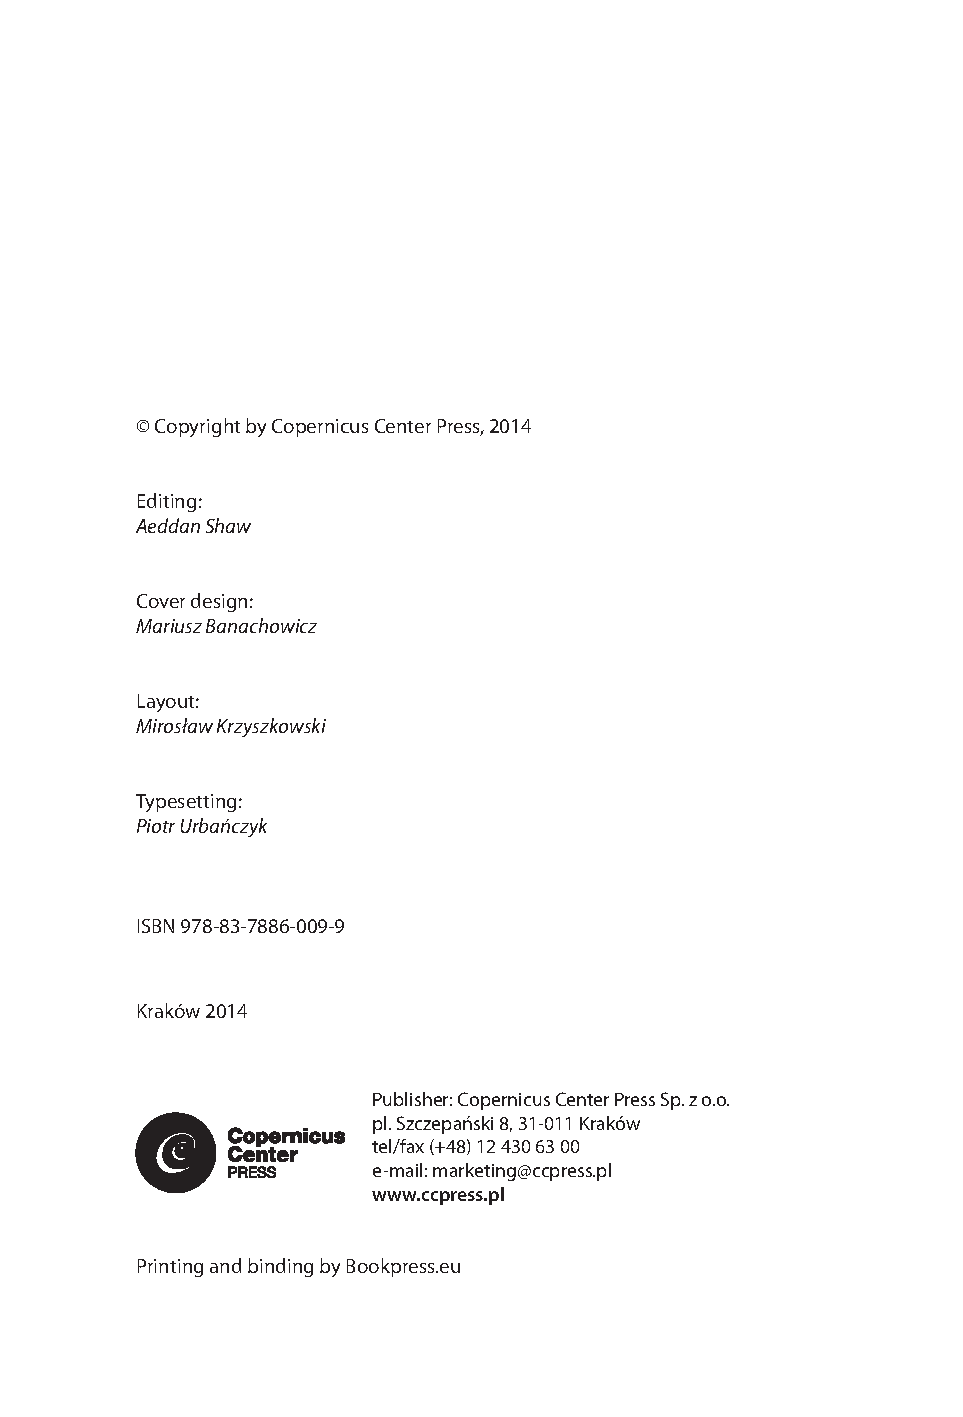
\includepdf[pages=1]{images/CT4.pdf}


%\thispagestyle{empty}
\vspace*{1.2in}%
\begin{flushright}
\rectitle{Zagadnienia Filozoficzne\\w Nauce}\par
\vspace*{.5in}%
\chaptitleeng{Philosophical Problems\\in Science}\par
\end{flushright}
\vfill
%\clearpage
%
%\thispagestyle{empty}

\vfill

\noindent\begin{czw}© Copernicus Center Press, \rok\end{czw}

\vfill

\begin{adres}
	\begin{pagname}\noindent\begin{czwad}Editorial Board\end{czwad}\\
		Editor-in-Chief: dr hab. Paweł Jan Polak\\
		Deputy Editor-in-Chief: dr hab. Janusz Mączka\\
		Honorary Editor: prof. dr hab. Michał Heller\\
		Editorial Secretary: Piotr Urbańczyk\\
		Section Editor (\textit{Emergence of the Classical}): dr Michał Eckstein
	\end{pagname}
\end{adres}


\vfill

\noindent\begin{czw}Cover design: Mariusz Banachowicz\end{czw}

\vskip.5em

\noindent\begin{czw}Adjustment and correction: Artur Figarski\end{czw}

\vskip.5em

\noindent\begin{czw}Technical editor: Artur Figarski\end{czw}

\vskip.5em

\noindent\begin{czw}Typographic design: Piotr Urbańczyk\end{czw}

\vskip.5em

\noindent\begin{czw}Typeset in \end{czw}\LaTeX

%\noindent\begin{czw}Skład: Artur Figarski\end{czw}


\vfill

\begin{adres}
	\begin{pagname}\noindent ISSN 0867-8286 (print format)\\
		e-ISSN 2451-0602 (electronic format)
	\end{pagname}
\end{adres}

\vfill

\begin{adres}
		\noindent\begin{czwad}Editorial Office\end{czwad}
	
		\noindent\begin{pagname}Zagadnienia Filozoficzne w Nauce
		
		\noindent Wydział Filozoficzny UPJPII
		
		\noindent ul. Kanonicza 9, 31-002 Kraków
		
		\noindent POLAND
		
		\vskip.3em
		
		\noindent e-mail: zagadnienia@upjp2.edu.pl
		
		\noindent www.zfn.edu.pl\end{pagname}
\end{adres}

\vfill

\begin{wrapfigure}{L}{.3\textwidth}
	\noindent\includegraphics[width=.29\textwidth]{images/ccp.pdf}
%\noindent\includegraphics[width=.27\textwidth]{images/ccp.pdf}
\end{wrapfigure}
\vskip.4em
%\noindent\parbox[t]{6cm}{
\begin{adres}
	\noindent\begin{pagname}Publisher: Copernicus Center Press Sp. z o.o.
		
		\noindent pl. Szczepański 8, 31-011 Kraków POLAND
		
		\noindent tel. (+48) 12 448 14 12
		
		\noindent e-mail: marketing@ccpress.pl
		
		\noindent www.ccpress.pl\\ \end{pagname}
	
	
\end{adres}
%}




%\clearpage

%	\thispagestyle{empty}
	\begin{flushright}%
	{\bigtitle{Zagadinienia\\Filozoficzne\\w Nauce\par}}%
	\vspace{0.2in}%
	{\chaptitleeng{Philosophical Problems in Science\par}}%
	\vspace{0.2in}%
	\hrule%
	{\LARGE\textbf{{\numerrzymski -- \rok}}}%
	\hrule%
	\end{flushright}%
%		\@mkboth{\czwit\contentsname}{\czwit\contentsname}%
	\vspace{0.5in}%
%
%\clearpage

%Spis tresci -------------------------------------------------

%{\thispagestyle{plain} \tableofcontents \clearpage}
%--------------------------------------------------------------------------------------------
%\newpage
%\thispagestyle{plain}
%\cleardoublepage
%\thispagestyle{plain}

%--------------------------------------


%\input{00a_malina.tex}

%\input{00b_introduction.tex}




%\ramkaart{Imię Nazwisko}
{Tytuł rozdziału.\\\chapsubtit{Podtytuł rozdziału}}
{Tytuł rozdziału. Podtytuł rozdziału}
{Tytuł rozdziału. Podtytuł rozdziału}

\lettrine[loversize=0.13,lines=2,lraise=0.00,nindent=0em,findent=0.2pt]%
{W}{}ielu filozofów i językoznawców twierdziło, że gdy identyfikujemy przedmioty, zarówno w języku, jak i w postrzeganiu, kierujemy się względami praktycznymi, potrzebami, wolą -- krótko mówiąc, swego rodzaju interesem, czy to gatunkowym (a więc ogólnoludzkim), czy to swoistym dla danej społeczności, cywilizacji czy jednostki. Wydaje się to kłócić z przeświadczeniem, że te przedmioty muszą istnieć, chyba że traktujemy to przeświadczenie jako jedną z wielu równouprawnionych wizji świata. Ta sama zasada wielości równosilnych perspektyw stosuje się a fortiori do języka metafizyki.

Tak więc powracamy tam, gdzie nasz horror bierze swój początek. Jakże mam trwać przy danym języku (czy jakimś szczególnym punkcie widzenia, z którego patrzę na świat, albo regule interpretacji całości doświadczenia), nie przyznając mu uprzywilejowanej poznawczej mocy? A jeśli pretenduję do dysponowania wyższym czy może nawet absolutnym językiem, to albo nadawałby się on tylko do mówienia o innych językach, nie zaś o rzeczywistości, do której się odnoszą, albo byłby standardowym językiem, a inne byłyby jego niekompletnymi dialektami. W tym drugim przypadku byłby to rzeczywiście boski język, absolutny i zawierający wszelkie wyobrażalne punkty widzenia. Lecz język taki jest niemożliwy; nawet Bóg, przemawiając ustami proroka, musiał się przełożyć na język ludzki; przekład jest niechybnie zniekształcony, a nam brak dostępu do oryginału. W przypadku pierwszym język mój (język pierwszego stopnia, język rzeczy) nie może wprawdzie rościć sobie pretensji do jakiejkolwiek pozycji uprzywilejowanej, lecz w tym języku nie sposób byłoby nieobecność owej pozycji wyrazić: by to uczynić, musiałbym swój język porzucić i przejść do super(czy meta-) języka -- ale w takim języku moje stanowisko, jako że szczególne, nie dałoby się wyrazić.

\myquote{
Gdy więc wielkodusznie powiadam: „wszystkie stanowiska metafizyczne są równie dobre”, sam żadnego stanowiska nie zajmuję, po prostu wyrażam zasadę tolerancji, która, jakkolwiek chwalebna, ma charakter formalny i nigdy nie wyda, czy choćby zainspiruje, żadnej metafizycznej idei. Lecz próbując zachować tę zasadę i obstawać zarazem przy swym szczególnym punkcie widzenia, popadam w niekonsekwencję, jako że twierdzę wtedy, iż „stanowisko moje jest tak samo dobre jak każde inne, mimo że jest nie do pogodzenia z żadnym innym”.

A jeśli tak mówię, nie mogę w zrozumiały sposób wyjaśnić, w jakim sensie to stanowisko jest moje, w przeciwieństwie do innych. Niestety, tolerancyjna wspaniałomyślność nie pozwala uciec od paradoksu samoodniesienia.
}

\noindent Leon Chwistek, logik i malarz, w wydanej w 1921 roku książce Wielość rzeczywistości sugerował istnienie czterech rodzajów wzajemnie niezależnych (a zatem przypuszczalnie nieinterferujących z sobą wzajem) rzeczywistości: rzeczy, takie jak je postrzega zdrowy rozsądek; rzeczy nauk fizycznych; wrażeń; i wyobraźni. Znajdują one swój artystyczny wyraz w malarstwie – odpowiednio: prymitywistycznym, naturalistycznym, impresjonistycznym, futurystycznym\footnote{To jest przypis dolny. Jeśli niezależne od siebie pokłady rzeczywistości wymagają dla swego opisu niezależnych języków, sugeruje to, że języki te są całkowicie nieprzekładalne; skoro tak, to w istocie można sądzić, że różne wizje świata współistnieć mogą w doskonałej wzajemnej obojętności}. Lecz wielość ta, dowodził, pozwala na dowolną liczbę równoprawnych poglądów na świat, z których żadnego nie można dowieść, lecz każdy jest do przyjęcia pod warunkiem, że nie próbuje zmonopolizować prawdy. Dopuszczalne stają się różne odpowiedzi na tradycyjne pytania, jak te o wolność woli, relację między ciałem a duchem, obiektywność wartości, jeśli zakres odniesienia ogranicza się do jednej lub niektórych spośród owych czterech rzeczywistości.

\noindent Leon Chwistek, logik i malarz, w wydanej w 1921 roku książce Wielość rzeczywistości sugerował istnienie czterech rodzajów wzajemnie niezależnych (a zatem przypuszczalnie
nieinterferujących z sobą wzajem) rzeczywistości: rzeczy, takie jak je postrzega zdrowy rozsądek

\section{Podtytuł 1 stopnia}

\noindent Teoria wielu -- jakkolwiek wyodrębnianych -- rzeczywistości, jeśli nawet w tym przypadku stworzona dla metafizycznej interpretacji malarstwa, proponuje przekonujący i kuszący obraz świata. Jednakże jako propozycja epistemologiczna nie jest w stanie -- czy to w wersji Chwistka, czy Williama Jamesa -- poradzić sobie z wciąż tą samą trudnością: jak dowieść wyższości pewnej teorii bytu w tym samym języku, w którym została wypowiedziana? Mieliżbyśmy utrzymywać, że twierdzenie „wszystko jest konieczne” jest równie prawomocne co twierdzenie „poza związkami logicznymi nic nie jest konieczne” i że doktryna, według której słowo „ja” nie ma odniesienia, jest nie mniej prawdziwa niż ta, wedle której cokolwiek ma odniesienie, jest względne w stosunku do „ja”?

\subsection{Podtytuł 2 stopnia}

\noindent Jeśli niezależne od siebie pokłady rzeczywistości wymagają dla swego opisu niezależnych języków, sugeruje to, że języki te są całkowicie nieprzekładalne; skoro tak, to w istocie można sądzić, że różne wizje świata współistnieć mogą w doskonałej wzajemnej obojętności: nie mogą być ze sobą konfrontowane ani między sobą sprzeczne. Ale twierdzenie, że nie mogą być konfrontowane, jest wyrażone w języku innym, wyższego stopnia, nie nadającym się do celów metafizycznych. I tu powraca ten sam kłopot: albo ograniczamy się do tego wyższego języka i wtedy werdykty nasze nie mają znaczenia dla rzeczywistych problemów, z których filozofia żyje, albo przyjmujemy pewną metafizyczną perspektywę i głosimy, że perspektywy tej, jako zamkniętej, nie da się zharmonizować z żadną inną ani też innej przeciwstawić -- i wtedy też, w wyniku tej samointerpretacji, perspektywa nasza jest bez znaczenia dla rzeczywistych problemów, z których filozofia żyje.

\sectionno{Podtytuł 1 stopnia}

\noindent Teoria wielu -- jakkolwiek wyodrębnianych -- rzeczywistości, jeśli nawet w tym przypadku stworzona dla metafizycznej interpretacji malarstwa, proponuje przekonujący i kuszący obraz świata. Jednakże jako propozycja epistemologiczna nie jest w stanie -- czy to w wersji Chwistka, czy Williama Jamesa -- poradzić sobie z wciąż tą samą trudnością: jak dowieść wyższości pewnej teorii bytu w tym samym języku, w którym została wypowiedziana? Mieliżbyśmy utrzymywać, że twierdzenie „wszystko jest konieczne” jest równie prawomocne co twierdzenie „poza związkami logicznymi nic nie jest konieczne” i że doktryna, według której słowo „ja” nie ma odniesienia, jest nie mniej prawdziwa niż ta, wedle której cokolwiek ma odniesienie, jest względne w stosunku do „ja”?

\subsection{Podtytuł 2 stopnia}

\noindent Jeśli niezależne od siebie pokłady rzeczywistości wymagają dla swego opisu niezależnych języków, sugeruje to, że języki te są całkowicie nieprzekładalne; skoro tak, to w istocie można sądzić, że różne wizje świata współistnieć mogą w doskonałej wzajemnej obojętności: nie mogą być ze sobą konfrontowane ani między sobą sprzeczne. Ale twierdzenie, że nie mogą być konfrontowane, jest wyrażone w języku innym, wyższego stopnia, nie nadającym się do celów metafizycznych. I tu powraca ten sam kłopot: albo ograniczamy się do tego wyższego języka i wtedy werdykty nasze nie mają znaczenia dla rzeczywistych problemów, z których filozofia żyje, albo przyjmujemy pewną metafizyczną perspektywę i głosimy, że perspektywy tej, jako zamkniętej, nie da się zharmonizować z żadną inną ani też innej przeciwstawić -- i wtedy też, w wyniku tej samointerpretacji, perspektywa nasza jest bez znaczenia dla rzeczywistych problemów, z których filozofia żyje.

\section{Podtytuł 1 stopnia}

\noindent Teoria wielu -- jakkolwiek wyodrębnianych -- rzeczywistości, jeśli nawet w tym przypadku stworzona dla metafizycznej interpretacji malarstwa, proponuje przekonujący i kuszący obraz świata. Jednakże jako propozycja epistemologiczna nie jest w stanie -- czy to w wersji Chwistka, czy Williama Jamesa -- poradzić sobie z wciąż tą samą trudnością: jak dowieść wyższości pewnej teorii bytu w tym samym języku, w którym została wypowiedziana? Mieliżbyśmy utrzymywać, że twierdzenie „wszystko jest konieczne” jest równie prawomocne co twierdzenie „poza związkami logicznymi nic nie jest konieczne” i że doktryna, według której słowo „ja” nie ma odniesienia, jest nie mniej prawdziwa niż ta, wedle której cokolwiek ma odniesienie, jest względne w stosunku do „ja”?

\subsection{Podtytuł 2 stopnia}

\noindent Jeśli niezależne od siebie pokłady rzeczywistości wymagają dla swego opisu niezależnych języków, sugeruje to, że języki te są całkowicie nieprzekładalne; skoro tak, to w istocie można sądzić, że różne wizje świata współistnieć mogą w doskonałej wzajemnej obojętności: nie mogą być ze sobą konfrontowane ani między sobą sprzeczne. Ale twierdzenie, że nie mogą być konfrontowane, jest wyrażone w języku innym, wyższego stopnia, nie nadającym się do celów metafizycznych. I tu powraca ten sam kłopot: albo ograniczamy się do tego wyższego języka i wtedy werdykty nasze nie mają znaczenia dla rzeczywistych problemów, z których filozofia żyje, albo przyjmujemy pewną metafizyczną perspektywę i głosimy, że perspektywy tej, jako zamkniętej, nie da się zharmonizować z żadną inną ani też innej przeciwstawić -- i wtedy też, w wyniku tej samointerpretacji, perspektywa nasza jest bez znaczenia dla rzeczywistych problemów, z których filozofia żyje.

\begin{thebibliography}{00}{Imię Nazwisko}
{Tytuł rozdziału. Podtytuł rozdziału}

\makeatletter
    \clubpenalty10000
    \@clubpenalty \clubpenalty
    \widowpenalty10000
\makeatother


\bibitem{Abc}
A.~Abc, \textit{Abc}...

\bibitem{Xyz}
A.~Abc, \textit{Abc}...

\end{thebibliography}



%\sekcja{Artykuły}{Articles}

%\begin{artengenv}{Claus Kiefer}
	{Does the quantum mechanical wave function exist?}
	{Does the quantum mechanical wave function exist?}
	{Does the quantum mechanical wave function exist?}
	{Institute for Theoretical Physics, University of Cologne}
	{I address the question whether the wave function in quantum theory
		exists as a real (ontic) quantity or not. 
		For this purpose, I discuss the essentials of the quantum formalism and emphasize the
		central role of the superposition principle. I then explain the measurement
		problem and discuss the process of decoherence. Finally, I address the
		special features that the quantization of gravity brings into the
		game. From all of this I conclude that the wave function really
		exists, that is, it is a real (ontic) feature of Nature.}
	{wave function, quantum mechanics, ontology, quantum formalism, superposition principle, measurement problem, decoherence, quantum gravity.}

% For Proceedings of Krakow Conference 2017
% revised version 10.5.2019






\section{Quantum theory}

\lettrine[loversize=0.13,lines=2,lraise=-0.05,nindent=0em,findent=0.2pt]%
{T}{}he title of my contribution may sound somewhat surprising, at least
at first glance. After all, the quantum mechanical wave function and
its generalizations in quantum field theory (generically here called 
$\Psi$) are standard tools in
quantum theory and its many applications in physics, chemistry, and
even biology. This is true, and one can definitely say that $\Psi$
exists in a mathematical sense. The question addressed here instead refers to
whether $\Psi$ can be attributed an ontic or merely an epistemic role,
that is, whether $\Psi$ can be attributed reality in the same way as,
for example, an electric field possesses, or whether it merely describes
something like an information catalogue (as Schr\"odinger once put
it). This is a question that has occupied physicists since the advent
of quantum theory in the 1920s and that still occupies them today;
see, for example, d'Espagnat \parencite*{despagnat_veiled_1995}, Kiefer \parencite*{kiefer_albert_2015},
or Boge \parencite*{boge_quantum_2018} and the many
references quoted therein. Here, I will argue that the answer to
the question posed in the title is definitely in the affirmative, and I
will try to put together the main arguments of why this is so and why
the wave function has an ontic (real) status. Some of these arguments
have been presented in an earlier article \parencite{kiefer_claus_emergence_2012}, to which I
will occasionally refer.  

At the heart of all of quantum theory is the {\em superposition
  principle}. It can be separated into a kinematical and a dynamical
version \parencite{joos_decoherence_2003}. The kinematical version expresses the fact that if
$\Psi_1$ and $\Psi_2$ are physical states, then 
$\alpha\Psi_1+\beta\Psi_2$ is again a physical state, where $\alpha$
and $\beta$ are complex numbers.  
For more than one degree of freedom, this leads to the important
concept of
{\em entanglement} ({\em Verschr\"ankung}) between systems \parencite{kiefer_albert_2015},
which plays a particular important role in modern developments
such as quantum information. The very concept of a quantum computer
relies on entanglement. 

It is clear that this kinematical version only makes sense if it is
consistent with the dynamics of the theory. But this is the case. The
fundamental equation is the Schr\"odinger equation (by which I include
its field theoretic generalization, the functional Schr\"odinger
equation), and this equation is {\em linear}: the sum of two
  solutions is again a solution. An importance consequence of the
  superposition principle is obvious: the space of what we may call 
``classical states'' form only a tiny subset in the space of all
possible states. A simple example is the superposition of two
localized states, each of which can describe a classical state, to a
nonlocal (and thus nonclassical) state. It must be emphasized that the
quantum mechanical wave functions are not defined on spacetime, but on
{\em configuration space} (cf. e.g. \cite{zeh_strange_2016} for a lucid conceptual
discussion). Except for the case of one particle, this is a
high-dimensional space: the dimension is $3N$ for a system of $N$
particles, and infinite in field theory.
Otherwise, there would be no entanglement between systems.

Entanglement is the central distinguishing feature of quantum theory.
As already Erwin Schr\"odinger put it \parencite[p.~555]{schrodinger_discussion_1935}:

\myquote{
I would not call that {\em one} but rather {\em the}
characteristic trait of quantum mechanics, the one that enforces
its entire departure from classical lines of thought. By the
interaction the two representatives (or $\psi$-functions)
have become entangled. \ldots Another way of expressing the
peculiar situation is: the best possible knowledge of a
{\em whole} does not necessarily include the best possible
knowledge of all its {\em parts}, even though they may be
entirely separated \ldots
}

The superposition principle has been experimentally tested
in uncountably many experiments \parencite{schlosshauer_decoherence:_2007,kiefer_albert_2015}.
Even before the term entanglement was coined, it was clear
that the electrons in a helium atom must be
entangled in order to lead to the correct observed binding energies 
\parencite{hylleraas_neue_1929}. Modern experiments include the interference of
biomolecules, the entanglement of photon pairs over distances of
hundreds of kilometres, and the observation of neutrino oscillations,
to name only a few; see, for example, Deng et al. \parencite*{deng_quantum_2019}
for an experiment involving interference between light sources
separated by 150~million kilometres. There can thus be no doubt that
the superposition 
principle holds. The generation of ``macroscopic'' superpositions is
being seriously considered; see, for example, Clarke and Vanner \parencite*{clarke_growing_2018}. 
 
In the mathematical language of quantum theory,
the validity of the superposition principle is encapsuled in the use
of vector spaces for the quantum states (wave functions). The stronger
concept of a Hilbert space (using a scalar product between states) is
motivated by the probability interpretation of quantum theory, which
by itself is connected to the ``measurement problem'' discussed since
the early days of the theory. This measurement problem refers, in
fact, to the only class of situations in which the superposition
principle seems to break down.

What is the measurement problem? Let us consider the simple situation
of an apparatus, A, coupled to a system, S:\footnote{This and the
  following diagramme are taken from our monograph \parencite{joos_decoherence_2003}.}
\begin{figure}[h]
\begin{center}
\setlength{\unitlength}{1cm}
\begin{picture}(5,1) \thicklines %\linethickness{1mm}
\put(0,0){\framebox(2,1){S}}
\put(3,0){\framebox(2,1){A}}
\put(2,0.5){\vector(1,0){1}}
\end{picture}
\end{center}
\end{figure}
I emphasize that both system and apparatus are described by quantum
theory. This analysis goes back to John von Neumann \parencite{von_neumann_mathematische_1932}.
The simplest situation of an interaction is the ``ideal
measurement'': the system is not disturbed by the apparatus, but the
state of the apparatus becomes correlated with the state of the
system. If S is in a state $|n\rangle$ and A in an initially
uncorrelated state $|\Phi_0\rangle$, the total state of S and A evolves as
\be
|n\rangle|\Phi_0\rangle \stackrel{t}{\longrightarrow}
|n\rangle|\Phi_n(t)\rangle.
\ee
The measurement problem appears when we consider a superposition of
possible states $|n\rangle$.\footnote{In the simple situation of
  spin-1/2, one would have two states  $|n\rangle$, one corresponding
  to (say) spin up and the other to spin down.}
This leads to the evolution:
\be
\lb{super}
\left(\sum_n c_n|n\rangle\right)|\Phi_0\rangle
    \stackrel{t}\longrightarrow\sum_n c_n|n\rangle
    |\Phi_n(t)\rangle,
\ee
where $|\Phi_n(t)\rangle$ is the resulting state (`pointer state') of
A. 
But \eqref{super} is a {\em macroscopic} superposition! 
Since such superpositions\footnote{An especially impressive example is
  Schr\"odinger's cat.} are not observed, John von Neumann postulated
the occurrence of a ``collapse of the wave function'' in
measurement-like interactions; he did not, however, present a
dynamical equation for such a collapse, which must be unitarity violating
and is thus in conflict with the Schr\"odinger equation.

In more recent years, various models of wave function collapse have
been presented in the literature and possible experimental tests have
been discussed.\footnote{See, for example, Bassi et al. \parencite*{bassi_models_2013} for a
  comprehensive review.} It must be emphasized that most of these models only
make sense if the wave function acquires a real (ontic) status. This
is different from its role in the Copenhagen interpretation of quantum
theory, where the `collapse' has the mere formal meaning of an
information increase. We shall see in the next section how we can
proceed without assuming a dynamical collapse, that is, without
violating the unitarity of quantum theory. 

Before doing so, I want to conclude this section with some remarks on
relativistic quantum theory, in particular the Dirac equation. 
The Dirac spinor appearing there should not be
confused with the wave function discussed above. The spinor is {\em
  not} defined in configuration space; it is defined on a classical
(in general four-dimensional) spacetime. It thus cannot describe
entanglement and can only serve to address one-particle situations;
it can describe correctly the situation in the hydrogen atom, but
cannot even be formulated for the helium atom.\footnote{Cf. in this
  context Zeh \parencite*{zeh_strange_2016}.} Relativistic quantum theory is only consistent
in the form of quantum {\em field} theory; the Dirac equation follows
from quantum electrodynamics (QED) for the special case of
one-particle excitations.      
When we talk here about the ontological status of $\Psi$, this refers in
the general case of quantum field theory to wave {\em functionals}.
These functionals are defined on the configuration space of all
fields; in the case of QED, for example, this is the space of all
vector potentials and charged Grassmann (anti-commuting) fields.


\section{Decoherence}

How can one understand the nonobservation of superpositions such as
\eqref{super} without advocating an explicit collapse?
The key role in answering this question is played by the presence of
the ubiquitous environment for the apparatus. This was clearly
recognized in the pioneering work by H.-Dieter Zeh in
1970.\footnote{The original reference is Zeh \parencite*{zeh_interpretation_1970}. See Joos \textit{et
  al}. \parencite*{joos_decoherence_2003} for details and references.} 
`Environment' is here a technical terms that stands for additional
degrees of freedom whose interaction with the `apparatus' (or other
systems under consideration) cannot be avoided. In concrete examples, 
these may be air molecules or photons that scatter off the
`apparatus'. One thus has instead of the above diagramme the 
following situation:
\enlargethispage{-.75\baselineskip}

\begin{figure}[h]
\begin{center}
\setlength{\unitlength}{1cm}
\begin{picture}(5,1)(-0.25,-0.25) \thicklines %\linethickness{1mm}
\put(0,0){\framebox(1,0.5){S}}
\put(1.5,0){\framebox(1,0.5){A}}
\put(1,0.25){\vector(1,0){0.5}}
\put(3,-0.25){\framebox(1.5,1){E}}
\put(2.5,0.15){\vector(1,0){0.5}}
\put(2.5,0.25){\vector(1,0){0.5}}
\put(2.5,0.35){\vector(1,0){0.5}}
\put(-0.25,-0.25){\dashbox{0.1}(3,1){}}
\end{picture}
\end{center}
\end{figure}

Here, E stands for the environmental degrees of freedom, and the three
arrows between A and E indicate the many degrees of freedom.

If the environment is in an initial state $|E_0 \rangle$,
 the superposition principle for the whole system of S, A, and E leads to
\be
\lb{super2}
\left( \sum_n c_n|n\rangle|\Phi_n\rangle\right)|E_0 \rangle
  \quad  \stackrel{t}\longrightarrow \quad
   \sum_n c_n|n\rangle |\Phi_n\rangle |E_n\rangle. 
\ee
But this is an even more macroscopic superposition than \eqref{super}
because it not only includes system and apparatus, but also the many
degrees of freedom of the environment. Has the situation not become
worse now? The answer is no. The reason is because the degrees of
freedom of the environment are in general not accessible; when
dealing with S and A only, one has to trace them out and to consider
instead the reduced density matrix of S and A alone, from which all
{\em local} observations follow. Since different environmental states
are in general orthogonal (because they can discriminate between
different states of A), $\langle E_n|E_m \rangle \approx \delta_{nm}$,
the reduced density matrix assumes the form 
\be
\lb{rho}
\rho_{\rm SA} \approx \sum_n |c_n|^2 |n\rangle\langle n|
   \otimes |\Phi_n \rangle \langle \Phi_n |,
 \ee
which is approximately (but not identically) equal to a classical
stochastic mixture. The information about the original superposition
of \eqref{super} has now been transferred to a nonlocal correlation
between S and A on the one side, and E on the other side. They are no
longer observable at S and A itself:
``The interferences exist, but they are not {\em there}.''
The various system states $|n\rangle$ are distributed with
probabilities $|c_n|^2$ according to the Born rule of quantum theory. 
(It should be noted, though, that the very notion of density matrix is
based on the validity of the Born rule.) 

This irreversible emergence of classical properties (nonobservability
of interference terms) through the unavoidable interaction with the
environment is called {\em decoherence}. It has been explored in the
last decades, both experimentally and theoretically.\footnote{Major
  reviews are Joos et al. \parencite*{joos_decoherence_2003},
  Zurek \parencite*{zurek_decoherence_2003}, Schlosshauer
  \parencite*{schlosshauer_decoherence:_2007}.
  Crucial experiments are also discussed in Haroche \parencite*{haroche_controlling_2014}.}  
According to decoherence, macroscopic objects {\em appear}
classically, although they are fundamentally described by quantum
theory. Decoherence is a process that can be treated entirely within
standard quantum mechanics and which can be based on realistic
processes discusses in a quantitative manner.\footnote{Such
  quantitative calculations were presented for the first time in Joos
  and Zeh \parencite*{joos_emergence_1985}.} 

What are the consequences of this for the interpretation of quantum
theory in general and for the wave function in particular?
If the superposition principle and the Schr\"odinger equation are
universally valid, one arrives at what is called the Everett or
many-worlds interpretation (see e.g. \cite{despagnat_veiled_1995,zeh_strange_2016}).
Unitary
quantum theory is then exact and never violated. The dead and the
alive Schr\"odinger cat, for example, then indeed exist simultaneously
in different ``Everett branches'', and also the observer seeing the
cat exists in two versions. In this point of view, the wave function
definitely has an ontic status and exists in the way discussed above.
The Everett interpretation together with decoherence makes the
measurement problem obsolete.

A question often asked is about the derivation of the probability
interpretation (the Born rule) in the Everett picture. This has been
discussed at length in the literature; see, for example, Zurek
\parencite*{zurek_wojciech_hubert_quantum_2018}
and the references therein. The probability interpretation only makes
sense for situations in which decoherence is effective, because only
then the various alternatives can be treated independently and can be
assigned probabilities. Whether the Born rule can then really be {\em
  derived} or only be made plausible, is a contentious issue. But what is
clear that the Everett interpretation together with decoherence and
the Born rule gives a consistent picture that is not in need
of completion. 

The Everett interpretation is the simplest one at the level of the
mathematical formalism. The fundamental equations are all linear. It
is not a simple interpretation if one sticks to a classical picture of
the world. This is what the main alternative -- explicit collapse
models -- wants to achieve \parencite[see e.g.][]{bassi_models_2013}. But this
requires a modification of the usual formalism by bringing in
nonlinearities or stochastic terms. Also here, the wave function
assumes an ontic status. The main task is to work out concrete models
and to explore their experimental status. 

A rather mild modification is the de~Broglie--Bohm
theory. The Schr\"odinger for $\Psi$ is left untouched, but
in addition particle (or classical field) configurations are
introduced. The wave function, which is defined in configuration space,
acts as a kind of `guiding field' for the particles in ordinary
space. There, too, it has an ontic status and can thus be assumed to
exist. At least in nonrelativistic quantum mechanics, the predictions
of the  de~Broglie--Bohm theory agree with the predictions of standard quantum
theory.

The prototype of an epistemic point of view is the Copenhagen
interpretation. There, $\Psi$ merely provides an increase of information
during a measurement and has no physical existence on its own -- only
the classical concepts such as particle posititions have. But is such
a point of view really consistent and satisfactory?  This is hard to
believe. New light on these interpretational questions is shed by
entering the realm of quantum gravity and quantum cosmology. This is
the topic of my final section.

 

\section{Quantum gravity}


In 1957, a group of distinguished physicists met at the University of
North Carolina to explore the prospects of gravitational physics.
This also included the possible quantization of the
gravitational field. In the discussion, Richard Feynman came up with
the following 
gedanken experiment. In a Stern--Gerlach type of setting, a particle
is brought into a superposition of, say, spin up and spin
down. Introducing some interconnections to a macroscopic object, say
a ball of 1~cm diameter, one can bring the ball into a superposition of being
translated upwards and downwards. But this corresponds to a
superposition of two measurable gravitational fields (measurable e.g. with a
Cavendish balance). Feynman then states \parencite{de_witt_proceedings:_1957}:

\myquote{
\ldots if you believe in quantum mechanics up to any level then you
have to believe in gravitational quantization in order to describe
this experiment. \ldots It may turn out, since we've never done an
experiment at this level, that it's not possible \ldots that there is
something the matter with our quantum mechanics when we have too much
{\em action} in the system, or too much mass---or something. But that
is the only way I can see which would keep you from the necessity of
quantizing the gravitational field. It's a way that I don't want to
propose. \ldots 
}

\begin{figure}[h]
	\centering
   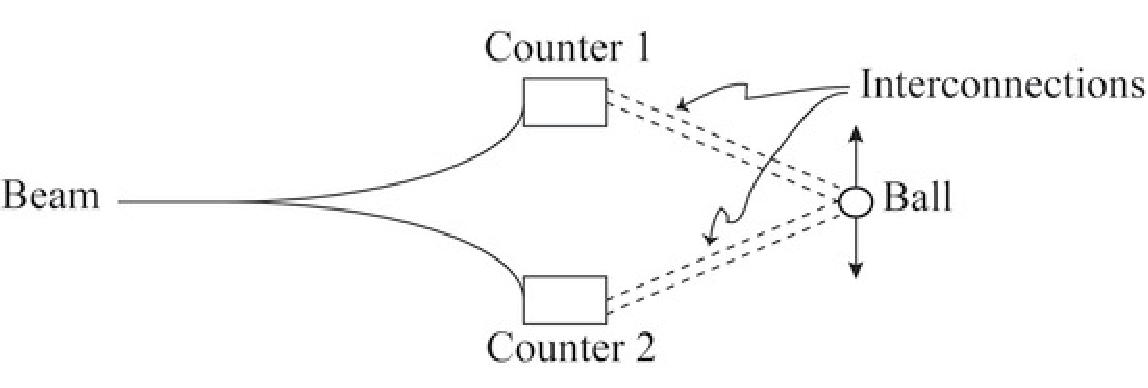
\includegraphics[width=0.8\textwidth]{ART_Kiefer/Kiefer_img.pdf} 
\caption{Feynman's gedanken experiment in which a microscopic
  superposition is transferred to a macroscopic one of a ball being
  simultaneously at two different places. Figure adapted from \cite{de_witt_proceedings:_1957}.}
\end{figure}

In order words, unless one assumes that the superposition principle
and the standard formalism of quantum theory is violated when
gravitational fields play a role (as, for example, Lajos Di\'osi and
Roger Penrose 
envisage), the quantization of gravity seems unavoidable. The majority
of researchers thus accepts the assumption of 
extrapolating the standard linear formalism of quantum theory to
quantum gravity. This holds for almost all of the existing approaches,
from canonical and covariant quantum gravity up to string theory
\parencite{kiefer_quantum_2012}.

At present, there is a discussion about the possibility to observe
gravitational superpositions in the laboratory. There are proposals
to probe a nonclassical gravitational field generated by
two masses each of which is superposed at two locations
\parencite[see e.g.][]{marletto_witness_2017}
or to probe such a field generated by the superposition
of one mass in the spirit of Feynman's proposal cited above
\parencite[see e.g. the remarks in][]{schmole_micromechanical_2016}.
The
observability of such superpositions also meets with criticism 
\parencite{anastopoulos_comment_2018}.

What are the consequences of quantum gravity for our question about the
reality of the wave function? In order to answer this question, it is
sufficient to use the simplest and most conservative approaches to
quantum gravity, which is quantum geometrodynamics.\footnote{Details
  and relevant references can be found, for example, in my monograph
  \parencite{kiefer_quantum_2012}.} One arrives at this theory when asking the
following question: what is the quantum formalism that gives back
Einstein's equations in the semiclassical (WKB) limit? This is analogous
to the heuristic procedure that Erwin Schr\"odinger led to his
equation in 1926.

The canonical formalism of general relativity discloses the real
dynamical quantity of the theory: it is the {\em three-dimensional}
geometry. The configuration space is thus the infinite-dimensional
space of all three-dimensional metrics, with an additional constraint
which guarantees that metrics related by coordinate transformations are
counted only once. The theory possesses four local constraints, which
after Dirac quantization are heuristically transformed into quantum
constraints on physically allowed wave functionals. 
In a shorthand notation, they read
\be
\label {wdw}
\hat{H}\Psi=0,
\ee
where $\hat{H}$ denotes the Hamilton operator of all gravitational and
nongravitational degrees of freedom. The functional $\Psi$ is defined
on the space of three-metrics and nongravitational fields. Equation
\eqref{wdw} is also called Wheeler--DeWitt equation.\footnote{More
  precisely, if written out, \eqref{wdw} includes the Wheeler--DeWitt
  equation and the diffeomorphism constraints.} 

One recognizes from \eqref{wdw} the absence of any external time parameter 
\parencite[see in this context][]{kiefer_does_2015}.
This is obvious for conceptual
reasons. In classical relativity, spacetime (four-geometry) plays the
same role that a particle trajectory plays in mechanics. After
quantization, spacetime has disappeared in the same way as the
particle trajectory has disappeared in quantum mechanics. But whereas
in quantum mechanics Newton's absolute time $t$ has survived, 
no such absolute time is present in Einstein's theory.  
As a result, the fundamental quantum gravity equations are timeless.

Of special concern here is quantum cosmology -- the application of
quantum theory to the Universe as a whole. In the simple case of a
Friedmann universe with scale factor $a$ and a conformally coupled
scalar field $\chi$, the Wheeler--DeWitt equation assumes the form
(after some rescaling and with a suitable choice of units):
\be
\lb{qc}
\hat{H}_0\psi(a,\chi)\equiv (-H_a+H_{\chi})\psi\equiv
\left(\frac{\partial^2}{\partial a^2}-\frac{\partial^2}{\partial\chi^2}
-a^2+\chi^2\right)\psi=0.
\ee

How can one interpret such equations? At the most fundamental level, 
there is no time and there are no classical observers who could
perform measurements. Therefore, the Copenhagen interpretation which
requires the need of classical measurement agencies from the outset,
is inapplicable.  
The question thus arises in which limit
approximate notions of time and observers (more generally, of classical
properties) emerge and what relevance this emergence has for the
interpretation of the wave function. 

Such a limit exists and is well understood \parencite{kiefer_quantum_2012,kiefer_does_2015}. It
is similar to the Born--Oppenheimer approximation in molecular
physics. If one adds inhomogeneous degrees of freedom to the
Hamiltonian in \eqref{qc}, the Wheeler--DeWitt equation is of the form
\be 
\left(H_0+\sum_nH_n(a,\phi,x_n)\right)\Psi(\alpha,
 \phi,\{ x_n\})=0,
\ee
where the $x_n$ stand for the inhomogeneities (gravitational waves,
density perturbations). 
Writing $\Psi=\psi_0\prod_n\psi_n$ and assuming that
$\psi_0$ is of WKB form, that is, $\psi_0\approx C\exp(\I S_0/\hbar)$
(with a slowly varying prefactor $C$), one gets
\be
\I\hbar\frac{\partial\psi_n}{\partial t} \approx H_n\psi_n
\ee
with
\bdm
\frac{\partial}{\partial t}:= \nabla S_0\cdot\nabla.
\edm
This is nothing but a set of time-dependent Schr\"odinger equations
for the inhomogeneities with respect to a time variable $t$ that is
defined from the homogeneous cosmological background;
$t$ is also called `WKB time' and controls the dynamics in this
approximation. Only in this limit can one talk about the probability
interpretation of quantum theory and the existence of observers. It is
thus not at all obvious whether the standard notion of Hilbert space
need, or even can, be extrapolated to the level of full quantum
gravity (beyond this level of the Born--Oppenheimer approximation).

In quantum cosmology, 
 arbitrary superpositions of the gravitational
field and matter states can occur. How can we understand the emergence
of an (approximate) classical Universe? This is achieved by the
process of decoherence introduced above \parencite{kiefer_claus_emergence_2012}. 
Decoherence is a process in
configuration space, and the irrelevant degrees of freedom can be
taken to be part of the inhomogeneities $x_n$. In this way, the scale
factor $a$ and the field $\chi$ can be shown to assume classical
properties. The same then holds for WKB time $t$, which is constructed
from these background variables. 
After this classicality is understood, one can investigate
decoherence for some relevant inhomogeneous degrees of freedom; these
include the inhomogeneities of an inflaton scalar field and
of the metric, giving rise, after decoherence, to the observed CMB
anisotropies and the (not yet discovered) primordial gravitational
waves. In all these considerations, the wave function is assumed to be
real (ontic); this is also the case if one applies collapse models to
quantum cosmology. I should also mention that even the problem of the
arrow of time can, at least in principle, be understood in the
framework of timeless quantum cosmology \parencite{zeh_physical_2007}.

It is clear that the debate about the correct interpretation of
quantum theory will continue, at least until a clear experimental
decision is reached (which could take quite a while). In this
contribution, I have collected arguments which strongly support the
point of view that the wave function is real (ontic), in the same way
as, say, an electric field, is real. Thus, the wave function {\em
  exists}. The perhaps most important open question is: what is the
configuration state for the wave functional at the most fundamental
level? In canonical quantum gravity, it is the space of
three-geometries plus nongravitational fields; what it is at the level
of a fundamental quantum theory of all interactions, is unknown.



%%%%%%%%%%%%%%%%%%%%%%%%%%%%%%%%%%%%%%%%%%%%%%%%%%%%%%%%%%%%%%%%%%

\paragraph{Acknowledgements}

I am grateful to the organizers of the conference
{\em On What Exists in Physics} (Krak\'ow, October~2017) for inviting
me to such an  
inspiring event. I am, in particular, indebted to Professor Micha\l\
Heller for many interesting discussions.

\nocite{einstein_can_1935}
%%%%%%%%%%%%%%%%%%%%%%%%%%%%%%%%%%%%%%%%%%%%%%%




\end{artengenv}

%\begin{artengenv}
	{Tadeusz Sierotowicz}
	{Where are Sunspots? The Practical Method of Galileo as an example of Mental Model}
	{Where are Sunspots? The Practical Method of Galileo\ldots}
	{Where are Sunspots? The Practical Method of Galileo as an example of Mental Model}
	{Copernicus Center for Interdisciplinary Studies,\\
		Istituto di Scienze Religiose di Bolzano e IISS Gandhi di Merano}
	{After the publication of \textit{Sidereus Nuncius} Galileo, in the controversy with Ch.
		Scheiner, developed several arguments on behalf of the hypothesis that sunspots are contiguous to the surface of the
		Sun, and presented them in his \textit{Istoria e dimostrazioni intorno alle macchie solari e loro accidenti}
		(Rome 1613).
		%brakuje bibliografii
		One of them, named by Galileo a Practical Method, advocates very clearly the correctness of the
		hypothesis. In the paper the method in question is briefly described. It is argued that the Practical Method is not a
		thought experiment, but rather a mental model proposed precisely in order to solve the problem of sunspots’ location. }
	{sunspots, Galileo’s practical method, mental models, early modern science.}




\section{Introduction}

\lettrine[loversize=0.13,lines=2,lraise=-0.03,nindent=0em,findent=0.2pt]%
{A}{}fter Galileo discovered many celestial novelties through his telescope, as described in the widely read
\textit{Sidereus Nuncius}, his \textit{vis polemica} found a space in the sunspot dispute with the Jesuit priest
Christopher Scheiner (\cite[pp.238–259]{camerota_galileo_2004}; \cite[chap.2.6]{fantoli_galileo:_2003};
\cite{heilbron_galileo_2010,galilei_sunspots_2010-1,shea_galileo_1970,sierotowicz_o_2013})\footnote{Bibliographical note: the
\textit{opera} of Galileo Galilei discussed in the paper can be easily found on the Web: \textit{Istoria e
dimostrazioni\ldots}, \parencite{galilei_istoria_1613} see, e.g., copy of the National Library of Florence: BNCF -
II 461, the Nencini collection: brunelleschi.imss.fi.it/bibliotecagalileo; [\textcolor{black}{Accessed 23 Dec. 2010]}.
In the national edition of the works of Galilei, \textit{Istoria e dimostrazioni\ldots} can be found in the fifth volume:
\parencite[pp.25–239]{favaro_opere_1895}.
Favaro’s edition is cited here with the abbreviation OG, followed
by the number of the volume, the page number, and the verse number. For the English translation, see
\parencite{galilei_sunspots_2010}. Figures: For all details, see
\parencite{sierotowicz_o_2013}.
}. In this article, I pay special attention to a few pages from \textit{Istoria e dimostrazioni intorno alle macchie
solari e loro accidenti}
\parencite{galilei_istoria_1613},
which has been largely neglected by scholars. In the
work, the Pisano\footnote{Galileo is often referred to as the Pisano, after the city of his birth.} presented what he
himself called the most powerful reason in favour of his thesis about the location of sunspots. This is an original
method, called the Practical Method
\parencite[see OG V, 121.5;][p.112]{galilei_sunspots_2010},
through which
Galileo tried to prove his hypothesis by combining in a paradigmatic way sensible experiences (observations) and
necessary demonstrations (a geometrical model).

Galileo Galilei, in opposition to Christopher Scheiner, considered sunspots a phenomenon that exist on the surface of
the Sun and, as a consequence, participate in the rotation of the solar globe. However, according to Scheiner, sunspots
are just shadows of the passage of planets distant from the Sun through the solar disk. All these planets have to move
with an angular velocity that is equal to the angular velocity of the rotation of the Sun.

To decide which of these two theories is right, Galileo proposed several arguments. One of them, a sort of cinematic and
geometric reasoning, was based on the variation of the relative distance between the two spots moving along the same
parallel from the edge of the solar disk towards its centre. The Pisano noted that the observed distance between such
two sunspots changes in a particular way because of the projection on the observation plane of the segment between the
spots according to the angle that the segment forms with the plane of observation. Galileo developed a geometrical
model of this situation in his work on sunspots mentioned above (Fig. \ref{sier-fig1}). 

The apparent distance between two sunspots is normally smaller than the actual distance between them. However, on one
occasion, namely, when the segment between two spots is parallel to the observation plane, the length of the segment
and the length of its orthogonal projection onto the observation plane will be the same. This happens when the straight
line joining the observer’s eye with the centre of the Sun is aligned with the centre of the segment that joins the
spots (Fig. \ref{sier-fig5}). Of course, this situation is rather exceptional, but Galileo was lucky enough to observe it for two
sunspots on 01 July 1613 and 05 July 1613, respectively (Fig. \ref{sier-fig2} and \ref{sier-fig3}). Extraordinary, masterly executed drawings
representing these observations were printed in \textit{Istoria e dimostrazioni\ldots. }In fact, on July 5, 1613, spots A
and B appeared to be symmetrically located with respect to the centre of the solar disk. This particular observation
allowed Galileo to develop and apply the Practical Method. 

\section{The Practical Method}

First, Galileo noted that ``because the distance between the Sun and us is very great in proportion to the diameter of
its body''
\parencite[see OG V, 121.5;][p.112]{galilei_sunspots_2010}
some preliminary premises, also of a physical
nature, for his model can be made: 

\begin{enumerate}
	\item The rays that reach the eye of the terrestrial observer can be considered as parallel lines (see the rays ZDG, OLI,
	and QP in Fig. \ref{sier-fig1});
	\item Sunspots are located on the same latitude and pass through the centre of the solar disk or very close to it; and
	\item This situation occurs in the case of two spots, A and B (see Fig. \ref{sier-fig2} and \ref{sier-fig3}).
\end{enumerate}

Starting with these suppositions, Galileo constructed the geometric model of sunspot observations. The plane of the
drawing (Fig. \ref{sier-fig1}) corresponds to the plane passing through the observer, the centre of the Sun, and the parallel
(practically the equator) on which the sunspots A and B are located. The GDZ line, coming out from the centre of the
Sun G, goes towards the terrestrial observer to whom the spots appear projected on the plane perpendicular to the plane
just mentioned and passing through the centre of the Sun (the observation plane). Let CDE be the semicircle
representing the surface of the Sun, or the parallel on which the A and B spots move, and let the points on the CGE
segment correspond to the observed positions of sunspots in an orthogonal projection on the observation plane. The
points L and H are the sunspots A and B, respectively, observed on 01 July 1613 (Fig. \ref{sier-fig2}). The actual distance between
these spots is equal to the HL chord, but because of the projection effects, these spots are observed as points F and
I, and their observed distance is equal to the length of the FI segment. It is easy to see that in a situation where
the HL segment is symmetrical with respect to the GDZ line, the observed distance should be equal to the length of the
HL segment because the HL, FI, and CGE segments are parallel. This situation actually occurred on 5 July 1613 (see Fig.
\ref{sier-fig3} and \ref{sier-fig5}).

Naturally, the construction described above corresponds to the hypothesis that sunspots are supposed to be located on
the surface of the Sun, or very near to it. What if the spots are but the shadows of a distant planet (Scheiner’s
hypothesis)? Let us now imagine that the phenomenon of the spots is caused by a transition through the solar disk of
objects distant from the surface of the Sun that are about 1/20th of the diameter of the solar disk. The objects in
question therefore move on the MNO semicircle (Fig. \ref{sier-fig1}). In this case, sunspots should be collocated in points N and O,
and their real distance should correspond to the segment NO. It is easy to find out using a compass that the segment NO
is shorter than the HL one. Nevertheless, even in this case, the observed distance corresponds to the FI segment
because the geometric construction represents the way in which the mind and the eye of the terrestrial observer builds
images of the spots. How to decide which of the two situations, clearly different, reflects the real situation? To put
it briefly: where are sunspots -- on the MNO or on the CDE semicircle?

To answer this question, Galileo used a simple and ingenious method, inspired by the observation record of 05 July 1613.
Let the observer execute the drawing that represents this observation and its geometrical reconstruction on the same
scale; that is, let the observer trace the circle that represents the solar disk with the same opening of the compass
for both the geometric reconstruction (Fig. \ref{sier-fig1}) and the recording of the observations (Fig. \ref{sier-fig2} and \ref{sier-fig3}). In these
circumstances, the distance between spots A and B on 05 July directly gives the length of the chord that corresponds to
the real distance between the sunspots in the scale adopted for the drawing. 

Therefore, should the spots be on the surface of the Sun, it would correspond to the HL segment; otherwise, it would
correspond to the NO segment. A graphical manipulation shown on Fig \ref{sier-fig1} and \ref{sier-fig4} clearly indicates that the AB distance
observed on July 1 corresponds to the length of the FI segment. At the same time, reiterating the same operation for
Fig \ref{sier-fig1} and \ref{sier-fig3}, and thus arriving at Fig. \ref{sier-fig5}, it becomes clear that the distance between spots A and B on 5 July 1613 are
equal to the length of the HL segment, which is significantly greater than the length of the NO segment. This confirms
Galileo’s hypothesis.

Galileo must have had this procedure in mind. In fact, in the \textit{Istoria e dimostrazioni\ldots} he wrote, ``now if one
looks at the illustration of the fifth day [Fig. \ref{sier-fig3}], [\ldots] one will find that [the] distance [of the spots] A and B would
be exactly equal to the chord HL. This can in no way happen if their revolution takes place along a circle at any
distance whatsoever from the surface of the Sun''
\parencite[see OG V, 122.34-36;][p.115]{galilei_sunspots_2010}.
Then, he proposed the reasoning summarised above, calculating subsequently the numerical values of the difference
between chords in question (see OG V, 123).
%tu nie ma bibliografii

\section{The Practical Method and its Application}

The Practical Method is a brilliant argument that makes it possible to distinguish between two hypotheses on the
location of sunspots based on observations using a simple and immediate measurement based on a properly scaled
geometric model. The procedure seems to have innovative features. On the one hand, Galileo built a geometric model of
the phenomenon, but on the other hand, the model itself acts as a sort of measuring instrument that allows one to
resolve the dispute between two hypotheses with reference to the observations. It can therefore be said that the
graphical reasoning based on the geometrical model of the event (Fig. \ref{sier-fig5}) permits one to assign a numerical value to a
physical quantity (a distance between sunspots) and solve the problem.

A \textit{sine qua non} condition for such a reasoning to work is to assign the same value to the diameter of the solar
disk both in the construction of the geometric model and for the drawings representing the observations. Galilei
followed precisely this method. In fact, I have analysed a copy of Galileo’s treatise on sunspots from the Early
Printed Books Collection of the Jagiellonian Library in Cracow (593892 II). Here are the results of my measurements
performed on the drawing that corresponds to Fig. \ref{sier-fig1} (accuracy of ± 1 mm.):
\medskip

{\centering
HL = 60mm / ON= 52mm / GM = 69mm / FI = 42mm /\\CE = 123mm / CG = 62mm
\par}
\smallskip

In the same volume, the distance between the sunspots AB is, respectively, 42 mm (observation on 1 July: the diameter of
the solar disk is 123 mm) and 61 mm (observation on 5 July: the diameter of the solar disk is 122 mm).

Therefore, my measurements within the margin of errors seem to indicate that the length of the HL segment is equal to
the distance between the AB spots on 5 July, which in principle solves the ongoing dispute between Galileo and
Scheiner. Of course, things are not that simple because, first, the spots are not exactly point like, and second, they
change shape continuously, moving with their own motion.

In the \textit{Istoria e dimostrazioni\ldots} Galileo applied the Practical Method to other situations, using it as a
starting point for the prediction of the probable results of some possible sunspots observations
\parencite[see OG V, 124.13-21;][p.116]{galilei_sunspots_2010}.
 Suppose, for example, that spot A is collocated
at the edge of the solar disk in point C (Fig. \ref{sier-fig1}), and spot B in point H; then, the arc CGH would be equal to 4°.
Assuming that the GC radius is of 10000 units and the GM radius is of 10100, then the lengths of both the CH, and the
RN segments can be easily calculated; the CH segment would be of 419 units, and the RN of 94 units. The effect would
then be extremely strong (CH/RN = 4.46 versus HL/ON = 1.12 in Fig. \ref{sier-fig5}). Unfortunately, Galileo did not find any
observations corresponding to the situation in question.

\section{The Practical Method -- Methodological Aspects}

How to interpret Galileo’s reasoning? The Practical Method has some characteristics of what is defined in the literature
as an epistemic image. Such visual structures usually serve as a starting point for the formulation and development of
a given theory. The Feynman diagrams are often indicated as an example of this.

Galileo began with some hypotheses that simplified the description of the observational situation (e.g. the parallel
rays that reach the observer) and then constructed a geometric model that, through some mathematical calculations,
permits one to depict the evolution of the phenomenon. The model permits the prediction of the results of the
observations. Galileo’s two-dimensional model becomes, in a sense, a sort of measuring instrument that allows one to
compare directly the two hypotheses by referring them to the observations, solving in this manner a theoretical
problem. 

Thus, it seems reasonable to state that the Practical Method is a reasoning on which is based the argument in favour of
Galileo’s thesis about the location of sunspots. Briefly, the Practical Method is a graphic solution of an analysed
problem. At the beginning of his scientific career, Galileo, in the context of his studies on the centre of gravity of
bodies, emphasised in his discussion with Clavius the importance of drawing in investigation procedures. Lodovico
Cigoli, in a letter to Galileo dated 11 August 1611, wrote that a ``mathematician, even the greatest, without the help
of detailed sketch is only half a mathematician - more, a man without eyes'' (OG XI, 168).

Galileo’s Practical Method thus offers a sort of geometrical reasoning on behalf of his thesis about the location of the
spots. From the mathematical point of view, he constructed a univocal (isomorphic) model of some aspects of the
phenomena that occur on the surface of a sphere. The accuracy of the thesis can be confirmed after having assigned a
numerical value to the crucial physical quantities that assume different values in different scenarios (Galileo’s
\textit{vs} Scheiner’s hypothesis). Here, with great clarity, one can see the connection between geometry and
observations inside a specific model. The Galileo’s Practical Method is therefore an example of model-based reasoning,
which is not the reasoning referred to the figures of syllogism in Aristotelian terms, but -- in this case -- to the
geometric considerations developed inside the model of a specific phenomenon. 

\section{Conclusion -- Galileo’s Practical Method as a Mental Model}

The Practical Method of Galileo assuredly is not an example, or perfect description of what later was called the
Galilean method; the method in which insight into the universe is ``gained through a self-reinforcing loop between
experimental data and theoretical analysis, based on the use of mathematics and modelling''
\parencite[p.2]{succi_big_2019}.
Nevertheless, it contains very valuable hints on how some
natural problems can be solved.

Galileo’s protocol is based on a geometric model, which, starting from simplifying hypotheses, develops an isomorphic
geometric structure of the evolution of a given phenomenon. It allows, as a consequence of some geometrical reasoning,
a direct comparison between the model and the observations, thus providing graphic reasoning on behalf of a specific
thesis as far as a particular aspect of the phenomenon in question (the location of sunspots) is considered. From that
point of view Galileo’s procedure seems to be very similar to what is now called ``mental models'', considered together
with ``mental/thought experiments''\footnote{The bibliography of thought experiments in Galileo is very extensive, e.g.
\parencite{camilleri_knowing_2015,palmerino_discussing_2018,palmieri_mental_2003}.
}, a fundamental evolutionary achievement
of the human race
\parencite[see][]{nersessian_theoreticians_1992,nersessian_creating_2008,stuart_routledge_2018}.

The notion of mental models dates back to the ideas formulated by Charles Peirce and Ludwig Wittgenstein. Kenneth Craik
developed the concept of mental models in a remarkably stimulating way. His theory identified the ability to predict
events as a fundamental property of human thought and as a particularly advantageous adaptive conquest. Regarding
mental models, Craik emphasised their ability to reflect the processes of the real world, both in terms of structure
and in the processes that occur there:
\myquote{
By a model we thus mean any physical or chemical system which
has a similar relation-structure to that of the process it imitates. By ‘relation-structure’ I do not mean some obscure
non-physical entity which attends the model, but the fact that it is a physical working model which works in the same
way as the process it parallels, in the aspects under consideration at any moment
\parencite[p.51]{craik_nature_1943}.}
In short, mental models have a structure similar to the structure of a ``fragment'' of the reality they
represent.

According to Craik, the construction of mental models belongs to the natural capacities of the human mind. The mental
process that constitutes a model is based on three fundamental processes: translation of the processes of the external
world into words, numbers, or symbols; reasoning, that is, the transition to other symbols through deduction,
induction, etc.; and finally, re-translation of these symbols into external processes or the recognition of
correspondence between symbols and external processes.

Since the 1980s, the concept of mental models has been an object of intense research in the fields of philosophy,
literary criticism, computer science, and cognitive science. According to interpretations that follow Craik’s approach,
especially those of Nancy Nersessian, mental models are the constructs of the human mind that represent situations,
events, and processes designed to solve certain problems. These models can be manipulated, transformed, and dynamically
developed through modes of reasoning that are quite different with respect to the forms of reasoning applied to systems
of propositions, such as deduction or induction. In short, there is no strict equivalence between reasoning and logic,
because in the case of mental models, ‘inferences are made through constructing and manipulating models that are
structural, behavioral or functional analog models of target phenomena’
\parencite[p.184]{nersessian_creating_2008}.
Mental experiments are often referred to as an example of this type of ``manipulation'' understood here as a form
of reasoning. Consequently ``\textcolor{black}{thought experimenting is a form of ‘simulative model-based reasoning’''}
\parencite[p.291]{nersessian_theoreticians_1992}.

Galileo’s Practical Method (OG V, 121-122), developed as a measurement tool to be used in the specific dispute on
sunspots, as illustrated above using an example of the drawings from the Jagiellonian Edition, seems to be quite near
to the aforementioned description of mental models. In that sense, his solution to the problem of the location of
sunspots can be considered an example of the construction and the use of mental models. Such models are present in
other discoveries of Galileo, and in the history of physics in the post-Galilean era. However, detailed analysis and
investigation of this topic must be left for future research.


%\section{Illustrations}

\begin{figure}[h]
	\centering
	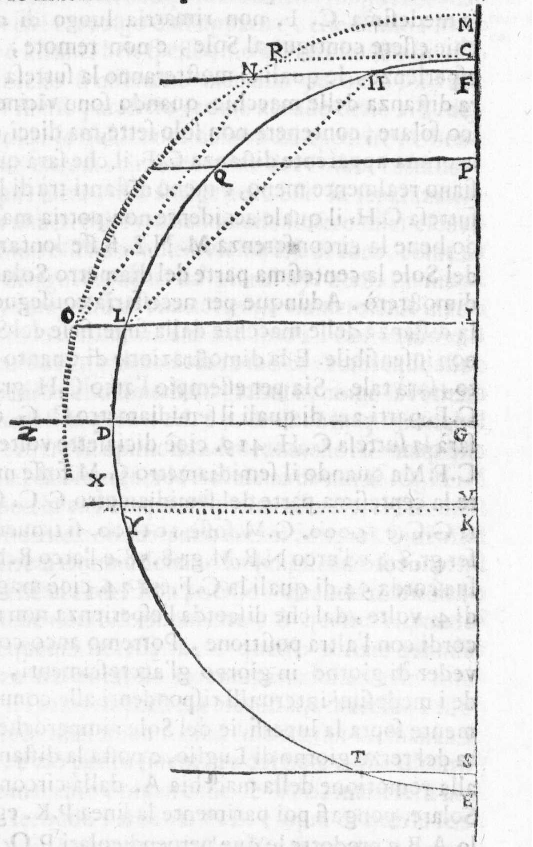
\includegraphics[width=1\textwidth]{ART_Sierotowicz/Sierotowicz_img1-druk.pdf} 
	\caption{Galileo’s Practical Method -- the projection on the observational plane of the segment between two sunspots.}
	\label{sier-fig1}
\end{figure}

\begin{figure}[h]
	\centering
	\includegraphics[width=1\textwidth]{ART_Sierotowicz/Sierotowicz_img2-druk.pdf} 
	\caption{Galileo’s observation on the 1\textsuperscript{st} of July 1613.}
	\label{sier-fig2}
\end{figure}

\begin{figure}[h]
	\centering
	\includegraphics[width=1\textwidth]{ART_Sierotowicz/Sierotowicz_img3-druk.pdf} 
	\caption{Galileo’s observation on the 5\textsuperscript{th} of July 1613.}
	\label{sier-fig3}
\end{figure}

\begin{figure}[h]
	\centering
	\includegraphics[width=1\textwidth]{ART_Sierotowicz/Sierotowicz_img4-druk.pdf} 
	\caption{Sunspots observation, and its geometrical model for the 1\textsuperscript{st} of July 1613. The reconstruction
		by the Author.}
	\label{sier-fig4}
\end{figure}

\begin{figure}[h]
	\centering
	\includegraphics[width=1\textwidth]{ART_Sierotowicz/Sierotowicz_img5-druk.pdf} 
	\caption{Sunspots observation, and its geometrical model for the 5\textsuperscript{th} July. The reconstruction by the
		Author.}
	\label{sier-fig5}
\end{figure}






%\bibitem{camerota_galileo_2004}
%
%\bibitem{camilleri_knowing_2015}
%
%\bibitem{craik_nature_1943}
%
%\bibitem{fantoli_galileo:_2003}
%
%\bibitem{galilei_sunspots_2010}
%
%\bibitem{heilbron_galileo_2010}
%
%\bibitem{nersessian_theoreticians_1992}
%
%\bibitem{nersessian_creating_2008}
%
%\bibitem{palmerino_discussing_2018}
%
%\bibitem{palmieri_mental_2003}
%
%\bibitem{galilei_sunspots_2010-1}
%
%\bibitem{shea_galileo_1970}
%
%\bibitem{sierotowicz_o_2013}
%
%\bibitem{stuart_routledge_2018}
%
%\bibitem{succi_big_2019}
%
%\bibitem{galilei_istoria_1613}
%
%\bibitem{favaro_opere_1895}






\end{artengenv}






%\sekcja{Artykuły}{Articles}





%\sekcja{Z prac Komisji Filozofii Nauk PAU}{Proceedings of the PAU Commission\\\ on the Philosophy of Science}

\begin{artengenv}
	{Łukasz Lamża}
	{How Many Kingdoms of Life? Eukaryotic Phylogeny and Philosophy of Systematics}
	{How Many Kingdoms of Life?\ldots}
	{How Many Kingdoms of Life? Eukaryotic Phylogeny and Philosophy of Systematics}
	{Copernicus Center for Interdisciplinary Studies, Jagiellonian University}
	{According to contemporary understanding of the universal tree of life, the traditionally recognized kingdoms of
		eukaryotic organisms -- Protista, Fungi, Animalia and Plantae -- are irregularly interspersed in a vast phylogenetic
		tree. There are numerous groups that in any Linnaean classification advised by phylogenetic relationships (i.e. a
		Hennigian system) would form sister groups to those kingdoms, therefore requiring us to admit them the same rank. In
		practice, this would lead to the creation of ca. 25-30 new kingdoms that would now be listed among animals and plants
		as ``major types of life''. This poses problems of an aesthetic and educational nature. There are, broadly speaking, two
		ways to deal with that issue: a) ignore the aesthetic and educational arguments and propose classification systems that
		are fully consistent with the Hennigian principles of phylogenetic classification, i.e. are only composed of
		monophyletic taxa; b) ignore Hennigian principles and bunch small, relatively uncharacteristic groups into paraphyletic
		taxa, creating systems that are more convenient. In the paper, I present the debate and analyze the pros and cons of
		both options, briefly commenting on the deeper, third resolution, which would be to abandon classification systems
		entirely. Recent advances in eukaryotic classification and phylogeny are commented in the light of the philosophical
		question of the purpose and design principles of biological classification systems.}
	{taxonomy; systematics; philosophy of biology; eukaryotes; Protista.}



\lettrine[loversize=0.13,lines=2,lraise=-0.05,nindent=0em,findent=0.2pt]%
{E}{}ver since Linnaeus formalized biological classification in his \textit{Systema Naturae}
\parencite{linnaeus_systema_1788},
%\label{ref:RNDRPHrvYOnL2}(Linnaeus, 1788),
there is the unresolved problem of how exactly should new taxa be created,
and, more specifically, into how many subtaxa should higher-rank taxa be split. For instance, is there a convincing
reason why there should be, say, 43 orders of ray-finned fish (class Actinopterygii), but only 3 orders of leeches
(class Hirudinea)? Are there any objective arguments for one arrangement over another, or is it purely a matter of
taste? There is a considerable body of work in philosophy of biology that discusses such issues
(see \cite{hull_effect_1965,hull_contemporary_1970,schuh_biological_2011} and especially \cite{mayr_classifications_2002}).
%\label{ref:RNDfhQVj97gMS}(see Hull, 1965, 1970; Schuh and Brower, 2011; and especially Mayr and Bock, 2002).

While ongoing changes at lower ranks (i.e. species, genus, family and order) are of high importance to specialists, the
public is much more likely to encounter changes at the higher ranks (from class up). Of special importance is the
traditionally highest category of kingdom (now partially superseded by domain -- see below) which delineates major
``types of life'' and is of enormous educational and heuristic value
\parencite{copeland_kingdoms_1938,cavalier-smith_eukaryote_1981}.
%\label{ref:RND3zNGphpm9n}(Copeland, 1938; Cavalier-Smith, 1981).
For centuries there has been slow incremental change in the classification of life at the level
of kingdom. In the recent two decades, however, the rapidly increasing knowledge of the general topology of the
universal tree of life, lead to the realization that traditionally distinguished kingdoms are interspersed in a thick
``bush'' of major branches
\parencite[see e.g.][]{baldauf_kingdom-level_2000}.
%\label{ref:RNDASUVezikg7}(see e.g. Baldauf et al., 2000).
In this paper, I wish to analyze
this situation, with special attention to the structure of the eukaryotic tree of life. 

\section{The rank of kingdom}

In biological systematics, starting from Linnaeus, the rank of kingdom has long been the highest of all taxonomic ranks.
In Linnaeus’ \textit{Systema Naturae}, there were 3 of them -- the animal, plant and mineral kingdom
\parencite{linnaeus_systema_1788},
%\label{ref:RND6bXO1caZ3A}(Linnaeus, 1788),
and the division of all living things into two kingdoms was retained in
biology for a long time. Only recently the even higher rank of domain was introduced by Carl Woese
\parencite{woese_towards_1990},
%\label{ref:RNDDiuS3oKKqs}(Woese, Kandler and Wheelis, 1990),
who intended to accentuate the special character of
Archaea, famously identified by him and George Fox
\parencite{woese_phylogenetic_1977}
%\label{ref:RNDIQY6gpSHPx}(Woese and Fox, 1977)
to be fundamentally
different from both bacteria and eukaryotes; although it has been recently suggested that eukaryotes actually evolved
from archaea
\parencite{williams_archaeal_2013}.
%\label{ref:RND5ULE3HHm08}(Williams et al., 2013).
Even in Woese’s 1990 revision, however, three ``primary
kingdoms'' were named with the idea that the rank of kingdom remains the basic level at which major ``types of life'' are
to be identified.

The number of the kingdoms of life discerned by biologists changes through time rather slowly. A contemporary student of
both introductory and advanced biological texts is almost certain to encounter the following:

\begin{itemize}
\item either a single kingdom of bacteria, variously called Prokaryotae, Bacteria or Monera, or, in a more modern
variation, two kingdoms: the so-called true bacteria (Eubacteria, sometimes Bacteria) and the archaeans (Archaea,
sometimes Archaebacteria);
\item the single kingdom of protists (usually Protista or Protoctista), which encompasses all eukaryotes not belonging
to the three multicellular kingdoms (see below); in some modern sources
\parencite{ruggiero_higher_2015}
%\label{ref:RNDdqkS30YvK5}(e.g. Ruggiero et al., 2015)
there is a separate kingdom Chromista encompassing a large monophyletic subgroup of protists, including brown
algae which are large, multicellular and quite complex;
\item the three multicellular eukaryotic kingdoms: plants (Plantae, sometimes Viridiplantae), animals (Animalia,
sometimes Metazoa) and fungi (Fungi, sometimes Mycota). 
\end{itemize}
Note that the list is quite conservative, but the number of kingdoms slowly increases. Plants and  animals are the two
original Linnaean kingdoms of life. Protists were argued to be a separate kingdom by Ernst Haeckel in 1866
\parencite{haeckel_generelle_1866}.
%\label{ref:RNDnC4UhA8FAD}(Haeckel, 1866).
Bacteria were given a separate kingdom in 1938
\parencite{copeland_kingdoms_1938}
%\label{ref:RNDsDaQPHVHjj}(Copeland, 1938)
and, interestingly, the fungi have been proposed as a kingdom separate from
plants only in 1969
\parencite{whittaker_new_1969}.
%\label{ref:RNDzC4ki5UDBu}(Whittaker, 1969).
The distinct kingdom for Archaea, as mentioned, was
proposed in 1977 and Thomas Cavalier-Smith first proposed elevating Chromista to the rank of kingdom in 1981
\parencite{cavalier-smith_eukaryote_1981}.
%\label{ref:RNDnKGExfa2wY}(Cavalier-Smith, 1981). 

Arguably, the most common variant found in introductory texts is the one with five kingdoms: Bacteria, Protoctista,
Plantae, Animalia, Fungi, and this very division has been employed in the highly influential popular book by Lynn
Margulis and Michael Chapman, \textit{Kingdoms and Domains}
\parencite{margulis_kingdoms_2009},
%\label{ref:RND5xqZMYPEO1}(Margulis and Chapman, 2009),
which has become an authoritative source on biological megasystematics. In a recent proposal of a comprehensive
classification of life, down to the level of order
\parencite{ruggiero_higher_2015},
%\label{ref:RNDva9PR88ZHQ}(Ruggiero et al., 2015),
there are seven
kingdoms: Archaea/Archaebacteria, Bacteria/Eubacteria, Protozoa, Chromista, Fungi, Plantae and Animalia. This proposal
is a consensus view of over 3000 taxonomists (!) and is likely to become the standard point of reference for
professional biologists for years to come, even though it has been criticized, especially with regard to specific
taxonomic decisions
\parencite[e.g.][]{tedersoo_high-level_2018}.
%\label{ref:RND4kurLEBPnA}(e.g. Tedersoo et al., 2018).

All in all, based on that quick review, it may seem that a general view of the diversity of life, and its representation
in biological taxonomy, is now more or less understood, and major changes to the number of kingdom occur rarely. In
reality, it not that simple. In the past decades there has been considerable controversy surrounding the number and
identity of the highest ranks in systematics, and the summary presented above might be termed the ``conservative view''
by some. In fact, there are sources claiming that 11-12 prokaryotic kingdoms
\parencite{petitjean_rooting_2014}
%\label{ref:RNDXxF0Lm1b0k}(Petitjean et al., 2014)
and 20-27 eukaryotic kingdoms
\parencite{pawlowski_new_2013,tedersoo_proposal_2017}
%\label{ref:RNDB4YmCpjg7j}(Pawlowski, 2013; Tedersoo, 2017)
should be
distinguished.

The purpose of the present paper is to identify the cause of that confusion and its possible resolutions, using mostly
examples related to the eukaryotic tree of life.

\section{Paraphyletic taxa and classification systems}

Starting from Darwin himself, it has become increasingly clear that biological systematics must somehow portray
evolutionary patterns. This was formalized in Willi Hennig’s \textit{Phylogenetic Systematics}
\parencite{hennig_phylogenetic_1966}
%\label{ref:RNDWJhbleZaU4}(Hennig, 1966)
where the now-ubiquitous concepts of symplesiomorphy, synapomorphy and
convergence, and the corresponding types of taxa -- paraphyletic, monophyletic and polyphyletic -- were formalized.
Hennig forcefully argued that valid taxa should only be monophyletic groups, i.e. (true) clades, that is groups of
species composed of \textit{all} descendants of a given species, possessing a common derivative character
(synapomorphy). In the science of cladistics this has since become gospel.

While admirable, this prescription leads to ``taxonomical inflation'' as more and more taxa are identified. Before we
illustrate it with an example relevant for the present study, let’s consider a case with more familiar taxa.

Vertebrates (subphylum Vertebrata of phylum Chordata) are divided into a number of classes. A popular list of vertebrate
classes that you may hear even from a child (the specific reason for mentioning children in this context will be given
below) is as follows: fish, amphibians, reptiles, birds and mammals. A better-educated person might cite the current
scientific consensus that ``fish'' should be actually split into a number of separate classes: hagfish (Myxini), lampreys
(Hyperoartia), cartilaginous fish (Chondrichthyes), ray-finned fish (Actinopterygii) and lobe-finned fish
(Sarcopterygii), the reason being that ``fish'' is actually a paraphyletic grouping. This prescription to discuss five
types of fish, which a layperson may identify as unnecessary and confusing (why five classes of fish and just one class
of birds?), is a first sign of what happens when one attempts to divide a given taxon into monophyletic subtaxa.

If one were to portray the abovementioned vertebrate classes on a phylogenetic tree, something like Fig. 1 might be a
reasonable representation of actual relationships.

\begin{figure}[h]
	\centering
	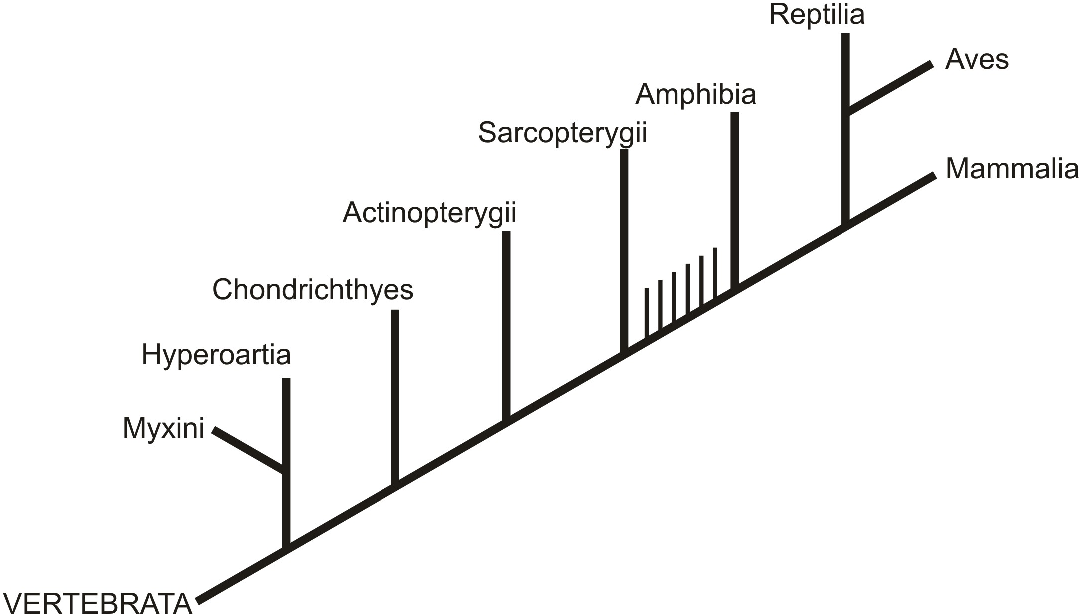
\includegraphics[width=1\textwidth]{PAU_Lamza/Lamzaorg-img001.pdf}
	\caption{A highly simplified, and ultimately wrong, phylogenetic tree of extant vertebrates that attempts to
		include only the extant classes of subphylum Vertebrata. The ‘comb’ represents the area magnified in Fig. 2. It is
		clear that one cannot map a ranked classification of extant vertebrate classes onto a valid phylogenetic tree,
		especially because of the existence of extinct groups. Specifically, it is impossible to validly represent the actual
		relationships between (paraphyletic and now obsolete) Reptilia and Aves (which nest within reptiles).}
	%\label{lamza-fig1}
\end{figure}

This is, however, yet another simplification. A more careful analysis of \textit{any }segment of the vertebrate
phylogenetic tree will reveal that in between the well-known groups there are numerous groups, usually extinct, that
would all require classes of their own, if the bordering taxa are given the rank of class -- consult Fig. 2.

\begin{figure}[h]
	\centering
	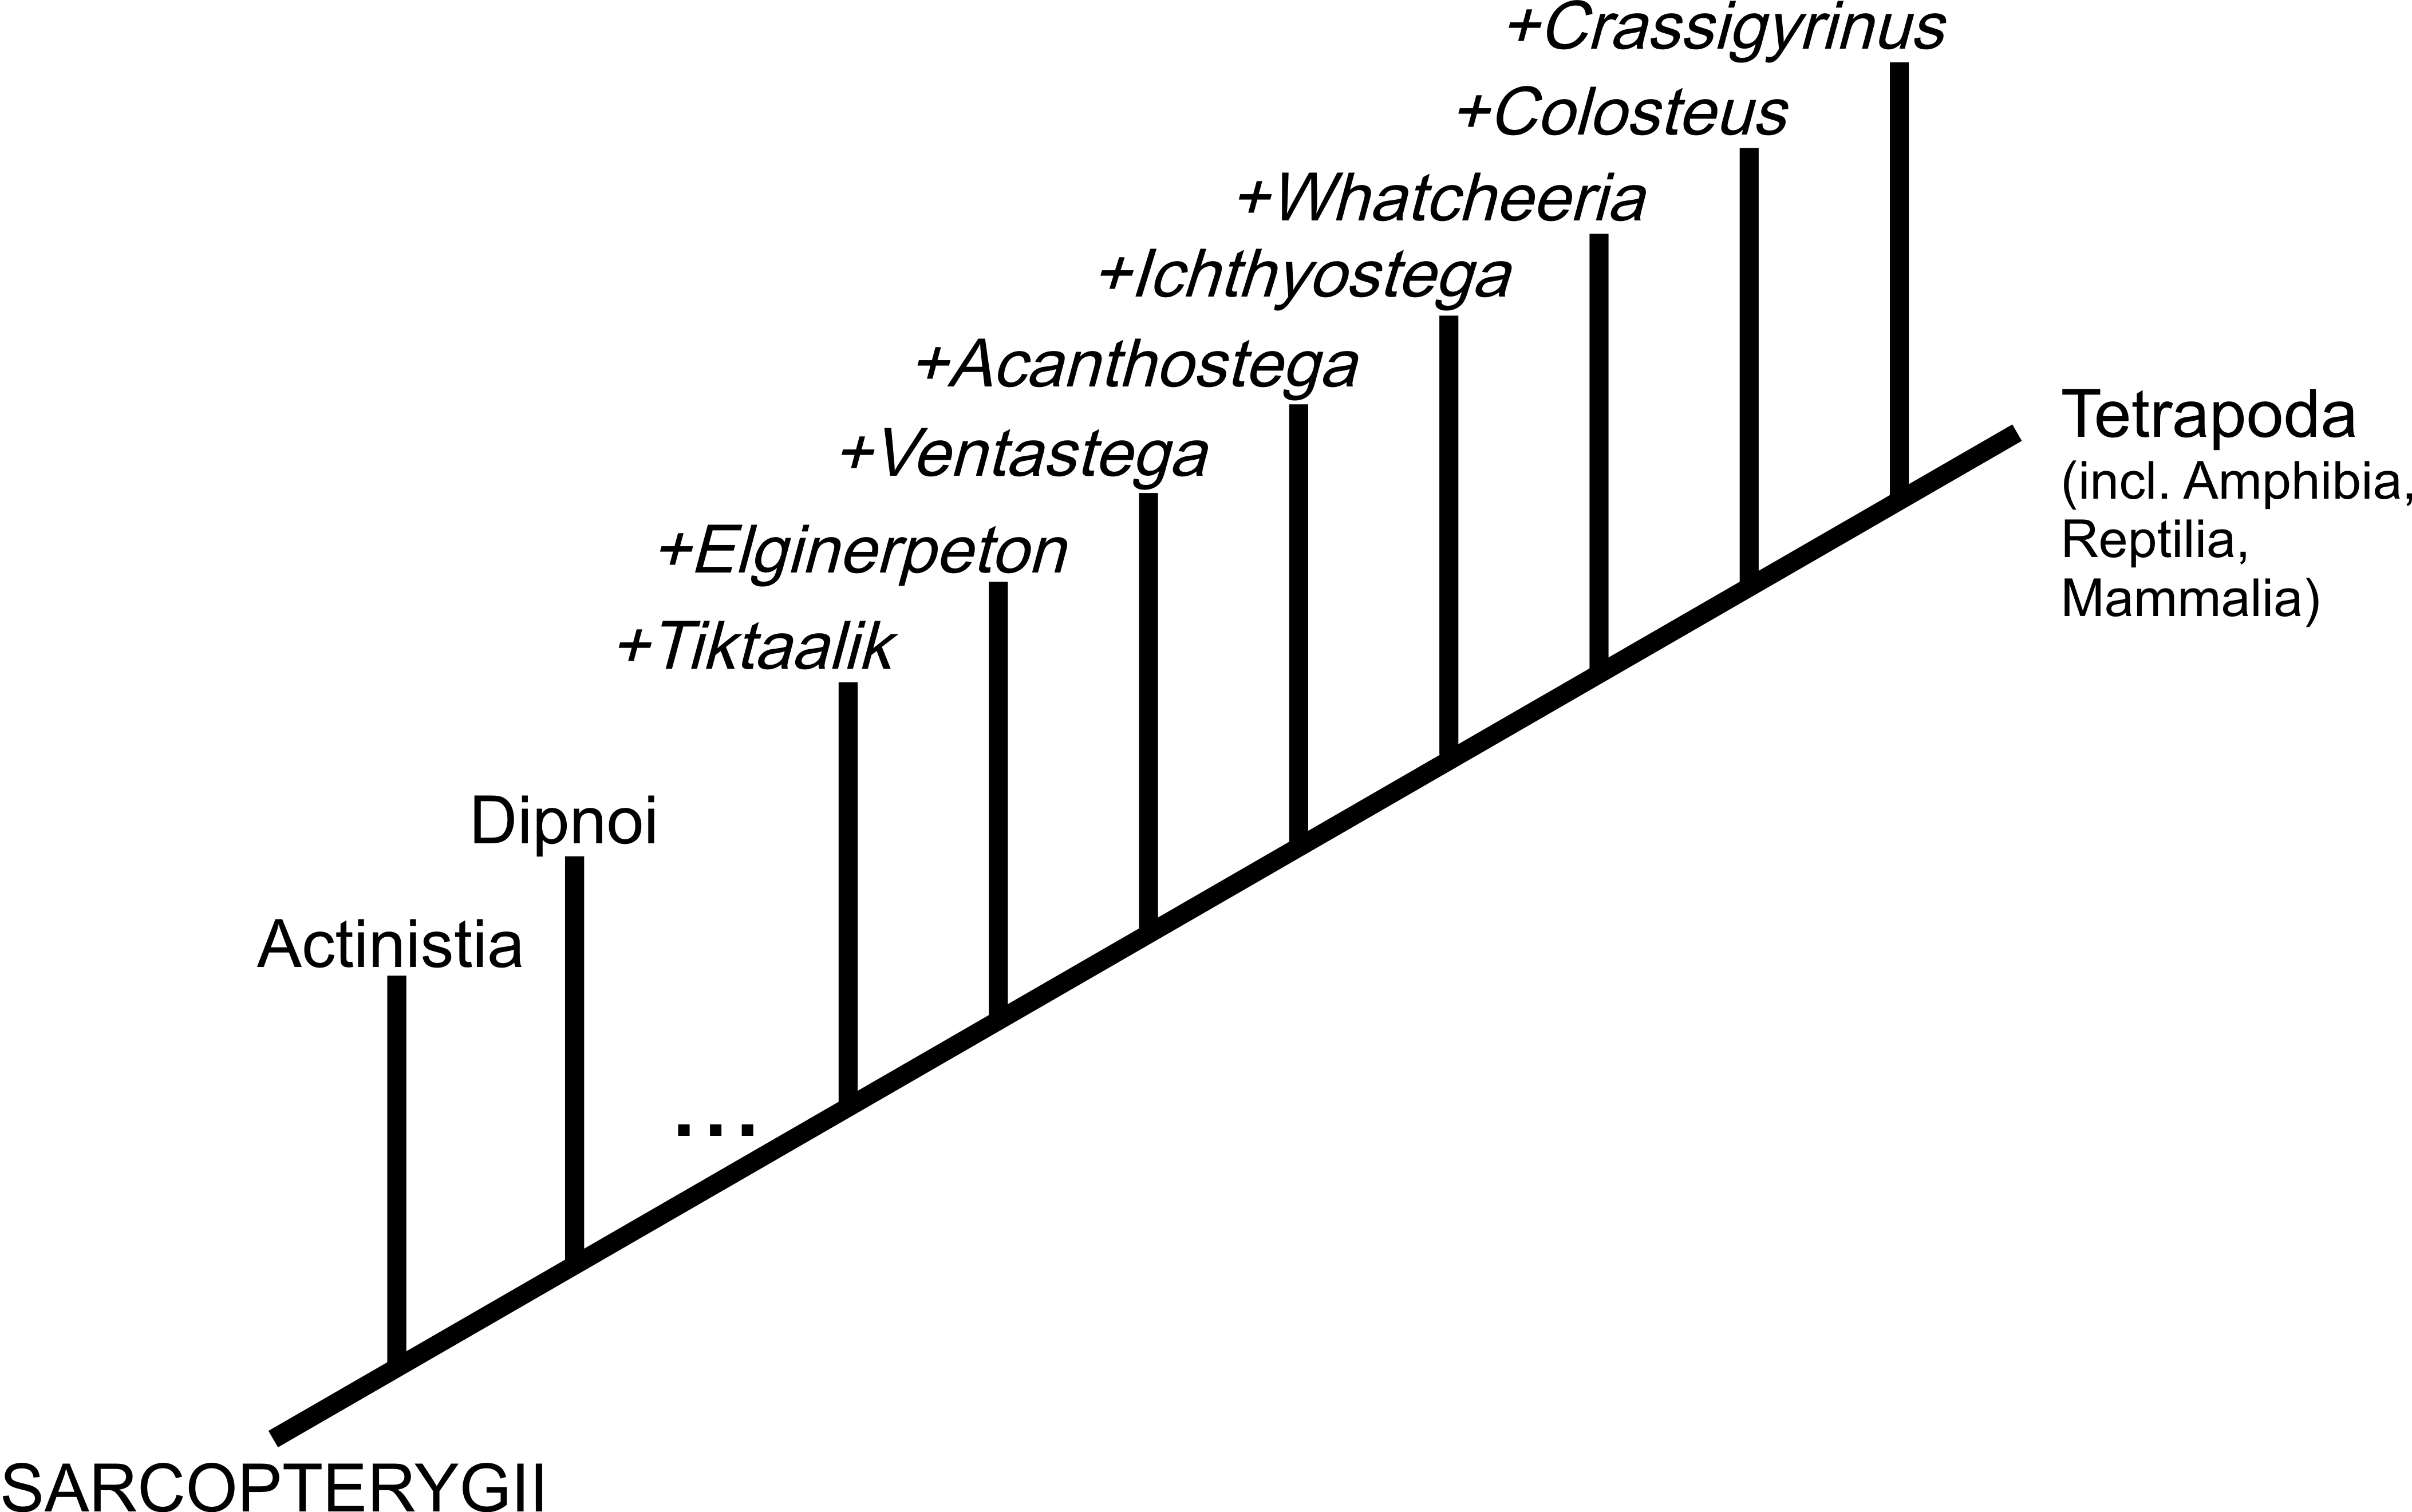
\includegraphics[width=1\textwidth]{PAU_Lamza/Lamzaorg-img002.jpg}
	\caption{A slightly more realistic representation of a segment of the vertebrate phylogenetic tree, based on
		\parencite{swartz_marine_2012}
		%\label{ref:RNDPuknxVrJnD}(Swartz, 2012)
		(with many taxa removed, most notably a large group of early sarcopterygians,
		denoted by an ellipsis). The improvement over Fig. 1 is mostly in that: a) the term Sarcopterygii is now correctly
		represented to also include all tetrapods, while in common usage, represented in Fig. 1, it refers only to coelacanths
		(which belong to Actinistia) and lungfish (which belong to Dipnoi); b) a number of extinct (marked by a cross) genera
		are presented.}
	%\label{lamza-fig2}
\end{figure}

It is clear that in order to divide the taxa listed in Fig. 2 into classes, one would have to give each genus presented
in that figure its own high-level taxon (here: most likely class). The alternative is accepting paraphyletic taxa, for
instance by grouping all stem tetrapods (Tiktaalik\ldots Crassigyrinus) in a single class. It clearly goes against
phylogenetic systematics, which is usually defended by biologists working with specific groups of organisms as the only
method of creating taxonomies that is commensurate with the theory of evolution
\parencite[see e.g.][]{williams_pursuit_2007}
%\label{ref:RNDkC4ruFguZT}(see e.g. Williams and Kociolek, 2007).

There are ways to avoid that, one of which is the so-called sequencing convention proposed by Nelson
\parencite*{nelson_phylogenetic_1972}
%\label{ref:RNDHQubFlpSOG}(1972)
and developed by Wiley
\parencite*{wiley_phylogenetics:_1981}
%\label{ref:RNDoeFoXTp1sn}(1981)
and others, which partly
automates the ranking process in various branches of the phylogenetic tree. But for new, let’s assume that we want to
hold on to strict Hennigian principles; what would be the consequences? Quite simple: the necessity to create a
complete system of monophyletic taxa, in case of vertebrates, would lead to the erection of tens, if not hundreds,
classes of vertebrates which defeats the simplifying purpose of classification. Another solution would be to erect a
large number of taxa of intermediate rank -- this has been done, for example, by McKenna \& Bell in their influential
classification of mammals
\parencite{mckenna_classification_1997}:
%\label{ref:RNDTh5Uw8JZAm}(McKenna and Bell, 1997):

\begin{longitemize}
\item class Mammalia
\begin{longitemize}
\item subclass Prototheria
\item subclass Theriiformes
\begin{longitemize}
\item infraclass +Allotheria
\item infraclass +Eutriconodonta
\item infraclass Holotheria
\begin{longitemize}
\item superlegion +Kuehneotheria
\item superlegion Trechnotheria
\begin{longitemize}
\item legion +Symmetrodonta
\item legion Cladotheria
\begin{longitemize}
\item sublegion +Dryolestoidea
\item sublegion Zatheria
\begin{longitemize}
\item infralegion +Peramura
\item infralegion Tribosphenida
\item \ldots
\end{longitemize}
\end{longitemize}
\end{longitemize}
\end{longitemize}
\end{longitemize}
\end{longitemize}
\end{longitemize}

It is worth noting that the authors of that classification are paleontologists and their system is clearly intended as
an answer to the problem of finding a proper taxonomic space for extinct groups. As a result, a staggering number of
ranks were created. In ``core Linnaean'' taxonomy classes are composed of orders, i.e. class and order are neighboring
ranks. In McKenna \& Bell’s system one will find between them: subclasses, infraclasses, superlegions, legions,
sublegions, infralegions, supercohorts, cohorts, magnorders, superorders, grandorders and mirorders. The term
``taxonomic inflation'' may thus have two meanings: the creation of an impractically large number of equally-ranked taxa
and the creation of an impractically large number of ranks.

Let’s now discuss these two alternatives in more detail.

\section{The solutions}
\vspace*{-1cm}
\subsection{Solution I: classifications with only monophyletic taxa}

As mentioned above, strictly adhering to Hennig’s prescription to accept only monophyletic taxa leads to ``taxonomic
inflation'' -- which seems to go against the aesthetic intuition of those biologists who dread the idea of splitting a
given, let’s say, phylum, into 50 classes
\parencite{cavalier-smith_revised_1998}.
%\label{ref:RNDsx8NDQDrK2}(Cavalier-Smith, 1998).

Surprisingly, the solution that has been commonly employed is to do something perhaps even more drastic: to drop
altogether the Linnaean ``logic'' of classification which is based on the simple idea that taxa of a given rank are
divided into a number of subordinate taxa of the same lower rank -- i.e. kingdoms are divided \textit{only} into phyla;
phyla are divided \textit{only} into classes; classes \textit{only} into orders etc. In other words, every order
belonging to a given phylum must \textit{also }belong to a certain class (or, in some cases, be included as
\textit{incertae sedis}, i.e. temporarily awaiting class attribution). In many modern classifications, however, there
are \textit{missing ranks}. As an example, consider the classification of vertebrates presented by the eminent
paleontologist Michael Benton in his \textit{Vertebrate Palaeontology}
\parencite[p.433nn]{benton_vertebrate_2014}
%\label{ref:RNDqnkTfPlTq8}(Benton, 2014, p.433nn):

\pagebreak%tu
\noindent$\bullet$ superclass Tetrapoda:
\begin{addmargin}[1em]{0em}
 $\circ$ family Elginerpetontidae\\
 $\circ$ \textit{Ventastega}\\
 $\circ$ \textit{Acanthostega}\\
 $\circ$ \textit{Ichthyostega}\\
 $\circ$ \textit{Tulerpeton}\\
 $\circ$ family Colosteidae\\
 $\circ$ family Crassigyrinidae\\
 $\circ$ family Whatcheeriidae\\
 $\circ$ family Baphetidae\\
 $\circ$ class Neotetrapoda [where amphibians, reptiles, birds and mammals can be found -- L.L.]
\end{addmargin}

This is a remarkable solution. Note that it clearly opposes the centuries-old tradition, formalized by Linnaeus, to
create consistent, complete hierarchies. Here we have a superclass that is composed of a single class, 5 families and 4
genera.

The missing ranks may look unsettling at first, but this convention is quickly gaining popularity, as it seems to offer
a welcome rescue from the otherwise inescapable alternatives discussed in the previous paragraph. A recent
classification of eukaryotes, published first in 2005
\parencite{adl_new_2005},
%\label{ref:RND5C0kzbt9Jm}(Adl et al., 2005),
then in a revised
form in 2012
\parencite{adl_revised_2012},
%\label{ref:RND2nC4dhq2C7}(Adl et al., 2012),
employs precisely that methodology. Note that this is an
extremely well-respected classification, created by a consortium that includes world-class experts in eukaryotic
diversity (such as Alastair Simpson or Sergei Karpov). The pair of papers is now amongst the most oft-quoted articles
in the field, which means in practice that it is now a point of departure in any discussion of eukaryote
classification.

In both papers the ranks are altogether dropped. Curiously, the taxa are presented in a semi-ordered hierarchical form
where subordinate taxa are given more black dots. For instance, in the earlier paper
\parencite{adl_new_2005}
%\label{ref:RNDFR1OTfHJvd}(Adl et al., 2005)
the group Opisthokonta is presented as follows (numerous taxa have been omitted):

\noindent OPISTHOKONTA\\
$\bullet$ Fungi\\
$\bullet\bullet$ Basidiomycota\\
$\bullet\bullet$ Urediniomycetes\\
$\bullet\bullet$ Ustilaginomycetes\\
$\bullet\bullet$ Ascomycota\\
$\bullet\bullet$$\bullet$ \textit{Neolecta}\\
$\bullet\bullet$$\bullet$ Taphrinomycotina\\
\ldots\\
$\bullet$ Mesomycetozoa\\
$\bullet\bullet$ Aphelidea\\
$\bullet\bullet$ \textit{Corallochytrium}\\
$\bullet\bullet$ \textit{Capsaspora}\\
$\bullet\bullet$ Ichthyosporea\\
$\bullet\bullet$ \textit{Ministeria}\\
$\bullet\bullet$ Nucleariida\\
$\bullet$ Choanomonada\\
$\bullet$ Metazoa\\
$\bullet\bullet$ Porifera\\
$\bullet\bullet$$\bullet$ Silicispongia\\
$\bullet\bullet$$\bullet\bullet$ Hexactinellida\\
$\bullet\bullet$$\bullet\bullet$ Demospongiae (\ldots)

Let’s note a few properties of this classification method. First of all, the four main groups of Opisthokonta
(the ones with a single dot, i.e. fungi, mesomycetozoans, choanomonads and animals) are, to the best of current
phylogenetic knowledge, monophyletic. This makes them perfect for the role of taxa in an openly Linnaean system, that
is at the same time in line with Hennig’s rules of phylogenetic classification. The taxa with the same number of dots,
however, represent radically different ranks in previously published classifications. The group Mesomycetozoa, as
presented here, is composed of three genera (\textit{Corallochytrium}, \textit{Capsaspora} and \textit{Ministeria}),
two classes (Aphelidea and Ichthyosporea) and one order (Nucleariida). One might of course erect classes for all of
them, which however, often leads to taxonomic inflation, as mentioned in the previous section.

Let’s now specifically discuss the problem of kingdoms. If we hold on to the idea that equal ``ranks'' in the
classification by Adl \textit{et al.} should be given equal Linnaean ranks, we would be forced to create two additional
kingdoms Choanomonada and Mesomycetozoa, that would be placed alongside Fungi and Metazoa/Animalia in the, most likely,
superkingdom Opisthokonta (plus other kingdoms in other superkingdoms). That is, in fact, a fairly popular point of
view, expressed for instance by Tedersoo
\parencite*{tedersoo_proposal_2017},
%\label{ref:RNDXAoIqIPayD}(2017),
who includes kingdoms Choanoflagellozoa
(essentially synonymous with Adl \textit{et al.}’s Choanomonada) and Ichthyosporia (Ichthyosporea is a synonym of
Mesomycetozoa in many classification systems). It is worth noting that Tedersoo’s system might be thought of as a good
demonstration of what happens if one attempts to create a Linnaean system adhering to Hennigian constraints, based on
modern understanding of eukaryotic phylogeny (the classification by Adl \textit{et al.} is listed by Tedersoo as one of
his main sources of information). The result? His system has 32 eukaryotic kingdoms. Let’s cite his own opinion on that
fact: ``In the proposed classification, the erection of 32 eukaryote kingdoms certainly catches and, perhaps, scratches
the eye. I found adoption of multiple kingdoms necessary to follow the monophyly principle […].''
\parencite[p.8]{tedersoo_proposal_2017}
%\label{ref:RNDP7J0D4JTk6}(Tedersoo, 2017, p.8)

Note that Adl \textit{et al. }themselves stand \textit{against }such practices, calling such artificially created
higher-level taxa ``superfluous''
\parencite[p.430]{adl_revised_2012},
%\label{ref:RNDTkKC0gomXM}(Adl et al., 2012, p.430),
therefore openly arguing for
classification with missing taxa.

\subsection{Solution II: classifications with paraphyletic taxa}

The most vocal contemporary proponent of that solution is probably Thomas Cavalier-Smith, a controversial figure among
microbiologists, who, however, is at the same time undoubtedly one of the most influential personas in the field of
eukaryotic systematics. His contributions include the early recognition, and naming, of Excavata, Opisthokonta,
Rhizaria and Chromista -- all of them being now largely accepted, and the latter three: most likely monophyletic,
mega-grouping of eukaryotes. In his proposed classification of life (with six kingdoms)
\parencite{cavalier-smith_revised_1998}
%\label{ref:RNDScaXMIFqT5}(Cavalier-Smith, 1998)
there is a long section on ``philosophical preliminaries'', where the
necessity for admitting paraphyletic taxa is forcefully defended. His two main arguments against the Hennigian
requirement to limit taxa to clades are as follows:

1) It leads to instability. Each new discovery in biology -- be it a paleontological or molecular novelty, or simply the
discovery of a new species or a reinterpretation of anatomical data -- may lead to the reassessment of a monophyletic
taxon as paraphyletic, which would force the biologists to update classification systems. In practice it would mean
hundreds, if not thousands, of revisions every year.

2) It is not practical. Let’s quote Cavalier-Smith himself: ``Whether a taxon is paraphyletic or not is irrelevant to its
validity as a taxon. It is also irrelevant to many of the uses to which classifications are put, such as arranging
specimens in a museum, organising the chapters in a biology textbook, or providing a convenient label, e.g. bacteria or
fungi, for a group of similar organisms.''
\parencite[p.212]{cavalier-smith_revised_1998}
%\label{ref:RNDUlTuwI9YEO}(Cavalier-Smith, 1998, p.212)

As a result, Cavalier-Smith for about two decades has become an active opponent of Hennigian classification, especially
in the field of microbiology. Every year or two he proposes a new system of classification, sometimes general, most
often specific to a group of eukaryotes
\parencite{cavalier-smith_phagotrophic_2002,cavalier-smith_early_2013,cavalier-smith_higher_2016},
%\label{ref:RNDtoAIslWhri}(see e.g. Cavalier-Smith, 2002, 2013, 2016),
usually
being a carefully crafted compromise between contemporary phylogenetic knowledge and practicality. His 1998 system
\parencite{cavalier-smith_revised_1998}
%\label{ref:RNDJbJ6dU4tG1}(Cavalier-Smith, 1998)
has six kingdoms:

\begin{longitemize}
\item empire/superkingdom Prokaryota*
\begin{longitemize}
\item kingdom Bacteria* [note: Archaebacteria are to be found here, as an infrakingdom]
\end{longitemize}
\item empire/superkingdom Eukaryota
\begin{longitemize}
\item kingdom Protozoa*
\begin{longitemize}
\item subkingdom Archezoa*
\item subkingdom Neozoa*
\end{longitemize}
\item kingdom Animalia
\item kingdom Fungi
\item kingdom Plantae
\item kingdom Chromista
\end{longitemize}
\end{longitemize}
All openly paraphyletic (``almost certainly paraphyletic'' in his own words) taxa are marked with an asterisk. It is
interesting to note that, while Cavalier-Smith openly opposes Hennigian phylogenetic systematics, his ``illegal''
taxonomies are highly popular. A quick look into any contemporary paper on eukaryotic systematics will reveal a number
of high-level taxa formally defined by Cavalier-Smith, many of them known or suspected to be paraphyletic. The reason
is simple: his classifications are extremely convenient, because they are invariably composed in such a way as to
include only a minimal number of taxa \textit{and} ranks which are \textit{usually }monophyletic, but sometimes are
paraphyletic if that makes for a convenient system. The reader is referred to the above-cited paper (Cavalier-Smith,
1998) where his philosophy of biological classification is explained in detail.

On a side, and probably more personal, note: the zoologists reading this paper may find it interesting to go through his
proposed classification of the animal kingdom
\parencite[pp.235–237]{cavalier-smith_revised_1998}
%\label{ref:RNDayLTgHPurs}(Cavalier-Smith, 1998, pp.235–237)
which offers,
in the opinion of the author of this paper, a refreshing look at the list of animal phyla. As currently recognized,
there is somewhere around 30-35 phyla -- consult any modern textbook on zoology -- that only recently began to be grouped
into a few large monophyletic groups, such as Spiralia, Ecdysozoa or Deuterostomia. Other than that, there is a
confusing diversity of tiny phyla, most of them unknown to the general public: how many non-zoologists know of
Kinorhyncha, Loricifera, Gnathostomulida (jaw worms) or Acanthocephala (spiny-headed worms)? Cavalier-Smith groups all
animals into 22 phyla -- still a long list, but, especially with the aid of his clear, succinct diagnoses, is much more
manageable. The classification includes some, but rather few, paraphyletic taxa.

\subsection{Solution III: abandon classification systems}

The third solution would be to run away from the problem, so to speak, and refrain from explicitly writing down
classifications, and discuss biological diversity through phylogenetic trees only. This has been proposed from time to
time by certain scientists and philosophers (the proposal has been reviewed and critiqued by Michael Benton
\parencite*{benton_stems_2000}).
%\label{ref:RNDvl4WtKWtke}(2000)).
While reading biological literature, one finds this sentiment expressed from time to
time, especially by specialists working with rapidly changing classification systems. There is a fascinating, heated
dialogue that ensued during the 1970 First International Conference on Ephemeroptera, recorded in this conference’s
proceedings
\parencite[pp.151–154]{peters_proceedings_1973},
%\label{ref:RNDKBHKSFREeT}(Peters and Peters, 1973, pp.151–154),
where a group of entomologists become
increasingly frustrated by their inability to create a classification system based on the otherwise clear phylogenetic
evidence presented by one of the participants
\parencite{edmunds_jr_critical_1973}.
%\label{ref:RNDRwD3oy2Fl1}(Edmunds Jr, 1973).
In fact, all the problems
discussed in this paper with regard to higher ranks are mentioned during that discussion, which is about families,
subfamilies and genera of Ephemeroptera, which makes for a great read.

There are at least two large groups in biology that have abandoned updating the classification of the organisms they are
working with: botanists working with flowering plants and malacologists.

In the first case, one would be hard-pressed to find a recent authoritative classification of flowering plants, because
the focus of the communal effort has long been the creation of better and better phylogenies, not taxonomies. The
Angiosperm Phylogeny Group regularly publishes the new view on plant phylogeny, employing formal taxa only to the level
of order %\label{ref:RNDly7gwmyvG1}(see e.g. Chase et al., 2016). All the higher-rank taxa are abandoned, and no
higher-rank taxonomies are officially accepted by APG.

The exactly same process had happened in the field of malacology, where for years there were no formal definitions of
gastropod taxa above the level of superfamily
\parencite[see][]{bouchet_classification_2005}.
%\label{ref:RND5saL769IKK}(see Bouchet and Rocroi, 2005).
Interestingly,
the situation visibly upset some of the workers in the field who started spontaneously grouping the newly defined
families and superfamilies into orders, those into superorders, subclasses etc. Last year in a revision of the 2005
classification
\parencite{bouchet_revised_2017},
%\label{ref:RNDSnxh8fRQNP}(Bouchet et al., 2017),
the authors surrendered and included higher-ranked
taxa, although the system is now very ``messy'': it includes numerous intermediate-level ranks that correspond to the
unranked clades in the previous classification -- there are classes, subclasses, infraclasses, cohorts, subcohorts,
superorders, orders, suborders and infraorders in the system, plus a handful of openly paraphyletic ``grades''. The
struggle of malacologists to bring back Linnaean classification into the world of Hennigian unranked lists à la Adl
\textit{et al.} leads to exactly the same problems that were discussed in the previous sections.

The case of gastropod classification illustrates, however, that even specialists working in very narrow fields need
balanced ranked classification systems. It is not only for the purposes of educating the young, writing books or
organizing museum expositions that we need neat, logical classifications with no missing ranks and a small number of
distinctive, easy to remember taxa. The specialists need them too. The option to abandon classification systems seems
to be not viable, especially that it is both trivial and tempting to create a list of clades from a phylogenetic tree,
adding ranks to some or all taxa, which would be a \textit{de facto} classification, just like Benton did in his
\textit{Vertebrate Palaeontology}.

\section{Summary}

Our increasing knowledge of biodiversity, especially in the case of microbiology, both prokaryotic and eukaryotic, will
inevitably lead to the escalation of the problems presented in this paper. Because it doesn’t seem plausible that
classification systems will be altogether abandoned (which would leave us only with phylogenetic trees, sometimes
presented as unranked lists), it seems that we must somehow solve the problem of creating classification systems in the
times of abundant phylogenetic data.

Broadly speaking, there seem to be two directions that one might take: 1) to follow phylogenetic data to the letter; 2)
to follow intuition and convenience. Simply put, the option 1) would mean having only proper monophyletic taxa, but a
highly impractical system; and the option 2) would mean having also paraphyletic taxa \textit{and} a system that is
practical.

In the special case of eukaryotic kingdoms, the first route would lead to a revolution in biological classification of
life and numerous kingdoms currently unknown to the general public would be introduced
\parencite{tedersoo_proposal_2017},
%\label{ref:RND3uML7k6B2X}(Tedersoo, 2017),
such as Oxymonada, Breviatea or Filasteriae, that would now be listed
alongside plants, animals and fungi as ``major types of life''. Alternatively, one might drop the traditional kingdoms
altogether and define the currently recognized eukaryotic ``supergroups''
\parencite[e.g.][]{keeling_tree_2005}
%\label{ref:RNDsc7VI9vP7w}(e.g. Keeling et al., 2005)
as kingdoms, and what we know recognize as kingdoms would have to be downranked into subkingdoms or
``microkingdoms''
\parencite{pawlowski_new_2013}.
%\label{ref:RNDAlF3xlGnxL}(Pawlowski, 2013).
This would be the resulting classification:

\begin{itemize}
\item kingdom Excavata
\item kingdom Amoebozoa
\item kingdom Opisthokonta (incl. fungi and animals)
\item kingdom Archaeplastida (incl. plants)
\item kingdom Rhizaria
\item kingdom Alveolata
\item kingdom Heterokonta
\end{itemize}
Obviously, this would \textit{not} solve the problem, if one would stubbornly keep on sticking to Hennigian rules. First
of all, Excavata may be paraphyletic
\parencite{he_alternative_2014},
%\label{ref:RNDd85mwMFAal}(He et al., 2014),
in which case we would have to split
it into monophyletic groups, resulting in a classification system alike to this:

\begin{itemize}
\item kingdom Euglenozoa (former Excavata)
\item kingdom Heterolobosea (former Excavata)
\item kingdom Jakobea (former Excavata)
\item kingdom Metamonada (former Excavata)
\item kingdom Amoebozoa
\item kingdom Opisthokonta (incl. fungi and animals)
\item kingdom Archaeplastida (incl. plants)
\item kingdom Rhizaria
\item kingdom Alveolata
\item kingdom Heterokonta
\end{itemize}
Secondly, there is at least a dozen groups of eukaryotes that don’t fit neatly into any of the supergroups, including
\textit{Tsukubamonas} and \textit{Malawimonas}, Cavalier-Smith’s Varisulca, Apusozoa, but also much better-known groups
such as Cryptophyta or Haptophyta. Consequently, in Tedersoo’s system, there \textit{are} kingdoms Malawimonada,
Tsukubamonada, Apusozoa, Cryptista and Haptista which brings us to square one. Obviously, replacing traditional
kingdoms with eukaryotic supergroups is \textit{not }a solution.

The second option -- to retain the general structure of the present classification of life into kingdoms -- is not fully
satisfactory, either, because the old kingdom Protozoa is now known to be a large, highly structured group that
deserves proper recognition and can’t be rightfully treated as an unstructured bunch of ``amoeba and such''
\parencite[see][]{patterson_diversity_1999}.
%\label{ref:RNDBkv0g8EycM}(see Patterson, 1999).
Its representatives have very little in common with each other and
include multicellular forms similar to fungi (mycetozoan slime molds, acrasids) and plants (brown algae), single-celled
large predatory heterotrophs (ciliates), intracellular parasites (kinetoplastids) and endosymbionts (syndineas);
colonial filtrators (choanoflagellates), multinucleate ``superamoebae'' (labyrinthulomycetes) and tens of other forms.
Small steps, such as Cavalier-Smith’s proposal for the kingdom of Chromista, might be seen a sign of a more
conservative process of a slow, incremental change, not dictated by blind adherence to formalized ideals, but rather by
educational values.

At the moment it is uncertain which approach will dominate, but it’s clear that creating a top-level classification of
life congruent with our contemporary knowledge of eukaryote phylogeny will require us to resign from at least some
philosophical principles of biological systematics.

\end{artengenv}


%\sekcja{Recenzje}{Book reviews}

%\begin{recplenv}{Nataliya Petreshak}
	{Parallel worlds of faith and science in the Russian intellectual milieu}
	{Parallel worlds of faith and science in the Russian intellectual\\milieu}
	{Teresa Obolevitch, \textit{Faith and Science in Russian Religious Thought}, Oxford University Press, Oxford-New York 2019,
		pp.240.}
 





The new book written by Teresa Obolevich carries on the details and nuances of the thoroughness of the
perception of the world by the orient society in the relation of science and religion. Admitted emphasis opens a door
to the peculiar development of the scientific and religious spheres as well as a tendency of accepting the world by the
Eastern society from the 10\textsuperscript{th}  century up to our times. So, the book reveals
the specificity of development of the world by the mind which managed to fight with secular intentions. As author
shows, that the starting point of the outlook in the East was spirituality which through ages had improved its wise
nature and was ready to accept the philosophical tendencies along with scientific ones. Notably, that geographically
the most complete would be say that the orient or the Eastern Christian society here means the lands which in the
18\textsuperscript{th} century were encompassed by the Russian Empire but could be started as separated centers.


The unique clue of the book is that the author pays attention to the relationship of faith and science, not to faith and
reason. It is crucial to admit while the represented relation has a special stress, is actual and with precise nuances,
while former is more narrow than the later. Hence, this postulation describes the picture of how the scientists
contributed into their field keeping God as be a source of inspiration.


It worth noting that the author successfully selects the parts of the curriculum giving access to reach the full extent
of the possibility to enter to the relationship between two disciplines. A reader can admit that this linkage is not
monotonous and obtains a very different character with numerous interpretations and meanings, as well as that religious
attitude, still, which sometimes even reached fundamentalist approach. Another thing, it becomes clear from the text
the contrast of the developing of this approach in the West and the East.


In the represented orient world the author pays most attention to two eras: the Enlightenment and the Silver Age each of
which got here a special signification. The former associated with the enlightenment of Christ (and here is clear
contradiction to Western enlightenment), the latter is admired by the new brief of philosophy as a pillar for
development of scientific view too.


During the history the interest in the relationship between science and religion in the East had been included in the
interest of researchers from different fields, church and religious figures, and experts in the natural sciences. Such
effort demonstrates that the Eastern world was open to the western influences, yet usually it accepted them through
spiritual filter. Even a “pure materialistic” position (for instance, represented by Tsiolkovsky) signs about a
like-God’s presence in the world. Generally speaking, any materialistic wind came from the secularized West mostly was
described as a quasi-religious. 


Obolevich establishes a few incentives of such cause grounded first of all on theological and consequently
philosophical background among which are Biblical recourses and patristic tradition, sacred art and literature and
which mainly originated\textbf{ }the Eastern thought. Taking them into consideration, thereafter a reader can find out
in the numerous proposed ideas and concepts the presence the controversy of St. Basil the Great and St. Gregory Palamas
formula which originally distinguishes\textbf{ }between God’s essence and the presence of His energies in the world.
What follows from this standpoint, is that the researchers in this case work not with just matter, but with the
expressions of God’s potentiality and through which it is able to recognize Him. Thus, field of science does not
contradict to the existence of Creator but through the acknowledgment of creation is opened as one of the ways to
recognize God. Therefore, science is a kind of common deal which could be also called as a cosmological liturgy.


Still, it would be a mistake to say about uniformity of the outlooks in the relationship between science and religion in
the Russian philosophical perspective, while in the book the author takes a clear attempt to show the diversity of
approaches. Even they are organized in the streams with numerous representatives including concordism, cosmism, the
Neopatristic synthesis, panpsychism, Pantheist and panentheism concepts, etc.


The book invites to make one view wider accepting the ability to look at the science as well as on religion from a
distinctive prospect showing the presupposition of rational and supra-rational order. On the one hand, such recognized
persons like Mikhail Tugan-Baranovsky, Mikhail Lomonosov, Nikolai Fedorov, Vladimir Vernadsky demonstrated their
ability to combine science and spiritual experiences. On the other, such the famous religious figures as Vladimir
Soloviev, Fr. Pavel Florensky, Nikolai Lossky, and others thinkers had a tendency to keep in mind the discoveries in
the scientific fields and correlate them with the religious understanding of the world. Then, the book is useful for
those who are open to go deeper into the understanding of the Russian Religious Philosophy and get precise and correct
knowledge about it unique ability and quest to harmonize faith and science representing them as two polls of humane
activity. These numerous projects could saturate the curiosity of the reader prompting to continue to prospect the
Eastern Christian religious tradition.


\autorrec{Nataliya Petreshak}

\end{recplenv}










%\clearpage
%\thispagestyle{plain}
%\input{Autorzy.tex}
%\thispagestyle{plain}
%\input{Stopka.tex}
%\thispagestyle{plain}

\end{document}
